% Delete the MSc option if you are doing a PhD, or replace it with MPhil
% for a Master of Philosophy thesis
%
% The 12pt option is required by the 2001/02 thesis regulations
% Last update 15th August 2007: new Abstract format and Copyright Statement

% Replace MSc with PhD for PhD theses
% Remove the twoside option for single-sided printing
\documentclass[12pt,oneside,PhD]{muthesis}

% Use this command to output a single chapter
%\includeonly{chapter_events,chapter_geomorph}
%\includeonly{chapter_floodinundation}
%\includeonly{chapter_metdatamodels}


\usepackage{rotating}
\usepackage[labelfont=bf]{caption}
\usepackage{lineno}
%\linenumbers
\usepackage{listings}
%\usepackage{epigraph}
\usepackage{xcolor}
\usepackage{hyperref}
\hypersetup{colorlinks=true,allcolors={blue!50!black}}
\usepackage{hypcap}

%\usepackage[]{hyperref}
%\hypersetup{
%    pdftitle={PhD Thesis},
%    pdfauthor={Declan Valters},
%    pdf subject={Environmental Modelling},
%    pdfkeywords={Flooding, Erosion},
%    bookmarksnumbered=true,     
%    bookmarksopen=true,         
%    bookmarksopenlevel=1,       
%    colorlinks=true,            
%    pdfstartview=Fit,           
%    pdfpagemode=UseOutlines,    % this is the option you were lookin for
%    pdfpagelayout=TwoPageRight
%}

% IF USING BIBLATEX PACKAGE, BIBLIOGRAPHY FILE MUST
% GO HERE IN PREAMBLE
\bibliography{literature}

\makeatletter
\renewcommand{\@chapapp}{}% Not necessary...
\newenvironment{chapquote}[2][2em]
  {\setlength{\@tempdima}{#1}%
   \def\chapquote@author{#2}%
   \parshape 1 \@tempdima \dimexpr\textwidth-2\@tempdima\relax%
   \itshape}
  {\par\normalfont\hfill--\ \chapquote@author\hspace*{\@tempdima}\par\bigskip}
\makeatother


%these are now in the muthesis.cls file
%\usepackage[utf8]{inputenc}
%\usepackage{graphicx}
%\usepackage{amsmath}
%\usepackage{amsmath}
%\usepackage{amsfonts}
%\usepackage{amssymb}

\begin{document}

% This section contains the title, abstract, and all the things like table of
% contents, list of figures and tables etc.
%\title{Numerical modelling of catchment hydrogeomorphological sensitivity to rainfall spatial distribution and erosion law parameterisation during convective rainfall events in the UK}

\title{Modelling catchment sensitivity to rainfall resolution and erosional parameterisation in simulations of flash floods in the UK}

\author{Declan A. Valters}
% Faculty of Life Sciences people should comment the next line out
\school{Earth and Environmental Sciences}
\faculty{Science and Engineering}
\def\wordcount{74333}

% Uncomment the line below to suppress the `List of Tables' page (optional)
%\tablespagefalse

% Uncomment the line below to suppress the `List of Figures' page (optional)
%\figurespagefalse

% Uncomment the line below to use a customised Declaration statement
%\def\declaration{All the work in this thesis has been sourced from Google.}

\beforeabstract
The contribution of this thesis is twofold: 1) the development of a hydrodynamic landscape evolution model for use on high-performance computing systems and 2) assessing the sensitivity of hydrogeomorphic processes to high-resolution rainfall input data and erosional parameterisation using the model.

The thesis addresses a limitation in numerical landscape evolution models regarding how spatial variation in rainfall is represented or parameterised within such models. Typically, landscape evolution models forsake a realistic representation of rainfall patterns in favour of a simpler treatment of rainfall as being spatially homogeneous across the model domain. This simplification of rainfall spatial variability is still made despite the fact that many geomorphological processes are sensitive to thresholds of sediment entrainment and transport, driven by the distribution and movement of water within the landscape. 

The thesis starts by exploring current limitations in rainfall representation in landscape evolution models, and assesses various precipitation data sources that could be potentially used as more realistic rainfall inputs to landscape evolution models. A numerical model of landscape evolution is developed for deployment on high-performance parallel computing systems, based on the established CAESAR-Lisflood model \citep{Coulthard2013}. The new model code is benchmarked, showing performance benefits compared with the original CAESAR-Lisflood model it is based on.

The model is applied to assessing the sensitivity of flood-inundation predictions, sediment flux, and erosion distribution within river catchments to spatial variation in rainfall during extreme storm events. Two real storm events that caused localised flash flooding in the UK are used as test cases: the Boscastle storm of 2004 and the North York Moors storm of 2005. 

Flood extent predictions and river discharges are found to be sensitive to the use of spatially variable input rainfall data, with high-resolution rainfall data leading to larger peak flood discharges. However, the differences are less pronounced in smaller catchments. The role of sediment erosion during large floods is also assessed, but it is found to play a minor role relative to spatially variable rainfall data. In contrast, the geomorphological response of catchments to single storm events is shown to be less sensitive to the spatial heterogeneity of rainfall input and controlled more strongly by the choice of erosional process parameterisation within the model. Nonetheless, spatial variability in rainfall data is shown to increase sediment yields during flash flood simulations.

%Finally, a software framework is presented for driving a landscape evolution model with input from a numerical weather prediction model. Using high-resolution NWP simulations of 250m grid spacing, mesoscale rainfall features are resolved at the river catchment scale. The UK storm case studies described in the previous chapter are re-assessed using data from NWP simulations of each case to investigate the response of catchments to the mesoscale details of severe rainfall events.
%To explore the effects of rainfall spatial variability at longer timescales of topographic evolution, the CHILD landscape evolution model (Tucker et al., 2001) is developed to incorporate a model of spatially-limited storm morphology. The rainfall model is designed to represent the typical intense rainfall associated with convective storm cells.


%
%
%From a meteorological perspective, precipitation patterns are observably non-uniform at a variety of scales, due to effects such as the orographic enhancement of rainfall, as well as the spatially limited nature of convective storm cells that bring intense rainfall. In temperate regions, many geomorphic processes are ultimately driven by the movement of water in the landscape, such as fluvial incision and sediment transport.
%
%Write your abstract here: Remember, it must fit on this A4 page and should
%describe contents of the thesis/dissertation. Here might also be a good place
%to indicate what you have achieved in the thesis/dissertation and, in the
%case of a PhD, what new results you have discovered. Note that for a PhD
%single-spacing is used throughout the Abstract, including displayed equations
%\[
%e = mc^{2}
%\]
%as for the above example.

\afterabstract
%
%% The next part is optional; however it is a good place to thank your
%% supervisor and the people responsible for providing computer support ;-)
%\prefacesection{Layperson's abstract}
%An optional section suggested by the UoM thesis preparation guide.
%
\prefacesection{Acknowledgements}
%%Writing this thesis has been an exercise in sustained suffering. The casual reader may, perhaps, exempt themselves from excessive guilt, but for those of you who have played the larger role in prolonging my agonies with your encouragement and support, well…you know who you are, and I hope you get what you deserve.
%
%I wish I could write that this PhD had been an enjoyable experience, but truth be told, on the whole it has been the most depressing, demoralising, and soul-destroying experience of my life. I would have quit several years ago, but carried on obstinately out of a vague notion of duty to those who have supported and encouraged me along the way. In all honesty, I regret doing this PhD and the years I have lost from undertaking it.
%\\ \\
\noindent
This work was funded by the Natural Environment Research Council doctoral training grant number NE/L501591/1.
\\~\\
\noindent
Data was provided by the British Atmospheric Data Centre, the Environment Agency (England), Ordnance Survey Open Data, and the UK National River Flow Archives. 
\\~\\
\noindent
This work used the ARCHER UK National Supercomputing Service (\url{http://www.archer.ac.uk}) and the Centre for Environmental Data Analysis JASMIN computing facility (\url{http://www.jasmin.ac.uk/}).
% The next line is NOT optional and MUST appear
\afterpreface



% Finally, you can start writing about all the new theorems you have proved
% and all the new results that you have discovered

%=-=-=-=-=-=-=-=-=-=-=-=
% MOTIVATION, BACKGROUND
%=-=-=-=-=-=-=-=-=-=-=-=

% Chapter 1 is a concise overview of the scientfic and technological background to the work.
\chapter{Introduction}
\label{chapter_intro}

\begin{chapquote}{Leonardo da Vinci \textit{}}
``Water is the driving force of all nature...''
\end{chapquote}

\section{Overview}

Intense rainfall has the power to cause flash flooding and drive rapid landscape change in the course of a single storm. Rainfall is one of several controls on runoff generation, flood inundation, and sediment dynamics during storms. Understanding how river catchments are sensitive to rainfall patterns during severe storms is important for imporving our ability to predict flood events and the impact they have on the landscape.  Flash floods and the geomorphic effects they have on the landscape pose a risk to communities living in the vicinity of rivers and their floodplains. The majority of the world's population live in temperate or sub-tropical climate regions on the Earth, where water is one of the main forces acting on the landscape and presents a risk to large populations living in proximity to rivers and their floodplains. Flash flooding from intense rainfall can lead to catastrophic consequences for the communities it affects, including loss of life, economic impacts, and damage to the environment. The economic damages in years with substantial flooding events can be costly to residents, businesses, and government. The average economic cost of flooding is estimated at around £1.1 billion annually in England, which could rise to as much as £27 billion by 2080 \citep{bennett2014flood}. The year-to-year impacts from flooding are highly variable, for example, the total costs of the 2007 flooding in the UK was estimated at £3 billion. Outwith the UK, global economic costs due to flooding in the same year were approximately £40 billion \citep{pitt2008pitt}. The variability in the severity of flooding from year-to-year can make mitigation planning difficult, as there is a large degree of natural variability as well as a general increase in likelihood of intense rainfall events in the UK \citep{Kendon2014}. 

%Importance for longer term geomorphic theory.
Storm events also drive landscape evolution over longer timescales through the cumulative effects of flash flood events over decades and centuries, as well as global changes in the Earth's atmosphere and tectonic activity \citep{Molnar1990,Molnar2001,whipple2006orogen}. Understanding the sensitivity of catchment-scale erosional processes to rainfall variability is therefore important to increasing our knowledge of landscape evolution theory. The duration and intensity of storms is known to have an effect on the long term morphological evolution of landscapes \citep{Solyom2004,solyom2007importance}, as is the effect of orographic precipitation on mountain range morphology \citep{han2015measuring}.

% Summarise why is important in general.
Improving predictions of how catchments respond to intense rainfall, and its impacts on the landscape, is of critical importance to society, as well as for advancing hydrological and geomorphological theory.

\subsection{Spatial variability in intense rainfall}
% Rainfall
Rainfall is perhaps the most straightforward and direct cause of flooding. Where more rain falls in a period of time than can be transported  by a river channel, or stored in other parts of the river catchment, flooding will occur. Indeed, the ``absurdly simple'' concept known as the First Law of Quantitative Precipitation states that the highest rainfall totals are observed where the rainfall rate is highest for the longest period of time \citep{Doswell1996}. Despite it's apparent simplicity, rainfall spatial and temporal patterns can be highly variable down to the catchment scale. The susceptibility of catchments to flash flooding from intense rainfall is dependent on the spatial and temporal distribution of rainfall inputs, as well as the physical characteristics of a river catchment, such as its vegetation cover, soil saturation, sediment dynamics, and channel morphology.

During rain storms, the distribution of rainfall varies in time and space. The spatial distribution of rainfall in a storm is dependent on atmospheric conditions such as the distribution and content of moisture in the atmosphere, wind direction and speed, as well as topography, which can lead to the orographic enhancement of rainfall \citep{Roe2003,Roe2005a,Houze2012}. Spatial variability in rainfall patterns is relative to the size of the catchment over which rain falls and the size of the rainfall feature. From the perspective of the stationary river catchment, rainfall spatially variability is also determined by how a rain cell or cells move across a  catchment during the course of the storm \citep{willems2001spatial}. Typically, rainfall events associated with convective activity, such as occurring in the summer months of the UK, have the potential to create the most spatial variability relative to river catchments, due to their geographically focused characteristics. Convective-style rainfall events are also typically associated with the short intense rainfall events that have led to flash flooding in UK catchments \citep{gray1998mesoscale,bell2000sensitivity,Browning2007,blackburn2008large,Kendon2014}, as well as other catchments further afield \citep{doswell1993flash,Doswell1996}. Spatial variability in convective rain cells can vary considerably; generalised models of rain cell structure shows their spatial distribution of rainfall intensities to be described by a Gaussian \citep{luyckx1998influence,willems2001spatial}, or to put it more evocatively, the shape of a ``wizard's cap'' \citep{solyom2007importance}, rainfall intensities peaking sharply in the centre of the cell and then decaying rapidly towards the edges.
 
In summary, there are many sources of rainfall spatial variability during intense rainfall events at a range of scales, yet from the a numerical modelling perspective these are often overlooked in favour of more simplistic treatment of rainfall input. Though some research has been directed at understanding the sensitivity of purely hydrolgical models to rainfall spatial variability \citep{krajewski1991monte,nicotina2008impact,segond2007simulation}, in hydrodynamic landscape erosion and evolution models it remains to be fully investigated.


% Now say why this is important and will be investigated here.

% State what we know.
\subsection{Numerical modelling of hydrogeomorphic processes}
% Introduce why models are important and how thehy are going to be used for this study (although don't repeat what goes into chapter 2/3 too much) Just say in general that you are going to take a numerical modelling approach.

% More specifics
%\subsection{Flash flooding and hydrogeomorphology}
% Talk about specifics of flash flooding and how it affects the landscape as well#
Studying the impact of flash flooding on the landscape has  been of interest to the hydrological, meteorological, and geomorphological communities for centuries. \citep[e.g.][]{dana1882flood,schumm1979geomorphic,Costa1995}. Hydrological models designed to understand and predict flooding in river channels and catchments have existed for over 150 years \citep{mulvaney1851use}, originally arising from civil engineering needs to determine the capacity of culverts and other man-made structures transporting water within river catchments. Mulvaney's model, later termed \textit{the Rational Method}, was a simple equation designed to capture the key components of the catchment water sources and the resulting peak discharge. The peak discharge, \(Q_p\), is given as follows:

\begin{equation}
Q_p = CA\overline{R}
\end{equation}

The Mulvaney equation captures two important components of catchment hydrology: the total catchment area, \(A\), and the maximum catchment-averaged rainfall, \(\overline{R}\), as well as an empirically-derived parameter, \(C\). 

In this thesis I focus on using computer-based numerical models of hydrology and landscape evolution to investigate the sensitivity of hydrology and sediment dynamics to the spatial distribution of rainfall inputs. Computer-based hydrology models have existed almost as long as the modern computing age itself \citep[e.g.][]{beven1979physically}.

%%% Now go on to talk about numerical moels specifically 

%Theoretical applications
Numerical models have enabled us to address many questions in the theoretical understanding of landscape response to intense rainfall events, such as the influence of stochastic variability in storm intensity and duration \citep{Tucker2000} such as the relative importance of storms in runoff production \citep{Darby2013}  Numerical landscape evolution models have proved useful, if imperfect, tools for the prediction of flooding and landscape change \citep{Tucker2010} both in the short term \citep{beven1984testing}, and in response to longer-duration reponse to changes in rainfall events associated with climate change \citep[e.g][]{coulthard2000modelling,Coulthard2012,hancock2017sediment}.

%Predictive power
Predicting the impacts of flash flooding has been aided greatly by the use of numerical models. However, most models, particularly those incorporating landscape erosion processes, typically assume a uniform input of rainfall across the area being studied or simulated. In many meteorological situations, this is unrealistic and does not capture the true spatial and temporal variation in rainfall patterns. As many erosional processes are both a) strongly coupled to hydrological processes \citep{sidle2004hydrogeomorphology,loague2006physics,beven1989floods} and b) threshold dependent \citep{snyder2003importance} or non-linear \citep{coulthard1998non,phillips2003sources}, it follows that numerical models that do not realisitcally capture heterogeneity in rainfall inputs will not accurately predict the distribution of floodwaters and the distribution of erosion during spatially heterogeneous rainfall events.


\subsection{Technical and methodological needs}
% State technical and methodological needs
To investigate whether hydrogeomorhpic processes are sensitive to the spatial detail of rainfall patterns, we first need a numerical model that can capture heterogeneity in rainfall inputs, either through the input of rainfall data from external sources, such as weather radar or numerical weather prediction model output, or through synthetic rainfall data generation \citep[e.g.][]{Peleg2014}. The model should be capable of simulating flood inundation and sediment dynamics as well as representing both spatially variable and spatially uniform rainfall inputs. The choice of model could be made from the existing range of landscape evolution models available (Chapter \ref{chapter_landscape_evol}), from developing a new numerical model from scratch, or taking an existing model and extending its functionality beyond simple rainfall representation. A review of rainfall representation in existing landscape evolution models is discussed in Chapter \ref{chapter_RainfallInLEMs}, where the current limitations in existing modelling approaches are highlighted. 


\section{Thesis aims and structure}
% Talk about thesis aims and structure.
\subsection{Aims}
The aims of this thesis are divided into two endeavours: firstly to address the technological and methodological needs outline previously through the development of a suitable numerical landscape evolution model, secondly, to use this model to investigate the sensitivity of flood inundation predictions to rainfall heterogeneity and erosional parameterisation within the model. In the context of this thesis, sensitivity to rainfall spatial variability is evaluated in terms of comparing spatially average rainfall data with high-resolution rainfall radar data (Chapter \ref{chapter_metdata}). Sensitivity to erosion law parameterisation, for the purposes of the simulations carried out is assessed through varying the choice of erosion and sediment transport laws available in the numerical model, described in Chapter \ref{chapter_HAIL-CAESAR}. The thesis aims can be summarised as follows:

\begin{enumerate}
\item Develop and test a landscape evolution model capable of simulating landscape erosion and flood inundation, incorporating high-resolution rainfall data meteorological data inputs such as rainfall radar or numerical weather prediction model output. %(Chapter \ref{chapter_HAIL-CAESAR}).

\item Assess the sensitivity of flood inundation predictions during intense rainfall events to two competing factors:
\begin{enumerate}
\item The spatial variability of input rainfall data.
\item The choice of erosion law parameterisation.
\end{enumerate}

\item Assess the sensitivity of sediment yields and distribution of erosion during intense rainfall events to the spatial resolution of rainfall input data. The same two factors in are assessed as sources of sensitivity:
\begin{enumerate}
\item The spatial variability of input rainfall data.
\item The choice of erosion law parameterisation.
\end{enumerate}
\end{enumerate}

\subsection{Structure}

Following this introductory chapter, Chapter \ref{chapter_landscape_evol}\footnote{An extended version of Chapter \ref{chapter_landscape_evol} was published in the British Society for Geomorphology's \textit{Geomorphological Techniques} collection of technical review papers \citep{valters2016modelling}} presents an overview of landscape erosion and evolution models (LEMs), their underlying principles and implementation including a discussion of the capabilities and limitations of current landscape evolution models. Chapter \ref{chapter_RainfallInLEMs} reviews the current approaches in the numerical modelling literature to represent rainfall and rainfall spatial variability in landscape evolution models, and highlights the current limitations in such approaches. The current research questions in hydro-geomorphological sensitivity to rainfall spatial variability are discussed in tandem with the technical developments required in numerical models to better address these questions. Chapter \ref{chapter_metdata} presnts an overview of rainfall radar data sources, with a focus on data products available in the UK. Based on the discussion and conclusions in Chapter \ref{chapter_RainfallInLEMs}, it was decided to re-develop an existing model and extend its functionality to enable ensemble simulations on high-performance computing (HPC) services, integrating high-resolution rainfall radar as input data to the model. The technical development of the model is discussed in Chapter \ref{chapter_HAIL-CAESAR} and the performance and parallel scalability of the model code is assessed. The investigation of aims 2) and 3) is presented in the remaining chapters: Chapter \ref{chapter_events} presents two case studies of flash flooding in the UK, which are used in the following Chapters to investigate hydrogeomorphic sensitivity to rainfall spatial heterogeneity and erosion process parameterisation. The meteorological background and impact of
the two events is described and the set-up of the numerical modelling experiments is presented. Chapter \ref{chapter_flood_model_sensitivity} assesses how the flood-inundation component of the model is sensitive to the choice of erosional process parameterisation and to the resolution of rainfall input data. Chapter \ref{chapter_hydrogeomorph} focuses on how sediment flux and the spatial distribution of erosion during an intense rainfall event is sensitive to both the choice of erosion law and the resolution of rainnfall input data. A further discussion and conclusion, synthesising the results of the preceding chapters is presented in Chapter \ref{chapter_conclusion}.

%Restatement of the problem: With this more fulsome treatment of context in mind, the reader is ready to hear a restatement of the problem and significance; this statement will echo what was said in the opening, but will have much more resonance for the reader who now has a deeper understanding of the research context.

%Restatement of the response: Similarly, the response can be restated in more meaningful detail for the reader who now has a better understanding of the problem.

%Roadmap: Brief indication of how the thesis will proceed.

%% 
% First of all we need a better model for ensembles.

% Then we need to set out the investigations to solve the hypotheses.

% Talk about larger picture at end? (Back to possible generalisations that could be made out of the research.






% Chapter 2 is a general overview and introduction to landscape evol. modelling
\chapter{Modelling landscape evolution}
\label{chapter_landscape_evol}

\section{Introduction}
\footnote{An extended version of this chapter was published in the British Society for Geomorphology's \textit{Geomorphological Techniques} article series. \citep{valters2016modelling}}Landscape evolution models (LEMs) are quantitative tools used to simulate Earth surface processes and the evolution of the land surface. LEMs can be used to deduce whether hypotheses about landscape evolution are likely to be valid, by making quantitative predictions about their development. The earliest LEMs were conceptual and largely qualitative, such as the early pictorial landscape evolution diagrams by \citet{Gilbert1877}, Figure \ref{gilbert_fig}. Gilbert’s model contains many of the key components in a modern LEM. The background schematic depicts the effect of an uplift field alone on the landscape, and the foreground depicts the combined effects of uplift and erosion. Gilbert also recognised the important concept of boundary conditions in LEMs, stating that the base of the diagram represents a fixed sea-level in this case.  These early models offered insight into the potential course of landscape evolution, and sowed the seeds for the later development of LEMs that abound today. In Figure \ref{child_fig}, a computer-based LEM \citep[CHILD,][]{Tucker2001} is shown, with the components of boundary conditions, uplift, and other process representations that are still core concepts in modern LEMs. The advent of computerised, numerical LEMs, such as those in Figure 1b, along with high-resolution digital topographic data provide important quantitative tools for investigating landscape process and form. 

\begin{figure}
\begin{subfigure}[b]{0.7\textwidth}
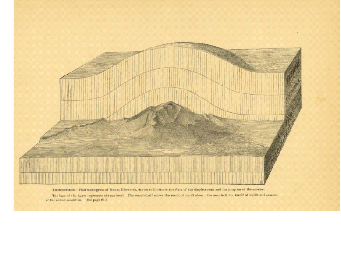
\includegraphics[width=\textwidth]{LEMFinalRevisedmanuscriptDAVFinalrevisions-img/LEMFinalRevisedmanuscriptDAVFinalrevisions-img001.png} 
\caption{The diagrammatic LEM of \citet{Gilbert1877}.}
\label{gilbert_fig}
\end{subfigure}%

\vspace{4em}
\begin{subfigure}[b]{0.7\textwidth}
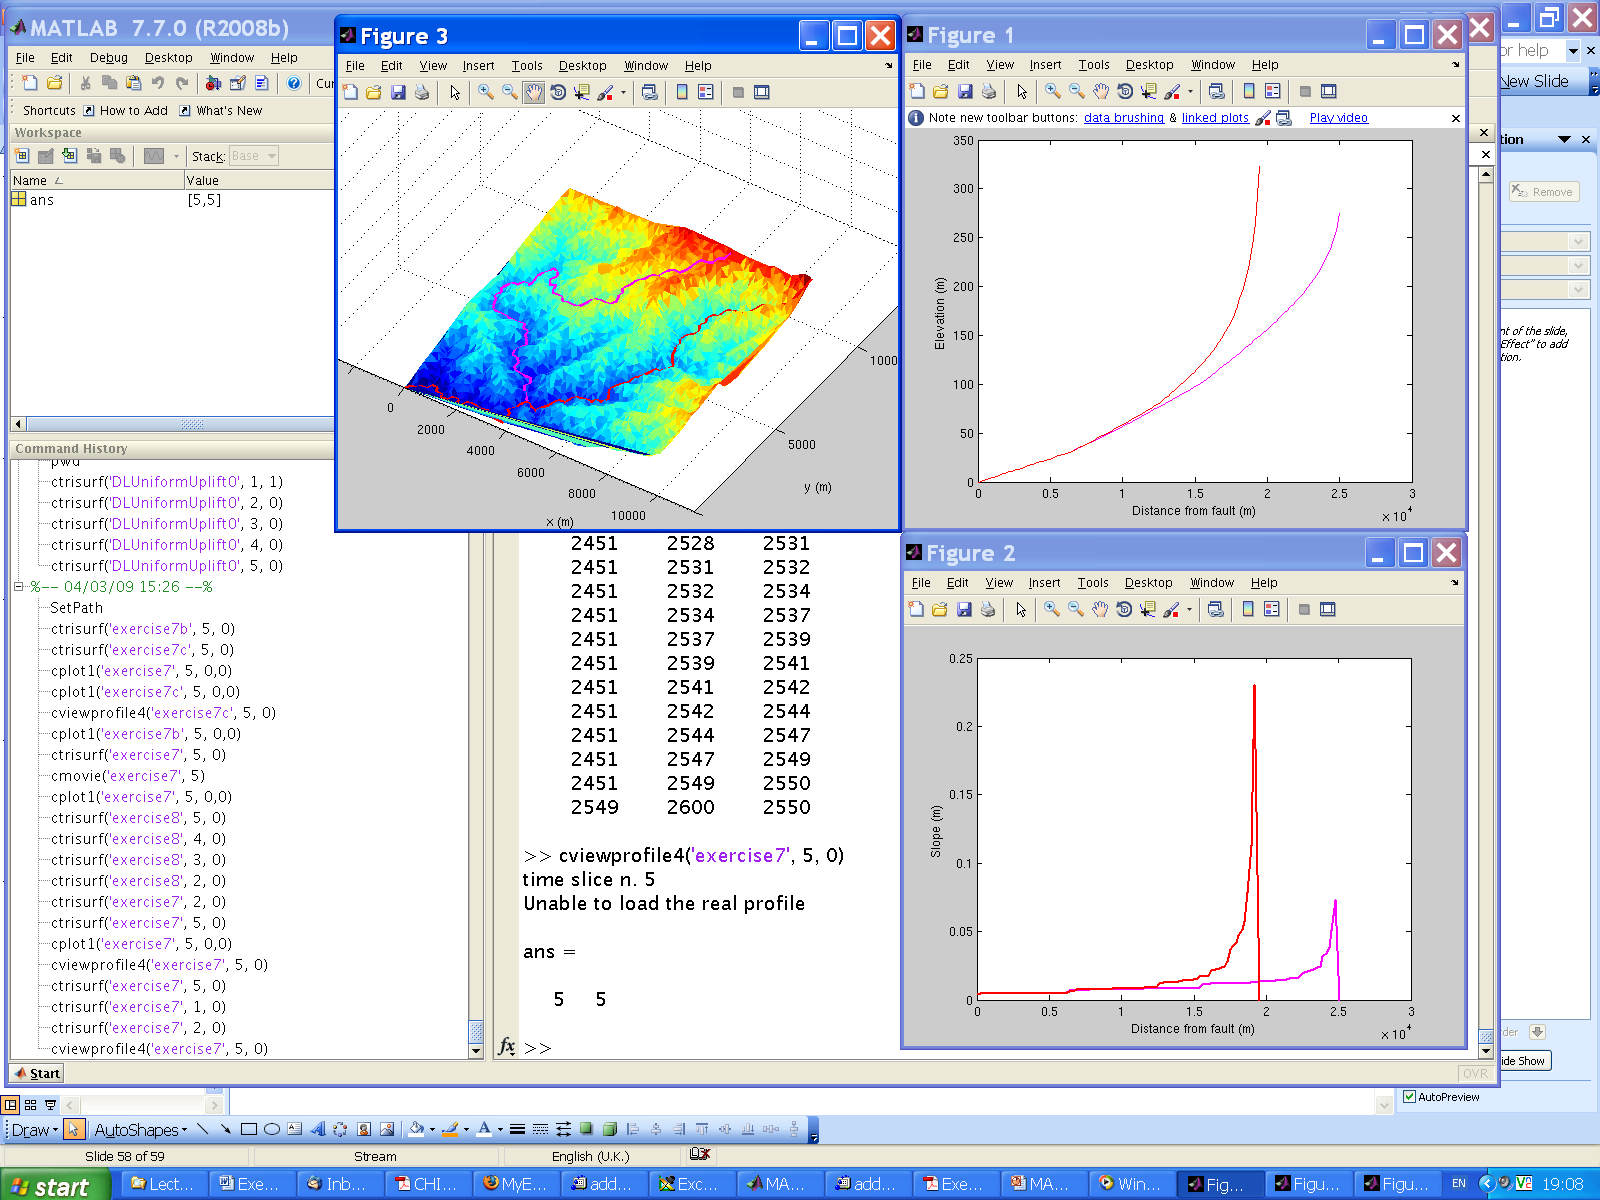
\includegraphics[width=\textwidth]{LEMFinalRevisedmanuscriptDAVFinalrevisions-img/LEMFinalRevisedmanuscriptDAVFinalrevisions-img002.png} 
\caption{A computer numerical landscape evolution model \citep[CHILD,][]{Tucker2001}.}
\label{child_fig}
\end{subfigure}

\caption{The evolution of landscape evolution models.} 
\label{fig_gilbert_child}
\end{figure}



\subsection[Scope]{Scope}
This chapter provides a practical guide to the usage of numerical LEMs. Readers interested in detailed theoretical aspects of landscape evolution modelling should refer to other detailed literature reviews, such as those by \citet{Pazzaglia2003,martin2004numerical,Willgoose2005,Tucker2010}. Other reviews focus on the use and application of LEMs, such as \citet{willgoose2011,van2011modelling,temme2013quantitative}. This chapter is not solely a software-type review of different LEMs \citep[e.g.][]{Coulthard2001}, though comparisons between the features of various LEMs will be made to aid the prospective landscape evolution modeller. In short, the chapter aims to provide an overview of the usage, theoretical background, and software features of mainstream LEMs at the present time.

Physical analogue models of landscape evolution are outwith the scope of this chapter, although numerical LEMs have not replaced their analogue counterparts – nor are they intended to. Physical models are actively used in landscape evolution studies \citep{hancock2002testing,Bonnet2006,Bonnet2009,Sweeney2015}, but such experiments are usually custom-designed to meet the particular needs of a specific research question, and the materials available to construct the analogue model. In numerical landscape evolution modelling, there is more of a collective move (perhaps subconsciously) towards using a small number of community-developed numerical models, which are freely available to the modelling community.

The LEMs discussed in this chapter are primarily designed to simulate processes in humid--temperate sub-aerial environments. The role of glacial or aeolian processes are undoubtedly important in landscape evolution, but are frequently overlooked by the current range of available models, though a range of glacial-specific models exist \citep[e.g.][]{Braun1999,Tomkin2007,Herman2008,Egholm2011,Egholm2012}. Coastal, glacial, and aeolian processes are currently better catered for in environment-specific models. However, the range of geomorphic process representation in more generic LEMs continues to expand and develop.

\section{Fundamentals of Landscape Evolution Models}

\subsection{Governing Equations}

LEMs are ultimately driven by a set of mathematical equations: the \textit{geomorphic transport functions}, often termed `laws' \citep{dietrich2003geomorphic,Tucker2010}. These laws may be derived from physical first principles, empirical evidence, or sometimes a combination of both. When implemented in a model, these laws are applied to a series of discretised cells or nodes representing the landscape. Conservation of mass is applied when calculating the fluxes in and out of neighbouring cells or nodes. The most common assumption made in most LEMs with respect to conservation of mass is that each column of rock or regolith has discrete boundaries between layers of different densities (Figure \ref{fig_conservation_mass}), i.e. there is no allowance for a dynamic variation of density throughout each column in the model. Some models may further assume a uniform layer of substrate with no separate regolith layer. With these assumptions in mind, the majority of LEMs use a mass balance equation of the form:

\begin{equation*}
\frac{{\partial}\eta }{{\partial}t}=B-{\nabla}q_s
\end{equation*}

\noindent
where $\eta $ is the surface elevation, \(t\) is time, \(B\) is a source such as the rate of sediment production, uplift or subsidence rate, and  ${\nabla}q_s$ is the divergence of flux of material – what comes in minus what goes out -- in the x and y directions (after \citet{Tucker2010}, eq. (3).)

\begin{figure}[t]
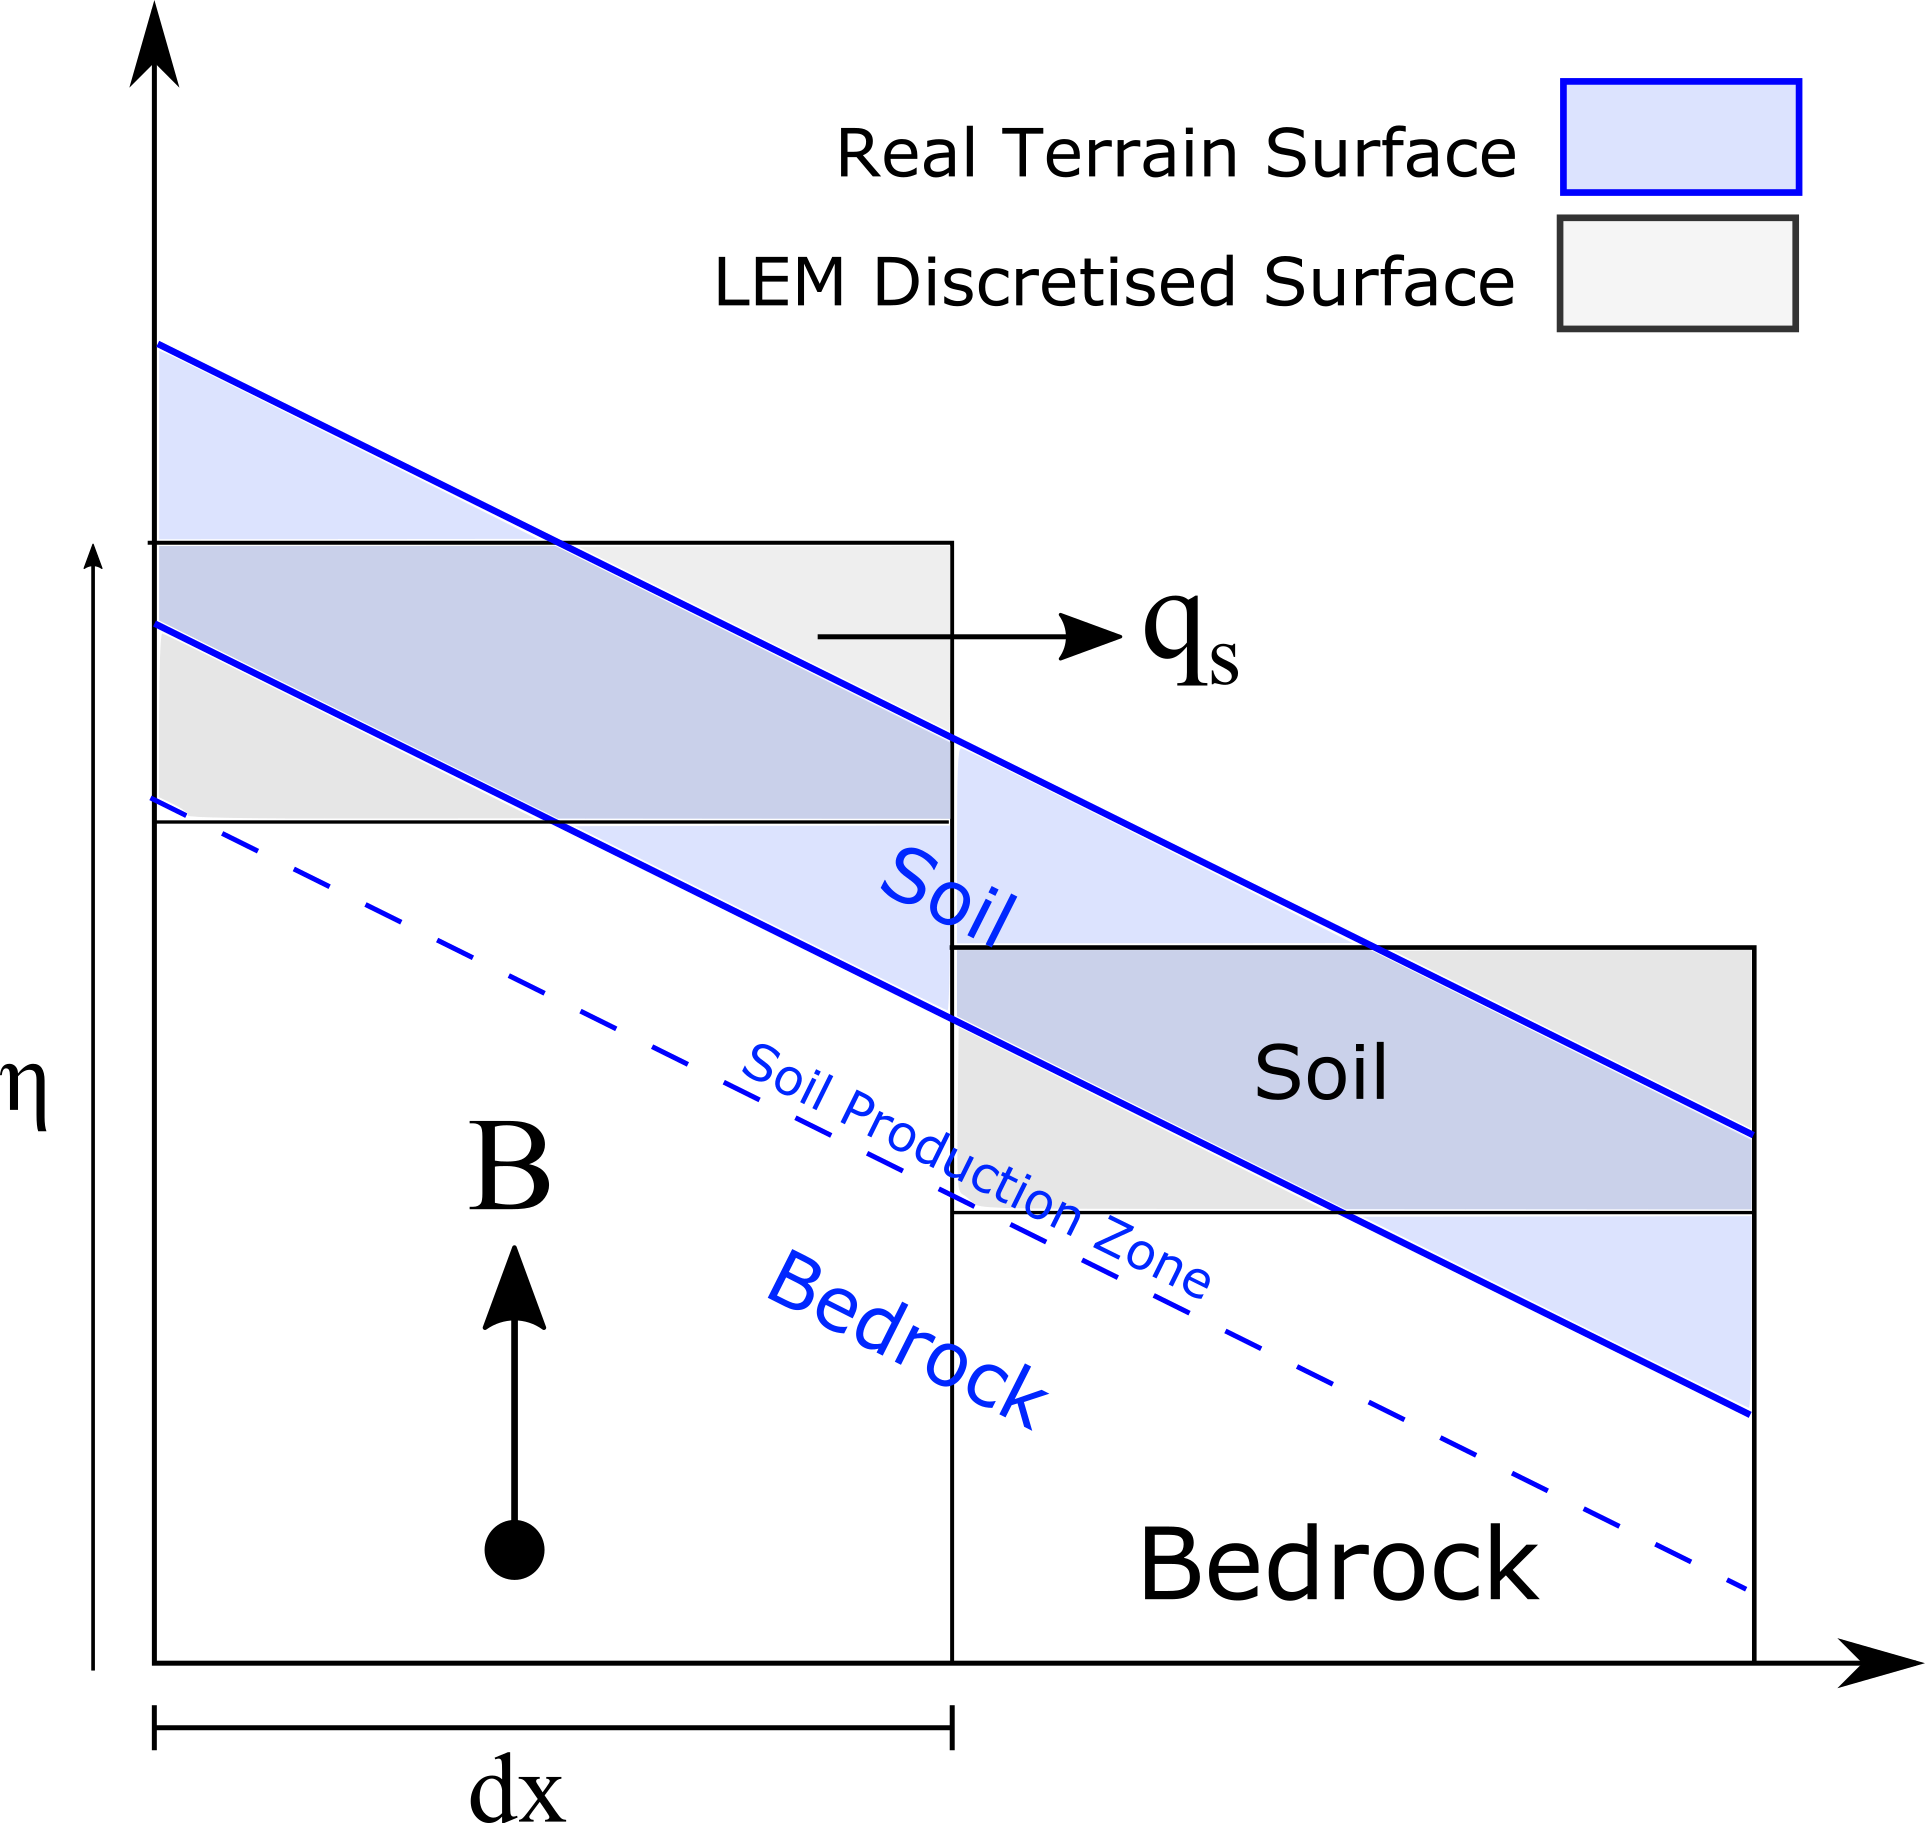
\includegraphics[width=11cm]{LEMFinalRevisedmanuscriptDAVFinalrevisions-img/LEMFinalRevisedmanuscriptDAVFinalrevisions-img003.png} 
\caption{Conservation of mass in a soil mantled landscape or sediment covered channel (after \citet{dietrich2003geomorphic,Tucker2010}). $\eta $ is the surface elevation, \(B\) is the boundary (base-level) change, \(q_s\) the sediment transport term, and \(dx\) the grid cell size in a discretised landscape (assuming regular grid-spacing in this example).}
\label{fig_conservation_mass}
\end{figure}

The modeller must be aware of which equations are implemented in the chosen LEM. Simpler models may be based on a single equation for each process represented, or even a single geomorphic transport function representing bulk processes, such as the hillslope diffusion equation \citep{Culling1960}. More complex models offer the user a wide range of governing equations to select from – this allows comparisons to be made from using different theoretical models of sediment erosion and transport. The Channel-Hillslope Integrated Landscape Development (CHILD) model \citep{tucker2001child}, for example, allows the user to select from several different governing equations for sediment transport, fluvial incision, and hillslope erosion.  

Each of these laws is based on a set of assumptions about the environments that they represent. The selection of the appropriate geomorphic transport law may be scale dependent. The basic stream power law, for example, does not scale well when applied to drainage basins below around 1 km\(^2\) in area \citep{Hergarten2015,Stock2003}.

\subsection{Realism and Prediction}

An important question to ask in the selection of an LEM is what degree of physical realism is sufficient and appropriate for the hypothesis being tested. Models with a strong physical basis, for example those based on computational fluid dynamics (CFD) such as OpenFOAM \citep{Jasak2007}, or SPHysics \citep{Gomez-Gesteira2012}, may be appropriate for studying landscape evolution on very small scales, at the level where forces from multi-directional fluid flow and particle motion form part of the hypothesis \citep[e.g.][]{Bates1998,Jackson2015}. The trade-off in using such models is the increased computational expense, which is why they are infrequently used in studies of landscape evolution beyond small scales.

The question is often posed whether LEMs can be used as truly predictive tools to make quantitative, accurate, and confirmable predictions about how landscapes will respond to future environmental changes at human timescales \citep{hooke2003predictive,pelletier2015forecasting}. Recently, however, some authors have used LEMs to make quantitative forecasts about the evolution of landscapes in very specific environments, such as the response of coastal cliff erosion to climate change over the next century \citep{Hackney2013}, and the evolution and remediation of former quarries and tailings from mining operations \citep{Hancock2004,Hancock2015}.

\section{Technical Implementation}
\label{sec_technical}
LEMs are designed to simulate the evolution of topography over a discretised x, y, z landscape surface, as shown in Figure \ref{fig_main_LEM_components}. Often, this type of model is referred to as a 3D or `whole-landscape' model \citep{Willgoose2005}. The term `2.5D' is sometimes used as most LEMs do not explicitly use a vertical coordinate representing the position of terrain in the vertical. Instead, the vertical dimension is modelled implicitly as a variable for each (x, y) grid cell. LEMs are implemented over a fixed spatial extent (the model domain), with pre-defined boundaries, as denoted by the x and y directions in Figure \ref{fig_main_LEM_components}. 

\begin{figure}[t]
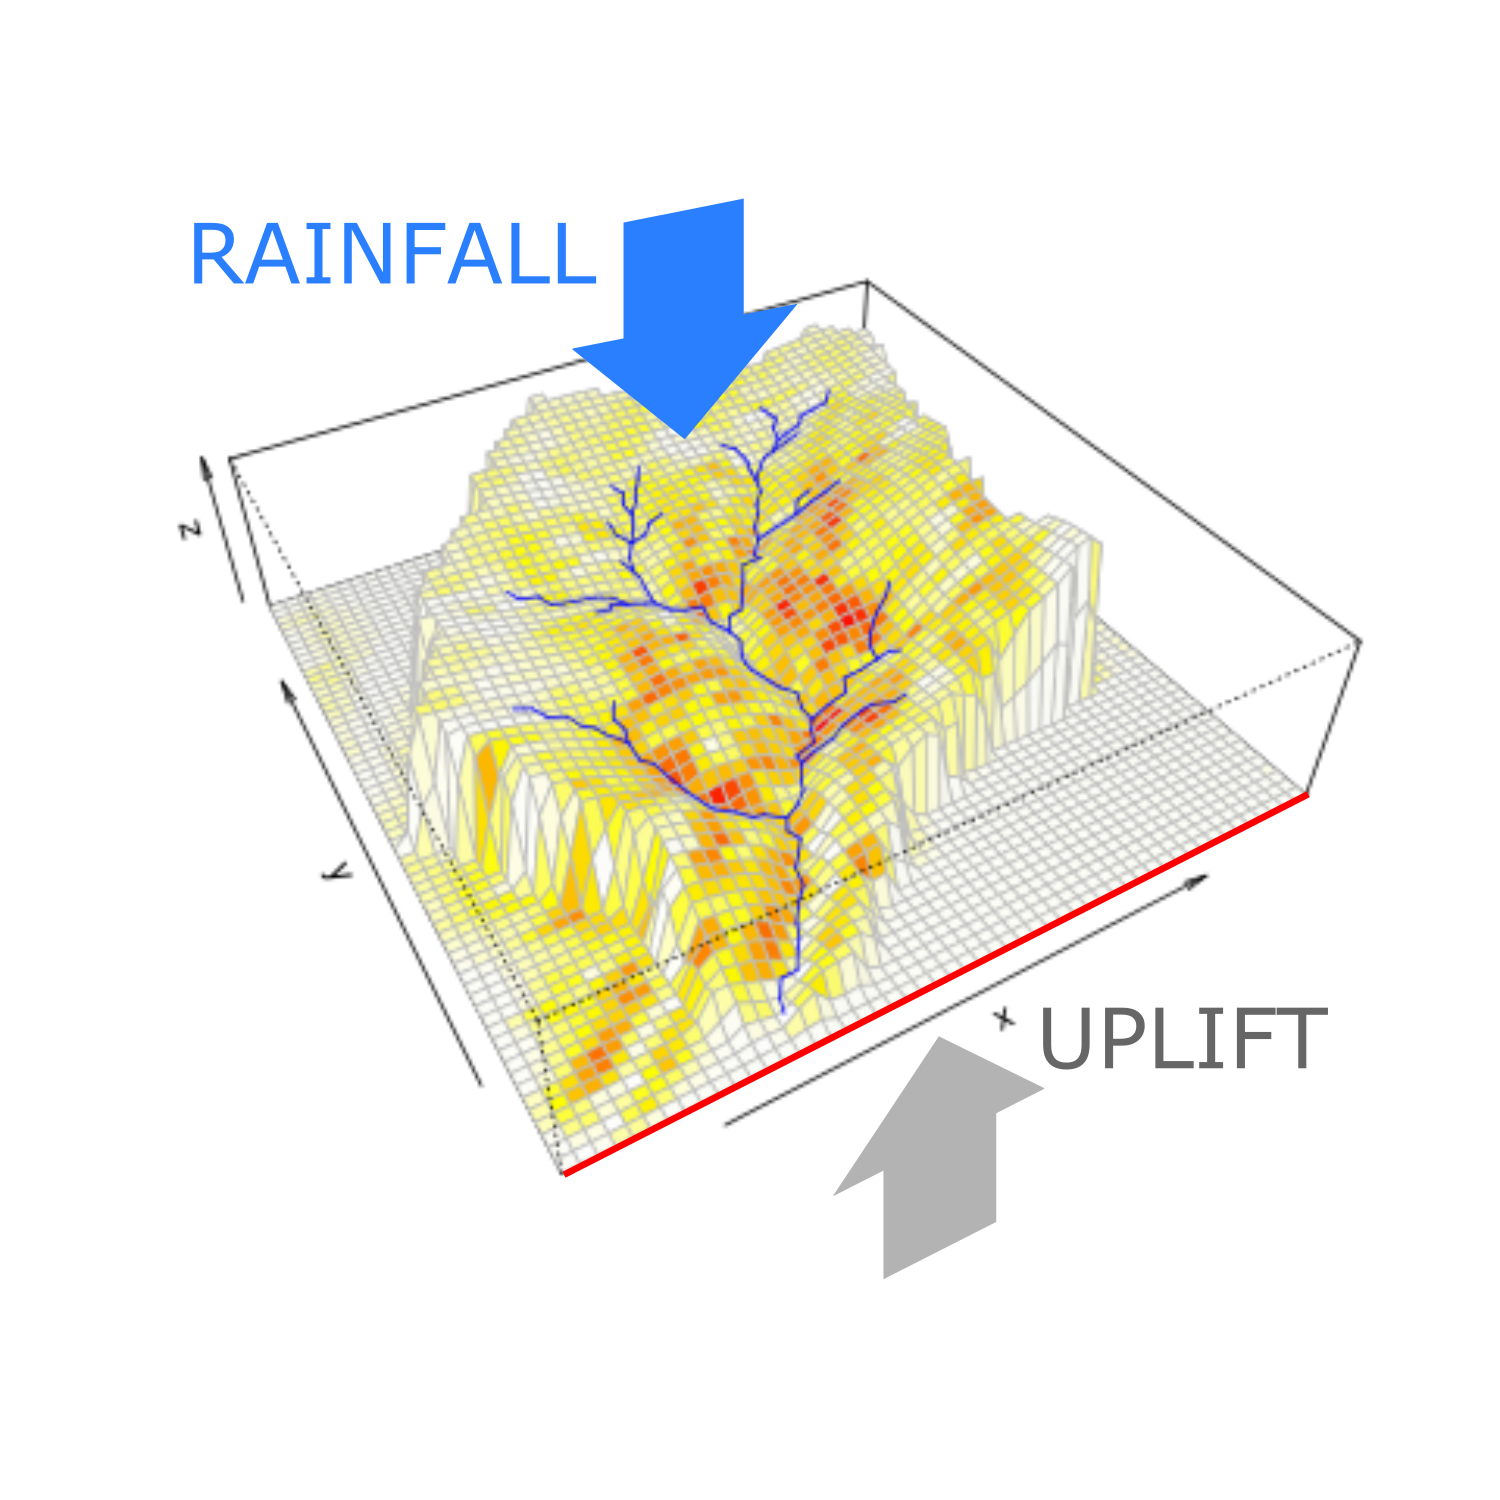
\includegraphics[width=11cm]{LEMFinalRevisedmanuscriptDAVFinalrevisions-img/LEMFinalRevisedmanuscriptDAVFinalrevisions-img004.png} 
\caption{Main components and boundary conditions of a landscape evolution model. Boundary conditions include the climatic, tectonic and base-level conditions (rainfall and uplift), as well as the conditions specified on the model domain edges, such as where water and sediment can leave the model domain (shown by the red line). Channel network shown by blue lines. Erosion rate (red-yellow) is shown as a grid cell variable in this example.}
\label{fig_main_LEM_components}
\end{figure}


\subsection{Grid and Discretisation}
The grid or mesh representing the land surface may be regular (rectilinear cells) or irregular, such as a triangular irregular network (TIN). The discretisation method of the terrain, and for rectilinear gridded domains the grid-cell size, dictates the length scale of landscape features that can be resolved in the model. Figure \ref{fig_LEM_discretisation} depicts a typical regular gridded model domain. In this case, the maximum resolution of the river channel (in blue) is limited to the grid cell size of the model domain, or digital elevation model (DEM) used to initialise the model. Consideration should be given to whether the input data and model domain are of fine enough grid-spacing to resolve geomorphic features of interest.

\begin{figure}[t]
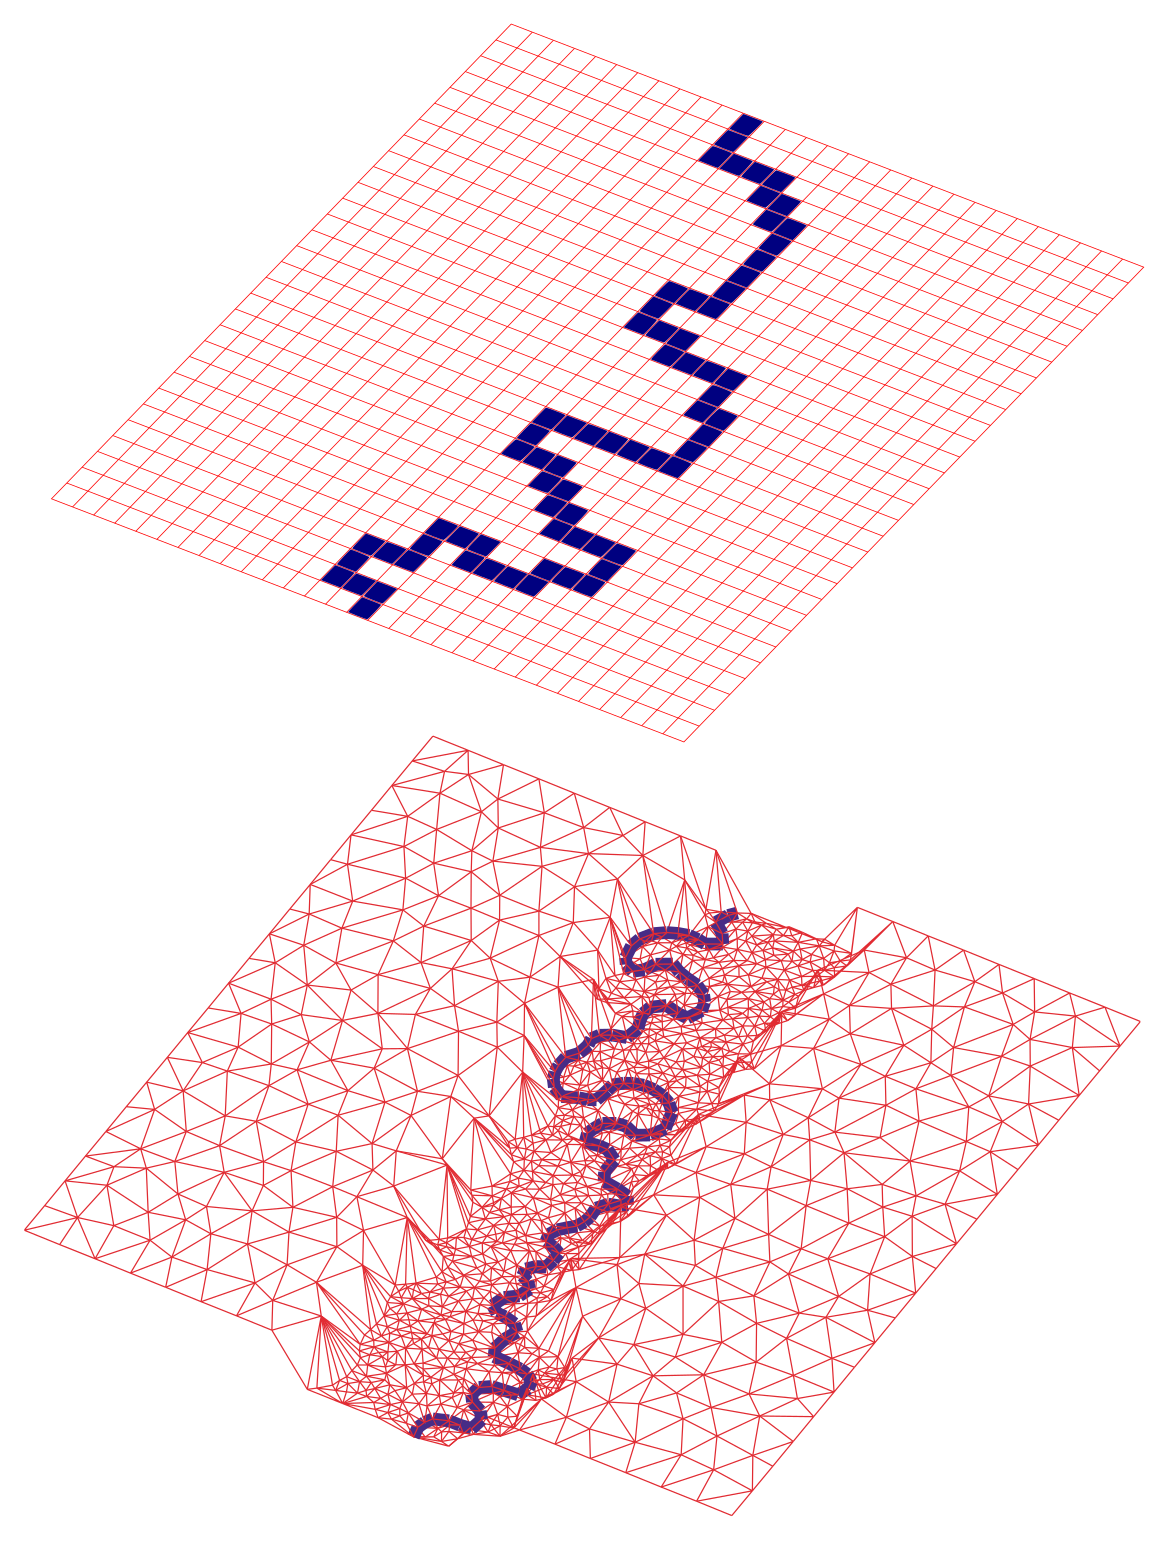
\includegraphics[width=11cm]{LEMFinalRevisedmanuscriptDAVFinalrevisions-img/LEMFinalRevisedmanuscriptDAVFinalrevisions-img005.png} 
\caption{A comparison of two terrain-discretisation approaches. (Top) Regular, rectangular gridded discretisation. (Bottom) TIN, (Triangulated Irregular Network), with adaptive re-meshing. (Re-drawn from Tucker, et al. 2001b).}
\label{fig_LEM_discretisation}
\end{figure}

The advantage of irregular gridded models is that they allow adaptive re-meshing to finer grid-spacing (Figure \ref{fig_LEM_discretisation}) where detailed resolution of certain geomorphic features is advantageous, such as in river channels or gullies \citep{Braun1997,tucker2001child}. Triangular irregular networks also have advantages for the representation of drainage networks – flow routing is not restricted to 45 degree increments as it is in regular, square-gridded models \citep[Figure \ref{fig_LEM_flow_routing}][]{tucker2001child}
In regular gridded LEMs, the grid cell size is uniform across the entire model domain. Regular gridded models dominate the current range of models, being computationally less expensive, and having a source code structure that is often easier to understand, if modifications need to be made. Regular gridded models are more easily compatible with the common raster formats of DEMs, such as TIFF and ASCII raster data, as well as other data inputs derived from remote sensing such as land-use, soil moisture, and vegetation cover.

\subsection{Surface Flow Routing}
In real landscapes surface water may flow in multiple directions over terrain, but in LEMs flow direction is limited by a flow-routing algorithm and the discretisation scheme representing the land surface. The simplest square-gridded models route water from a single cell into one of either 4 or 8 adjacent cells, based on the path of steepest descent (Figure \ref{fig_LEM_flow_routing}), known as the D4 or D8 algorithms \citep{ocallaghan1984extraction}. D8 algorithms, though simple, tend to be too convergent – resulting in a channel network with each stream the width of a single grid-cell \citep{Wilson2008}. More complex algorithms use a scheme where water can be routed in multiple flow directions (MFD) and the total water flux can be apportioned over multiple cells (Figure \ref{fig_LEM_flow_routing}).  However, this class of algorithm tends to be overly dispersive in water flow routing \citep{Wilson2008}. 

\begin{figure}[t]
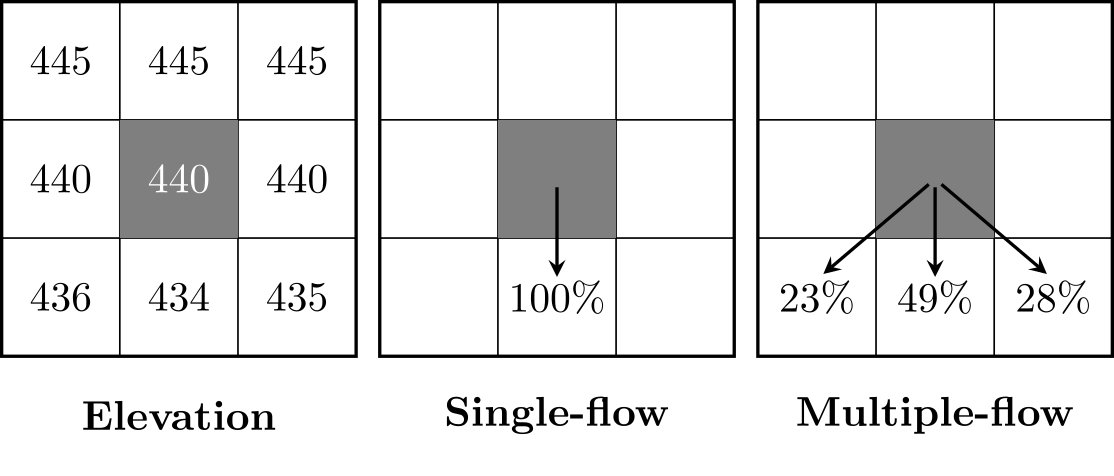
\includegraphics[width=11cm]{LEMFinalRevisedmanuscriptDAVFinalrevisions-img/LEMFinalRevisedmanuscriptDAVFinalrevisions-img006.png} 
\caption{Comparison of single- and multiple flow direction routing methods. (Re-drawn from \citet{Schauble2008}.}
\label{fig_LEM_flow_routing}
\end{figure}

The D-infinity scheme \citep{Tarboton1997} is a single flow direction method aimed at addressing some of the limitations of the standard D8 algorithm. The appropriate scheme depends on the level of realism required for the hypothesis being tested. Simulations of complex riverine processes, incorporating braided channel networks, for example, would require a model with a multiple-direction flow-routing model.\- Flow routing models, with the notable exception of the FastScape algorithm \citep{Braun2013}, are typically the most computationally expensive part of a landscape evolution model, involving many iterative calculations per grid cell or node.

\subsection{Data Input Sources}

For modelling of real landscapes, thought must be given to the source data used to initialise the landscape surface in the model. In simulations of large-scale landscape evolution (model domains of tens to hundreds of kilometres), input data resolution can be relatively coarse, such as a 90 m SRTM-derived (Shuttle Radar Topography Mission) DEM. Even this resolution may be higher than necessary and DEMs may be coarsened through resampling with GIS software in order to reduce the total number of grid cells and hence computational expense. Higher resolution DEMs are necessary for modelling small-scale features, such as gully formation or hillslope erosion \citep{Nearing2010}. It may be necessary to acquire sufficiently high resolution data, on the order of metres to centimetres, from sources such as airborne LiDAR \citep{gallay2013direct}, terrestrial laser scanning \citep{lemmens2011terrestrial}, or structure from motion techniques \citep{micheletti2015structure}. In short, the appropriate resolution of input data is dictated by the length scales at which the geomorphic processes of interest operate.

\subsection{Boundary Conditions}
Thought must also be given to the boundary conditions of the model domain. Boundary conditions refer to any input or constraint on the x, y, z minima and maxima of the model domain (Figure \ref{fig_main_LEM_components}), including tectonic or base-level change, and climatic input, such as precipitation. Most models will operate on the principle of having at least one open boundary where water or sediment can flow out. In some models the placement of boundary outlets is customisable by the user (e.g. CHILD, FastScape). The LEM user should also consider the possibility that these boundary conditions may not be fixed over time, such as variation in rainfall rate or uplift rate. In some situations, the boundary conditions may exhibit feedback with the internal processes of the model domain \citep{Raymo1992,Willett1999}.

\section{Current Models}
LEM development has bloomed in the previous two decades, in part due to significant and continued computational advancement, and there is now a wide variety of models to choose from. The range of models available vary in their complexity, applicability to different timescales, and different process representation. In this section, some of the existing LEMs currently in common use are briefly reviewed.

\subsection{CAESAR-Lisflood}
A family of related models have developed from the original CAESAR LEM \citep{coulthard1996cellular,coulthard2002cellular}. The original CAESAR model is a cellular automaton model that simulates water flow across the landscape, fluvial erosion, sediment deposition, and hillslope processes. CAESAR-Lisflood \citep{Coulthard2013}, the current iteration of the model, uses a more physical-based surface water flow component based on a simplified numerical solution to the shallow water equations \citep[LISFLOOD-FP][]{bates2010simple}. The non-steady hydrological component of the model allows effects such as tidal flows, lake filling, and the blocking of valley floors by alluvial fans to be represented in LEMs \citep{Coulthard2013}. 

CAESAR-Lisflood is suited to simulation of entire drainage basins (in `catchment mode') or sub-sections of a river channel (in `reach mode'), e.g.  \citet{Coulthard2006,van2007embedding}. CAESAR-Lisflood is an appropriate tool for timescales ranging from modelling the effects of a single storm over a few hours, through seasonal, to annual, and millennial time scales of landscape evolution. Process representation in CAESAR-Lisflood is focussed primarily on hydrodynamics and sediment transport, including the simulation of multiple-sized grain fractions. 

Though there is theoretically no upper limit to the time periods that can be simulated with CAESAR-Lisflood, existing studies have focused on shorter scales from decades up to thousands of years, such as simulating sediment output of a small basin under short term climate predictions \citep{Coulthard2012a}, simulating storm and tidal surge dynamics on coastal environments \citep{Skinner2015}, and forecasting the short term geomorphic evolution of former mine-workings and excavations \citep{pasculli2015cellular}.

\begin{figure}[t]
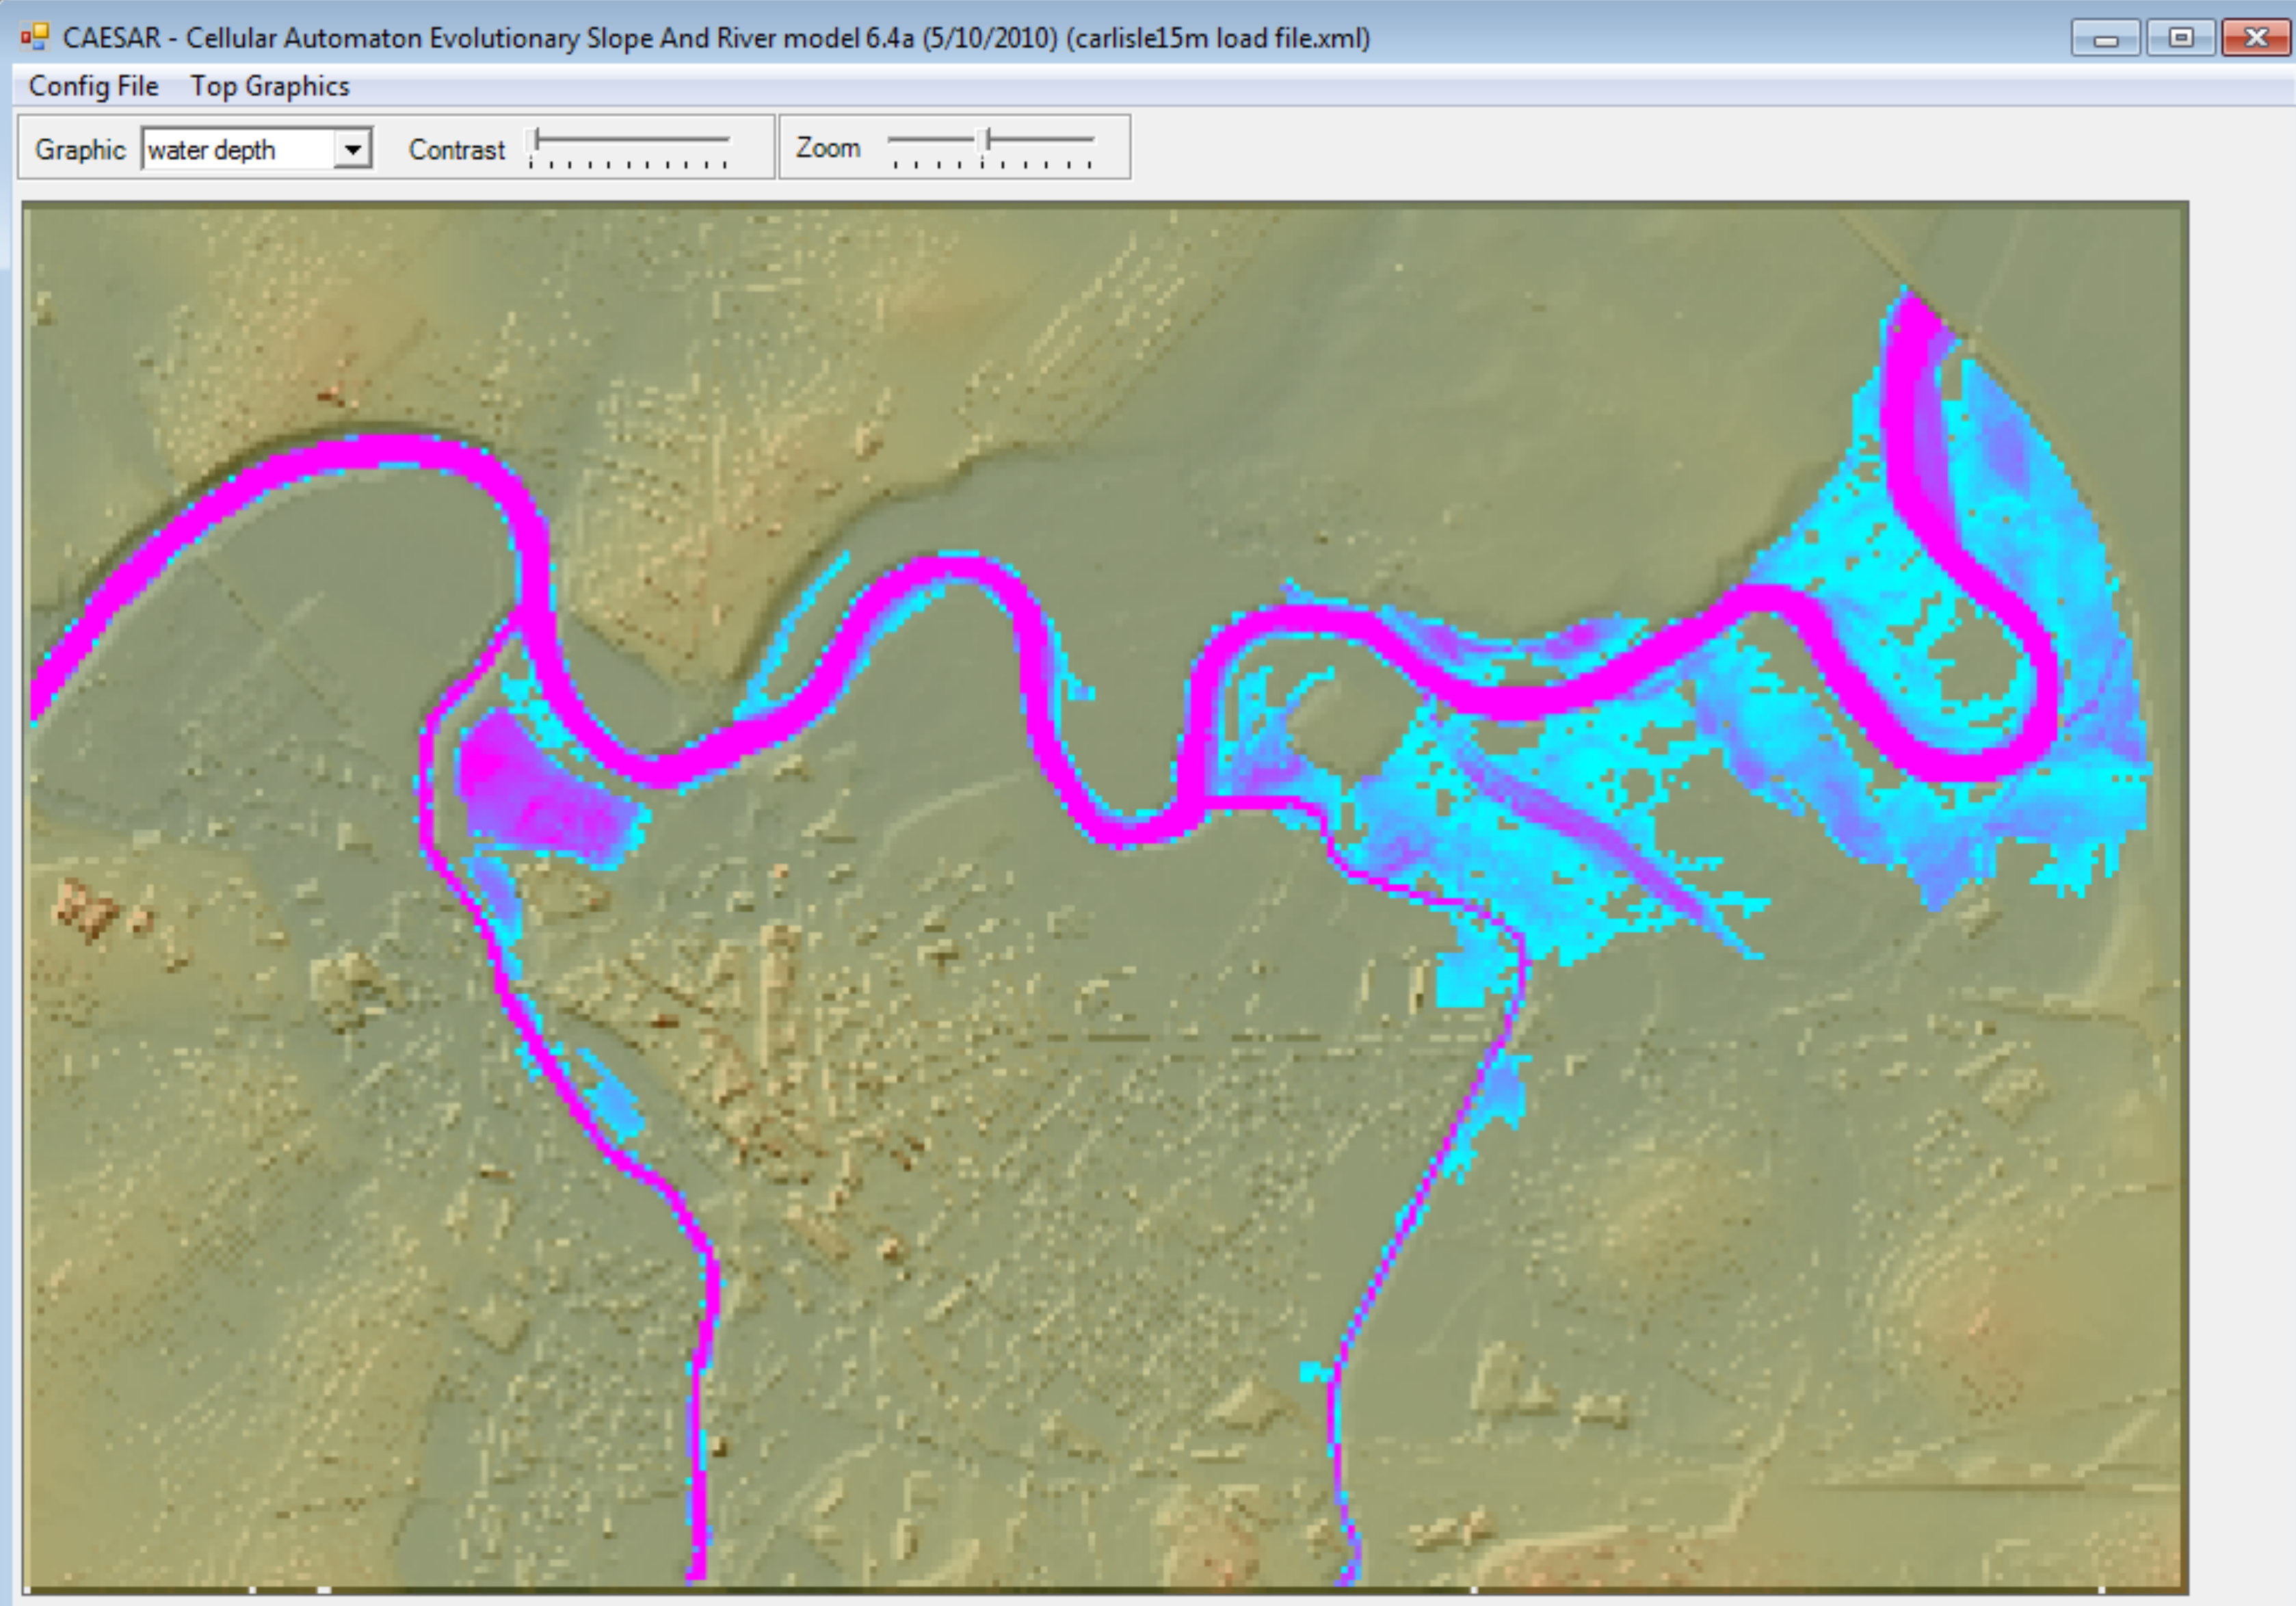
\includegraphics[width=11cm]{LEMFinalRevisedmanuscriptDAVFinalrevisions-img/LEMFinalRevisedmanuscriptDAVFinalrevisions-img007.png} 
\caption{CAESAR-Lisflood simulating the flooding of Carlisle, UK, 2005. Hydrogeomorphic effects of single floods can be simulated in this LEM due to the implementation of a non-steady flow hydrological component \citep{bates2010simple}. Blue to pink colouring represents water depth, with pink indicating the deepest water depths. Model domain 5 km across.}
\label{fig_LEM_CAEASR_Lisflood}
\end{figure}

CAESAR-Lisflood uses a graphical user interface (GUI) to set model parameters and display output (Figure \ref{fig_LEM_CAEASR_Lisflood}). The GUI makes model set-up quick and easier for users with less familiarity with command-line operations or code modification. The current version is limited to running in a Windows-only environment. The integration of visualisation with the core model code also allows the user to view model output as the simulation progresses (Figure \ref{fig_LEM_CAEASR_Lisflood}); this has the advantage of letting the user monitor output without having to wait for a full simulation to complete and visualise the output in a separate step. 

\subsection{CHILD}

The Channel Hillslope Integrated Landscape Development model \citep[CHILD,][]{tucker2001child} is another widely-used model for investigating landscape evolution in a variety of environments, on temporal scales from decades to millions of years. The modular design of the LEM has facilitated its expansion over recent years and it now supports various types of geomorphic process representation. CHILD supports initialisation of the terrain surface from DEM data or generating synthetic topographies from scratch. A wide range of fluvial incision processes can be simulated with CHILD, including both detachment- and transport-limited erosion models, sediment transport, and a range of hydrological and rainfall-runoff generation routines. Recent development of modules has extended process representation to include, for example, modules of dynamic vegetation growth \citep{Collins2004}, floodplain evolution \citep{Clevis2006}, dynamic adjustment of channel width \citep{Attal2008}, representation of sediment grain size \citep{Gasparini2004}, debris flows \citep{Lancaster2003}, and stochastic rainfall generation \citep{Tucker2000}.

CHILD differs from many of the other models described in this section, as it eschews a traditional grid-based spatial discretisation in favour of a triangular mesh, or TIN. As previously discussed in Section \ref{sec_technical}, this allows the model resolution to vary spatially across the domain, becoming higher in regions where smaller scale features and processes operate, such as river meanders, and coarser where features are much larger in spatial extent, such as floodplains and hillslopes \citep{Tucker2001}. 

The CHILD model’s TIN-based approach is advantageous in its flexibility at representing different scale features within a landscape \citep{Braun1997,tucker2001child}, but adds an extra layer of complexity when working with typical raster data formats, requiring conversion between raster and TIN data at the input and output stages of the modelling workflow. A series of MATLAB scripts are provided with the CHILD model for visualising output. The open-source RCHILD package is also available for output visualisation with the R programming language \citep{dietze2014rchild}. The CHILD model is platform-independent (it will run on multiple computer operating systems).

\subsection{FastScape-based LEMs}

FastScape is an algorithm based on an efficient implicit numerical scheme to solve variants of the stream power law for modelling large scale landscape evolution \citep{Braun2013}. The major advance made by the FastScape algorithm was to increase the efficiency of the flow routing calculation – a bottleneck in most LEMs -- and hence the model is useful for rapidly testing hypotheses of landscape evolution. Several related LEMs have been based on an implementation of the FastScape algorithm, including:

\begin{itemize}
\item The `original' FastScape LEM \citep{Braun2013}
\item DAC -- the Divide and Capture model \citep{Castelltort2012,Goren2014}
\item LSDTopoTools: Raster Model (\url{http://lsdtopotools.github.io})
\end{itemize}
Recent applications of FastScape-based LEMs have focused on the simulation of synthetic landscapes under differing tectonic, lithological, and climatic boundary conditions \citep{Braun2013,Braun2014,Castelltort2012,Yang2015}. The FastScape LEM also allows for the use of DEM data to set the initial surface topography in the model. An optional GUI interface is also included with the FastScape LEM, though this is currently only functional in Linux-based environments. The underlying FastScape algorithm is generic, and not necessarily tied to any particular LEM – users may choose to implement the algorithm in other open source models.

\subsection{LAPSUS}
The LAPSUS model (Landscape Modelling at Multi-dimensions and Scales) is a modular, multi-process model suited to studying catchment-scale erosional processes and landscape evolution at a range of temporal scales from years to hundreds of thousands of years  \citep{schoorl2000three,van2015lapsus}. LAPSUS is suited to studying landscape evolution by means of soil and sediment redistribution through processes of fluvial erosion, surface wash, landsliding, tillage, creep, and tectonics. Applications include studying the interaction of non-linear processes in landscape evolution \citep{Temme2009,Schoorl2014}, the role of tillage and changing land-use in decadal to millennial scale landscape evolution \citep{Schoorl2001,Baartman2012b}, the sensitivity of soil erosion to rainfall intensity \citep{Baartman2012a}, and exploring uncertainty and parameter choice in landscape evolution modelling \citep{Temme2011}. LAPSUS features a graphical user interface similar in appearance to the CAESAR interface in Figure \ref{fig_LEM_CAEASR_Lisflood}, allowing a similar visual monitoring of model outputs to take place without further post-processing required.  

\subsection{Other LEMs}

Landscape evolution modellers have a vast choice of models at their disposal: the organisation CSDMS (Community Surface Dynamics Modelling System: \url{http://csdms.colorado.edu}) operates as a de facto model repository for developers and users of LEMs. The terrestrial model section lists well over one hundred different models that have been published to the site. CSDMS is a useful starting place for potential modellers to select an LEM based on their own requirements.  

%A summary of some of the more commonly used models over the last decade is presented in Appendix B, showing the key features of each model for comparison. 

Some LEMs extend the functionality (and often complexity) of existing models. For example, the CAESAR-Lisflood-DESC model \citep{Barkwith2015} features, in addition to the core components of CAESAR-Lisflood, modules for distributed surface and soil hydrology, groundwater hydrology and a more physically realistic representation of landsliding. Applications of CLiDE have included the prediction of geomorphic and environmental hazards over human timescales \citep[e.g.][]{tye2013nene,Barkwith2015}. 

The current range of LEMs includes well established software packages such as the SIBERIA and CASCADE models. SIBERIA \citep{Willgoose1991a} is a square gridded model originally developed to investigate the feedbacks between hydrology, catchment form, and tectonics \citep{willgoose1994hydrogeomorphology}. CASCADE \citep{Braun1997} was an early implementation of a TIN-based model designed to simulate long-term landscape evolution as a function of fluvial and hillslope processes.  Though the deployment of these two models has declined in recent years somewhat, they continue to be used as a benchmark for inter-model comparison in some studies \citep[e.g.][]{Hancock2015}.

Recent developments within the modelling community have extended traditional modelling functionality with other elements of geomorphic analysis.  The LSDTopoTools software (\url{http://lsdtopotools.github.io}), for example, features an LEM based on the FastScape algorithm, integrated within a set of powerful topographic analysis tools. This allows easy transition between modelling and analysis of the results using common and novel topographic metrics. 

Another recent development is the Landlab software package \citep{hobley2017creative}, which takes a highly modular approach to numerical modelling of landscapes. The user can rapidly create their own bespoke LEM from a set of existing components. This results in a high degree of user control over the complexity of the model configuration, not only in terms of process representation, but also the effect that technical aspects, such as grid type and flow routing algorithm have on model performance and output. The modular design avoids the usual expenditure of re-writing commonly used codes for process representation, model gridding, and standardised file input and output. A key strength of Landlab is its accessibility to users who do not have significant prior experience in designing and implementing numerical codes, but wish to embark on model development. Examples of Landlab's applications include the study of impact cratering on landscape evolution \citep{hobley2013modeling}, the impacts of wildfires on hydrologic response \citep{adams2017landlab}, quantifying the link between regolith production and subsurface temperatures \citep{barnhart2014chilly}, investigating the response of landscape evolution under non-steady state hydrology \citep{adams2017landlab}, and as a basis for developing a stochastic cellular automaton model \citep{Tucker2015}.

The selection of LEMs discussed here range from those that have already established a wide user-base in landscape evolution research (e.g. CHILD, CAESAR, LAPSUS), to newer developments that offer novel functionality or process representation for modellers (e.g. Landlab, CLiDE, DAC, LSDTopoTools). This chapter is not an exhaustive list of landscape evolution models, and some previously popular models have been omitted as it was felt they have been superseded or subsumed by newer offerings. The range of LEMs discussed here should nevertheless provide a starting point for tackling a wide range of modelling endeavours. A table summarising the main features and processes represented in each LEM is given in Table \ref{fig_LEM_comparison}.

\begin{sidewaystable}[t]
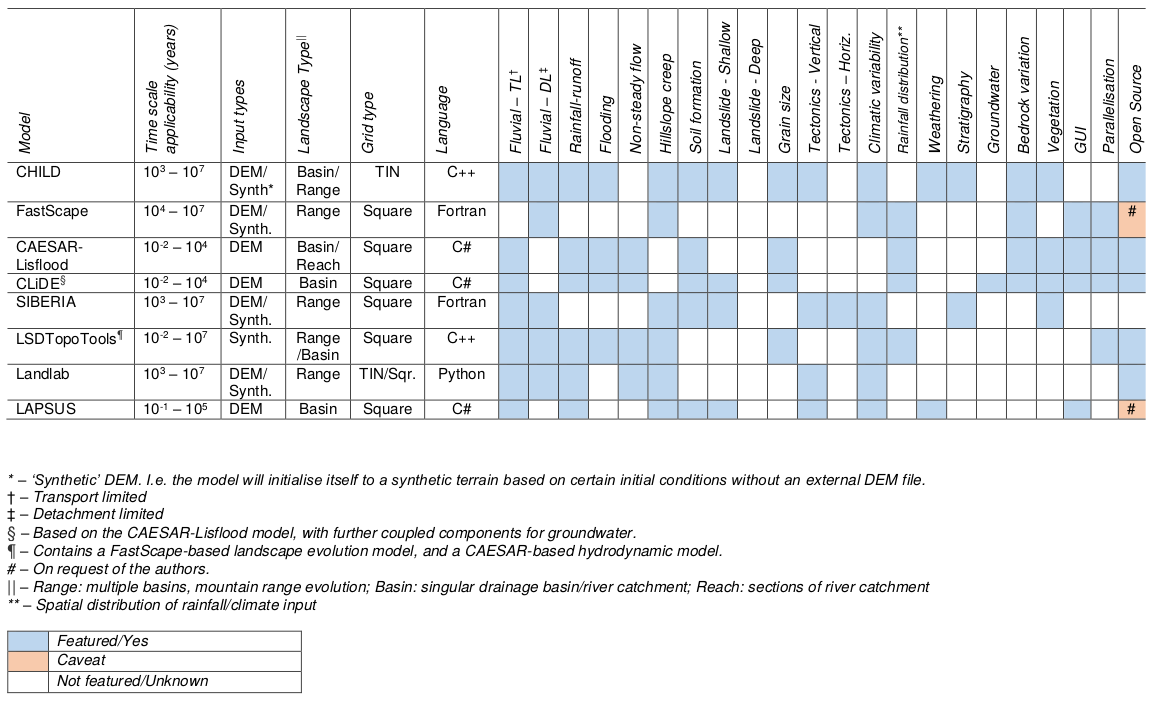
\includegraphics[width=24cm]{LEMFinalRevisedmanuscriptDAVFinalrevisions-img/table_lems_comparison.png} 
\caption{Feature comparison of widely used landscape evolution models. Process representation shown by model in blue/pink/white matrix.}
\label{fig_LEM_comparison}
\end{sidewaystable}

\section{Uncertainty, Sensitivity, and Calibration}

\subsection{Uncertainty}
Uncertainty in modelling describes our inability to know precisely the initial conditions of a model, to represent in a model all the processes that govern landscape evolution, and ultimately to know with certainty the accuracy of the predicted outcome \citep{Beven1996,pelletier2015forecasting}. All LEMs make simplifications regarding process representation, partly due to a lack of detailed knowledge in how certain processes work, and partly due to limitations about how these processes can be represented in computer models.  Uncertainty may also stem from inaccuracies in input data sources, the choice of model parameters, and the boundary conditions of the model (and whether these parameters and boundary conditions might change through time). Uncertainty in LEMs may lead to errors that propagate through the simulation and increase in magnitude as a simulation progresses. 

Ideally, one should address uncertainty by first assessing which parameters the model is most sensitive to -- it may be that large uncertainties in one parameter have relatively little effect on the model outcome, whereas small uncertainties in a different parameter produce unexpectedly large variation in the model outcome \citep{pelletier2015forecasting}.

Methods such as ensemble analysis should be considered, whereby multiple instances of the same simulation are run, with a range of parameters chosen from a probability distribution to assess the most likely outcomes from a model. While uncertainty cannot be removed entirely from modelling studies, it is useful to be able to state the most probable outcome(s), based on a probabilistic distribution of input conditions.

Uncertainty is a particular challenge in landscape evolution modelling as many processes are threshold dependent \citep{snyder2003importance}, or scale non-linearly \citep{schumm1979geomorphic}. In choosing parameter values, guidance can be taken from published values of such parameters derived for similar environments, particularly when they have been calibrated with field data, where available \citep[e.g][]{Temme2011,Hancock2015,Mudd2014}.

\subsection{Sensitivity and Calibration}
Following earlier definitions \citep{oreskes1994verification,Trucano2006}, calibration is defined here as the selection and modification of input parameters of a model in order that they maximise agreement with observed data in real landscapes. Such parameters in LEMs might include the coefficient terms in fluvial erosion laws, for example the \(K\), \(m\), and \(n\) parameters in the stream power law \citep{seidl1992problem}, hydrological parameters such as Manning's \(n\) \citep{manning1890flow}, or the threshold shear stresses required to initiate erosion \citep{snyder2003importance}. Many such parameters are not directly quantifiable by field measurement, and model users should consult similar studies for recommended values, or conduct their own sensitivity analyses to constrain uncertainty in parameter choice. Other parameters may lend themselves to more rigorous methods of calibration, where they link directly or indirectly to measurable values in the field. Examples would include the calibration of hydrological parameters to produce a `best fit' with observed discharge values at river gauging stations \citep{Coulthard2013,wong2015sensitivity} and constraining stream power law parameters using statistical models and sensitivity analyses \citep{Croissant2014,Mudd2014}.

\section{Validation \& Confirmation}
Validation is the process of assessing the legitimacy of a model set-up. Results from a model may or may not be valid depending on the quality of input data and model parameter choice \citep{oreskes1994verification}. Moreover, validation does not necessarily establish the truth or accuracy of model predictions, only that the model is internally consistent. In practice, it can be thought of as a `sanity check' on the input to the LEM before beginning the simulation. For example, is the input DEM of sufficient resolution to represent the scale of geomorphic features expected to be formed? Do the input parameters conform to observed or realistic ranges? If the answer to these types of question is `no', the model predictions will be invalid. 

Geomorphologists use LEMs to deduce whether hypotheses about landscape evolution are likely to be valid, which requires a method for assessing how the model output supports the hypothesis. Confirmation refers to the assessment of how model predictions -- after selecting suitable input parameters -- match observations in nature \citep{oreskes1994verification}. Directly observing landscape evolution is challenging at human timescales, as whole-landscape change occurs at slow pace, making direct confirmation of model predictions difficult in many situations \citep{Hasbargen2003,hoey2003testing}. Some predictions made by LEMs, however, can be directly or indirectly confirmed to a certain extent with field observations. This includes short term phenomena such as gully formation, coastal erosion, and river bank incision. At short timescales, direct monitoring and quantification of erosion rates, particularly in rapidly eroding fluvial settings, becomes feasible. 

\subsection{Field Confirmation}
Techniques to indirectly measure the rates of landscape change are wide-ranging, and include measuring sediment flux at catchment outlets, using traps to measure bedload erosion and deposition \citep{Bunte2004}, bedload impact sensors \citep{rickenmann2007continuous,turowski2010partitioning}, suspended sediment measurements at gauging stations \citep{brazier2004quantifying}, and the use of radio frequency identification-tagged sediment particles to track sediment movement \citep{chapuis2015coupling,Beer2015}.

Through the rise of digital photogrammetric techniques, such as airborne and terrestrial laser scanning, direct measurement of whole-landscape morphological change is now possible at high enough resolutions to quantify small differences in topographic features, particularly in rapidly evolving landscapes \citep{rosser2005terrestrial,vaaja2011mapping}. Using these methods to aid model confirmation would be limited to small scale studies, as processing of point cloud data from these sources can be highly computationally expensive \citep{axelsson1999processing}. 

At longer, geomorphologically significant timescales, a range of techniques becomes available to assist in the calibration of LEMs and confirmation of hypotheses. Optically stimulated luminescence dating uses a property of quartz and feldspar minerals that records the amount of time they have sat in a sedimentary or soil deposit, which can be used for dating landforms \citep{aitken1998introduction,Stokes1999a,Murray2000}. The applicability of this technique to different temporal scales is site-specific and ranges from years to upwards of hundreds of thousands of years. Cosmogenic radionuclide (CRN) dating is a technique based on the interaction of cosmic rays with certain isotopes in minerals in the Earth's surface \citep{Anderson1996,dunai2010cosmogenic}. The production rate of certain isotopes can then be used to determine absolute ages and erosion rates in the landscape. A recent application combining an LEM with a model of CRN production rates is found in \citet{mudd2017detection}, where it is used to explore the detection of transience in landscapes. The method is suitable for determining ages up to about 4 million years \citep{Burbank2011}.

\subsection{Topographic Metrics}
In the past, looser forms of qualitative assessment have been used where LEMs are applied in an exploratory manner, such as to test mathematical models of geomorphic processes, or make speculative predictions of landscape evolution. In this sense, topographies generated by LEMs can be compared to real landscapes that they are intended to represent. Visual inspection of real versus simulated terrains can provide some degree of hypothesis confirmation \citep{bras2003six,hooke2003predictive}. However, it is recommended that this approach be extended to quantitative analysis by using a range of topographic metrics to compare simulated topographies with their natural counterparts. Such metrics include: mean relief, slope, river profile concavity, channel steepness indices \citep[e.g.][]{wobus2006tectonics}, terrain curvature, hypsometry, and roughness. A similar technique of comparing LEM output to physical analogue models has also been implemented by \citet{hancock2002testing}. 

A range of techniques is available to assist the modeller in assessing model predictions and confirming hypotheses of landscape evolution. The most appropriate methods will depend on the time-scale of the study, and the type of predictions made by the hypothesis. 

\section{Limitations}

Landscape evolution models are based on a body of existing theoretical models describing geomorphic processes. Arguably, one of the greatest limitations in landscape evolution modelling is the lack of unified theories describing key processes in the landscape, such as fluvial incision or hillslope form \citep{dietrich2003geomorphic}. This forces the user to select from an often wide (and still expanding) range of geomorphic transport laws, without sufficient knowledge of the particular landscape equation in question to select the most appropriate law. Sensitivity analyses may help to quantify the uncertainty stemming from this issue.

Long term landscape evolution modelling (on the order of thousands to millions of years) suffers from the issue of how to upscale micro-scale geomorphic processes to the macro-scale. The extent to which quasi-random fluctuations in geomorphic processes, such as turbulent flow in rivers and small-scale heterogeneity in soil or bedrock composition, should be incorporated into long-term laws of landscape evolution laws is not yet fully developed \citep{Tucker2010}. Many LEMs have relied on statistical approaches to deal with this issue \citep{Hovius1997,Lague2005,Lague2013}. However, the scaling exponents and statistical distributions in these parameterisations are often based on limited empirical evidence from field observation.

Numerical landscape evolution modelling is also bound by limitations of computing power available to the user. Considerations have to be made when designing LEM experiments in order that the simulations can be carried out in reasonable compute time. Higher grid resolutions and less parameterisation of key processes may lead to more physically realistic simulations, but at increased computational expense. Recent releases of some LEMs have begun to tackle this by incorporating parallelisation techniques into the model code, taking advantage of multi-core processors that have now proliferated into most personal computers as well as supercomputers.

\section{Conclusions}
When considering the use of landscape evolution models in geomorphological research, the modeller must make key decisions at certain stages of the modelling process. The modelling process can be summarised as follows: 

\begin{enumerate}
\item Definition of the research aim and purpose of the model.
\item Selection of appropriate model and components. 
\item Choice of input data if applicable. 
\item Selection and calibration of model parameters, possibly including sensitivity analysis to address uncertainty. 
\item Validation of model set-up – is the choice of parameters and input data logical and internally consistent?
\item Confirmation of model predictions against observed data. 
\item Interpretation of model predictions. 
\end{enumerate}

There are two factors that should be considered at each of these stages: scale and process representation. The intended scale of the experiment, both temporal and spatial, has implications for LEM selection (e.g. is the model suitable for the time-scale of interest?). Process representation should also strongly guide decisions at each stage. The user needs to know which laws are implemented in their chosen LEM, and what parameters are associated with them that need to be selected and calibrated. If the model offers a choice of geomorphic process laws to choose from, which is the most appropriate for the environment that the experiment is intended to emulate? 

Landscape evolution models are powerful tools for the geomorphologist. Like all powerful tools, however, care must be used to avoid unintended consequences from misuse. Numerical LEMs have heralded a new era in geomorphic research, and are increasingly used to address important research questions in geomorphology. They aid both our understanding of how geomorphic processes work, and our ability to make quantitative predictions about landscape change in the future.


% Chapter 3 is an overview of meteorlogical data sources and model data.
\chapter{Integration of rainfall radar data with a landscape evolution model}
\label{chapter_metdata}
\chaptermark{Linking rainfall radar data with LEMs}

%%%%%%%%%%%%%%%%
% TO DO
% 
% Figures of total rainfall accumulation over catcments
% Zoomed in location maps
%
%%%%%%%%%%%%%%%%
%\begin{chapquote}{Claude Monet \textit{}}
%``It's enough to drive one crazy, trying to depict the weather, the atmosphere, the ambience...
%\end{chapquote}

\section{Introduction}
%This chapter discusses the various sources of meteorological data and numerical models used to generate rainfall input to the landscape evolution models discussed in Chapters \ref{chapter_landscape_evol} and \ref{RainfallInLEMs}. In this thesis, two sources of rainfall data were used to drive the hydrological inputs of landscape evolution models: precipitation radar data from the UK 1km rainfall radar composite product (Section \ref{NIMROD}) and rainfall outputs from a numerical weather prediction model (Section \ref{WRF}

Measuring and predicting rainfall has been a central activity to meteorological and hydrological sciences for centuries. The importance of having good estimates of rainfall for understanding hydrological processes was recognised by \citet{perrault1674}, particularly for understanding the role of rainfall in the water cycle \citep{biswas1970history}. Historically, the earliest hydrometeorological observations in Britain were recorded by Bede the Venerable (AD 672--735) \citep{mcculloch1993history}. Quantitative measurement of rainfall with instrumentation in the UK is attributed to Christopher Wren and Robert Hooke \citep{biswas1970history}, who developed a precursor to the modern tipping-bucket raingauge, although numerous records of rainfall measurement have been noted in other societies predating efforts in Britain \citep{strangeways2010history}. Quantifying the amount of rainfall that has fallen in a given area over a period of time is referred to formally as \textit{quantitative precipitation estimation} \citep{fabry2015radar} and its prediction ahead of time as \textit{quantitative precipitation forecasting} \citep{golding2000quantitative,browning2003quantitative}.

In the context of landscape evolution and erosion modelling, realistic rainfall input sources are often a secondary consideration, with many models using a uniform rainfall rate across the model domain, or generating rainfall inputs artificially from stochastic rainfall generators \citep[Chapter \ref{chapter_RainfallInLEMs},][]{Tucker2000}. Despite the paucity of realistic rainfall data use in landscape evolution modelling, there is no shortage of rainfall data at the disposal of the landscape evolution modeller. This chapter explores some of the potential meteorological data sources that could be incorporated into numerical models of landscape erosion and evolution, and presents a software framework for processing rainfall radar data for use in the CAESAR-Lisflood landscape evolution model, and its derivative models.

\subsection{Rainfall data sources}
% Raingague
Direct measurement of rainfall is accomplished through the use of rainfall gauges, which provide in situ measurement of rainfall totals, and in some cases, instantaneous rainfall rates, at a fixed-point location. In the UK, the density and spacing of rainfall gauges is heterogeneous at the individual catchment scale, though there is good coverage at regional to national scale. At catchment and sub-catchment scale, however, most rainfall gauge networks are too sparse to provide detailed information about the distribution of rainfall variability within a catchment. Exceptional coverage is sometimes found in catchments that have been instrumented as `research catchments', where a high-density network of gauges has been established for monitoring of specific catchments, \citep[e.g. the Plynlimon research catchment,][]{newson1979results} but this is atypical. Though raingauges are reliable for point totals of rainfall, common types of gauge (such as the widespread tipping-bucket raingauge) have a tendency to underestimate true rainfall rates during very high rainfall intensities \citep{habib2001sampling,ciach2003local}. Nonetheless, the rain gague data is used extensively for verifying and calibrating other indirect measurements of rainfall, such as satellite or radar \citep{harrison2000improving,ebert2007methods}, or predictions from numerical weather forecast models \citep{golding2000quantitative}.

%Satellite
Indirect measurements of precipitation can be either \textit{active} or \textit{passive} in their mode of measurement. Active sensors emit a pulse of electromagnetic radiation, usually in the microwave--radiowave band depending on the application, and measure the amount of energy reflected back from hydrometeors \citep{fabry2015radar}. A mathematical function is used to convert the measurement of reflected electromagnetic radiation into a rainfall rate or rainfall amount, the choice of function depending on the particular method used. Passive sensors, as their name implies, do not actively emit any kind of electromagnetic radiation directly, but measure only the radiation emitted naturally from the Earth's surface. When precipitation is present over the surface, passive sensors measure the brightness temperature\footnote{Brightness Temperature is a descriptive measure of radiation in terms of the temperature of a hypothetical blackbody emitting an identical amount of radiation at the same wavelength.} from the surface, and use this measurement to determine the phase and intensity of rainfall present based on a number of physical and empirical conversion formulae. Many satellite precipitation measurement missions combine active and passive sensing to build a complete picture of rainfall on the Earth's surface (e.g. the \textit{Tropical Rainfall Measurement Mission}, TRMM, \citet{simpson1988proposed}, the \textit{Global Precipitation Measurement Mission}, \citet{hou2014global}). The advantage of satellite precipitation measurements lies in their ability to cover large regions of the globe, which would be infeasible with a network of ground-based measurements. Satellite precipitation measurements are particularly useful at increasing the coverage of rainfall measurement over the oceans, where there is a particular paucity of other measurement sources. Limitations in satellite precipitation measurement include its lower resolution compared to ground based measurements, due to the distance between the surface and the orbiting sensor, as well as the lack of coverage around polar regions on most satellites. Due to the orbiting nature of satellites, they cannot currently take measurements with the same frequency as ground-based methods. Typical temporal resolution of satellite measurements is on the order of 1.5--3 hours, whereas ground-based methods can take measurements up to every few minutes. Consequently, space-borne measurements are not usually suitable for applications requiring high-frequency, high-resolution measurements of rainfall, but lend themselves well to providing consistent, near-global coverage (with the exception of polar regions). 

%Radar
Ground-based precipitation radars are active sensors, emitting pulses of electromagnetic radiation in a 360\degree \ field of view through a rotating antenna. They measure the intensity of the beam that is reflected and use this to derive a rainfall rate through a series of empirical formulae \citep{wilson1979radar}. The scanning beam is angled slightly above level (typically 5\degree) allowing a near-surface measurement of rainfall at close range, which gradually becomes higher as the beam extends in range.  Rainfall radars have a large variety of ranges depending on application, but national weather service radar stations typically have a range of 200--500 km in diameter \citep{fabry2015radar}.  

\subsection{Advantages of radar for hydrological applications}
Weather radar is particularly well suited to use in hydrological applications, and for the purposes of this thesis, by extension, to landscape erosion models that feature a hydrological component. There are two principal hydrological applications \citep{harrison2012radar}: 1) routine monitoring of precipitation for climatological data collection, day-to-day river management, weather forecasting, and model validation; 2) early detection and prediction of floods for civil protection purposes. Both applications have common requirements such as data accuracy, but early flood detection has the added need for rapid estimation and dissemination of rainfall rates in order to give as much lead time as possible to authorities responsible for flood prediction and mitigation \citep{fabry2015radar}. 

Rainfall radar is particularly useful in small catchments, where response times to intense rainfall events are short, and where rapid rises in river level can quickly overcome infrastructure such as flood defences, reservoirs, and dams. With smaller catchments, the likelihood of having other sources of rainfall and hydrological information diminishes, such as rainfall and river flow gauges \citep{fabry2015radar}. In larger catchments with adequate gauging facilities, precipitation may have large variability in spatial patterns, necessitating the use of other methods to determine the distribution of rainfall inputs into a river catchment. Large, mountainous catchments also benefit from rainfall radar as they may experience intense localised rainfall and quickly channel the rain from steep hillslopes into gorges and river channels.



\subsection{Basic principles of Radar}

Radar works on the principle of emitting microwaves and measuring the intensity and time taken of waves reflected back from distant hydrometeors. The use of radar to detect distant rainfall was alluded to by \citet{marshall1947measurement} who wrote: 

\begin{quotation} 
``\textit{It may be possible therefore to determine with useful accuracy the intensity of rainfall at a point quite distant (say 100km) by the radar echo from that point}".
\end{quotation}

The basic principle of rainfall radar remains the same to this day, though technological advances have increased the quality and speed of dissemination of rainfall measurements. Specifically, meteorological radar measures the reflectivity, and uses this value to determine the intensity of rainfall through an empirical formula relating reflectivity intensity to a rainfall rate. This is refereed to as the Z--R relationship, where \(Z\) is the reflectivity and \(R\) is the rainfall rate. Many variants of the formula exist, taking the general form of:
  
\begin{equation}
Z = aR^b
\end{equation}

\noindent
where \(a\) and \(b\) are empirically-derived constants \citep{gunn1949terminal,joss1969raindrop}.

\subsection{Processing and error correction}

The reflectivity returns measured at any individual radar site are a combination of the radar waves reflected off hydrometeors at the scan level at a given moment in time, plus any other objects or obstacles in the path of the radar, plus a level of background noise from the atmosphere and instrument. From receiving raw radar return signals, there follow several steps to process this data and convert it into a usable rainfall product, giving an accurate estimate of surface rainfall. Post-processing steps can be summarised as follows:

\begin{enumerate}
\item Noise removal. Background noise may come from instrumental sources or sources in the atmosphere. A typical approach to noise removal is to estimate the mean noise from scans take on precipitation-free periods and subtract this from the measured return reflectivity.

\item Removal of non-precipitation echoes. Sources of non-precipitation echoes include insects, birds, air and shipping traffic, and interference from other radar emitters. There are several approaches to removing this type of echo, some combining several techniques into one \citep{germann2006radar,rico2008classification}.

\item Removal of blocking obstacles such as terrain. Radar scans made at low elevations suffer from blocking of the emitted signals by topography. The effects of blocking on radar reflectivity can be modelled using a high resolution digital elevation map and a model of radar beam propagation \citep{pellarin2002hydrologic}. Another approach is to use long term records of reflectivity and rainfall rate to extrapolate rainfall rates in the blocked regions.

\end{enumerate}

\section{Rainfall radar in Britain and Ireland}

Britain and Ireland are covered by a network of C-band (5 cm wavelength) radar stations. Fifteen of these stations are located in the UK and maintained by the UK Met Office, two in Ireland are maintained by Met {\'E}ireann. A further radar is located on the island of Jersey, maintained by Jersey Met. Combined, these sites give coverage of the whole of Britain, Ireland, and surrounding waters (Figure \ref{fig_radar_map}). The scanning pattern of the radar network returns radar reflectivity data at four elevations every five minutes, at a resolution of 600 m by 1\degree, extending to 250 km in range \citep{harrison2012radar}. 



\begin{figure}[htb]
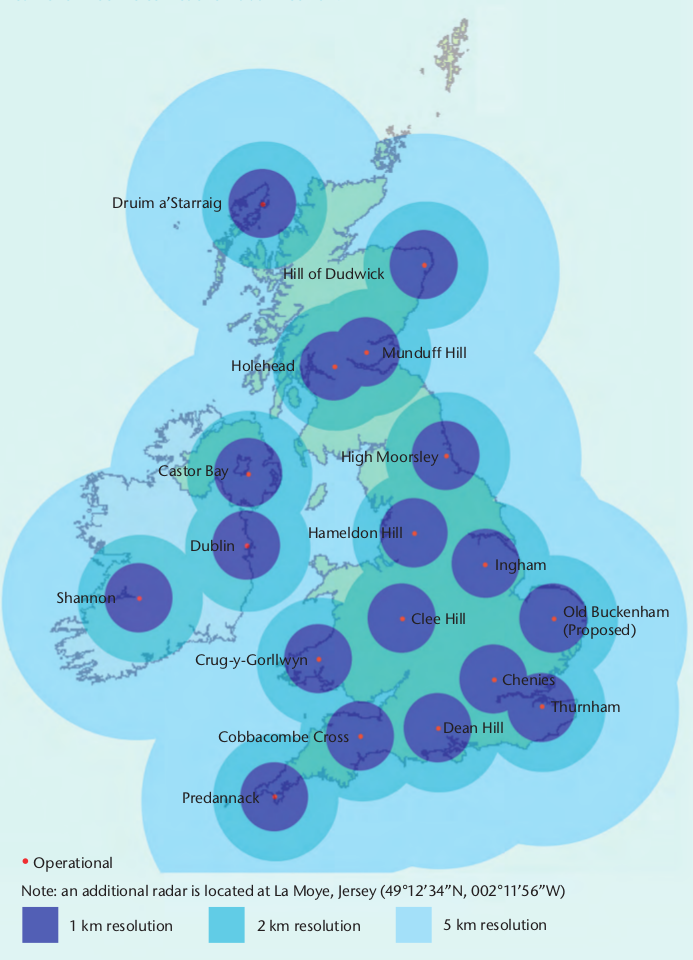
\includegraphics[width=11cm]{chp_radar/radar.png}
\caption{Network of weather radar stations in the British Isles and Ireland. \textit{Source: National Meteorological Library, Met Office, UK.}}
\label{fig_radar_map}
\end{figure}


\section{UK 1km Radar Composite Product}
After processing and error correction of raw radar returns, the rainfall data still exist in a non-gridded format for each individual radar site and the surrounding scan-area. This intermediate format is unsuitable for many applications in environmental modelling and climatology, as adjacent radar sites may report different rainfall rates at locations covered by the overlap of neighbouring radar coverages. To produce a national-scale gridded rainfall data product for the UK, single-site rainfall estimates are composed into a unified data product with a domain covering 47$^{\circ}$--62.7$^{\circ}$N, 13.47$^{\circ}$W--4$^{\circ}$E \citep{metoffice2003nimrod}. Where grid points are covered by overlapping rainfall estimates, the radar with the highest `quality index' -- a function based on the height of the lowest usable radar scan -- is used in the composite data product \citep{harrison2009high}. Other approaches for generating composite radar data products use weighted inputs based on the quality of all radars that provide coverage for a given location \citep{peura2007using}. The finalised UK radar composite product consists of five-minute data at 1 km grid spacing on a regular Cartesian grid. The data is supplied in a proprietary binary format and requires further data processing for ingestion into other models or subsequent analysis. %The code developed to convert this is shown in Appendix 

\section{Use in landscape evolution models}
No currently available landscape evolution models have the capability to directly ingest spatially variable rainfall data from meteorological data sources, such as radar composite products or rainfall data from numerical weather prediction model output. This was a key limitation of current landscape evolution models identified in Chapter \ref{chapter_RainfallInLEMs}. The CAESAR-Lisflood model is capable of ingesting spatially variable rainfall data, but not directly from meteorological data formats, though previous efforts have been made to manually process radar data for the CAESAR-Lisflood model using GIS (Geographic Information System) software \citep[e.g.][]{coulthard2016sensitivity}. The current lack of an automated framework for processing gridded meteorological data for landscape evolution modelling studies substantially slows down research workflows and brings the potential for introducing error or inconsistency between similar studies. Current best-practice advice is to devise automated tools to ensure data processing workflows are reproducible \citep{wilson2014best}.

\subsection{Linking gridded rainfall data with the CAESAR-Lisflood model}
A software framework is presented for processing gridded meteorological rainfall data for ingestion into a landscape evolution model.

Radar data from the UK 1 km composite data product is provided in binary format covering the whole UK \citep{metoffice2003nimrod}. To extract the data for the study area and convert it to a suitable format for the CAESAR-Lisflood model, a further series of post-processing steps are required. The required inputs to the CAESAR-Lisflood model for spatially variable rainfall are:

\begin{itemize}
\item A \textbf{hydroindex grid} file used to mark zones of the catchment that receive different amounts of rainfall throughout the simulation. The hydroindex file has the same dimensions and grid-cell size as the main input terrain DEM in the model.
\item A \textbf{rainfall timeseries} file. This file lists the rain rate at each time step (by row) for each one of the hydroindex zones (by column).
\end{itemize}

The workflow for producing these input files from the radar composite product is:
\begin{enumerate}
\item Convert the composite data from binary format to a human-readable text format.
\item Crop and extract the set of radar images for the time period and geographical extent required. (Figure \ref{fig_radar_extract}.)
\item From the extracted radar images, compile the rainfall rate timeseries. The number of `hydroindex zones' corresponds to the number of radar pixels in the extracted radar data subgrids. (Figure \ref{fig_hydroindex} a.)
\item Produce the hydroindex file at the correct grid-spacing, dimension, and geographical extent. (Figure \ref{fig_hydroindex} d.)
\end{enumerate}

Details of how to access the code for the radar data processing software are given in Appendix \ref{appendix_software}.

\begin{figure}[htb]
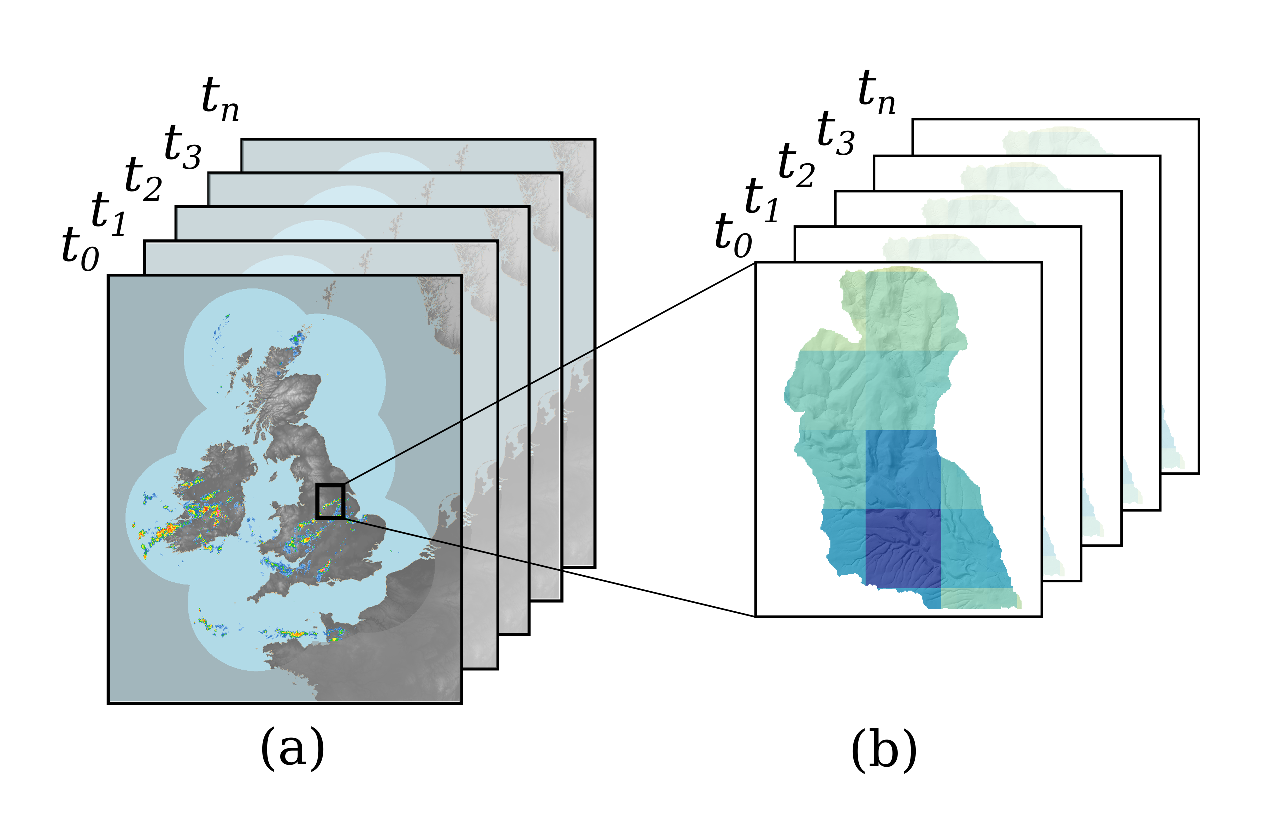
\includegraphics[width=15cm]{chp_radar/cropradar.eps}
\caption{From the UK composite radar product (a), subgrids of the study area extracted for the time period of interest (b). The number of radar image pixels in each subgrid determines the number of hydroindex zones used in the model initialisation.}
\label{fig_radar_extract}
\end{figure}

\begin{figure}[htb]
\includegraphics[width=11cm]{chp_radar/hydroindex.eps}
\caption{(a) Using the extracted radar data subgrids, a timeseries file is created mapping each radar image pixel to a hydroindex zone, for every time step. The hydroindex grid file must be the same dimensions and grid-spacing as the input terrain DEM (b). Numbering each radar image pixel in one of the extracted subgrids (c), the hydroindex file (d), is created from mapping the pixel indexes to the same resolution grid as the terrain input DEM.}
\label{fig_hydroindex}
\end{figure}


\section{Summary}
Rainfall radar is one of many potential sources of rainfall data that can be incorporated with landscape evolution models. Rainfall radar data has several advantages that make it appropriate for use in combination with lansdcape evolution modelling, particularly the CAESAR-Lisflood model. Both model and data source are based on regular, square gridded domains, which makes the translation of rainfall data source to the model input relatively straightforward. The use of other numerical models based on irregular grids, such as the CHILD model,  \citep{Tucker2001}, would require further interpolation steps at the data preparation stage, and possibly at model runtime if the model domain permits adaptive re-meshing \citep{clevis2006simple, tucker2001child}. The CHILD model for example allows the density and location of model grid points to be re-calculated during a simulation to better resolve transient geomorphological features such as river meanders or braided rivers. Fixed gridded models such as CAESAR-Lisflood do not require any grid re-meshing during the model simulation, and the computational costs are potentially reduced for this reason.

For studies using multiple sites and case studies, having a single data source such as a national composite radar product provides a degree of comparability between different sites over different time periods, though upgrades to radar equipment and post-processing algorithms \citep[e.g.][]{harrison2012radar} may negate this advantage if there are large time gaps between case studies, or for long-term studies using rainfall radar data. Rainfall radar's availability in gridded format, and its national coverage availability for the UK since 2004 make it an ideal source of rainfall input data for hydrological and landscape evolution modelling studies. 

The processing framework presented in this chapter provides an automated and reproducible method for extracting sub-regions of gridded rainfall data from the UK 1km composite radar data product and preparing it for ingestion into the CAESAR-Lisflood landscape evolution model and its derivative models.


%
%Rainfall radar are used to infer the spatial distribution and intensity of rainfall over a spatial range of up to several hundred kilometres. Electromagnetic radiation in the microwave spectrum is emitted in pulses through radar antenna that focuses them into a narrow directional beam. When the microwaves encounter hydrometeors (or other obstacles in the path of the beam), the reflected microwave beams are backscattered towards the radar dish. The location and intensity of precipitation can then be calculated using the time taken for the returned radar waves to reach the radar dish, and the amount of backscattered microwave radiation. Radar rainfall measurements are not direct measurements of rainfall, rather they are inferred by making a series of assumptions of how the radar backscatter -- the radar reflectivity -- relates to the quantity and other characteristics of hydrometeors. The amount of radar reflectivity is determined by the size, shape, composition, and distribution of hydrometeors that are sampled by the focused radar beam. Radar reflectivity, denoted by \(Z\), is related to the rainfall rate, \(R\), by the formulation:
%
%\begin{equation}
%Z = aR^b
%\end{equation}

%\section{Numerical Weather Prediction - the Weather Research and Forecasting model}
%\label{WRF}

%Numerical weather prediction models (NWP) are used to predict 


% Chapter 4 is a more focused review of rainfall representation in LEMs
\chapter{Rainfall representation in current landscape evolution models}
\label{chapter_RainfallInLEMs}
\chaptermark{Rainfall representation in current models}

\section{Introduction}
This chapter reviews how current landscape evolution models represent rainfall input into the landscape system. It is worth stating here what exactly is meant by rainfall input, in the context of the atmosphere--land-surface system as represented in numerical models. Perhaps equally as importantly, it is worth discussing what aspects of rainfall are \textit{not} represented at all in any numerical models of landscape evolution, to clarify how geomorphologists conceptually think of meteorological processes acting on the landscape.

For most purposes, rainfall input in landscape evolution models is simply the quantity of water added to a surface cell or node, or to the whole model domain. In practise, no numerical models represent rainfall in the sense of it actually falling from the sky and hitting the ground. While this may seem a somewhat trivial point, the impact of individual rain drops on the land surface is known to be a in important contributor to surface erosion. Rain-splash erosion, as it is termed, is a well-studied phenomenon [cite a review of rainsplash erosion, if there is one?]. The interaction of raindrops with the surface is complex; it depends on the size of raindrop, falling velocity, angle of attack, soil exposure, soil mineralogy, and cohesion of the soil surface. All of these factors could affect both erosion on the landscape hillslopes, as well as the route that water takes to runoff and reach the rivers, before fluvial erosion can happen.

If we briefly turn to physical analogue models of landscapes, rainfall representation implicitly accounts for some of the above factors in rainsplash erosion and runoff, because of the physical need to generate a rainfall source from above the model, such as through a fine-meshed sprinkler [CITE]. In fact, geomorphologists using physical analogue models of landscape evolution attempt a degree of rainfall realism by ensuring the raindrops they generate are reasonably well scaled to the size of their landscape analogue (Meyer, 1994). By contrast, numerical models of landscape evolution begin their representation of rainfall input at the surface -- in effect rainfall input in most landscape evolution models has nothing to do with \textit{falling} rain or its impact on the ground. Conceptually, rainfall input in numerical models is the amount of water that would be added at the surface from one or more (usually many more!) raindrops, once they have reached the ground. It ignores any effects from the physical collision raindrops make with the ground. This simple conceptual model of rainfall input is used throughout the rest of this chapter when referring to rainfall input in landscape evolution models.

\section{Simple models and proxies for rainfall variation}

\subsection{1D models}
Isolated aspects of landscape evolution and hydrology can be studied using 1D models of features such as hillslopes profiles and longitudinal river profiles, or storm hydrographs in the case of hydrology. Though the work in this thesis focuses on 2D models, it is useful to consider the work done by others invesigating the feedback from rainfall variability on 1D models of landscape evolution, before progressing to full 2- or 2.5D\footnote{Occasionally, the terms 2D and 2.5D are used interchangeably when referring to landscape evolution models, although in effect they both produce what looks like a `3D' terrain surface from their ouput. The `third' dimension (or extra 0.5D in 2.5D terminology) comes from the fact that the elevation variable can be used to reconstruct a 3D picture of the landscape based on the value for each grid cell or node. In practice, nearly all of the process models in landscape evolution models are 2D, e.g. water routing over the surface does not account for turbulent flow in x, y and z directions, such as in computational fluid dynamic models. Sediment transport does not account directly for 3D particle motion or collisions between particles. I use the term 2D landscape evolution model throughout the work.} models over an \(x,y\) model domain. 

Roe et al. (2002) modify a simple 1D model for river profile evolution (Seidl and Dietrich 1992; Howard et al., 1994; Whipple and Tucker, 1999) to incorporate a feedback for orographic precipitation based on changing elevation along a steepening river profile. Their precipitation feedback model accounts for two precipitation regimes: the first typical of midlatitude, shallower, and narrower mountain ranges such as the West coast of North America, and one for broader and taller ranges such as the Sierra Nevada, European Alps or the Southern Alps of New Zealand. The former represents rainfall patterns that are dominated by the prevailing upslope winds, increasing precipitation with distance upstream, whereas the latter represents environments where atmospheric moisture content exerts more control over precipitation, resulting in decreasing rainfall at higher elevations, and a rainfall shadow on the leeward side of the range. In a later work (Roe et al., 2003) the 1D model incorporating orographic rainfall feedback is extended to the 1D relief structure of mountain ranges. The maximum relief is found to be strongly dependent on the type of precipitation regime chosen - with the prevailing upslope wind regime favouring lower relief, symmetric mountain ranges, and the atmospheric moisture-limited regime favouring higher relief mountain ranges.

Further 1D models have been developed to determine the relative importance of rainfall variability compared to other boundary conditions, such as tectonic uplift or base level fall. The 1D river profile model of Wobus et al. (2009) uses a transport limited formulation of river profile evolution (Meyer-Peter and Muller, 1948) with a simple parameterisation of rainfall based on modifying the exponent to the discharge-area approximation given by:

\begin{equation}
q_w = k_qA^c
\end{equation}

where \(q_w\) is the water discharge, \(k_q\) a dimensional coefficient, \(A\) the contributing drainage area, and \(c\) the exponent that relates which portions of the drainage basin contribute to gathering precipitation and converting it to water discharge. A decrease in \(c\) represents a shift to more rainfall being gathered in the upper reaches of the stream. An increase in \(c\) represents rainfall being gathered in the lower reaches. The situation where \(c = 1\) implies rainfall input is equal along all sections of the river profile. The end result is perhaps intuitive -- more rainfall input in the upper reaches of the stream (decrease in \(c\) ) results in more incision in the headwaters. However, the study reveals a key difference in the way that climatic and tectonic signals propagate along a river channel. Numerical results show that rainfall-driven perturbations propagate from the channel head downstream, whereas tectonic perturbations invariably propagate from base-level upwards towards the channel head. The authors, however, reach this conclusion without simulating the scenario where there is more contributing rainfall from the lower reaches, i.e. the value of \(c\) is higher. Given the setting of the study though, (streams draining a mountain front) it is perhaps reasonable to assume an increasing precipitation gradient upstream towards the mountain range.

In the one-dimensional cases discussed, there is a key limitation, which is often acknowledged by the authors. Channels profiles in 1D form are modelled with out their tributary streams. The main stem of the channel is assumed to be representative of the entire catchment as a whole. This implies that tributary channels, and hillslopes feeding the main channel, experience the same precipitation patterns, or that differences between the main channel and its contributing water sources can be ignored. 

River channel profiles are not the only markers of landscape evolution, though they do dominate the range of 1D modelling studies investigating sensitivity to the spatial distribution of rainfall. Owen et al. (2010) address the sensitivity of hillslopes to average precipitation rates, although spatial variation of rainfall along hillslope profiles is not considered. The study reveals hillslopes are most sensitive to average precipitation rates when there is a lack of vegetation. Hillslope bedrock erosion decreases according to a power law as mean rainfall rates decrease, from semi-arid to hyperarid environments. In general though, the study of hillsope sensitivity to the spatial distribution of rainfall remains under-studied, particularly in the case of 1D profile evolution.

One-dimensional profile models are useful tools for exploring aspects of landscape evolution. By their definition though, they restrict studies of rainfall spatial variability to a single dimension along the landform profile. Rainfall spatial variability from tributary channels, or from runoff over hillslopes is lost, or `smeared-out' (Roe et al., 2002). The effects of water routing within a drainage network are also lost, and interesting relationships between rainfall distribution, river network connectivity and erosion are potentially overlooked. Complex parameterisations of rainfall production are often reduced to a single number or exponent in an equation describing the evolution of the landform profile of interest. Rainfall spatial patterns are often complex over correspondingly complex terrain, and only 2D models may suffice to fully explore the sensitivity of landscape process and form to rainfall spatial distribution.

\subsection{2D models}
Early 2D numerical models of landscape evolution were often driven by single process laws of fluvial incision, and the topography that resulted from them was a product of the parameters in the fluvial incision laws. Simple fluvial incision laws, implemented in 2D numerical models resulted in topography broadly similar to the fractal patterns of river networks observed in nature [CITE Ahnert/Turcotte], with the hillslope features between neighbouring river channels been formed by what was `left behind' from fluvial incision patterns. In other words, separate process laws were not implemented to describe the typically diffusive processes observed in hillslope formation. [Roerring, Hurst, citations from Hurst]

A typical form of the simple stream power law for fluvial incision takes the form:

\begin{equation}
E = KA^mS^n
\end{equation}

where \(K\) is termed the coefficient of erodibility, and is a catch-all term for climatic processes (amongst others) including the role of rainfall on the fluvial incision process. The K term itself could be considered a proxy for rainfall variation over time, assuming all other factors remained constant. [\textit{are there studies that do this, I thought there were somewhere...not sure now?}]

Another simple model is the excess shear stress model for fluvial incision, where the incision or erosion rate, \(E\) is given as a function of shear stress, \(\tau\) above a threshold level, \(\tau_c\):

\begin{equation}
E = k_e(\tau^a -  {\tau^a}_c)
\end{equation}

With this simple model of landscape evolution, one of the first studies to study the 2D evolution of topography under varying climatic conditions was that of Rinaldo (1993). The study implemented a cyclic variation through time on the parameter of critical shear stress, the threshold for erosion, \(\tau_c\). Since shear stresses driving incision are determined by river discharge, which in turn is controlled by rainfall input, the cyclical variation in critical shear stress, \(\tau_c\) can be used a proxy for temporal variations in rainfall over the catchment at geological timescales. When the value of \(\tau_c\) is low during the model this effectively represents a period of high rainfall intensity, and when \(\tau_c\) is high this represents a period of lower intensity rainfall (Rinaldo, 1993). In the resulting topographies from these simulations, drainage density and fractal dimension were shown to increase in response to a decrease in critical shear stress, or an increase in rainfall input over time, assuming other factors such as uplift remain constant.

Other studies to expand on:
\begin{itemize}
\item CHILD (Tucker) - Precipitation Stochastic Model.
\item Colberg and Anders (2003)
\item Solyom and Tucker (2004) - is this distributed or not? Probably not because rainfall-runoff is a parameterisation.
\item Solyom and Tucker (2007)
\end{itemize}

\section{Distributed models}
Distributed models\footnote{I borrow the term `distributed model' here from hydrological modellers.} are grid-cell based (or based on a grid of `nodes') and allow certain variables to vary spatially across the model domain, from cell-to-cell or node-to-node. The term is less frequently used with regards to landscape evolution modelling, but is useful to distinguish those models which represent a spatial variability in meteorological input from those that treat it through a proxy variable or another parameterisation. There are comparatively few landscape evolution models that allow spatially variable rainfall input to be distributed across the model domain, and some of the examples discussed here are from purely hydrological models. However, the principal of modelling spatially distributed rainfall remains the same and there are potential applications in hydrological modelling that can be extended to landscape evolution purposes. 

\subsection{Hydrological models}
In the world of hydrological modelling, distributed rainfall inputs are more commonplace. A range of meteorological input data sources have been used to drive distributed hydrological models. Three main sources of spatial rainfall data commonly used are dense-network rainfall-gauge data, precipitation radar, and precipitation outputs from numerical weather prediction models. Each one of these sources has a range of merits and demerits as a raw data source, but the discussion here focuses on their suitability as spatially heterogenous rainfall datasets for numerical landscape evolution models, rather than an appraisal of their relative accuracies in reporting precipitation distribution.

Precipitation data generated by numerical weather prediction models has been successfully used in distributed hydrological models to make hydrological forecasts, as well as to analyse historic flooding events. Hay et al. (2006) use the MM5 model (mesoscale meteorological model)\footnote{A precursor to the Weather Research and Forecasting model, WRF.} to generate gridded rainfall data over a five-year period.  The rainfall data is used to drive the PRMS distributed hydrological model -- the Precipitation Runoff Modelling System -- over a corresponding five-year period. The numerical weather prediction model is run at grid cell spacings of 20km, 5km, and 1.7km, the finest of which resolves individual valleys and massifs, and captures the resulting rainfall patterns over the catchment at high resolution. The study also compares the way that rainfall input zones in the hydrological model are represented. In the hydrological model, different zones of rainfall input can be defined along natural topographic boundaries, which are termed \textit{Hydrological Response Units}. These rainfall zone units tend to follow sub-catchment boundaries within the main catchment watershed. Alternatively, the catchment can be divided up more simply into rainfall input zones corresponding to a regularly spaced grid at a cell-spacing that matches the resolution of the input data.
In general, increasing rainfall input resolution in the Hay et al (2005) study results in a greater accuracy when compared with observed river discharge values. Using irregular-shaped hydrological response units based on natural sub-catchments, rather than a regular gridding of input data, results in better agreement with observation. However, as resolution increases towards the 1.7km grid-cell spacing, the difference seen from using irregular shaped hydrological response units and regular grids of comparable resolution decreases. 

A study that uses high resolution numerical weather prediction model data  to drive a hydrological model (Younger et al., 2007) tests the suitability of rainfall forescast data for making hydrological predictions and improving flood forecasting. High resolution (250m grid spacing) simulations using the United Kingdom Met Office Unified Model are used to generate input rainfall data to drive a TOPMODEL-based (Beven and Freer, 2001) hydrological model. The semi-distributed \textit{Dynamic-TOPMODEL} hydrological model groups topographically similar regions of the catchment and calculates runoff-predction for each of the these self-similar zones. The runoff calculation is then assigned to each node in that particular zone (see Beven, 2002, for a full explanation of the TOPMODEL concepts.) Computationally, this is more efficient than performing runoff calculations for every single grid cell in the catchment domain.
The Younger et al. (2007) study considers two events, a summer convective rainfall-event and a winter stratiform rainfall event. Although the hydrological simulation using the dense-network of rainfall gauge data produced outputs more closely matched to discharge observations, simulations with the NWP rainfall forecast also produce accurate results. The authors highlight the potential of using high-resolution rainfall forecast data to improve flood-forecasting in the future, giving greater prediction lead-in times compared to nowcasting from rainfall radar or real-time raingauge measurements. Rainfall data from numerical weather prediction models lends itself well to use as input data for hydrological modelling; it is typically written in a gridded data output format, and if the user has control over both the generation of the NWP output as well as the hydrological or landscape evolution model, generating compatible data formats can be more straightforward.

A consensus has yet to emerge on whether distributed hydrological models are sensitive to the spatial distribution of rainfall input. Nictoina et al. (2008), in a study that assesses rainfall resolution in distributed hydrological models, note that several studies are in disagreement, even when comparing catchments of similar sizes and in similar environments. In terms of the peak discharge and the time to the peak from the onset of heavy rainfall during a flood, modelling rainfall input as a spatially heterogeneous boundary condition appears to have little impact on the predicted hydrographs.  (Krajewski et al., 1991; Shah et al, 1996). It is noted that antecedent conditions may determine some of the relative sensitivity in catchment hydrological response (Shah et al., 1996), but only when initial water saturation levels are low. The work by Shah, and that of Segond et al., (2007) indicate that variability in runoff production mechanisms are the dominant control on runoff response. Whether variability in rainfall heterogeneity also contributes to the runoff response depends on antecedent conditions, as catchments may be able to dampen spatial heterogeneities in rainfall (Segond et al., 2007). In the simulations run by Nicotina et al. (2008), the source of rainfall data is from a network of rain gauges. Rainfall resolution is varied by first interpolating the rain gauge data with inverse weighted kriging method to 100m resolution. The 100m resolution data is then upscaled to coarser grid-sizes of 10km and 50km, giving three sets of simulations. Their study uses two catchments of 1560km\(^2\) and 8000km\(^2\) in area. The authors select catchments of relatively large size compared to previous studies. Their choice of larger catchments is based on one their hypotheses being that smaller catchments are closer in size mesoscale rainfall features, and therefore less likely to experience truly heterogeneous spatial rainfall patterns. The results of the Nicotina study show small differences between flood hydrograph peaks, which is more pronounced for the larger (8000km\(^2)\) catchment. A further set of simulations also compares a conservative upscaling of rainfall resolution to a non-conservative upscaling -- i.e. the total volume if rainfall is not necessarily the same post-upscaling. The non-conservative upscaled rainfall resolutions display a greater difference in maximum flood discharge over the three rainfall resolutions than the conservative upscaling method. The authors assert that catchments are more sensitive to the total volume of precipitation than its spatial heterogeneity, although this is perhaps to be expected if the non-conservatively upscaled experiments simply add more water to the catchment at coarser rainfall resolutions. The authors' further experiments with different runoff-generation mechanisms show a much more marked sensitivity in hydrograph response, compared to rainfall spatial heterogeneity. 

From a hydrological perspective, it would appear that getting the total rainfall volume and runoff-generating mechanisms accurately represented in a hydrological model are more important than the spatial pattern of rainfall (Gabellani et al., 2007; Nicotina et al., 2008). However, the approach of previous studies has been to focus primarily on the flood hydrograph during these simulations, which is essentially the water discharge modelled (or measured) at a single point at the catchment outlet. Very few studies, if any, have properly addressed the 2D spatial extent of floodwaters in response to spatially variable rainfall inputs over a catchment. It seems an odd omission to investigate a boundary condition that is by definition spatially heterogeneous over three dimensions (the areal spatial pattern of a rainstorm, as well as the storm depth or intensity), and then to reduce the output to a modelled parameter at a single \(x,y\) coordinate on the model domain. This could be remedied in future research projects.

Intuitively, one might expect that in a river catchment system with its well defined boundaries and singular output point, that any mass-conserving model would produce similar results given water inputs of equal volume (here, I am excluding the non-conserving rainfall upscaling method used by Nicotina at al., 2008). The details of interest may lie in what goes on inside the model domain, rather than what comes out the outlet point. Nevertheless, the work done by the hydrological modelling community has laid some of the foundations for using spatially variable rainfall data in 2D landscape evolution models. A range of data input sources, and interpolation methods that have been successful in hydrological modelling. Some of the basic findings will also help guide the research in the later chapters, and development of an existing landscape evolution model in Chapter 4.

\subsection{Landscape evolution models}

Few of the currently available numerical landscape evolution models explicitly allow the user to vary the spatial distribution of rainfall across the model domain (Valters, 2016). At longer timescales, it can be argued that spatial variation in climatic conditions such as rainfall will eventually be averaged out over centuries and millennia, in effect negating any variation in rainfall spatial patterns (Solyom and Tucker, 2007; Tucker 2010). However, this assumption only holds true if we believe that storm location and rainfall patterns bear no relation to the underlying topography of a landscape or river catchment. In other words, the assumption is that on the short term there is no orographic influence, and on the longer term, that there is no link between evolving topography and evolving weather patterns in a region. Only in recent years, and in a select few studies, have geomorphologists begun to question this assumption. As interest in this question has grown, models have evolved to accommodate this feature. At the short term end of the landscape modelling spectrum (days to centuries), the latest releases of the CAESAR-Lisflood model (Coulthard et al., 2014) now allow for spatially variable rainfall input data. 

\paragraph{Coulthard and Skinner (2016)}

In a sensitivity study that systematically varied the rainfall input data spatial resolution, Coulthard and Skinner (2016) assessed landscape evolution model sensitivity in terms of sediment and water flux, and the spatial distribution of erosion in a mid-sized upland catchment (415km\(^2\)). Rainfall input data was sourced from precipitation radar, and rainfall data resolution is varied at 5km, 10km, 20km resolutions, as well as a `lumped' input where rainfall is averaged spatially across the whole catchment. When the source data is upscaled to finer resolution, the total volume of rainfall is conserved (in contrast to the non-conserving upscaling methods used by Nicotina et al, 2008). The simulations are run with typical rainfall data that is extended over a 30 year period. Compared to the uniform (lumped) precipitation data, increasing the rainfall data grid resolution increases sediment flux from the catchment. In the case of the highest resolution rainfall simulation (5km), sediment flux increases by over 100\% compared to the uniform rainfall case. Coulthard and Skinner's study separates natural spatial variation in rainfall patterns by randomizing the rainfall cell `tiles' from the precipitation radar data, in an attempt to remove any effects from orography in the catchment. In essence, their study is focused solely on the effects of rainfall data resolution alone, rather than the spatial patterns of rainfall in nature, which are often influenced by topography. The rainfall field randomising technique minimise biases from naturally occurring organisation in storm cells and orographic rainfall enhancement. 

\paragraph{Von Ruette, et al (2014)}

So far in this chapter, the discussion has been on landscape evolution models and studies that focus on hydrological, fluvial, and hillslope erosional processes. Numerical models of whole-landscape evolution have a recognized bias towards temperate-humid landscapes (Pazzaglia, 2004; Tucker and Hancock, 2010; Valters, 2016) and tend to focus on a limited gamut of geomorphic processes: hydrology, fluvial erosion, hillslope evolution, and sediment transport. However, the sensitivity of other landscape processes may well be sensitive to the spatial distribution of rainfall over a landscape. Landsliding is an often overlooked, yet important process in landscape evolution and frequently omitted in numerical models (Tucker and Hancock, 2010; Valters, 2016). Von Ruette et al. (2014) investigate the sensitivity of shallow landslide initiation to the spatial distribution of rainfall in a catchment, using a physical based catchment-scale landscape evolution model designed specifically for investigating landslide triggering, the \emph{CHLT} model (von Ruette et al, 2013). In their modelling study, they examine the initiation of shallow landslides under spatially uniform rainfall and a coarse grid-based spatially variable rainfall input, from a real event occurring in 2002. The rainfall input data is a product of integrated rain gauge data and rainfall radar measurements. As the coarseness of the data is high relative to the size of the study catchment, the authors use an inverse distance weighting interpolation method\footnote{An interpolation that gives preferential weighting to points that are closer to each other. The measured values closest to the prediction point of interest have more weighting, which diminishes with distance from the point of prediction.} to downscale the data to a 2.5m grid cell size, the same resolution as the digital elevation model data used in the study. The authors generate a further set of simulations with a set of artificial rainfall input grids at 500m grid cell size. In the model of landslide initiation in the authors' model, the main sensitivity is the rainfall intensity and the infiltration capacity of the soil. If rainfall intensity is too high, water will runoff before it can fully infiltrate the soil; there exists a sweet-spot where rainfall intensities are low enough that the soil will become saturated more readily, and more landslides will be initiated. In the simulations run with equivalent rainfall intensities, spacial heterogeneity exerts some control over the distribution of landslides, as certain grid cells experience high rainfall rates, whereas others experience lower rainfall rates, closer to the rainfall rate `sweet-spot', and consequently more landslide initiation. The findings of the von Ruette (2014) study are complex; sensitivity of landsliding initiation to rainfall spatial heterogeneity is dependent on a number of other conditions such as soil moisture capacity, infiltration rate, rainfall rate, and rainfall intermittency. Rainfall spatial distribution in a catchment exerts a control on whether these conditions will be optimal for landslide intitiation, since it controls local rainfall intensities. Von Ruette et al. conclude that both the spatial distribution of landslides and the total number of landslides triggered are sensitive to the spatial distribution of rainfall in a catchment, assuming other conditions such as infiltration capacity are near-uniform across the catchment.

\subsubsection{Longer term landscape evolution}

\paragraph{Solyom and Tucker (2007)}
Landscape evolution sensitivity to rainfall detail over much longer timescales, on the order of 100kyrs and greater, has been explored to a limited extent by a few studies. Solyom and Tucker (2007) investigate how limited storm size relative to the size and shape of the drainage basin, effects the evolution of landscape topography. In their model, storm cells are represented as circular patterns with peak rainfall intensities at the centre of the circle, decaying exponentially from the centre:

\begin{equation}
I = I_0 \exp(-L_s/L_0)
\end{equation}

where I is he rainfall intensity at a given point in the storm cell, \(I_0\) is the rainfall intensity in the centre of the storm, \(L_s\) is the distance from the centre of the storm to a given point in the storm cell and \(L_0\) is a characteristic length scale associated with the spatial decline of rainfall intensity.

Orographic effects on rainfall enhancement are excluded in the model. In Solyom and Tucker's simulation, a set of idealised diamond-shaped catchments are varied in their elongation (length-width ratio), while being subjected to a steady non-uniform rainfall field described by the exponential decay function, centred at the middle of the diamond-shaped catchment. The exact implementation details in the model code is not revealed by the authors of the study. Their simulations reveal that in general non-uniform rainfall patterns introduce a catchment-shape sensitivity to rainfall-runoff production, which in theory should effect the size and distribution of geomorphic processes throughout the catchment as well. The authors do not present examples of topographies generated by the model, but instead show the total catchment discharge in non-dimensionalised form (\(Q_p/A*I_0\)) compared to non-dimensionalised catchment length (\(L/\sqrt{A}\), where A is the catchment area). Their simulations indicate that the greatest sensitivity occurs when the size of the storm decline rate \(L_0\) is about half of the catchment radius. Solyom and Tucker's interpretation of this is that if storm intensity declines very rapidly over space, i.e. the storm cell is small, then the majority of runoff production occurs in the vicinity of the storm cell, and is therefore insensitive to the shape of the catchment (assuming the storm falls near the centre of the catchment.) If the storm intensity decline rate is small relative to the scale of the catchment then in contrast the catchment is relatively insensitive to catchment shape.

\paragraph{Han and Gasparini (2015)}

A more explicit look at the way topography is influenced by spatial variation in rainfall patterns is found in the recent work of Han and Gasparini (2015). Building on earlier work by Roe et al. (2004), who found the geometry of river long profiles to exhibit sensitivity  to an orographic rainfall feedback mechanism, they explore the sensitivity of the whole landscape over a 2D domain. Modifying the CHILD landscape evolution model (Tucker et al., 2001), they develop a parameterisation scheme for orographic rainfall based on the model of  Smith and Barstad (2004). In their implementation of Smith and Barstad's model, the user controlled variables governing rainfall production are given in Table 3.1. The model offers considerable control over many meteorological variables determining orographic rainfall. In a series of simulations under differing rainfall conditions, the authors find only a slight sensitivity of the concavity of the main trunk channels under spatially variable rainfall. They conclude that channel concavity is not generally sensitive to to orographic rainfall patterns, in contrast to the 1D profile model of Roe et al. (2002) which showed much greater sensitivity. The more revealing topographic metrics were found in planform study -- both the hypsometric integral\footnote{A measure of the fraction of a catchment above a given elevation, describing the distribution of elevations over the catchment. See Brocklehurst and Whipple (2004); Cohen et al. (2008).} and the channel steepness index\footnote{A measure of channel steepness normalised to drainage area; See Wobus et al. (2006).} were found to be more strongly linked to the orographic rainfall gradient. 

\label{HanParameters}
\begin{table}
\begin{tabular}{|c|c|}
\hline 
\textbf{Parameter} & \textbf{Units}  \\ 
\hline 
Initial cloud water column density & kg m \(^{-2}\) \\ 
\hline 
Initial hydrometeor column density & kg m \(^{-2}\) \\ 
\hline 
Time constant for conversion from cloud water to hydrometeors & seconds \\ 
\hline 
Time constant for hydrometeor fallout & seconds \\ 
\hline 
Wind speed & m s \(^{-1}\) \\ 
\hline 
Mountain half width & metres \\ 
\hline 
\end{tabular} 
\caption{User defined parameters in Han and Gasparini's (2015) orographic rainfall model implemented in CHILD.}
\end{table}

In the model domain, rainfall input values for each node are now calculated individually, rather than the uniform rainfall field used in standard versions of CHILD. The calculation is based on a number of factors including the elevation of the current grid node, the direction of the prevailing wind, and factors relating to water content in the atmosphere. As the elevation of grid nodes can change as topography evolves throughout the simulation, and rainfall inputs depend on the elevation of each node, there is an explicit feedback mechanism between orographic precipitation and landscape evolution represented in the model. 

\subsection{Summary of current model capabilities}

The capabilities of landscape evolution models have evolved in tandem with research needs in a piecemeal fashion. As climate change has become an important factor in driving research needs and interests, landscape evolution models have evolved themselves to cater for a range of climatic parameterisations at a range of time scales. Two-dimensional\footnote{Or 2.5-dimensional, if the elevation variable is considered a limited 3rd dimension, in the sense that elevation can go up or down in landscape evolution models, though the underlying process representation remains restricted two-dimensions in the \(x,y\) plane. For example water flow and sediment transport is not fully realised in 3D in any current landscape evolution model.} numerical models are increasingly used for forecasting and predictive purposes, as well as just answering theoretical research driven questions. Despite their potential however, 2D models of landscape evolution are only beginning to be developed to allow detailed spatial variation in many of the climatic variables, such as rainfall. This is seen in the CHILD landscape evolution model work of Han and Gasparini (2015) as well of the development of CAESAR-Lisflood (Coulthard and Skinner, 2016) to simulate spatially variable rainfall input fields. 

Recent advances in landscape evolution modelling have coupled hydrological model components with the core erosional process modules to produce truly hydrodynamic models that do not assume steady state discharge. For example the CAESAR-Lisflood model (Coultard et al., 2013), Landlab modelling framework (Tucker et al., 2015), and tRIBS model [CITE] all contain forms of distributed hydrological models to simulate the transfer of water as well as sediment between grid cells or nodes. At longer timescales, the meteorological processes representing rainfall over a landscape have been parameterised, though the detail of these parameterisation schemes can be quite sophisticated (e.g. Han and Gasparini, 2015).

\section{Research needs for landscape evolution modelling}

The sensitivity of landscape evolutionary processes to the spatial details of climate and precipitation is still relatively unexplored. Though the subject is more advanced in purely hydrological studies (Krajewski et al., 1991; Smith et al. 2005; Segond et al. 2007; Nicotina et al. 2008), there is still a lack of agreement on when sensitivities to rainfall heterogeneities become most pronounced, given the dependence on other aspects of catchment hydrology. The role of runoff generating mechanisms, the influence of vegetation, the influence of groundwater routing pathways, are all affected by the spatial distribution of rainfall in a catchment, yet further investigations into these competing factors are required to reach more consensus among the hydrological community. Though some authors claim there is an insensitivity of hydrological processes to rainfall heterogeneity over a catchment (Krajewski et al. 1991; Smith et al. 2005), a key difference in landscape evolution modelling is that many erosional processes are threshold dependent. When rainfall is uniformly applied across a catchment model, the shear stresses generated by water runoff and river discharge tend to follow a uniform distribution as well. Findings by Coulthard and Skinner (2016) find a pronounced sensitivity to rainfall data resolution in term of sediment flux from a catchment (upto 100\% increases), in contrast to the relatively small differences observed in purely hydrological models (e.g. Nicotina et al. 2008). Apart from the Coulthard and Skinner (2016) paper, no other studies have been found that systematically explore landscape evolution model response to rainfall data resolution. Studies have yet to explore the effect of different spatial patterns of rainfall on the geomorphic impacts of single severe storms. 

With regards to data sources for rainfall input into landscape evolution models, the most typical source is rainfall gauge data, for single sites or sparse networks across a catchment. Rainfall radar has also been explored as a potential source offering higher spatial resolution that most rain gauge data typically available (Coulthard and Skinner, 2016). Other potential sources include output from numerical weather prediction (NWP) models, or the use of artificial weather generators. These two sources offer the potential to explore a variety of different spatial patterns of rainfall data, without having to source them directly from historic events. High resolution rainfall radar data only goes back [XX] number of years [CITE] for example. With methods using NWP models to simulate idealised weather conditions, or using weather generators, researchers have the potential to explore sensitivity to the spatial patterns of rainfall for a variety of meteorological conditions, and the potential to systematically explore different distributions of rainfall on landscape evolution. 

There is still a great deal of unexplored ground for developing landscape evolution models beyond their current capabilities.  Developments are needed to accommodate further types of spatially variable climatic input data and their interpolation (e.g. von Ruette et al, 2014; Coulthard and Skinner, 2016), to develop new feedback models between topography and rainfall generation (e.g. Han and Gasparini, 2015), new parameterisations of storm cell morphology (e.g. Solyom and Tucker, 2007), and to develop models to take advantage of high-performance computing facilities. %(Valters \& Coulthard, 2016/7). 

\textit{More on the research needs here...Perhaps an itemised summary of outstanding questions yet to be answered.}

\subsection{Technological advances}

Landscape evolution modellers have in general been reluctant to take advantage of emerging technology or high performance computing systems to explore bigger problems, or to explore uncertainty in model output through ensemble simulations. By way of contrast, in fields such as meteorology, mineralogy, particle physics, and engineering, the use of high-performance compute facilities is commonplace. In part, this is due to many problems in landscape evolution modelling stemming from a lack of agreement over geomorphic process laws. There is still considerable uncertainty over which geomorphic `laws' are best suited to represent certain natural processes, and the answer can be dependent on the environment being studied. As such, modelling simulations in landscape evolution have often focused on investigating the big-picture, broad-brushed questions about how landscapes evolve as a supplement to empirical field based studies. Geomorphologists, perhaps quite justifiably, have not yet required large-scale computing facilities used in other fields, for their questions can be answered satisfactorily with reduced complexity numerical models. This is especially true as a large body of numerical landscape evolution modelling is used in an exploratory manner (Tucker et al, 2010, some other citations tyo go here...and in this paragraph) -- geomorphologists have been accused by some (Hancock et al., 2003; Pelletier, 2015) of being satisfied simply if their modelled landscape "\textit{looks about right...}" The era of purely qualitative geomorphology has long since passed, and new quantitative methods that can be applied such as the use of topographic metrics should employed. Returning to the comparison with other fields and their use of high-performance computing (HPC), these fields often suffer uncertainty that geomorphology does in the choice of process law or parameterisation used in a numerical simulation. However, this does not stop them from judicious employment of HPC. In fact, one of the strengths of HPC facilities is the capability to assess many hundreds, if not thousands, of scenarios in ensemble simulations -- addressing the uncertainty in  process laws and model parameters that have been noted by others in the modelling field (Tucker and Hancock, 2010; Pelletier, 2015).  A drive towards making use of high performance computing technologies is needed in geomorphology.


%=-=-=-=-=-=-=-=-=-=
% MODEL DEVELOPMENT
%=-=-=-=-=-=-=-=-=-=

% Chapter 5 describes the development and benchmarking of the HAIL-CAESAR model
\chapter{Development of a numerical landscape evolution model for high-performance computing}
\label{chapter_HAIL-CAESAR}
\chaptermark{A landscape evolution model for HPC}

%\begin{chapquote}{The GNU gcc compiler \textit{}}
%``Segmentation fault.''
%\end{chapquote}


\section{Introduction}
Computer-based numerical models of landscapes have evolved since their introduction in the late 1970s, \citep[e.g.,][]{ahnert1976quantitative} to a point where they are now used to investigate a range of interacting processes in landscape systems including catchment hydrology, sediment transport, hillslope mass movement, and biological processes \citep{Pazzaglia2003,Willgoose2005,Tucker2010}. Such models have developed over time to become useful tools not only for understanding how landscapes have formed in the past, but also how they will evolve in the future, such as in response to climatic or environmental change \citep{bras2003six, church2003geomorphological, pelletier2015forecasting}. Landscape evolution models, as they are often collectively termed, enable catchment scientists, hydrologists, and geomorphologists to investigate landscape change on a range of timescales and spatial resolutions. They address societal needs to forecast the landscape's response to environmental change, as well as further the understanding of individual geomorphological processes and their interaction in forming whole landscapes \citep{dietrich2003geomorphic}.

The data driving landscape evolution models, such as the digital elevation models (DEMs) used to represent the landscape surface, and other inputs such as climatic data, have increased rapidly in spatial resolution in recent years \citep[e.g.,][]{gesch2002national, rabus2003shuttle, tarolli2009understanding, casas2006topographic, krishnan2011opentopography}. Topographic datasets have increased in resolution to sub-metre scales, particularly since the advent of terrestrial LiDAR-derived digital elevation models, which are now a common data source in geomorphological analyses and modelling studies \citep{bates2003optimal, passalacqua2010geometric,clubb2014objective}. The growth of high resolution input data is a double-edged sword: it presents the numerical modeller with the opportunity of studying processes at finer scales, often allowing sub-grid processes such as channel morphology to be resolved at the grid-cell scale \citep{schoorl2000three}. However, higher-resolution data also increases the computational cost of model simulations, as the number of calculations at a given model timestep increases with increasing number of grid cells used to represent the model domain. Decreasing the grid cell size of an input dataset causes the total problem size -- the number of grid cells in the model domain -- to increase non-linearly. Rising demand to study landscape and catchment processes at a regional or even continental scale also increases the computational cost of a model simulation by increasing the total number of grid cells in a model domain. Process representation has also grown in complexity, with many LEMs now supporting a range of rainfall-runoff, flow routing, erosion and slope process laws in a single model \citep{Coulthard2001, Tucker2010, hobley10creative}, further increasing the computational demands made by modelling studies. 

% link into to advent of hpc systems here?
Rapid growth in computing power has occurred in tandem with the computational demands made by the hydrological and landscape evolution modelling communities. Individual processor power has steadily increased in following with the predictions made by Moore's law \citep{schaller1997moore, moore1998cramming}, through a continued increase in the number of transistors on integrated circuitry. As the rate of increase in individual processor speed has slowed in recent years \citep{mann2000end,colwell2013chip}, parallel processing -- the use of multiple processors to tackle larger computational problems --  has become a indispensable tool in the scientific computing community. The uptake of parallelisation methods by the numerical landscape evolution modelling community is still in its infancy \citep{valters2016modelling}. However, disciplines with a close affinity to geomorphology have explored the use of parallel computing technologies in order to study larger problem sets, such as in the hydraulic modelling community \citep[e.g.,][]{ivanov2004catchment, neal2009parallelisation, kollet2010proof, smith2013towards, liang2015high,smith2015towards}. The increasing demand for environmental model codes capable of exploiting the parallelism offered by high-performance computing technologies has lead to the development of the HAIL-CAESAR landscape evolution model. 

This paper presents an implementation of the CAESAR-Lisflood model \citep{Coulthard2013}, re-written and adapted to be compatible on for shared-memory parallel computing environments. The version presented here, termed HAIL-CAESAR\footnote{High-performance Architecture Independent Lisflood-CAESAR model, where \textit{CAESAR} was originally the Cellular Automaton Evolutionary Slope and River model}, provides an operating-system independent, open source, hydrodynamic landscape evolution model suitable for deployment on various computing environments, including high performance computing architectures.


\section{Model description and parallelisation}

\subsection{Origins: CAESAR-Lisflood}
The porting and modifcation of HAIL-CAESAR is based on the CAESAR-Lisflood model \citep{Coulthard2013}, a cellular automaton numerical model of landscape evolution integrated with a hydrodynamic flow model \citep{bates2010simple}. CAESAR-Lisflood is an open-source, GUI-based landscape evolution model written in the C\# programming language, and distributed as a  Windows\texttrademark  \ executable file. As of version 1.9b \citep{coulthard2017caesarlisflood}, there was no platform-independent version of the code, and users are required to run the model in GUI-mode on a Windows-based desktop computer. The model was therefore unsuitable for running on Unix-based operating systems, such as those typically found on cluster computing facilities. High performance computing systems, beyond those of typical desktop computers, could not be taken advantage of to run computationally expensive simulations. 

\subsection{HAIL-CAESAR}

HAIL-CAESAR, much like the original CAESAR-Lisflood model it is based upon, is a cellular automaton, landscape evolution model for simulating hydrological and sediment transport processes at the river catchment scale. The key components of the model are a hydrodynamic water flow-routing model, and a sediment erosion and transport model (Figure \ref{fig_flowchart}). The model is designed to simulate catchment processes on timescales of hours, years, and hundreds of years. The HAIL-CAESAR model is an open source, platform-independent C++ implementation of the algorithms in the CAESAR-Lisflood model described in the next section. The model is run from a command line or terminal interface, with the user supplying a parameter file that initialises the variables within the model, and specifies the supplementary input files such as terrain DEM and rainfall input data. The user controls the majority of the model's operation by changing the parameter file variables. An outline of the program flow, file inputs and outputs is shown in Figure \ref{fig_flowchart}.

\paragraph*{Object-oriented framework}
The HAIL-CAESAR model is designed within an object-oriented framework, enabling more advanced users to make modifications to the general model structure (Figure \ref{fig_flowchart}) by modifying the supplied \textit{HAIL-CAESAR-driver.cpp} file. The modular approach to the model's functionality allows advanced users to create their own custom versions of the model in a structured way using object-oriented principles. The model is also integrated with the LSDTopoTools topographic analysis framework, a C++ software package for the analysis and modelling of landscapes using raster input data. In the object-oriented framework, model simulations are created as object instances, and then methods can be called upon the model object, for example:

\begin{verbatim}

LSDCatchmentModel mySim("parameters.txt")
// Create an instance of the model 
// using an input parameter file.

mySim.loaddata();
mySim.water_inputs(); 
mySim.depth_update(); 
mySim.flow_route(); 
mySim.erode(); 

\end{verbatim} 

The flexibility of the object-oriented framework allows the user finer control over the complexity of the simulation in terms of process representation, adding and removing landscape processes as necessary. This modularity in landscape evolution modelling codes is also seen in the CHILD \citep{Tucker2001} and Landlab \citep{hobley10creative} modelling frameworks.
%\paragraph*{Fully distributed hydrology}
%
%\paragraph*{Interoperability with netCDF data}

\subsection{Process representation}

\subsubsection{Catchment hydrology}

Runoff from rainfall inputs to the catchment is generated using an adaptation of the TOPMODEL hydrological model \citep{beven1979physically}. The TOPMODEL approach first calculates a combined surface and subsurface discharge for the cells within a `wetted' zone of the catchment \citep{coulthard2002cellular}. When local rainfall rate is greater than zero, total runoff, \(Q_{tot}\), for a grid cell is given by 

\begin{equation}
Q_{tot} = \frac{m}{T} \log \left( \frac{(r-j_t) + \exp \left(\frac{rT}{m} \right)}{r} \right)
\end{equation}
where \(m\) is a parameter that controls the rise and fall of the soil moisture store, \(j_t\), \(T\) is the time step in seconds, and \(r\) the rainfall rate in metres per hour. The soil moisture store, \(j_t\), is given by the formula:

\begin{equation}
j_t = \frac{r}  { \left(  \frac{r-j_{t-1}}{j_{t-1}  } \exp \left( \left( \frac{(0-r)T}{m}\right) +1 \right) \right)}
\end{equation}

\noindent
When rainfall rate is zero during the current iteration, the total runoff, \(Q_{tot}\), is given by the equation:

\begin{equation}
Q_{tot} =  \frac{m}{T} log \left( 1 + \left( \frac{j_t  T}{m} \right) \right)
\end{equation}

\noindent
with the soil moisture store, \(j_t\), given by:

\begin{equation}
j_t = \frac{j_{t-1}}{1 + \left( \frac{j_{t-1}T}{m} \right) }
\end{equation}

\noindent
Total runoff, \(Q_{tot}\), is apportioned between surface and subsurface discharge by a user-set threshold for discharge, \(Q_{min}\). When the volume of water for a given cell exceeds this threshold, it is treated as surface runoff and routed according to the flow routing algorithm described in the following section.

%

\subsubsection{Surface flow routing}
Surface water and channel flow is an important driver of catchment scale erosional processes. The amount and velocity of water flow is a variable in both the sediment transport and bedrock erosion laws. The surface water flow equations are based on a simplified form of the shallow water flow equations, a simplification first derived by \citet{bates2010simple} and later incorporated into the CAESAR-Lisflood landscape evolution model by \citet{Coulthard2013}. The flow between cells is calculated by:

\begin{equation}
Q = \frac{q - g h_{flow} \Delta T \frac{\Delta (h+z) }{\Delta x}}{1 + g h_{flow} \Delta t n^2 |q| / h_{flow}^{10/3}} \Delta x
\end{equation}

\subsubsection{Sediment transport and erosion}

Transport of loose sediment is governed by the \citet{wilcock2003surface} sediment transport model. The Wilcock and Crowe model represents transport of mixed sand/gravel fractions based on the surface sediment composition. The rate of sediment transport, \(q_i\), is given as:

\begin{equation}
q_i = \frac{F_i {U_*}^3 {W_i}^*}{(s -1) g}
\end{equation}

\noindent
where \(F_i\) is the fractional volume of sediment, for a given sediment fraction, \(i\), \(U^*\) is the shear velocity, \(s\) is the ratio of sediment to water density. \({W_i}^*\) is a function relating fractional transport rate to total transport rate \citep[see][for a full derivation of this equation]{wilcock2003surface}. The usage of this sediment transport model is extrapolated here to account for finer particles such as silts \citep{van2007embedding}, as well as the sand-gravel mixture it was originally designed for.

\subsubsection{Bedrock incision}
\label{bedrock_model}
A simple model of bedrock incision based on the excess shear stress model \citep{tucker2001child,tucker2004drainage} is implemented in the numerical model. The rate of bedrock incision is determined by the amount of shear stress acting on the bedrock, above a threshold level of stress required to initiate substrate removal \citep[e.g.,][]{Snyder2003}. When bedrock material is removed, it is distributed amongst the sediment fractions according to the fractional proportions set by the user. The rate of bedrock erosion according to the excess shear stress model is given by:

\begin{equation}
\varepsilon = k_e(\tau_b - \tau_c)^{P_b}
\end{equation}

\noindent
where \(k_e\) is the bedrock erodibility coefficient, \(\tau_b\) is the basal shear stress on the channel bed, \(\tau_c\), is the critical shear stress threshold, \(P_b\) is the shear stress exponent \citep{howard1983channel,whipple1999dynamics}.

\subsection{Parallelisation implementation}
The HAIL-CAESAR code is parallelised using a shared-memory parallelisation model. In brief, the shared-memory technique works by distributing the processing load to multiple processing units that all have access to the same memory address space. The HAIL-CAESAR code uses the OpenMP application programming interface (API), which is widely supported on a range of software platforms and computing architectures \citep{dagum1998openmp}. Shared-memory parallel codes such as the one described in this paper are suitable for any computing system where the physical processors have access to the same memory space. A wide range of systems can avail of shared-memory parallel codes, from multi-core desktop computers, through high-end multi-processor, multi-core workstations, to individual compute nodes on high performance computing services (HPC). The code presented has been tested on a wide range of architectures including desktop computers,  small-scale cluster computing facilities, and national scale HPC services.

The main functions in the program that are parallelisable, and most computationally expensive, are the water routing algorithm (\textit{flow\_route}), the erosion routines (\textit{erode}), the water depth update function (\textit{depth\_update}), and the catchment wetted-area scanning function (\textit{scan\_area}). These were identified by profiling the serial version of the code using the \textit{gprof} profiling tool \citep{graham1982gprof}, and the results are shown in Tables \ref{profile_speed_up_hydro} and \ref{profile_speed_up_erode}.

\begin{table}
\caption{Summary of most expensive program functions, using a test case of a 48 hour flood simulation, with the model run in \textbf{hydrology-only mode}. The test case is based on the flooding that took place in the Boscastle catchment in August 2004, in Cornwall, UK \citep{golding2005boscastle}.}
\begin{tabular}{cl}
%\multicolumn{2}{c}{\textbf{Profiling results of 48 hour simulation in hydrological mode}} \\

\textbf{Time} (percentage of total) & \textbf{Function name} \\
\hline
77.71                                     & flow\_route \\
17.63                                     & depth\_update \\
3.58                                       & scan\_area \\
1.02                                       & catchment\_waterinputs \\
0.03                                       & water\_flux\_out \\
\hline \\
\end{tabular} 
\label{profile_speed_up_hydro}
\end{table}

\begin{table}
\caption{Summary of most expensive program functions, \textbf{with erosion processes enabled}, using a test case of a 48 hour flood simulation. The test case is based on the flooding that took place in the Boscastle catchment in August 2004, in Cornwall, UK \citep{golding2005boscastle}.}
\begin{tabular}{cl}
%\multicolumn{2}{c}{\textbf{Profiling results of 48 hour simulation in erosion-enabled mode}} \\

\textbf{Time} (percentage of total) & \textbf{Function name} \\
\hline 
37.96                                    & erode \\
25.68                                     & flow\_route \\
15.90                                       & scan\_area \\
11.47                                      & depth\_update \\
3.75                                    & (matrix library functions) \\
1.84                                       & d50 \\
1.63                                       & slide\_GS \\
0.59                                      & sort\_active \\
0.46                                      & catchment\_waterinputs \\
0.20                                     & sand\_fraction \\
\hline \\
\end{tabular} 
\label{profile_speed_up_erode}
\end{table}


\paragraph*{flow\_route}
The \textit{flow\_route} function is the core water-routing algorithm based on the \citet{bates2010simple} algorithm. The \textit{flow\_route} function accounts for c. 26\% of compute time in a typical erosion-enabled simulation, and 78\% of compute time in a flow-only simulation.  As one of the most compute-intensive sections of code when the catchment is in flood, the parallelisation of this section achieved significant overall code speed up for a variety of data inputs. The flow routing algorithm is only performed on those cells in the model domain that have accumulated a water depth, i.e. it is not performed in `dry' cells. This means that only a small subset of cells are accessed during the flow routing section of the code, given a typical scenario where there is significant amounts of flow in the channels and floodplain areas, but little or none on the hillslopes. The code and parallelisation of the \textit{flow\_route} function is given in outline form below:

\begin{verbatim}
#pragma omp parallel for
    schedule(runtime)
for (int y=1; y<=jmax; y++)
{
  int inc = 1;
  while (down_scan[y][inc] > 0)
  {
  // Water routing in x direction...
  
  // Water routing in y direction...
  inc++;
}
\end{verbatim}

\paragraph*{depth\_update}
Profiling of the serial code identified the water depth update function as being one of the most compute intensive parts of the code for hydrology-only and erosion-enabled simulations. Updating of water depths is done using the same scanning algorithm as described for \textit{flow\_route}, updating depths in cells where there is water, or in neighbouring cells to water-containing cells. An outline of the implementation is presented below:

\begin{verbatim}
#pragma omp parallel for 
     reduction(max:l_maxdepth)
     schedule(runtime)
for (unsigned y = 1; y<= jmax; y++)
{
  int inc = 1;
  double tempmaxdepth = 0;
  while (down_scan[y][inc] > 0)
  {
    // Update water depths
    // Update suspended sediment 
    //   concentrations
    // Calculate maximum flow depth
    ...
    inc++;
  }
}
\end{verbatim}

\paragraph*{scan\_area}
The \textit{scan\_area} function analyses the catchment to determine which cells contain water or neighbour water-containing cells and sets an index array based on the current wetted area of the catchment. Further functions that involve updating sediment or water transport amounts then use this array as a mask so that only catchment model cells that contain water will be inspected and have their sediment and water totals updated.
\begin{verbatim}
#pragma omp parallel for
for (int j=1; j <= jmax; j++)
{
  int inc = 1;
  for (int i=1; i <= imax; i++)
  {
    // zero down_scan array
    down_scan[j][i] = 0;
    // and work out scanned area. 
    if (water_depth[i][j] > 0
        || water_depth[i][j - 1] > 0
        || water_depth[i][j + 1] > 0
        || water_depth[i - 1][j] > 0
        || water_depth[i - 1][j - 1] > 0
        || water_depth[i - 1][j + 1] > 0
        || water_depth[i + 1][j - 1] > 0
        || water_depth[i + 1][j + 1] > 0
        || water_depth[i + 1][j] > 0
        )
        {
        down_scan[j][inc] = i;
        inc++;
        }
    }
}
\end{verbatim}

\paragraph*{erode}
The most compute-intensive part of the code when run in erosion-enabled mode is the \textit{erode} function. This function performs all sediment entrainment and transport routines. The serial-run test simulation spent c. 38\% of its time in this function, plus an additional 5\% of time in function calls within the main \textit{erode} routine. 

\begin{verbatim}
#pragma omp parallel for 
    reduction(max:tempbedloadmax) 
    schedule(runtime) 
for (unsigned int y = 1; y < jmax; ++y) 
{
  int inc = 1;
  while (down_scan[y][inc] > 0)
  {
    unsigned x = down_scan[y][inc];
     inc++;
     // Calculate sediment entrainment
     ...
   }
}

#pragma omp parallel for
{
  // Sediment transport in x-direction
}

#pragma omp parallel for
{
  // sediment transport in y-direction
}

#pragma omp parallel for
{
  // Calculate sediment transport
  //   from all 4 edges
  // of the model domain
}

\end{verbatim}

\begin{figure}[t]
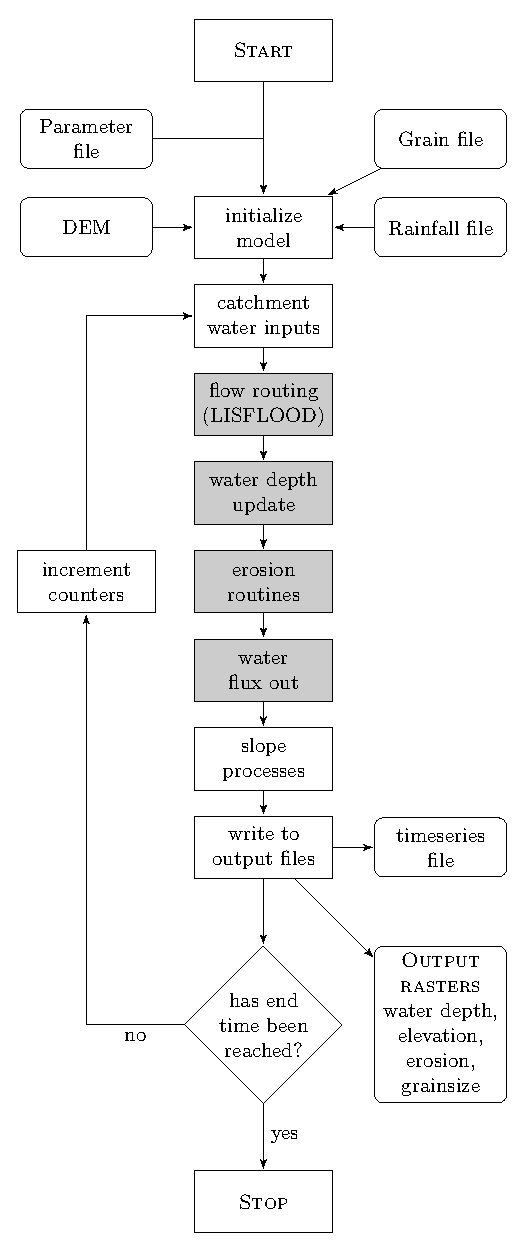
\includegraphics[width=8.3cm]{chp05_figures_scripts/tikz.eps}
\caption{Flow chart showing a simplified outline of the HAIL-CAESAR program flow. Grey shaded boxes indicate sections of the code parallelised with OpenMP. Rounded rectangles indicate output and input files.}
\label{fig_flowchart}
\end{figure}

\subsection{Potential speed up from parallelisation}

The functions described above, \textit{flow\_route, depth\_update, scan\_area,} and \textit{erode}, account for 98\% and 94\% of the compute-time in hydrology-only and erosion-enabled modes, respectively. The model is profiled using a 48 hour test simulation of a flash flood event in the summer of 2004 in the UK, referred to as the `Boscastle' simulation. (Full details of this flood event are described in Chapter \ref{chapter_events}.) Effective parallelisation of the compute-time dominating functions should result in effective parallel speed-up. The potential speed-up as a result of parallelisation can be estimated using Amdahl's law \citep{amdahl1967validity}. The law gives the predicted speed up on \(N\) processing units based on ideal scaling over multiple cores. Ideal parallel speed-up, \(S\) is given by:

\begin{equation}
S = \frac{1}{(1-P)+(P/N)}
\label{eqn_amdahl}
\end{equation}

\noindent
where \(P\) is the proportion of program time that can be run in parallel. (Note that \(P\) may vary slightly between simulations, based on the input data and certain model parameters supplied to the program.) Profiling the program with the Intel VTune amplifier performance analysis tool suggests that the program spends 94\% of its time in parallel sections of the code during an erosion-enabled simulation and 98\% of compute-time in parallel sections during a hydrology-only simulation. Using Amdahl's law it is possible to calculate theoretical potential speed-up given in Table \ref{Amdahl_table}. At the maximum available processor count of 48 cores, speed ups of up to c.20 times are predicted for a hydrology-only simulation, and up to c.13 times for an erosion-enabled simulation. The limitations of Amdahl's law are that it predicts only idealised speed ups, and does not account for any overheads in parallelisation, such as the creation and synchronisation of threads, nor does it account for performance issues due to the speed of memory access in memory-bound computational problems \citep{hill2008amdahl,sun2010reevaluating}.

\begin{table}
\caption{Idealised potential speed-up according to Amdahl's law (equation \ref{eqn_amdahl}). Value for \(P\) calculated using profiling results from the River Valency flood test simulation after 48 hours simulated time.}
\begin{tabular}{ccc}
%\multicolumn{3}{c}{\textbf{Idealised parallel speed-up}} \\ 
\textbf{Number of CPUs} & \textbf{Speed-up} (Hydro) & \textbf{Speed-up} (Erosion) \\

 & \(P=0.98\) & \(P=0.94\) \\
\hline 
2 & 1.94 & 1.89  \\ 
4 & 3.67 & 3.39  \\ 
8 & 6.11 &5.63  \\ 
16 & 11.03 & 8.42 \\ 
32 & 16.58 & 11.2 \\ 
48 & 19.92 & 13.4 \\ 
\hline \\
\end{tabular}

\label{Amdahl_table} 
\end{table}



\section{Testing and benchmarking}

\subsection{Regression testing}

Regression testing is a software development practice used to verify that software that has been modified, interfaced with other software, or re-implemented, still performs as expected when compared to the original implementation \citep{wong1997study}. To verify that HAIL-CAESAR produces comparable results to the original CAESAR-Lisflood model, a set of simulations with the same test data and input parameters for both implementations is carried out. The catchment hydrological and sediment outputs from a 10-year simulation of the River Swale, North Yorkshire, United Kingdom are compared for consistency between both implementations. The Swaledale test case has been well calibrated in previous studies \citep[e.g.,][]{Coulthard2001} and is supplied with the original CAESAR-Lisflood model as a standard test case. Details of the model testing simulations are shown in Table \ref{versus_CL}. The HAIL-CAESAR model is tested with two different compilers, to assess any potential differences arising from the choice of compiler. Three metrics are used to compare the two implementations: water discharge rate from the catchment outlet, hourly sediment output, and cumulative sediment output from the catchment over the course of the simulation. 
Figure \ref{fig_swale_regression_lisflood} shows the differences in water discharge comparing HAIL-CAESAR with the original CAESAR-Lisflood model. (For clarity, only the first 250 days are shown.) The flow routing algorithm performs similarly in both models, with the largest discrepancies seen in the first 100 days. An inset in Figure \ref{fig_swale_regression_lisflood} shows the typical magnitude and timing of differences in the discharge. The timing and magnitude of the largest flood peaks are comparable, and the largest differences in magnitude on the order of 1--10 \(m^3s^{-1}\).
Figure \ref{fig_swale_regression_sediment} shows the sediment flux from the catchment outlet. While there is low-magnitude variation in the sediment flux signal, the main peaks in sediment discharge are at similar times and of similar magnitude in both implementations. Figure \ref{fig_swale_regression_cum_sediment} shows the cumulative sediment output from the catchment. Initially, both implementations show close agreement, until approximately 700 days into the test simulation where the predicted sediment totals begin to diverge. The CAESAR-Lisflood implementation, in this case, predicts an overall lower total sediment discharge over the 10-year period. The HAIL-CAESAR implementation predicts c. 40\% greater total sediment yields after 10 years. 

\begin{figure*}[t]
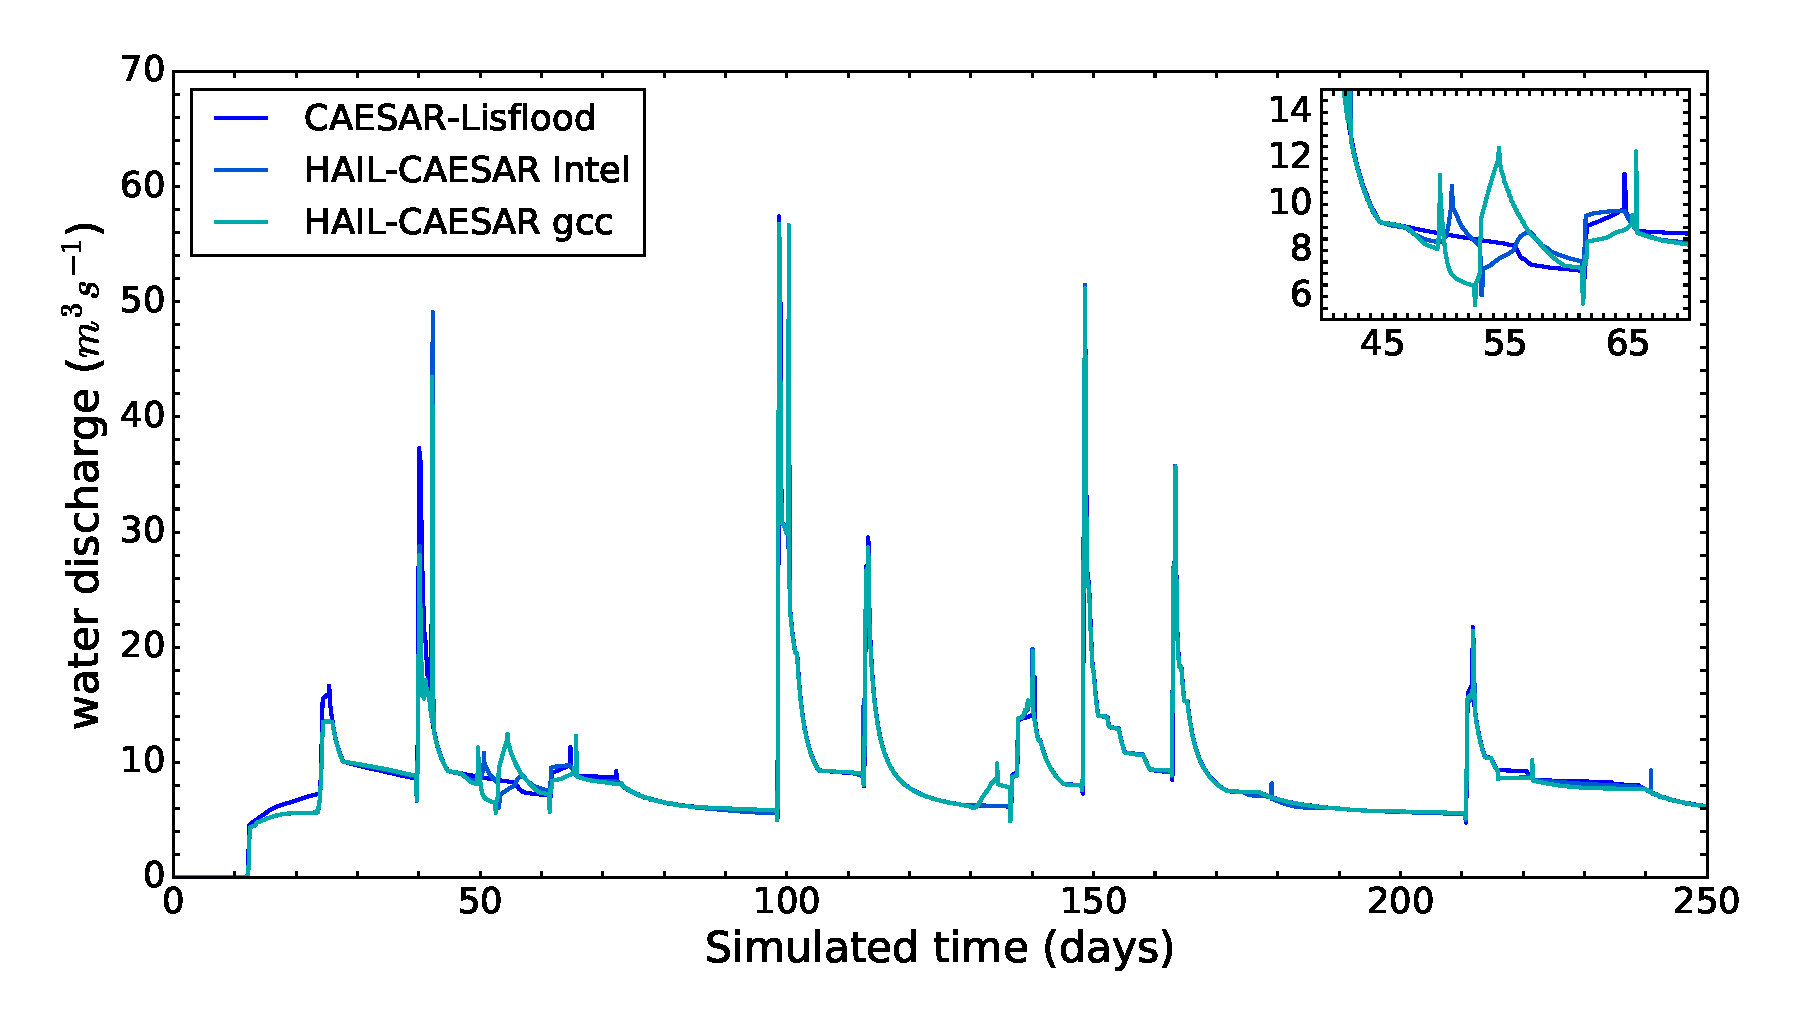
\includegraphics[width=15cm]{chp05_figures_scripts/lisflood_comparison.eps}
\caption{Water discharge rates over first 250 days of simulation. Outputs from the Swale 10 year at 50m resolution test case, showing results from the original CAESAR-Lisflood model and HAIL-CAESAR model compiled under two different compilers.}
\label{fig_swale_regression_lisflood}
\end{figure*}

\begin{figure*}[t]
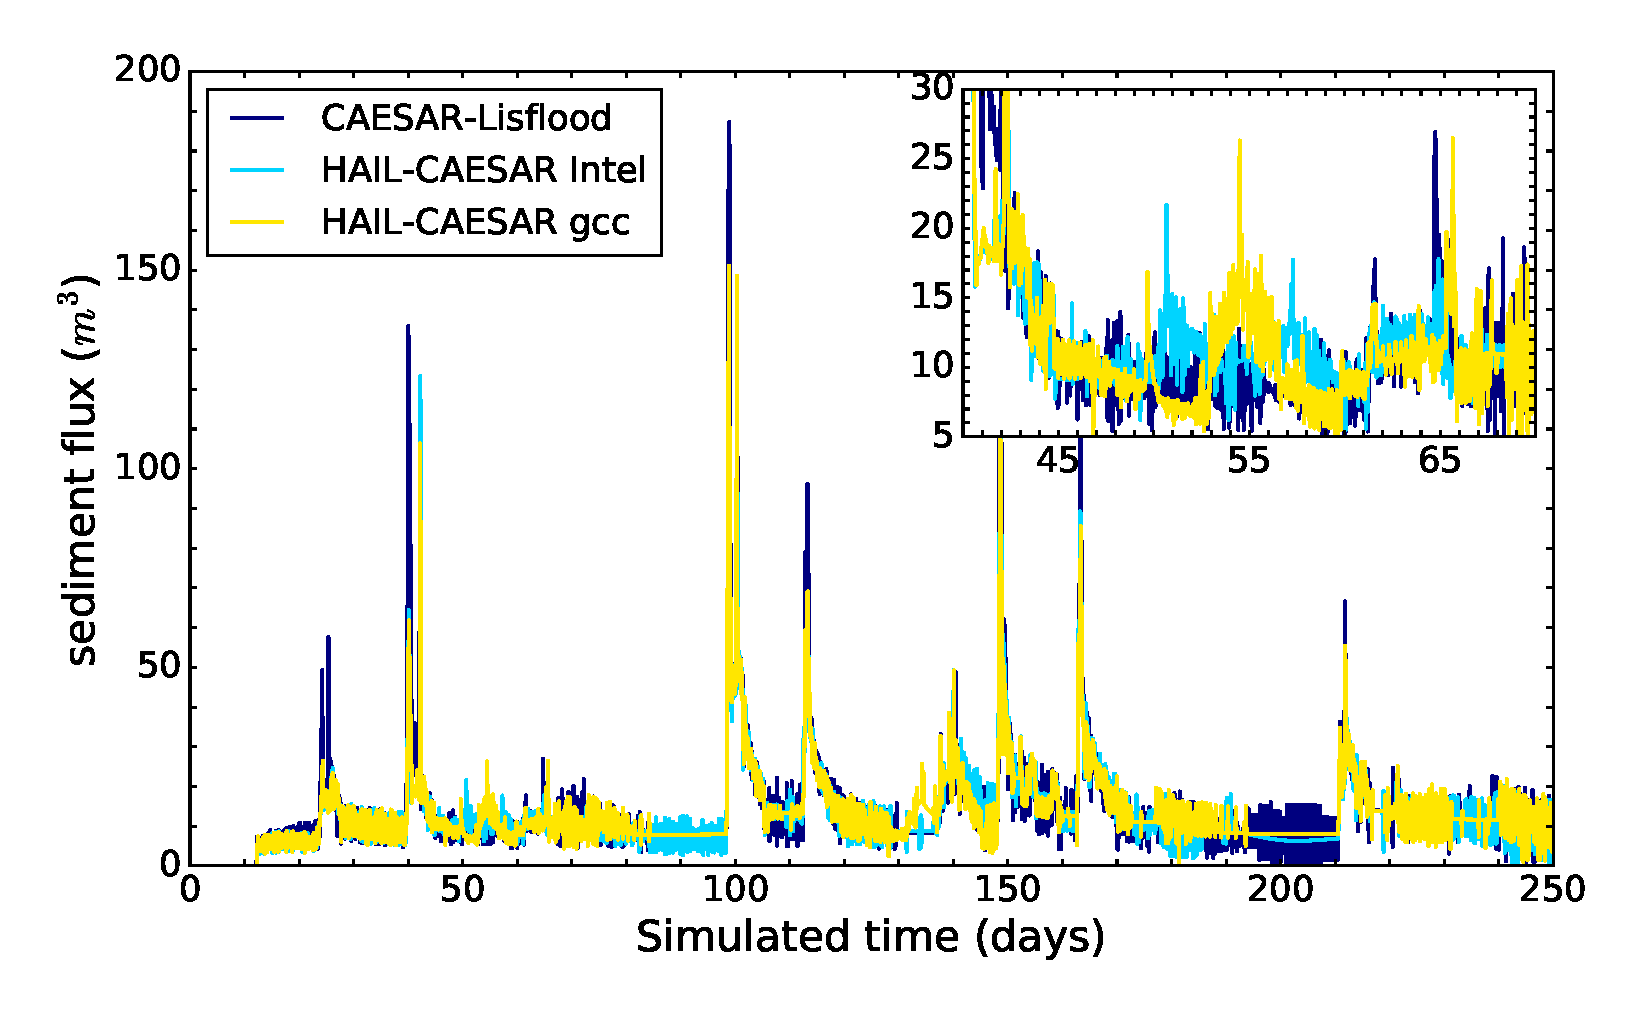
\includegraphics[width=15cm]{chp05_figures_scripts/sed_tot_comparison.eps}
\caption{Catchment sediment flux over first 250 days of simulation. Outputs from the Swale 10 year at 50 m resolution DEM test case, showing results from the original CAESAR-Lisflood model and HAIL-CAESAR model compiled under two different compilers.}
\label{fig_swale_regression_sediment}
\end{figure*}

\begin{figure}[t]
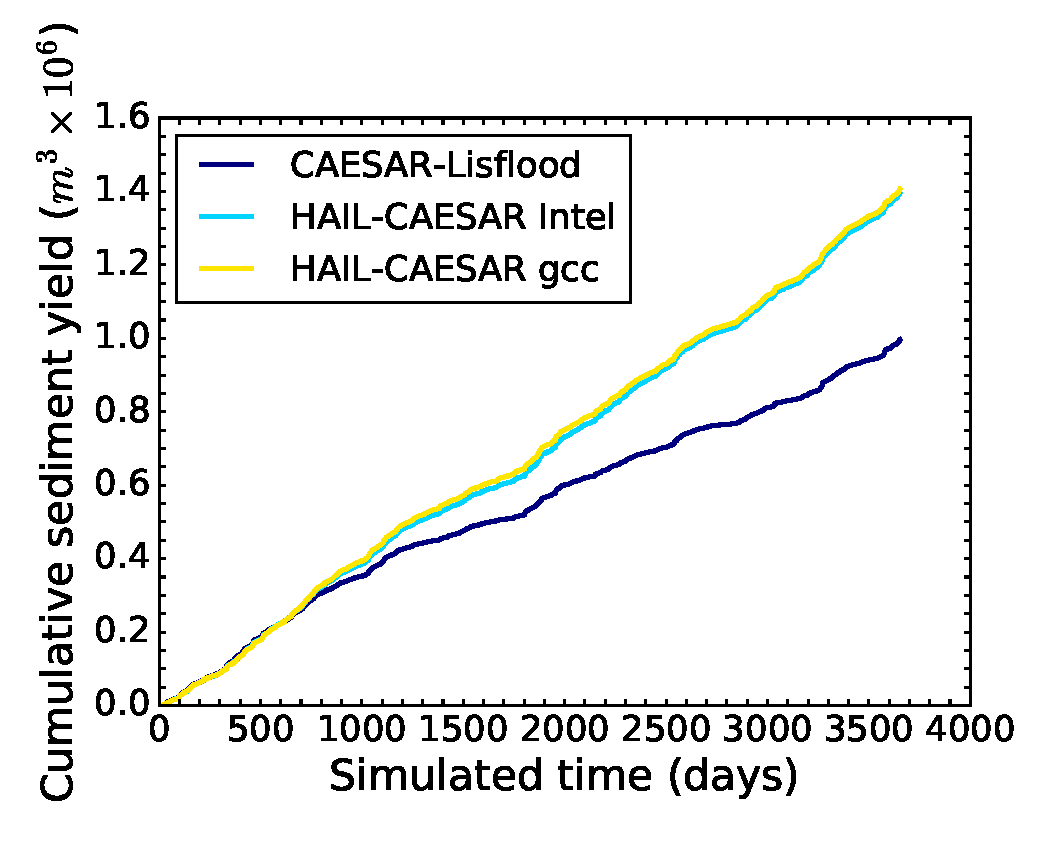
\includegraphics[width=11cm]{chp05_figures_scripts/cum_sed_tot_regression.eps}
\caption{Cumulative catchment sediment flux over full duration of simulation. Outputs from the Swale 10 year at 50 m DEM resolution test case, showing results from the original CAESAR-Lisflood model and HAIL-CAESAR model compiled under two different compilers.}
\label{fig_swale_regression_cum_sediment}
\end{figure}

\subsection{Performance comparison with CAESAR-Lisflood}

Though the code base of HAIL-CAESAR and CAESAR-Lisflood differ somewhat, due to differences in implementation detail between the C\# and C++ languages, as well as the parallelisation libraries used, the underlying algorithms remain broadly the same. The two models were compared on similar hardware to assess any gains in speed-up from porting the CAESAR-Lisflood model to a C++ implementation using the OpenMP parallelisation libraries.

The hardware used for this test study was a workstation computer with an Intel i7 8-core processor and 32GiB of memory. The CAESAR-Lisflood test simulations were run on a Windows operating system, as per the requirements of the software; the HAIL-CAESAR model test simulations were run on a Linux operating system on the same machine. The input parameters and input DEM were kept the same for all benchmarking simulations. The details of the test case configurations are shown in Table \ref{versus_CL}.

Using the HAIL-CAESAR implementation, a speed up of c.41\% was seen using the open-source GNU C++ compiler (g++) and a speed-up of 48\% using the Intel C++ compiler. As the core algorithms remain the same in both versions of the code, the speed up likely comes from the fewer overheads in the command-line based HAIL-CAESAR model, and potentially through better compiler optimisations available with the C++ compilers. Further speed up may come from the fact that the CAESAR-Lisflood model is executed through a \textit{just-in-time} compiler, translating pre-compiled bytecode into machine code at runtime \citep{aycock2003brief}. In contrast, HAIL-CAESAR runs using a compiled binary executable file, with machine code generated at compile time. The HAIL-CAESAR approach avoids the potential overheads of invoking the dynamic compilation stage in C\#/.NET programs.

\begin{table*}


\resizebox{\textwidth}{!}
{%
\begin{tabular}{cccc}
%\multicolumn{4}{c}{} \\
Model Version & \textbf{CAESAR-Lisflood 1.9b} & \multicolumn{2}{c}{\textbf{HAIL-CAESAR v1.0}} \\
\hline \\
Runtime (hrs:mins) & 7:00 & 4:09 & 3:39 \\
Programming Language & C\# & C++ & C++ \\
Compiler & MSVC 14.0 & GCC 6.2 & Intel v17.0 \\
Optimisation flags & -optimize & -O3, -march=native & -O3, -march=native \\
Parallel library & C\# native parallel library & OpenMP 4.5 & OpenMP 4.0 \\
Processor & \multicolumn{3}{c}{Intel i7-3770 8 core @ 3.4GHz, 32GiB memory} \\
\hline \\
\end{tabular} 
}
\caption{Initial performance and compilation comparison with CAESAR-Lisflood, using the River Swale test case, 50m DEM, 10 year simulation} 
\label{versus_CL}
\end{table*}

\subsection{HPC profiling and speed-up}

\subsection{Performance scaling on HPC compute nodes}
Our primary aim in developing this software was to have a code that ran on Unix-based high performance computing systems and could be re-compiled for a variety of different platforms and computer architectures. This section demonstrates the scaling potential and optimal hardware configurations using a single compute node on a typical HPC system. Test simulations are run on the ARCHER supercomputer. Each compute node consists of a two Intel Ivybridge Xeon processors, each with 12 cores per physical processor. Simultaneous multi-threading allows each core on the processor to effectively act as if it were two separate processing units, giving a total of 48 possible threads/cores per compute node. A single compute node consists of two NUMA\footnote{Non-uniform memory access}-regions each with access to 16GiB of memory, a total of 32GiB per compute node. 

\subsection{Strong scaling}
Strong scaling describes how the performance increase of the code scales as more processors are used to solve a problem of fixed size. We test two typical use case scenarios for the HAIL-CAESAR model. The first case is an extension of the standard test case using the Swale data. The use of the model in this case is typical of longer duration landscape evolution simulations, with periods of predominantly low hydrological flows interspersed with brief (relative to the simulation time) storm events. The second case uses the HAIL-CAESAR model to simulate a single storm event at higher spatial resolutions, over a much shorter timescale. Two contrasting model applications are chosen to represent the range of timescales the model can be applied to, from short term single storm events to annual and decadal simulations. 

\begin{table}
\caption{Strong scaling test cases used to benchmark the HAIL-CAESAR model, using Swaledale and Boscastle DEMs.}
\begin{tabular}{ccccc}
\\
\multicolumn{5}{c}{\textbf{Strong scaling benchmarking simulations}} \\
\hline 
Catchment & Swaledale & \multicolumn{3}{c}{Boscastle} \\
Grid cells & 124931 & \multicolumn{2}{c}{720000} & 4500000 \\ 
DEM cell size & 50m & 5m & 5m & 2m \\ 
Simulation time & 8670 hrs & 48 hrs & 72 hrs & 72 hrs \\ 
Catchment Size & 150km$^2$ & {12km$^2$} & {12km$^2$} & {12km$^2$} \\ 
Number of cores & \multicolumn{4}{c}{1, 2, 4, 8, 16, 20, 30, 36, 40, 48} \\ 
\hline \\
\end{tabular} 
\label{strong_scale_table}
\end{table}

\paragraph*{Multi-event simulation, 1 year}
The Swaledale test case is run over a 1 year duration, using an input DEM of 50 m resolution. The model is run in hydrology-only and erosion-enabled modes. The input parameters and input DEM are the same for each simulation, as each simulation is repeated on an increasing number of processors (Table \ref{strong_scale_table}). At the maximum core count of 48 core, results from this simulation show speed up of up to 700\% and 550\%, for erosion-enabled and hydrology-only modes, respectively. The speed-up shown for erosion-enabled simulations does not always increase in concert as core-counts are increased, although the overall trend is one of increasing speed-up. For example, erosion-enabled simulations with 16, 24, and 36 processors showed a slow down when compared to the preceding benchmark tests using 12, 20, and 30 processors, respectively (Figure \ref{fig_strong_scale_multi}). The hydrological-only simulations showed a more consistent speed-up between benchmark tests (Fig. \ref{fig_strong_scale_multi}), though speed-up potential begins to decline at thread counts around 30 threads and higher, where it is observed the gains from increasing the thread count further diminish.

\paragraph*{Single-event simulation, 48--72 hours}

For this benchmark, two sets of strong scaling experiments are done with two different resolution DEMs. For each set of experiments, the input terrain data and parameters remain the same while increasing the number of processors over which the problem is shared. The strong scaling benchmark tests use a model domain with a) 720 000 grid cells, and b) 4 500 000 grid cells, representing a 12km$^2$ river catchment with 5m and 2m resolution DEMs, respectively. At this resolution of DEM, it possible to resolve the larger channel geometries at the grid-scale, without resorting to techniques of `burning in' the DEM with a channel. Sub-grid parameterisation of the channel shape, a feature of some models, is also not required.

Since HAIL-CAESAR features both a flood-inundation-only and sediment erosion mode, two further sets of benchmarks were done for both problem sizes, one with the model running in hydrology-only mode, and another running in the erosion-enabled mode.

The results from the single-event scaling benchmark show the greatest speed-up for the 48 hour Boscastle simulation, with a speed-up of almost 16 times at 48 threads/cores, for the hydrology-only simulation. Erosion-enabled simulations also show food speed-up for this problem size (720 000 grid cells), but the linear speed-up trend is lost above around 30 cores, when speed-up gains begin to tail-off. At the larger problem size of 4 500 000 grid cells, the speed-up gains from increasing core counts is much diminished, though still increases linearly through higher core counts. Speed-up here reaches only about 5 times running on 48 cores, in hydrology-only mode, and 3.5 times in erosion-enabled mode.

\begin{figure}[t]
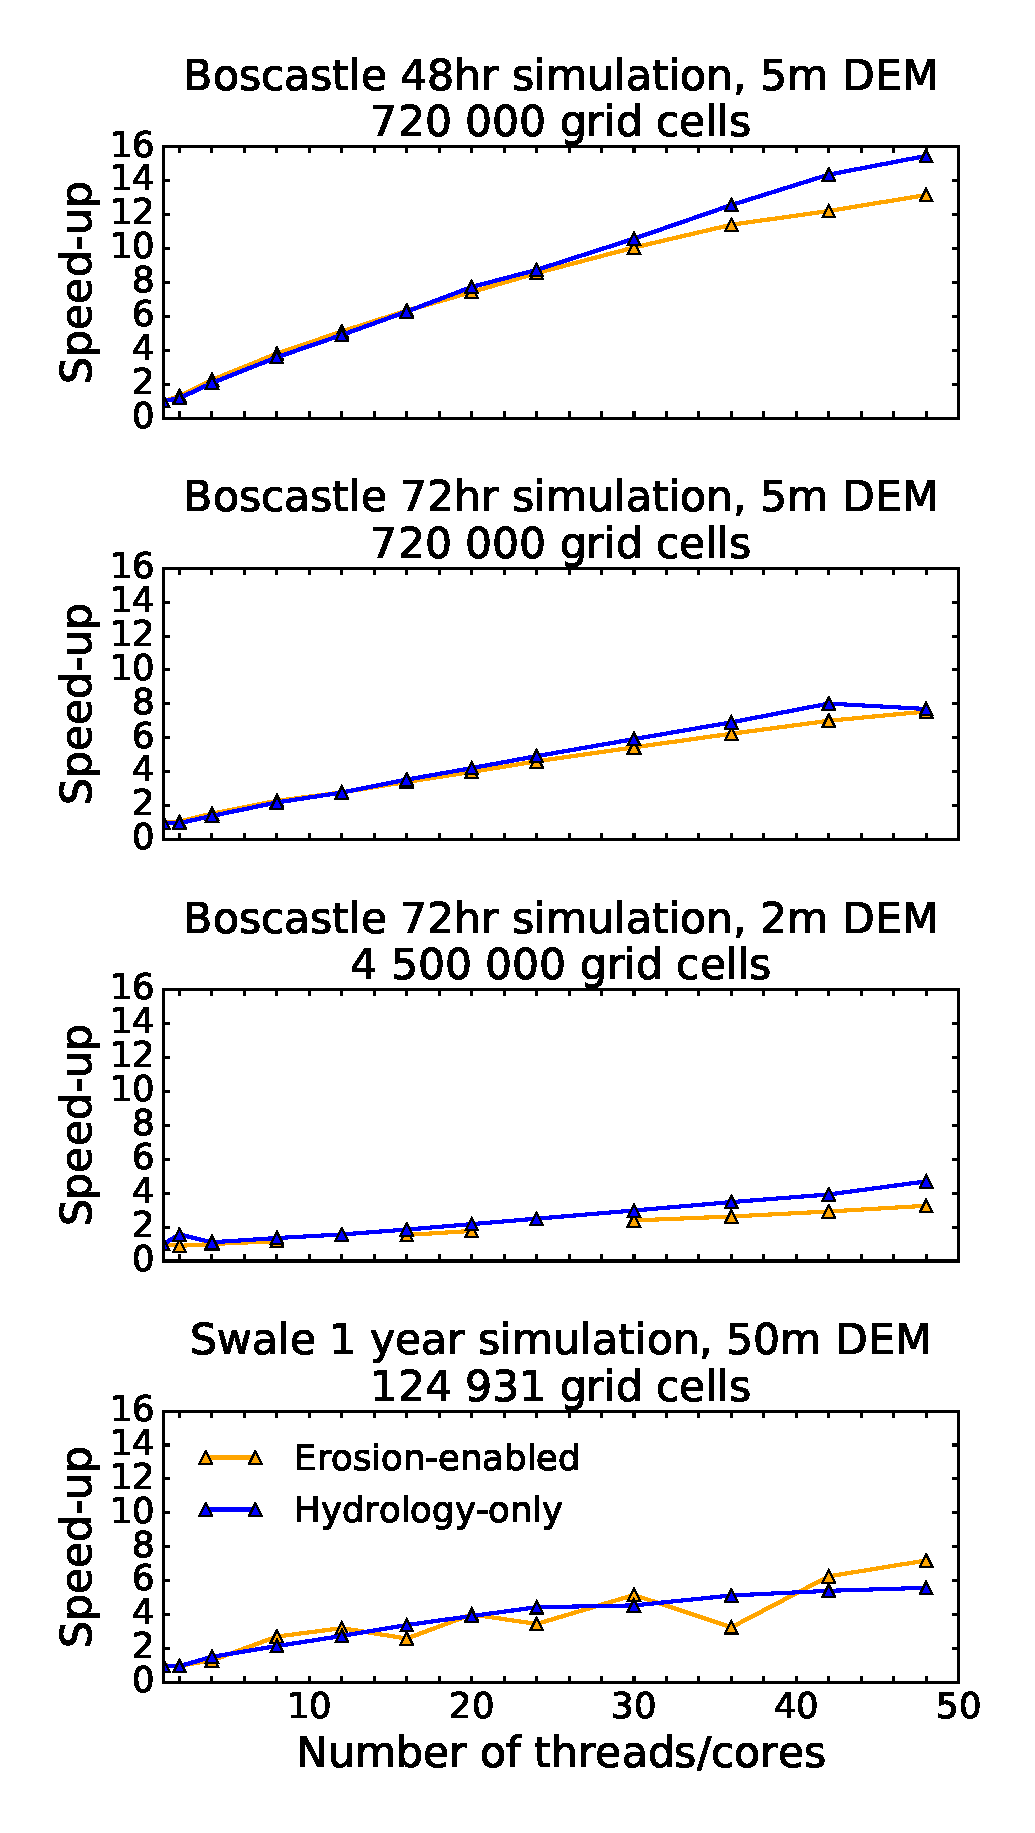
\includegraphics[width=11cm]{chp05_figures_scripts/strong_scale_four.eps}
\caption{Speed-up achieved relative to serial code on 2, 4, 8, 12, 16, 20, 24, 30, 36, 42, and 48 cores. Four sets of simulations are used representing a range of model uses from short, single event episodes (48--72hr) to 1 year simulations.}
\label{fig_strong_scale_multi}
\end{figure}

\subsection{Weak scaling}

Weak scaling is a parallel performance metric used to assess how the code runtime scales as the amount of work per processor is kept the same, but the total problem size -- in our case, the number of grid cells in the model domain -- is increased \citep{gustafson1988reevaluating}. This mirrors the practice of using larger numbers of processors to tackle model simulations using higher resolution topographic data, or data covering a larger spatial domain. The weak scaling experiments used a set of hydrology-only simulations and a set of erosion-enabled simulations. A series of 72 hour simulations were done using a range of high-resolution topographic datasets, from 0.5 m to 5 m resolution, scaling the number of processors used to maintain the ratio of processors/workload as near as possible. The number of model domain grid cells per core was fixed at approximately 1 500 000. The simulations were repeated for hydrological-mode and erosion-enabled modes, but due to the high memory demands of running very high resolution erosion-enabled simulations, not all simulations could be completed on the available hardware, which has a maximum job runtime of 48 hours.

The simulations in hydrological-only mode show positive weak scaling as the problem size increases in tandem with the number of threads (Figure \ref{fig_weak_scale}). Ideal weak scaling would be expected to show a runtime per number of grid cells/cores remaining approximately constant compared with a single-threaded simulation. The slight increase seen in the weak scaling here is likely due to the overheads experienced with creating and synchronising the extra threads as the problem size is increased.

\begin{sidewaystable*}[t]
\caption{Weak scaling test cases with the Boscastle DEM resampled at increasing resolutions from 0.5m to 5m. The absence of run-time results for certain erosion simulations is due to memory limitations preventing higher resolution simulations from running.}
\resizebox{\textwidth}{!}
{%
\begin{tabular}{ccccccc}

\multicolumn{7}{c}{\textbf{Weak scaling simulations, Boscastle DEM, 72 hour simulation}} \\ 

DEM resolution (m)  &  Grid cells & Ideal no. of threads & No. of threads & Cells per thread & Run time (Hydro) & Run time (Erosion) \\ 
\hline
0.5 & 72 000 000 & 48    & 48 &  1 500 000 & 323.1 & --  \\
0.6 & 49 900 050 & 33.3 & 33 &  1 512 122 & 190.4 & -- \\
0.7 & 36 808 200 & 24.5 & 26 &  1 472 328 & 138.8 & -- \\
1.0 & 18 000 000 & 12    & 12 &  1 500 000 & 84.3 & 355.2 \\
1.5 & 7 960 050   & 5.3   &  5  &   1 592 010 & 49.0 & -- \\
2.0 & 4 500 000   & 3      &  3  &   1 500 000 & 568.9 & 1112.1 \\
5.0 & 720 000      & 0.48 & 1  &    720 000 & 347.306 & 432.3 \\ 
\hline \\
\end{tabular} 
}
\label{weak_scale_table}
\end{sidewaystable*}

\begin{figure}[t]
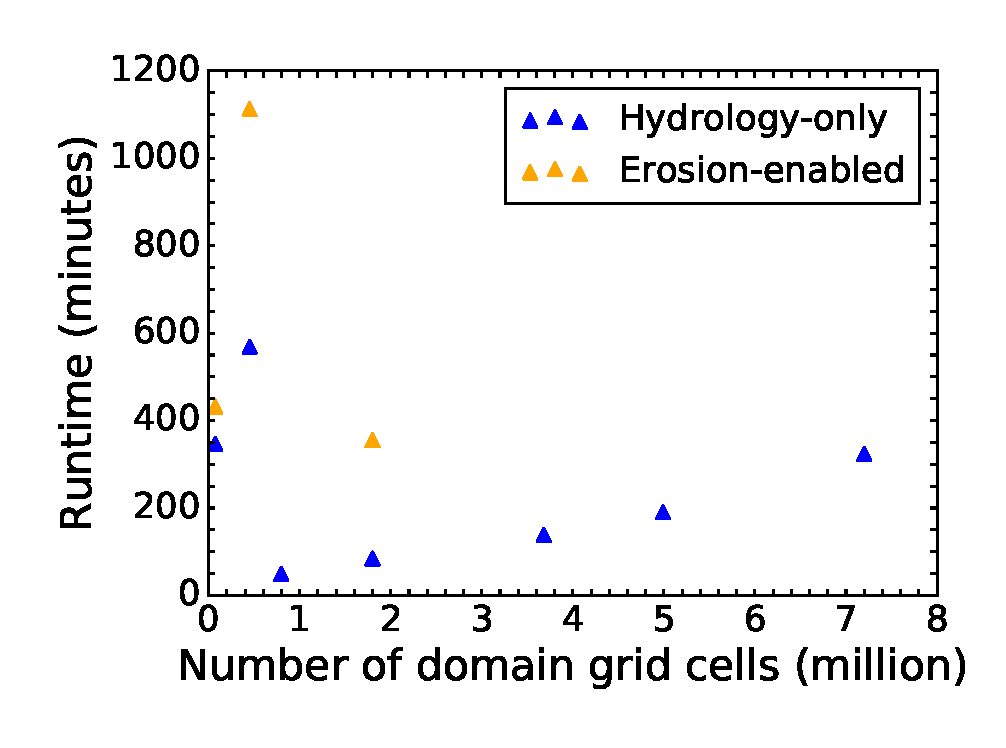
\includegraphics[width=11cm]{chp05_figures_scripts/weak_scale_bos.eps}
\caption{Weak scaling with the Boscastle DEM at increasing resolution (see Table \ref{weak_scale_table}). Hydrological and erosion-enabled simulations shown. Each simulation uses c.150 000 grid cells per CPU. The absence of results for certain erosion simulations is due to memory limitations preventing higher resolution simulations from running.}
\label{fig_weak_scale}
\end{figure}


%\subsubsection{Compiler influence}
%
%The influence of compiler choice on performance is investigated using three compilers: gcc v5.1, Intel vX, and the Cray compiler vX.X.
%
%\subsubsection{Optimisation options}

\subsection{Thread profiling}

Further profiling of the parallelised version of the code was carried out using the Intel\textregistered \ VTune Amplifier performance analyser. Thread profiling allows us to see where the bottlenecks in the code are, including functions that are compute intensive, but also where inefficiencies occur due to overheads from parallelisation and load imbalance. For clarity, a single example using the Boscastle test case is presented, with a simulated model time of 48 hours, running on 8 cores/threads. It is expected that different simulations and domain sizes would produce slightly different results, but this simulation gives a general idea of the parallel performance of specific functions in the code.

The break down of major function overheads is shown in Figure \ref{fig_thread_profile}. Only four of the key parallel-implemented functions, \textit{erode, flow\_route, scan\_area,} and \textit{depth\_update} are assessed, as other functions collectively amounted to a small proportion of the runtime, or were serial functions. Load imbalance accounts for 22\% of the execution time of these four key functions, due to certain threads sitting idle while waiting for other threads to complete. Load imbalance is particularly apparent in the \textit{erode} and \textit{depth\_update} functions. Overhead time (from the creation and synchronisation of threads) is minimal across all functions. The issue of load imbalance is discussed further in Section \ref{sec_loadbalance}.

\begin{figure}[t]
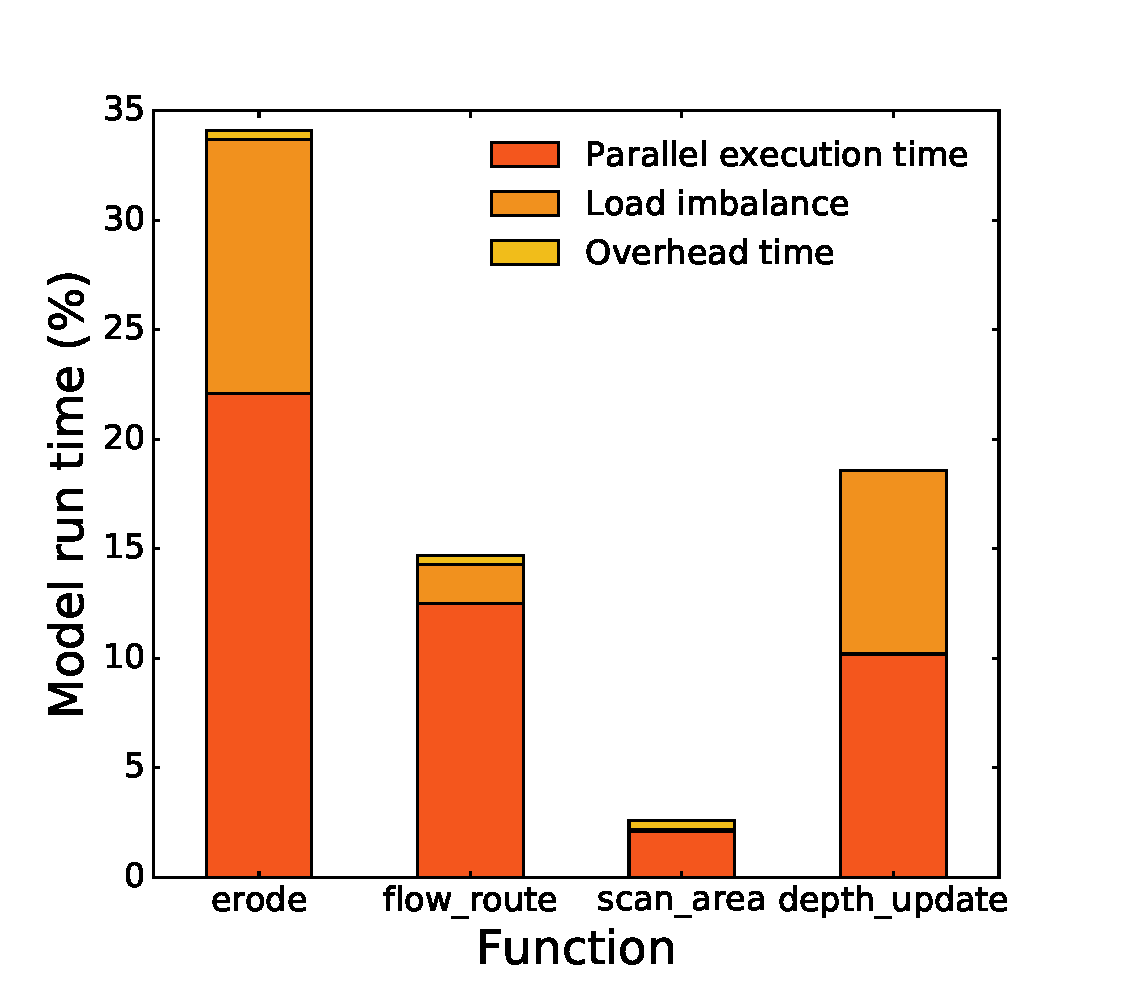
\includegraphics[width=11cm]{chp05_figures_scripts/fig_thread_profile.eps}
\caption{Thread profiling of the Swale 1 year simulation with 50m DEM. Data from major functions only displayed.}
\label{fig_thread_profile}
\end{figure}

%\subsection{Ensemble simulation potential on HPC clusters}
%
%The growing availability of HPC services has been thus far seldom exploited by the geomorphic and landscape evolution modelling community. This section briefly explores the potential for using such computing services to run ensemble simulations of landscape evolution models, using the HAIL-CAESAR model and Swale test case used in previous sections. The ARCHER HPC service is used for the test simulations. 

\section{Discussion}

%Strong scaling
%weak scaling
%Problem-type and size dependency
%Load-balancing issue
%Scheduling

\subsection{Parallel scaling}
%Strong scaling
%weak scaling
%Problem-type and size dependency
There are three factors that potentially affect the parallel scaling observed in the benchmarking test cases presented. 
\begin{enumerate}
\item The number of grid cells in a model domain, i.e. the total problem size, which is dependent on the resolution of the DEM input data. 
\item The choice of running the simulation as hydrology-only or erosion-enabled model. The erosion option in the model also increases memory demands significantly compared to the hydrology-only mode, as well as computational expense.
\item The hydrological state of the catchment. When the catchment is experiencing flooding due to high rates of rainfall input, the number of cells registered as containing water through the \textit{scan\_area} algorithm increases substantially. The location of the water-containing cells in a catchment also determines the amount of load-imbalance in the model. If water-containing cells are concentrated only in a certain area of the catchment, significant load-imbalance will occur. 
\end{enumerate}

The most favourable speed-up was observed in the Boscastle 48 hour simulation at 5 m DEM resolution (Figure \ref{fig_strong_scale_multi}.) A speed-up of almost 16x was recorded using the maximum number of cores available on the test hardware. Increasing the length and resolution of the Boscastle simulation appeared to negatively affect the speed-up potential of the simulation. Speed-up gains remained approximately linear into higher core counts, with slight tail-off in speed-up gains observed when approaching 48 cores. The longer-term Swale simulation exhibited poorer scaling, with a gradual drop in speed-up gains as the number of threads/cores was increased. 

There is not a clear relationship between number of grid cells in the model domain and speed-up potential. The Swale test case (about 125 000 grid cells), for example, showed almost half as much speed up as the 48 hour Boscastle simulation, despite the latter having 720 000 grid cells in the model domain. 

The enabling of erosional processes in simulations did not significantly affect the scaling potential of the simulations. Most benchmark results showed slightly less favourable speed up at higher core counts for erosion-enabled simulations, but this did not appear to be the controlling factor on scaling. In one case (Swale) the erosion-enabled simulation ran 2x faster than the corresponding hydrology-only simulation. The lack of contrast between erosion-enabled and hydrology-only simulations may be explained by the adpative time stepping feature used in the \textit{erode} function. In erosion-enabled mode, the timestep increases substantially during periods of low water flow and erosion rates, and this may offset the increased computational demands from the \textit{erode} function.

The Boscastle and Swale test cases represent different types of catchment hydrological state. The Boscastle simulations essentially represent a single intense flooding event, where the catchment is in a period of low flow followed by an intense burst of rainfall and erosion for a few hours. The Swale simulation represents a series of storm events, interspersed with `dry' periods, where the model will be able to increase the timestep, but not make heavy use of parallel sections of the code reserved for water routing and erosion routines. 

\subsection{Load balancing issues}
\label{sec_loadbalance}
Parallel computing problems in which the distribution of workload between each thread or processor is uneven are said to suffer from \textit{load-imbalance}. In other words, although the model domain is divided into equally sized chunks for the number of threads and processors available, each thread will not necessarily receive an equal amount of work to do \citep{sakellariou1996quest}. Threads with little amounts of work to do will therefore remain idle while waiting for  heavily-loaded threads complete their assigned work. Numerical simulation of river catchments is inherently load-imbalanced. The load balance problem arises from the nature of catchment processes, where the most rapid rates of geomorphological activity occur in river channels. In river channels, rates of water flow and sediment transport are greatest, relative to the processes operating on hillslopes. The inherent heterogeneity in the nature of catchment processes translates into computational imbalance during model simulations of river catchments. Within the model domain representing a catchment, the grid cells of the domain representing river channel sections will make the greatest computational demand, due to repeated calls to subroutines that calculation or update cell properties. Highly active river channel cells will frequently exceed thresholds set for the calculation of water flows and sediment entrainment, whereas cells representing hillslope areas will be active relatively infrequently.

The mechanism in the model that determines which cells will be updated each iteration is the scanning algorithm described in the \textit{scan\_area} section. The algorithm was originally designed \citep{Coulthard2013} to substantially reduce the number of cells in the model domain that had to be updated each iteration, by isolating the cells that contain water and only performing erosion and sediment transport routines on those `wetted' cells. While the algorithm is effective at reducing compute time this way, it creates a load-imbalance problem for parallel implementations as the location of computationally intensive areas of the model domain cannot be easily predetermined. While threads are assigned equal numbers of iterations, each iteration is not necessarily equally load-balanced in terms of computational expense. In algorithms that perform a global scan of all cells in the model domain, such as the parallel implementation of the flow routing algorithm in \citet{neal2009parallelisation}, load imbalance is minimalised because threads are kept occupied working on every grid cell, rather than focusing on a subset of grid cells with discharge or water depth above a given threshold, as is done in the HAIL-CAESAR model. A global scanning algorithm was initially explored in the implementation of HAIL-CAESAR, allowing the removal of the \textit{scan\_area} function, but the increase in run-time was so substantial it negated any potential improvements in load balance among the OpenMP threads. 

\subsection{Loop scheduling}

The OpenMP application programming interface (API) will automatically partition iterations of a loop between the available number of threads. By default these are assigned statically when a \texttt{parallel for} block is entered, with threads receiving an equal number of loop iterations to carry out. The default behaviour can be overridden, however, by explicitly specifying a different scheduling type for parallel for loops. For load imbalanced problems such as discussed in this paper, the \textit{dynamic} loop scheduling can improve parallel performance by reducing the amount of idle time that threads spend waiting for busy threads to complete their workload \citep{willebeek1993strategies,olivier2012openmp}. The default behaviour of the dynamic scheduling type is to assign each loop iteration to one thread, and when the thread finishes it is assigned the next iteration that has yet to be executed. Experiments in finding an ideal loop scheduling set-up to reduce load imbalance in HAIL-CAESAR showed mixed results, with no clear indication that using the dynamic scheduling clause improved run-times in all cases. However, in some test cases, dynamic loop scheduling was shown to offer performance improvement. For this reason, the HAIL-CAESAR model provides users with the option to set the loop scheduling type at run time, by specifying the \texttt{OMP\_SCHEDULE} environment variable before running the model. It is recommended that users experiment with using dynamic scheduling for their own simulations as it may offer performance increases over default scheduling.



\section{Conclusions}  %% \conclusions[modified heading if necessary]
An implementation of a hydrodynamic landscape evolution model was developed, based on the CAESAR-Lisflood model \citep{Coulthard2013}. The new C++ implementation of the model is modular, cross-platform, and scalable to multi-core computing systems through the implementation of shared-memory parallelism with the OpenMP API. Minimal code changes were required to the serial version of the code to deliver a parallel compute code. The model exhibits a performance increase of c.40\% compared to the CAESAR-Lisflood implementation in a like-for-like benchmark. The scaling potential of the model is variable, depending on the size of the problem domain and the likely hydrological state of the river catchment being simulated. In most test cases, linear speed up is achieved at moderate core counts of up to 48 cores, on model domain sizes of up to 4.5 million grid cells. Computational load imbalance was a substantial problem in the model. The causes of the load balancing issues in the model are likely due to the spatially-heterogeneous nature of catchment-scale hydrological and erosional processes. Suggestions are made for minimising load imbalance through dynamic loop scheduling, but the success of these scheduling methods is highly dependent on the input data to the model.


%=-=-=-=-=-=-=-=-=-=
% CASE STUDIES AND MODEL SET-UP
%=-=-=-=-=-=-=-=-=-=

\chapter{Model set up and parameterisation of two flash flood events in the UK}
\label{chapter_events}
\chaptermark{Severe storms in Cornwall and northern England}

\section{Background}
Intense rainfall events may be short lived, lasting only a few hours, but have the potential to cause substantial and destructive flooding \citep{lane2008climate,pitt2008pitt}. In the UK, many of these storms occur in the summer \citep{Kendon2014}, and their severity is often the result of a combination of meteorological factors. From a meteorological perspective, flash flooding can be predicted through an ingredients-based method; a systematic assessment of the key components present to cause an intense rainfall event likely to lead to flash flooding \citep{Doswell1996}. In the ingredients-based approach, flash flooding occurs when there is a combination of a high rainfall rate for an extended duration of time (usually on the order of hours). Rainfall totals are in turn related to the length of the rainfall event. Factors that lead to high rainfall intensity during an event include the forced ascent of moist air, usually associated with orographically-forced rainfall events \citep{Barros1994,Houze2012}. The duration of the event is dependent of the speed of movement and the size of the system bringing rainfall; given equal intensity rainfall rates, a large, slow moving rainfall feature will cause much higher rainfall totals in a river catchment that a fast moving, smaller feature. 

Though not essential to the `ingredients-based' method of flash flood prediction, convective-type storms are frequently associated with the type of intense rainfall that leads to flash flooding \citep{doswell1993flash}, including highly-localised flooding in the UK \citep{gray1998mesoscale,Browning2007}. In certain cases, convective rainfall events may appear stationary or `quasi-stationary' \citep{chappell1986quasi,warren2014boscastle}, leading to prolonged intense rainfall over river catchments.

The combination of these ingredients leads to river catchments being subjected to high-intensity rainfall inputs at a rate faster than a river catchment can transport or store water, leading to river flooding when rivers exceed their bankfull\footnote{The water level at which a river is at the top of its banks and any further rise would result in water moving into the flood plain.} capacity, or surface water flooding if rainfall rates are greater than infiltration rates at the surface. Antecedent conditions, such as soil-moisture content, also play a role in a catchment's ability to store water, but in cases of the most extreme rainfall events, even catchments with a high potential to store incoming rainfall or slow water flow towards rivers will be overwhelmed with the rate and volume of water input and flooding becomes inevitable.

This chapter describes two intense rainfall and flash flooding events in the UK summers of 2004 and 2005. The cause and impact of the events are described as a background to them being used as case studies in a series of numerical simulations. The series of numerical simulation experiments are designed to investigate the role of rainfall spatial resolution in hydrological and geomorphological processes during severe storms, as described in Chapter \ref{chapter_intro}. % Extension from the intro chapter?

The two events used as case studies took place in 1) the Ryedale catchment, near the town of Helmsley, North Yorkshire, 2005; and  2) the Valency catchment near the village of Boscastle, Cornwall, 2004. Both catchments experienced intense rainfall leading to extensive and damaging flash flooding \citep{golding2005boscastle,sibley2009analysis}. There were significant economic impacts for both communities, as well as geomorphological changes to the river channels and flood plains observed in the aftermath of the flooding \citep{wallingford2005flooding,wass2008investigation}.

\section{Meteorological setting}
The case studies were chosen as they represented infrequent events in each particular catchment. Because there is no commonly agreed definition of what constitutes an extreme or infrequent event \citep[e.g.][]{wilby2008climate,fowler2010detecting,jones2014objective,}, for the purpose of this study, flood events likely omly to occur approximately once in several hundred years were chosen. (The return period for the 3 hour rainfall event is given in Table \ref{table_met_setting}.) Peak river discharges for each of the case study flood events exceeded the 99th percentile for their respective catchments \citep{hannaford2004development,NRFA}.  An overview map of the catchment locations is given in Figure \ref{fig_location_map}, marked by the location of their main settlements. Table \ref{table_met_setting} summarises the key features of each catchment and its associated storm.

\begin{figure}[htb]
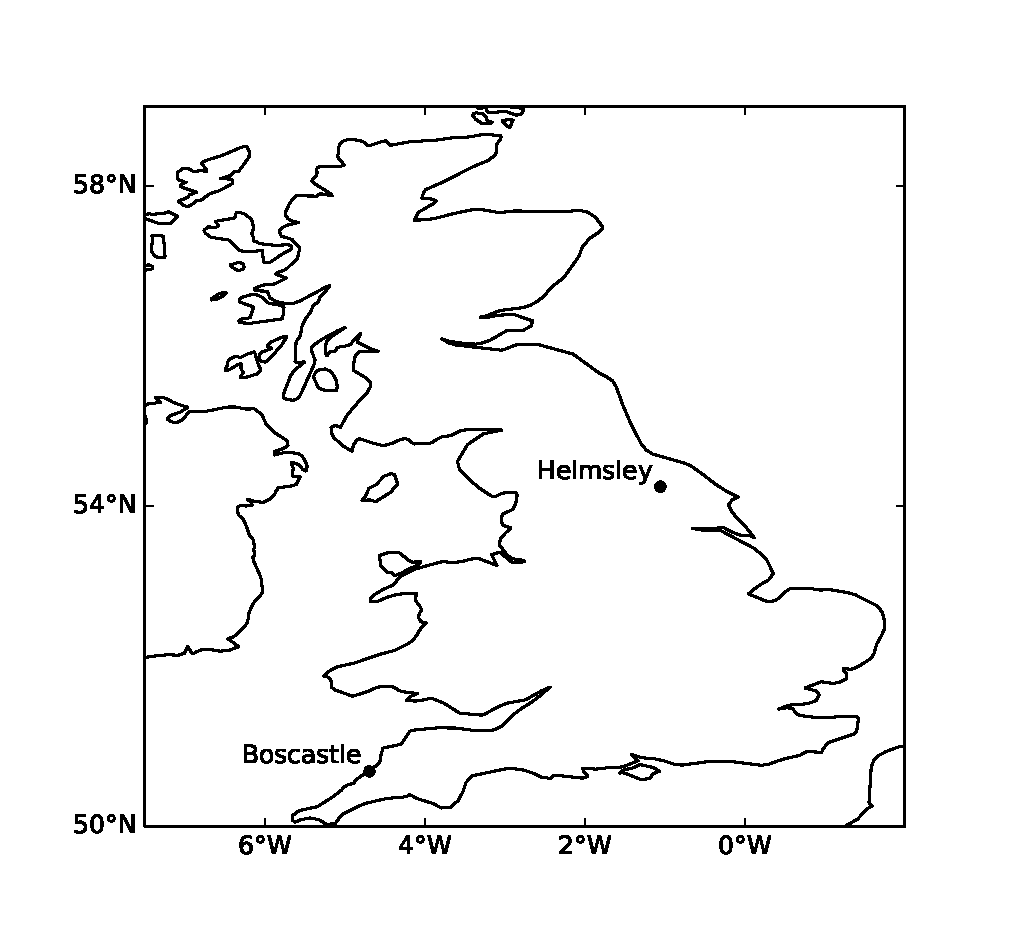
\includegraphics[width=11cm]{chp_events_figures_scripts/figure_location_map.eps}
\caption{Location of the two case study catchments in Britain, marked by the main settlement within each catchment.}
\label{fig_location_map}
\end{figure}

\linespread{1.5}
\begin{table}
\resizebox{\textwidth}{!}
{%
\begin{tabular}{l c c} \hline

Catchment Name 			& \textbf{Ryedale} &  \textbf{Valency} \\ \hline
Main settlement        & Helmsley             & Boscastle \\
Catchment Area   			& 270km$^2$ 				& 18km$^2$ \\ 
Catchment Type         & Upland, Moor/Peaty & Upland, Pasture \\ 
Storm Date	 		            & 2005-06-19 	& 2004-08-16 \\ 
Peak Rainfall	 (mm hr \(^{-1}\))  & 125  & c.400 \\
%Peak Discharge	 	 & & \\ 
Meteorological Setting	 	& Split-front, convective system & Quasi-stationary convective system \\ 
3hr Rainfall Return Period 	 & 330yr \citep{wass2008investigation}	& 1300yr \citep{burt2005cloudburst} \\ \hline
\end{tabular}
}
\caption{Table showing key characteristics of each storm event.}
\label{table_met_setting}
\end{table}

\subsection{Boscastle, Cornwall storm 2004}
The Boscastle storm took place on 16 August 2004. The storm led to flooding within the River Valency catchment and the village of Boscastle. In the preceding months March--June, the south-west area of Britain had been drier than usual, although during July the Valency catchment area experienced average rainfall conditions \citep{golding2005boscastle}. The estimated soil moisture deficit\footnote{The amount of water needed to bring the soil back to field capacity, i.e. a state where the soil is holding the maximum amount of water possible against gravity. \citep{beven2011rainfall}} in the area, which had previously been lower than average due to the dry antecedent conditions in March--June, decreased during 1--16 August, due to a return to average rainfall conditions in that month. The soil moisture deficit during this period was estimated to have decreased from approximately 80--220mm to 40--180mm \citep{golding2005boscastle}.

On the day of the storm, rainfall accumulations of up to 184mm from the Lesnewth tipping bucket raingauge \citep{golding2005boscastle} were recorded in the upper Valency catchment resulted from prolonged rainfall between 1200--1600 UTC. Rainfall rates were thought to have reached almost 400 mm hr\(^{-1}\) \citep{golding2005boscastle}, after correcting for under-reporting from rain gauges in the vicinity of the catchment \citep{burt2005cloudburst}. The rainfall accumulations from the 1km gridded composite radar product in the Valency catchment are shown in Figure \ref{fig_boscastle_rain_totals}. Note that the highest rainfall accumulations from the radar data shown in Figure \ref{fig_boscastle_rain_totals} are 115mm, lower than the raingauge totals reported in \citet{golding2005boscastle}, likely due to under reporting by precipitation radar. 

%The meteorological conditions that enabled such prolonged heavy rainfall were a combination of large-scale synoptic conditions moving in from the Atlantic, with moist lower atmospheric layers readily forming convective cloud. Repeated initiation of convection along the north Cornish coast lead to what appeared to be relative stationary convective cells over the Valency catchment. Later authors refer to this type of convective storm as a `Boscastle-type' or quasi-stationary convective storm \citep{warren2014boscastle}.

\begin{figure}[htb]
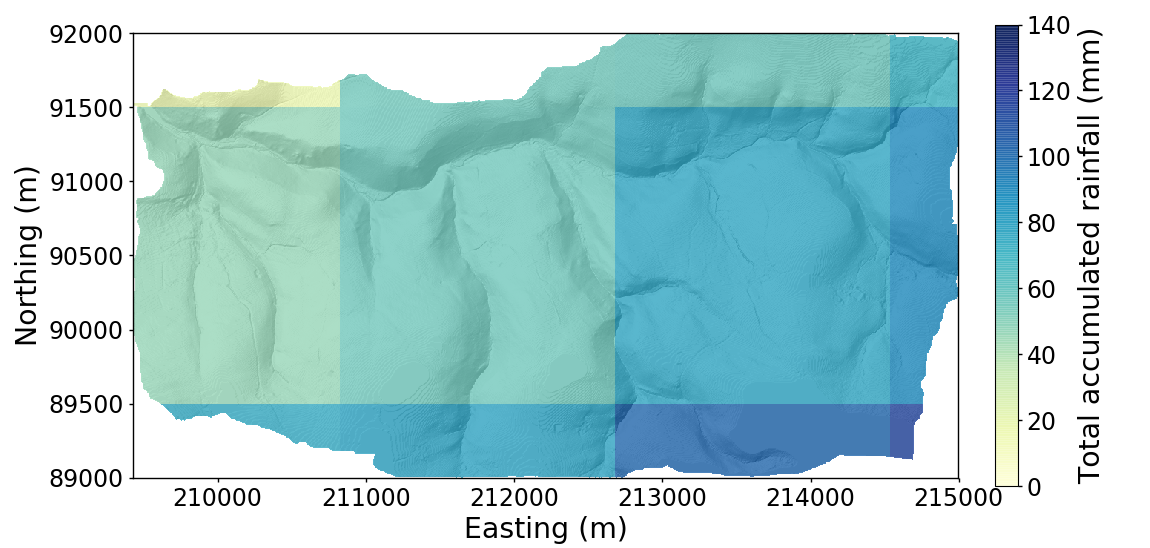
\includegraphics[width=15cm]{chp_events_figures_scripts/figure_boscastle_total_rainfall.png}
\caption{Total accumulated radar rainfall (24 hours) over the Valency (Boscastle) catchment during the 16th August 2004.}
\label{fig_boscastle_rain_totals}
\end{figure}


\subsection{Ryedale, North York Moors storm 2005}
The Ryedale storm occurred on 19 June 2005. Intense rainfall throughout the afternoon led to total accumulated rainfall amounts of up to 89mm in Ryedale between 1400--1800 UTC measured by the Helmsley raingauge. Peak instantaneous rainfall rates were estimated to have been around 32.5mm hr\(^-1\) \citep{sibley2009analysis} to 59.4 mm hr\(^{-1}\) \citep{hopkins2012knowledge}, though one report states they reached as high as 125 mm hr\(^{-1}\) \citep{cinderey2005north}. Figure \ref{fig_ryedale_rain_totals} shows the total accumulate rainfall radar totals from the 1km composite radar product. Most areas of the catchment received total rainfall accumulations similar to the reported raingauge figure (89mm), though up to 131mm is reported in one grid square in the south of the catchment area.

Antecedent conditions before the Ryedale storm of 2005 were dry over a prolonged period over much of the region \citep{sibley2009analysis}, leading to cracking of the surface peat in the higher elevations of the catchment. Soil moisture deficit was estimated to be around 60mm in the catchment, higher than usual due to the drier conditions in the preceding months \citep{wass2008investigation}. With a high soil moisture deficit, thinner soils in the upper reaches of the catchment would have been dry before the intense rainfall.

%The meteorological conditions leading to such heavy rainfall was a combination of a cold, upper-level air mass advecting over a warm moist boundary layer, leading to unstable conditions that enabled a convective thunderstorm to develop in the late afternoon. The conditions let to a particularly high amount of precipitable water present in the atmosphere which was subsequently washed out into the landscape during intense rainfall. 

\begin{figure}[htb]
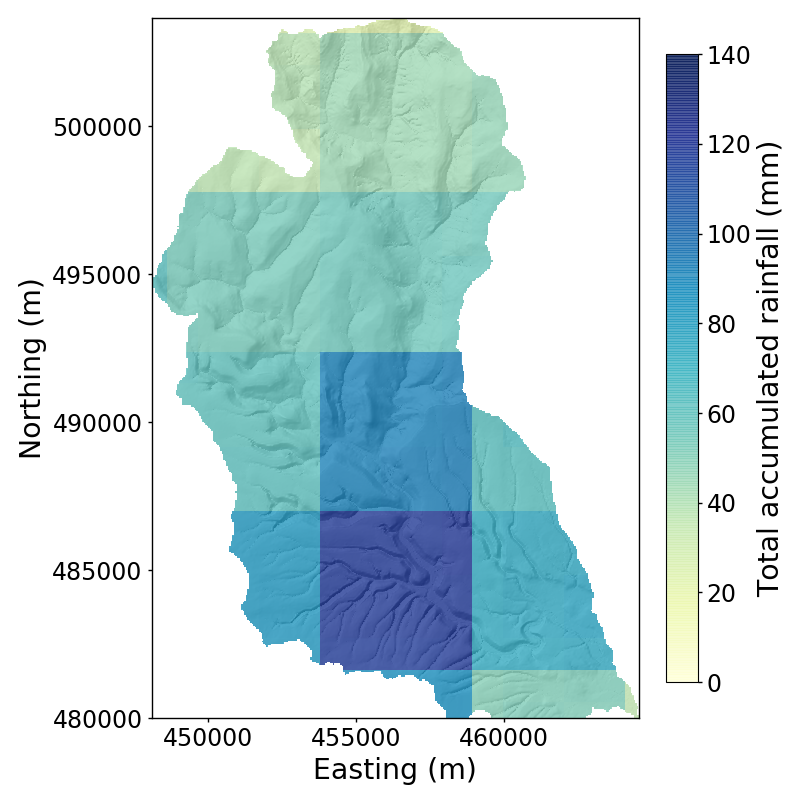
\includegraphics[width=13cm]{chp_events_figures_scripts/figure_ryedale_total_rainfall.png}
\caption{Total accumulated radar rainfall (24 hours) over the Ryedale catchment during the 19th June 2005.}
\label{fig_ryedale_rain_totals}
\end{figure}

\section{Flooding and geomorphic change}

\subsection{Boscastle, Cornwall, 2004}
Flooding was extensive in the area surrounding Boscastle village, with flood levels rapidly exceeding bankfull and flooding several properties to depths of several metres. Water levels in the Valency river and its tributaries began to rise in the early afternoon from approximately 1200 UTC onwards, reaching bankfull around 1430 UTC and peaking at around 1600 UTC, by which point over 70 properties had been flooded, with several destroyed due to the force of the water \citep{wallingford2005flooding}.

The routing of flood waters in the Boscastle flood was complicated due to the role of large debris blockages (`trash barriers') in the river channels. In particular, a large debris blockage formed under the main bridge in the village crossing the Valency, which caused a significant backup of water behind the bridge, and re-routing of water through alternate pathways within the village. A reconstruction of the flood based on eyewitness accounts and water mark levels consequently resulted in different reports of the peak water level in the village depending on where the observations were made \citep{wallingford2005flooding}. 

The geomorphological impacts of the flood event were well documented in the aftermath of the event \citep{wallingford2005flooding}. The Valency river channel and many of its tributaries experienced channel avulsion\footnote{Movement of the original channel to a new position within the flood plain.} in places, as well as significant downcutting in the upper tributary channels of the catchment. In a number of places the channel avulsion was substantial enough to straighten the channel and increase the local gradient of the river, potentially increasing flow velocities and shear stresses acting on the channel bed. There were large amounts of sediment observed in the river flow at the time, ranging in size from fine silts to boulders. There were some areas of sediment deposition observed along the river channel banks and floodplain, and a sizeable area of sediment deposition in Boscastle harbour. However, most stretches of the main river channel and its tributaries showed net erosion in the form of channel widening (up to 3--4 metres) and deepening (of up to 2 metres) \citep{wallingford2005flooding}.

\subsection{Ryedale, North Yorkshire, 2005}
Flooding was widespread in the Ryedale catchment, with river levels reaching up to 3.5m at Hawnby, a smaller settlement upstream of Helmsley. At the peak of the flood, the Hawby gauging station building was completely submerged\citep{wass2008investigation}. In Helmsley, the largest settlement, further downstream, similar river level rises of up to 2m were reported at the peak of the flood in the evening and into the night. 

Geomorphologically, the Ryedale catchment saw relatively rapid change considering the short duration of the storm and subsequent flood on 19 June. In the aftermath of the flood, up to 2--3 metres of channel downcutting and erosion were reported to have take place in the upper reaches of the tributaries of the catchment \citep{hopkins2012knowledge,wass2008investigation} as well as significant amounts of sediment and debris deposition in the lower reaches of the catchment around Helmsley \citep{hopkins2012knowledge}. The storm triggered many landslides on hillslopes within the catchment, including 105 reported shallow landslides in the catchment, as well as two large peat slides in moorland areas covering up to 3.7 ha of mass movement in areal extent \citep{galiatsatos2007assessment,wass2008investigation}. Dry antecedent conditions in the area are believed to have been a main cause of landsliding in the area by weakening the peat moorland within the catchment \citep{sibley2009analysis}. Dry conditions preceeding summer storms can cause shrinkage and cracking in peatlands, leading to greater risk of erosion in heavy downpours \citep{warburton2004hydrological}. 
The economic damage was also substantial for a sparsely populated area. Three bridges were destroyed at a cost of £2.9 million, as well as flooding of 121 properties \citep{wass2008investigation}. Economic loss included agricultural damage such as loss of land and livestock \citep{sibley2009analysis}. Many residents were displaced for months during repair and were reported to have suffered illness and psychological trauma from the event \citep{hopkins2012knowledge}.



\section{Experiment design}
\label{section_experiment_design}

Using the two flash flood events described previously as case studies, an ensemble of simulations was designed to address the questions laid out in Chapter \ref{chapter_intro} and summarised in the following hypotheses:

\begin{enumerate}

\item \label{itm:flood} \textbf{Flood inundation modelling is sensitive to the spatial detail of precipitation inputs.}
  \begin{enumerate} 
  \item \label{itm:hydro} Catchment hydrology is sensitive to the spatial distribution of rainfall inputs over the catchment area. Resolving the spatial details of a precipitation event, such as during a flash flood, allows the timing and magnitude of flood inundation to be better predicted.
  \item Geomorphological change of the river channel and flood plain during a flash flood is substantial enough to alter the patterns of flood inundation. In a model that can account for erosional change during flooding, nuances in flood inundation can be better predicted.
  \end{enumerate}

\item \label{itm:geomorph} \textbf{Erosional processes in river catchments are sensitive to the spatial distribution of rainfall inputs.}
  \begin{enumerate}
  \item Erosion and sediment transport processes are sensitive to thresholds determining erosion initiation and sediment entrainment. If item (\ref{itm:hydro})  holds true, then fluvial erosional processes should exhibit sensitivity to the spatial distribution of rainfall inputs of rainfall as well.
  \item The parameterisation of erosional processes in the model also determines the spatial pattern of erosion and deposition, but does spatial variation in rainfall inputs exert a greater control than the choice of erosion law?
  \end{enumerate}
  
\end{enumerate} 

To test the above hypotheses, simulations of the two case studies were repeated, varying the following conditions:

\begin{itemize}
\item Rainfall spatial resolution: 1km-gridded/uniform
\item Erosion law: transport-limited/detachment-limited
\end{itemize}

The simulations were parameterised with different erosion law schemes and different rainfall input resolutions to assess which factor exerted the greatest control over flood inundation and sediment transport within the catchment. The same set of experiments was carried out for both the Boscastle and Ryedale events, giving a total of 6 different simulations for each catchment outlined in Table \ref{table_ensemble_experiments} -- a total of 12 simulations.

\begin{table}
\begin{tabular}{lll}
\\
\textbf{Experiment name}   & \textbf{Rainfall input} & \textbf{Erosion law}  \\
\hline
UNIFORM\_HYDRO  &  Spatially-averaged  Radar  & (no erosion) \\
UNIFORM\_DLIM      &  Spatially-averaged  Radar & Detachment-limited \\
UNIFORM\_TLIM       &  Spatially-averaged  Radar & Transport-limited \\

GRIDDED\_HYDRO  &  1km Radar Gridded  & (no erosion) \\
GRIDDED\_DLIM      &  1km Radar Gridded  & Detachment-limited \\
GRIDDED\_TLIM       &  1km Radar Gridded   & Transport-limited \\
\hline \\ 
\end{tabular} 
\caption{Outline of the simulations carried out for both the Ryedale and Boscastle case studies.}
\label{table_ensemble_experiments}
\end{table}

\

\subsection{Model initialisation and configuration}
The numerical landscape evolution model, HAIL-CAESAR was used for all simulations.  The equations describing the water routing, sediment erosion, and transport laws are described fully in Chapter \ref{chapter_HAIL-CAESAR}.
%
%HAIL-CAESAR is a hydrodynamic landscape evolution model that uses a TOPMODEL-based hydrological rainfall-runoff model to generate surface runoff in a river catchment, which is then routed through the landscape according to an adaptation of the LISFLOOD-FP shallow water routing algorithms \citep{bates2010simple}. Fluvial erosion and sediment transport is then derived using the velocities and depths of the calculated surface water within the catchment.

\subsubsection{Input data}
Rainfall input data is taken from the Met Office NIMROD radar rainfall 1km composite dataset \citep{metoffice2003nimrod}. The same 1km rainfall radar product is used to derive the rainfall inputs for the spatially uniform rainfall simulations, by averaging out the gridded rainfall data over the input points of the catchment, thus preserving the total amount of rainfall input in each simulation, and only varying its spatial distribution for the relevant gridded rainfall input simulations.

Topographic data used to initialise the terrain surface for the Boscastle simulation is derived from the Environment Agency (England) 2m LiDAR product. The Boscastle data is resampled to 5m grid spacing to reduce the total number of grid cells and the  computational demands of running a complex hydrodynamic model. Environment Agency LiDAR was not available for the whole Ryedale catchment at the time of the simulation, so the Ryedale terrain is initialised using Ordnance Survey `Terrain 50' data, interpolated to 5m grid spacing to enable like-for-like comparison with the Boscastle terrain grid spacing. Resampling the initial topographic data sources to the same terrain grid spacing of 5m for both sets of simulations is done to minimise the potential effects that variation in grid spacing has on model output and subsequent topographic analysis \citep[e.g][]{chang1991effect,schoorl2000three,haile2005effects,zhang2008effects}

\subsubsection{Simulation duration}

The simulations are set to begin 24 hours before the day of each storm event. The model is allowed to run for a further 24 hours after the event, giving a total simulation time of 72 hours. The timing of the simulations is given in Table \ref{table_start_time_hydrog_sims}.

\begin{table}[htbp]
\begin{tabular}{l c  c}
\textbf{Event}  &   \textbf{Start time} &  \textbf{End time} \\
\hline 
Boscastle          &  2004-08-15 00:00  &  2004-08-17 23:59 \\
Ryedale             &  2005-06-18 00:00  &  2005-06-20 23:59 \\
\hline

\end{tabular}
\caption{Start and end times (UTC) for each 72 hour simulation. The major rainfall event occurs during the second day in each simulation.}
\label{table_start_time_hydrog_sims}
\end{table}

\subsubsection{Rainfall spatial resolution}
In order to assess the sensitivity of hydrogeomorphic processes to the spatial details of precipitation, rainfall spatial inputs were alternated in each simulation between a spatially uniform rainfall input and a 1km gridded rainfall input. Both the spatially uniform and gridded inputs were based on the same original rainfall source data -- the UK Met Office Nimrod 1km-composite radar data product \citep{metoffice2003nimrod}. The uniform rainfall input data were created from averaging out the gridded data in spcae over the model domain. The temporal resolution of the five minute interval data was preserved, giving a time series of spatially averaged rainfall rates for the duration of the each simulation. To reduce the range of variables within the set of ensemble simulations, only the spatial resolution of rainfall was assessed in this study -- other studies had already investigated the effects of the \textit{temporal} resolution of rainfall data on discharge and erosion rates \citep{nicotina2008impact,Coulthard2013,coulthard2016sensitivity}. In all experiments, the temporal resolution of rainfall data was maintained at five minute intervals. To summarise, the two types of rainfall spatial input used were: 

\begin{itemize}
\item Uniform or `lumped' precipitation: Radar-derived rainfall rates across the catchment are spatially-averaged to produce a catchment-wide rainfall rate. In other words, every grid cell in the model domain receives the same rainfall rate at each five minute rainfall data timestep.
\item Gridded rainfall input. The rainfall rate is input from a overlying gridded mesh of raincells, at the same grid spacing as the rainfall radar product (1km).
\end{itemize}

\subsubsection{Erosion-enabled simulations}
A variety of erosion laws exist describing how landscapes erode from fluvial erosion. The choice of erosion law for a given catchment depends on a variety of factors, such as the characteristic substrate material in the catchment -- is it predominantly loose sediment or cohesive, solid bedrock? In reality, many upland landscapes in the UK are often a mixture of these two extremes, incorporating a thin layer of loose sediment on top of solid bedrock. Streams in such landscapes may be termed mixed-channel systems \citep{howard1998long}, and many variants on the fluvial incision laws incorporating the role of sediments have been proposed \citep{Lague2005,sklar2006role}. Catchments also often exhibit a transition from rockier upland headwaters, to more thickly soil-mantled floodplains. In order to address the sensitivity to the choice of erosion model for each event simulation (Chapter \ref{chapter_landscape_evol}), two erosion model end-members are used, with each one representing a different conceptual model of fluvial erosion and sediment transport. These include: i) a purely sediment transport-limited model \citep{wilcock2003surface}, ii) a detachment-limited bedrock erosion model \citep{howard1983channel,stock1999geologic,whipple1999dynamics}. The equations describing the transport-limited and detachment-limited models used in the model are discussed in detail in Chapter \ref{chapter_HAIL-CAESAR}. Further erosion laws were considered, such as a hybrid transport- and detachment-limited erosion model, but it was deemed beyond the scope of this study, which is primarily to investigate the role of rainfall heterogeneity, rather than the wide range of erosion and sediment transport models. In keeping with the primary aim of the study, it was opted to use two simple variants of sediment erosion laws to keep the range of model simulations parsimonious. 

\subsubsection{Flood inundation only simulations}
A set of control simulations (suffixed \textit{HYDRO}, for example in Table \ref{table_ensemble_experiments}) incorporating only rainfall-runoff and surface water routing (with no erosion taking place) were also carried out for comparison against the two erosion end-member simulations. The analysis from these experiments is used to investigate the sensitivity of flood-inundation prediction to geomorphic change during floods, and the results and discussion are presented in Chapter \ref{chapter_flood_model_sensitivity}.

%\paragraph*{Hybrid model}
%The hybrid model assumes a limited-depth sediment layer, overlying a bedrock layer. Figure \ref{hybrid_model} shows a typical cross section through a typical valley in the hybrid model set-up. In the initial model state (before the spin-up period), a channel is 'burnt-in' to the sediment-layer. Whenever bedrock becomes exposed during the hybrid simulation, the simple detachment-limited erosion law is applied. Material removed from the bedrock layer is then apportioned between the various sediment fractions. At all other times, the sediment transport law applies to the sediment layer. 



%\subsubsection{Model spin-up}
%
%The HAIL-CAESAR model (Valters ?\& Coulthard?, 2016/7) initialises the model domain with a uniform distribution of sediment grain sizes across the catchment. This is physically unrealistic, so the model domain is `spun-up' for a simulated time of 1000 days using typical rainfall data for each catchment. This ensures a heterogeneous distribution of sediment throughout the catchment prior to the detailed storm simulations. 

\section{Summary}

Using case studies from two flash flood events in the UK that took place in recent decades, a series of simulations was designed to investigate the effects of rainfall spatial resolution on flood inundation modelling, and sediment erosion and transport. The simulations are designed to answer the questions laid out in Chapter \ref{chapter_intro} and the hypotheses summarised in Section \ref{section_experiment_design}. 

The results and analyses from the simulations are discussed in the subsequent chapters. Chapter \ref{chapter_flood_model_sensitivity} analyses and discusses the effects that rainfall spatial resolution has on flood inundation prediction in the HAIL-CAESAR numerical model, and also looks at the effects that geomorphic change during a flood has on flood dynamics. This addresses Question \ref{itm:flood} laid out in Section \ref{section_experiment_design} above. 

Chapter \ref{chapter_hydrogeomorph} analyses the results of the simulations focusing on sediment erosion and transport, discussing whether the spatial patterns of rainfall control the distribution of erosion and deposition in a catchment. The implications for longer-term landscape evolution modelling are also discussed. Chapter \ref{chapter_hydrogeomorph} addresses Question \ref{itm:geomorph} laid out in Section \ref{section_experiment_design} above. Conclusions and links between rainfall inputs, hydrological, and geomorphological processes are discussed in Chapter \ref{chapter_conclusion}.


%=-=-=-=-=-=-=-=-=-=
% RESULTS AND INTERPRETATION
%=-=-=-=-=-=-=-=-=-=

% Chapter 6 describes a case study test of using the model with hi res rainfall
% radar data
\chapter{Sensitivity of a flood-inundation model to rainfall distribution and erosional parameterisation}
\label{chapter_flood_model_sensitivity}
\chaptermark{Flood inundation model sensitivity}
%\begin{refsection}

%\begin{abstract}
%Landscapes evolve and take their shape from the cumulative effect of `geomorphically effective' events. In temperate climates, these are rainfall-driven events of sufficient magnitude to trigger threshold-dependent erosional processes. This chapter investigates the sensitivity of two end-member erosional models to the spatial resolution of rainfall input to a catchment using three historic severe rainfall events in Northern England and Cornwall.
%
%It is demonstrated that the erosional model chosen exerts first-order control of the total amount of landscape change and sediment flux. However, both end member models show sensitivity to the spatial resolution of rainfall input data during individual, formative rainfall events. 
%
%\end{abstract}
\section{Introduction}

%Flooding from intense rainfall poses great risk to communities living in proximity to rivers and has the potential to cause loss of life and substantial economic damage in affected areas \citep{pitt2008pitt}. Reliable prediction and advanced warning of flooding requires an understanding of the hydrological processes that operate within a river catchment, in order that flood forecasting models may be better parameterised and developed to mitigate against the impact of future events. Uncertainty in making hydrological predictions comes from a range of boundary conditions \citep{pappenberger2006influence} and many of these boundary conditions are known controls on catchment hydrology and causes of flooding \citep{shaw2010hydrology,sear2010guidebook}. Hydrological processes within the river catchment system are sensitive to a number of external and internal forcings, including but not limited to precipitation input \citep{nicotina2008impact}, catchment vegetation cover \citep{darby1999effect,andreassian2004waters,bradshaw2007global}, preconditioning of the catchment water table and soil moisture store by antecedent conditions \citep{berthet2009crucial}, urbanisation \citep{hollis1975effect}, debris mobilisation and blockage in river channels \citep{gippel1995environmental,jeffries2003influence}, as well as channel and floodplain morphological change during flood events \citep{werner2005spatially,wong2015sensitivity}. 


%Spatial resolution
The question of whether the hydrological response of a river catchment is sensitive to the spatial detail in rainfall input  is unresolved, with a number of different studies arriving at seemingly conflicting conclusions as to the exact role of rainfall spatial variability. One early study using deterministic modelling of river catchments and synthetic rainfall fields \citep{wilson1979influence} suggests that detailed space--time representations of rainfall are needed in distributed hydrological models to produce accurate flood forecasts. Predicting peak discharge in a small catchment (7.5km\(^2\)) is sensitive to the temporal resolution of rainfall input data, but less so to the spatial distribution of rainfall inputs during single storm events  \citep{krajewski1991monte}. Over longer time scales (on the order of decades), a similar conclusion is reached by \citet{coulthard2016sensitivity}, finding that temporal resolution of rainfall input data is a greater control on hydrological outputs over long time periods than spatial resolution. 

The catchment size is likely to play a part in determining sensitivity to rainfall spatial distribution, with several studies suggesting smaller catchment sizes can dampen the effect of rainfall spatial variability \citep{segond2007simulation,nicotina2008impact}. The idea of catchment-size dependence has been developed further \citep{gabellani2007propagation}, to suggest that sensitivity to rainfall spatial heterogeneity depends on the characteristic size of the rainfall feature and the catchment size. Systematic investigation of the role of catchment size and morphology have suggested that the ratio between the characteristic hillslope length of the catchment and the rainfall feature determines sensitivity to rainfall spatial heterogeneity \citep{nicotina2008impact}. In cases where the rainfall feature is much greater in size than the typical hillslope length, the effects of rainfall spatial heterogeneity on runoff generation and hydrological response are limited. 

%Rainfall Radar
Modelling catchment hydrological sensitivity to rainfall spatial resolution requires a rainfall data source capable of capturing the spatial variability of rainfall across a catchment. Rainfall radar has been successfully used as a spatially variable rainfall input to a variety of types of catchment hydrology and urban hydrology models, from deterministic flood-inundation models \citep[e.g][]{coulthard2016sensitivity}, to probabilistic hydrology models \citep{bell2000sensitivity,cole2008hydrological}. The use of rainfall radar can be applied to modelling a range of environmental situations. For example, urbanised catchments \citep{berne2004temporal,einfalt2004towards,thorndahl2014analyses} to small mountain catchments \citep{borga2000use}, as well as large-scale regional hydrological modelling using national rainfall radar networks \citep{knebl2005regional}.

%Morphology change
Understanding how flood dynamics interact with channel and floodplain morphological change is of growing concern for flood modelling \citep{fewtrell2011geometric}. Morphological change during flood events has been shown to be a potential control on the extent of flooding during intense rainfall \citep{schumm1979geomorphic,stover2001channel,wong2015sensitivity}, particularly when river channels undergo geomorphically rapid change during repeated rainfall events of high magnitude \citep{sear2010guidebook,slater2016extent}. Within the context of a single flood, bedload sediment may become highly mobile, and the forces acting on the boundaries of the river channel are sufficient to alter channel geometry in long profile, cross-section, and channel pattern \citep{kleinhans2013splitting,wong2015sensitivity}. As a counterargument, during large flood events, the floodplain and river channel may effectively act as one channel unit, dampening any effects brought about by changes to river channel morphology \citep{bates2005numerical}. The implications of sediment transport and erosion within river catchments has been highlighted as an important factor in flood inundation modelling \citep{lane2007interactions,lane2008reconceptualising,neuhold2009incorporating}, and should form part of an effective flood modelling strategy \citep{wong2015sensitivity} in catchments thought to be sensitive to morphological change during large floods. Most numerical modelling approaches to flood inundation prediction are concerned with improving or addressing uncertainties in hydraulic flow \citep{galland1991telemac,bates2000simple}, rather than considering other boundary conditions such as the morphology of the channel bed and floodplain itself. Numerical models of flood inundation often overlook river channels and their floodplains as a mechanism for controlling flow patterns and inundation extents during flash floods \citep{neuhold2009incorporating}.

% Bring two together.
Flood inundation prediction studies rarely consider both geomorphological change or spatial heterogeneity in rainfall inputs to the catchment during intense rainfall episodes. Given the reported importance of rainfall resolution on predicting increased erosion rates, sediment yields and channel incision over decades \citep{deluis2010rainfall,coulthard2016sensitivity}, can the same observation be made at the time scale of a single event? In extreme rainfall events that mobilise large amounts of sediment, does this in turn control the dynamics and distribution of the floodwaters? Though there are different conclusions as to importance of rainfall heterogeneity and channel morphological change in flood inundation modelling, there is at least agreement that both have the potential to alter the outcome of flood prediction under certain conditions -- yet exactly which conditions is still uncertain. More investigation is needed into which of these uncertainties -- spatial heterogeneity of rainfall input or erosional processes -- plays the greater role in determining flood inundation patterns during intense rainfall events. The simulations and analysis presented in this chapter attempts to address this by comparing flood inundation model predictions under different rainfall spatial resolution scenarios and erosion law parameterisations. 

%Climate impact etc.
%Growing consensus indicates that intense rainfall events are becoming more frequent in the UK \citep{kendon2014heavier}.

The following questions are explored through the use of numerical modelling experiments set out in Chapter \ref{chapter_events}.

\begin{enumerate}
\item Are predicted flood inundation extents during a storm sensitive to the spatial resolution of rainfall inputs to the catchment?
\item Is morphological change of the floodplain and channel during a storm event substantial enough to affect flood inundation predictions?
\end{enumerate}

\section{Method}

An ensemble of numerical simulations detailed in Chapter \ref{chapter_events} is used to investigate catchment hydrological response to different parameterisations of spatial variability of rainfall data and erosional process representation. The ensemble simulations use the HAIL-CAESAR landscape evolution model developed in Chapter \ref{chapter_HAIL-CAESAR}. The results of the simulations were then analysed in terms of the hydrological outputs of the model: water discharge, average water depths, and spatial distribution of floodwaters. The set of simulations used in this chapter are laid out in Table \ref{table_ensemble_experiments} in Chapter \ref{chapter_events}. In addition to the simulations described in Chapter \ref{chapter_events}, a further set of hydrological simulations is carried out to assess the model sensitivity to the \(m\) hydrological parameter that controls how rapidly the catchment responds to rainfall events \citep{beven1979physically}.

\subsection{Sensitivity analysis of the TOPMODEL \(m\) parameter}
There are numerous user-defined parameters in the HAIL-CAESAR model (and in landscape evolution models in general) that have a wide range of potential values. Parameter selection in environmental modelling comes with a degree of uncertainty, and resulting outputs from models can be highly sensitive to the user's choice of input parameters for a given simulation \citep{Pelletier2012}. Initial testing of the HAIL-CAESAR model, and studies using the CAESAR-Lisflood model that it is based upon, show it is particularly sensitive to the \textit{m} parameter \citep{coulthard2002cellular,welsh2009testing}. The \(m\) parameter in HAIL-CAESAR is based upon an adaptation of the semi-distributed hydrological model TOPMODEL \citep{beven1979physically}. The parameter represents the rate of the rise and fall of the soil moisture store, determining how quickly a catchment responds to rainfall inputs -- sometimes referred to as the `flashiness' of a catchment. A high value of \(m\) reduces the transmissivity of the soil, leading to slower response times in the catchment, whereas a lower value of \(m\) increases soil transmissivity leading to quicker response times to rainfall input and a `flashier' hydrograph. The \(m\) value imitates the factors associated with water movement and storage in relation to the vegetation cover of a catchment; it is sometimes termed the \textit{land-use parameter} \citep{welsh2009testing} to reflect this. Typical values used for \(m\) range from 0.002--0.005 (grassland) to around 0.02 (dense forest) with the range of values in between representing a full range of vegetation covers \citep{beven1984testing,beven1997topmodel}.

Initially, the experiments were designed to use the default model value of \(m = 0.002\) for grassland \citep{beven1984testing}. Both the Boscastle and Ryedale catchments are a mixture of agricultural pasture land, some sparse vegetation, and small urban settlements; but the dominant land cover is sparse vegetation or grassland, making the deafult \(m = 0.002\) value seem most appropriate as a first approximation. Preliminary experimentation showed that the default value of \(m = 0.002\) was adequate in reproducing the Boscastle hydrograph noted in an earlier study \citep{wallingford2005flooding} (See also Figure \ref{fig_boscastle_hydrograph_ensemble}), therefore no further detailed sensitivity analyses were carried out for Boscastle with respect to the \(m\) parameter. 

For the Ryedale catchment, however, preliminary experimentation indicated that the hydrological response of the catchment was highly sensitive to the choice of \(m\) parameter. To assess the full range of sensitivity to the choice of \textit{m} parameter in the Ryedale catchment, a series of simulations were carried out with a range of \textit{m} values for both uniform and gridded (spatially variable) rainfall inputs. Simulations of the Ryedale flood event were carried out with the \textit{m} values shown in Table \ref{table-m-sens}. Each of the simulations was run with the model in hydrology-only mode, with no erosional process parameterisation switched on. To assess whether there was further sensitivity to the type of rainfall input (gridded or uniform), the sensitivity analyses were repeated with both types of rainfall input data.

\begin{table}
\begin{tabular}{lc}
\textbf{Catchment} & \textbf{\(m\) parameter} \\
\hline
%Boscastle   &                                            \\
Ryedale     & 0.003, 0.004, 0.005, 0.006, 0.007, 0.008, 0.009, 0.01, 0.015, 0.02  \\
\hline
\\ 
\end{tabular}
\caption{TOPMODEL \(m\) parameter values used to run sensitivity simulations for each type of rainfall input types (Uniform and Gridded) for the Ryedale catchment. }
\label{table-m-sens}
\end{table}

%%%%%%%%%%%%%%%%%
\section{Results}
%%%%%%%%%%%%%%%%%

\subsection{Model sensitivity to the \(m\) parameter}

The model exhibited a strong sensitivity to the choice of the TOPMODEL \(m\) parameter. In the results presented in Figure \ref{fig_topmodel_m_ryedale_lumped} peak river discharge ranged from approximately 530 m\(^3\)s\(^{-1}\) using an \(m\) value of 0.003 to 20 m\(^3\)s\(^{-1}\) using an \(m\) value of 0.008 under uniform rainfall input conditions. Under spatially variable rainfall inputs, discharge was as high as 650 m\(^3\)s\(^{-1}\) where \(m = 0.003\). The measured peak discharge reported for the 2005 Ryedale storm at the Ness gauging station was 80 m\(^3\)s\(^{-1}\) (Environment Agency, email communication), and a subsequent post event report estimated the peak discharge at 105 m\(^3\)s\(^{-1}\) \citep{wass2008investigation}. In the sensitivity simulations, a value of \(m = 0.005\) under uniform rainfall conditions produced a flood peak most closely matching the observed value, peaking at approximately 100 m\(^3\)s\(^{-1}\), the choice of \(m=0.005\) for Ryedale also best approximated the timing in the rise and fall of the hydrograph. Under spatially variable conditions (Figure \ref{fig_topmodel_m_ryedale_gridded}), a value of \(0.007 < m < 0.008\) would appear to produce a hydrograph most likely to match the observed discharge rates in terms of the onset of flooding, but a value of \(0.006 < m < 0.007\) would be likely to more closely match the magnitude of peak discharge. At a first approximation, the use of uniform rainfall inputs appeared to lead to better agreement of the model with measured discharges from the river gauging station data, in terms of agreement with both the timing and magnitude of the flood peak. It was decided therefore to use the calibration data from the uniform rainfall sensitivity analysis to choose the best value of \(m\) for the main set of simulations. 

There were differences between the hydrographs of the observed and simulated discharges in terms of peak discharge timing and recession limb shape. The measured hydrograph overlaid in Figure \ref{fig_topmodel_m_ryedale_lumped} (black dashed line) showed a sharp rise at around 50 hours after the start of the simulation period. Lower \(m\) values (\(m < 0.005\)) resulted in the prediction of the flood peak being too early compared to the observed timing, with values \textgreater \ 0.005 predicting the flood peak timing too late. Most of the simulations failed to capture the extended duration of peak discharge, which lead to a `plateaued' appearance of the measured hydrograph, lasting approximately 5--6 hours, before receding back to low flow levels. The simulation with \(m = 0.006\) came closest to predicting this plateaued hydrograph shape, but failed to predict the magnitude of water discharge correctly, underestimating the peak flow by almost 50\%. 

For Ryedale simulations, it was decided to use an \(m\) value of 0.005, providing the closest possible match to the flood peak discharge, although the model was unable to capture the true shape of the hydrograph and the receding limb. As the catchment simulations include a representation of erosion and sediment transport processes, which are often threshold dependent, it was felt necessary to match the discharge peak more closely over choosing to match the hydrograph shape precisely, therefore the value of 0.005 was used.

It was decided not to use different values of \(m\) for each of uniform and gridded simulations to limit the variability in parameter space in the ensemble of simulations. Although calibrating each rainfall input type with its own value of \(m\) may have produced better fitting hydrographs with the observations, the core aim of the thesis is to assess sensitivity to rainfall variability and erosion law parameterisation. Introducing variation of the \(m\) value between different simulations would have made comparing the water and sediment fluxes difficult, as they would have each been potentially controlled by \(m\) as well as either rainfall data resolution or erosion law. Using the same value of \(m\) for each catchment limits the number of variables to one in each simulation. A limitation of this approach is that most of the simulations for Ryedale actually achieved a better match with the observed hydrograph data when using the uniform rainfall inputs (Figure \ref{fig_ryedale_hydrograph_ensemble}), rather than spatially variable rainfall inputs. However, since the primary purpose of the thesis was to assess the sensitivity of the model to rainfall spatial variability and erosion law, rather than improve the forecasting ability of such models, this was deemed an acceptable compromise. Further work could also explore varying the \(m\) parameter in tandem with other variables in the model, but this is beyond the scope of the present study. 



% comment on second run with gridded rainfall in ryedale

\begin{figure}[!h]
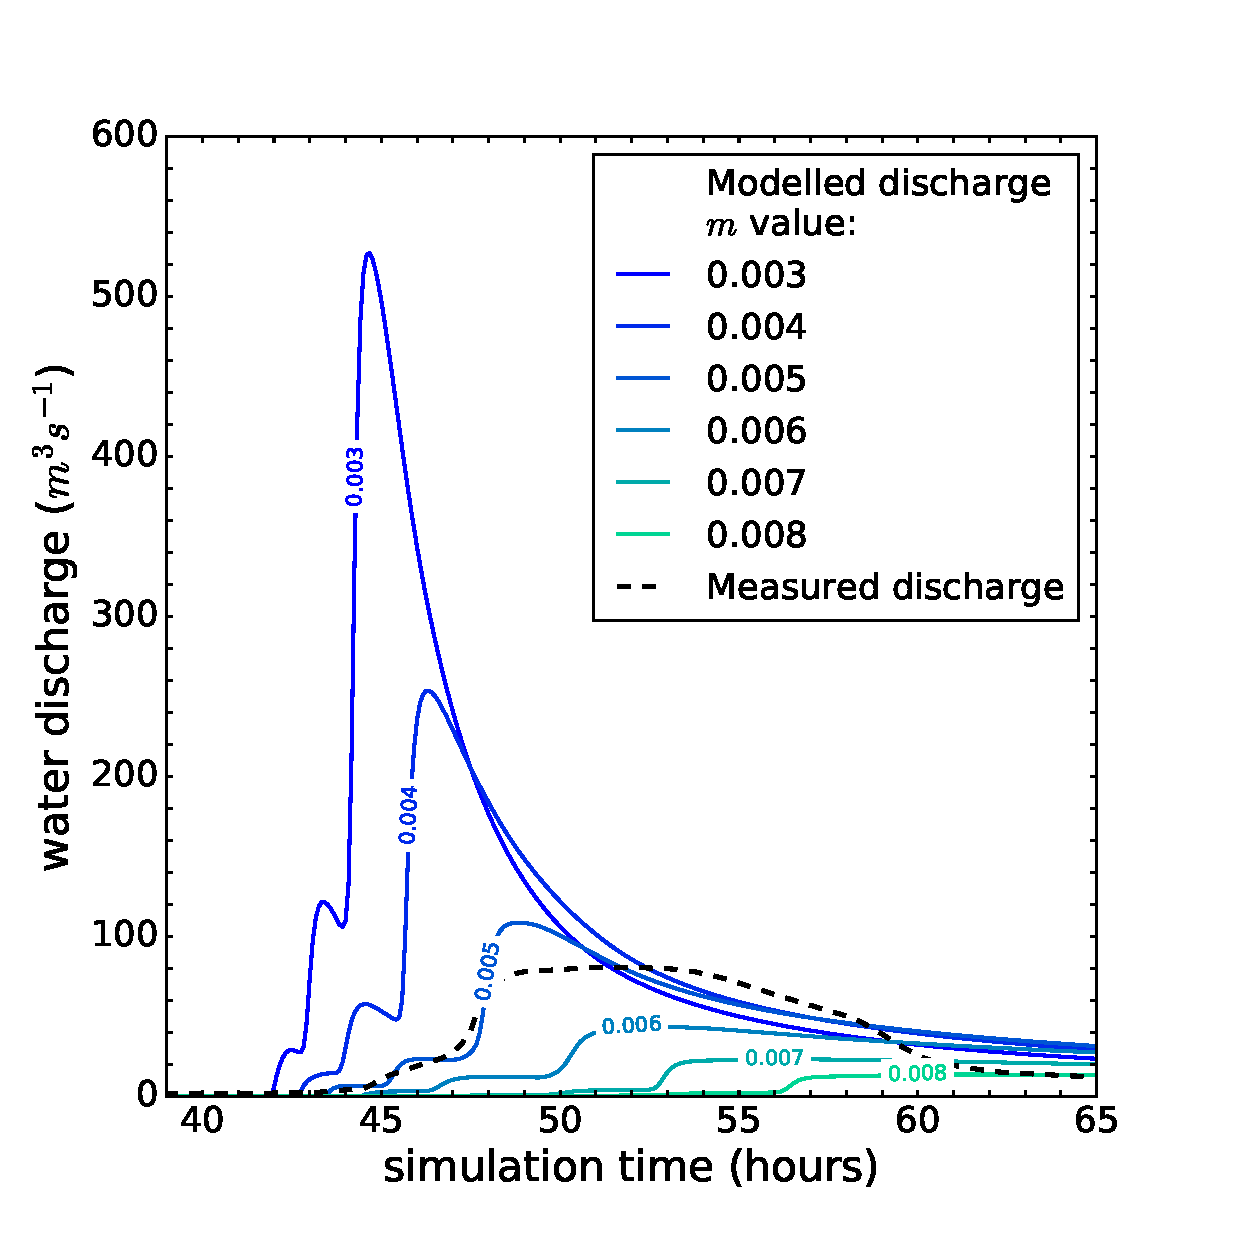
\includegraphics[width=11cm]{chp_flood_figs_scripts/fig_ryedale_hydro_m_sens_lumped.eps}
\caption{Hydrograph sensitivity to the \(m\) parameter under \textbf{uniform} rainfall inputs. Discharge over time at the Ryedale catchment outlet for varying values of the \(m\) parameter. The measured discharge at the catchment gauging station is overlaid in dashed line. The results from the simulations with \(m\) \textgreater \ 0.008 are omitted for clarity due to the low discharges they produced.}
\label{fig_topmodel_m_ryedale_lumped}
\end{figure}

\begin{figure}[!h]
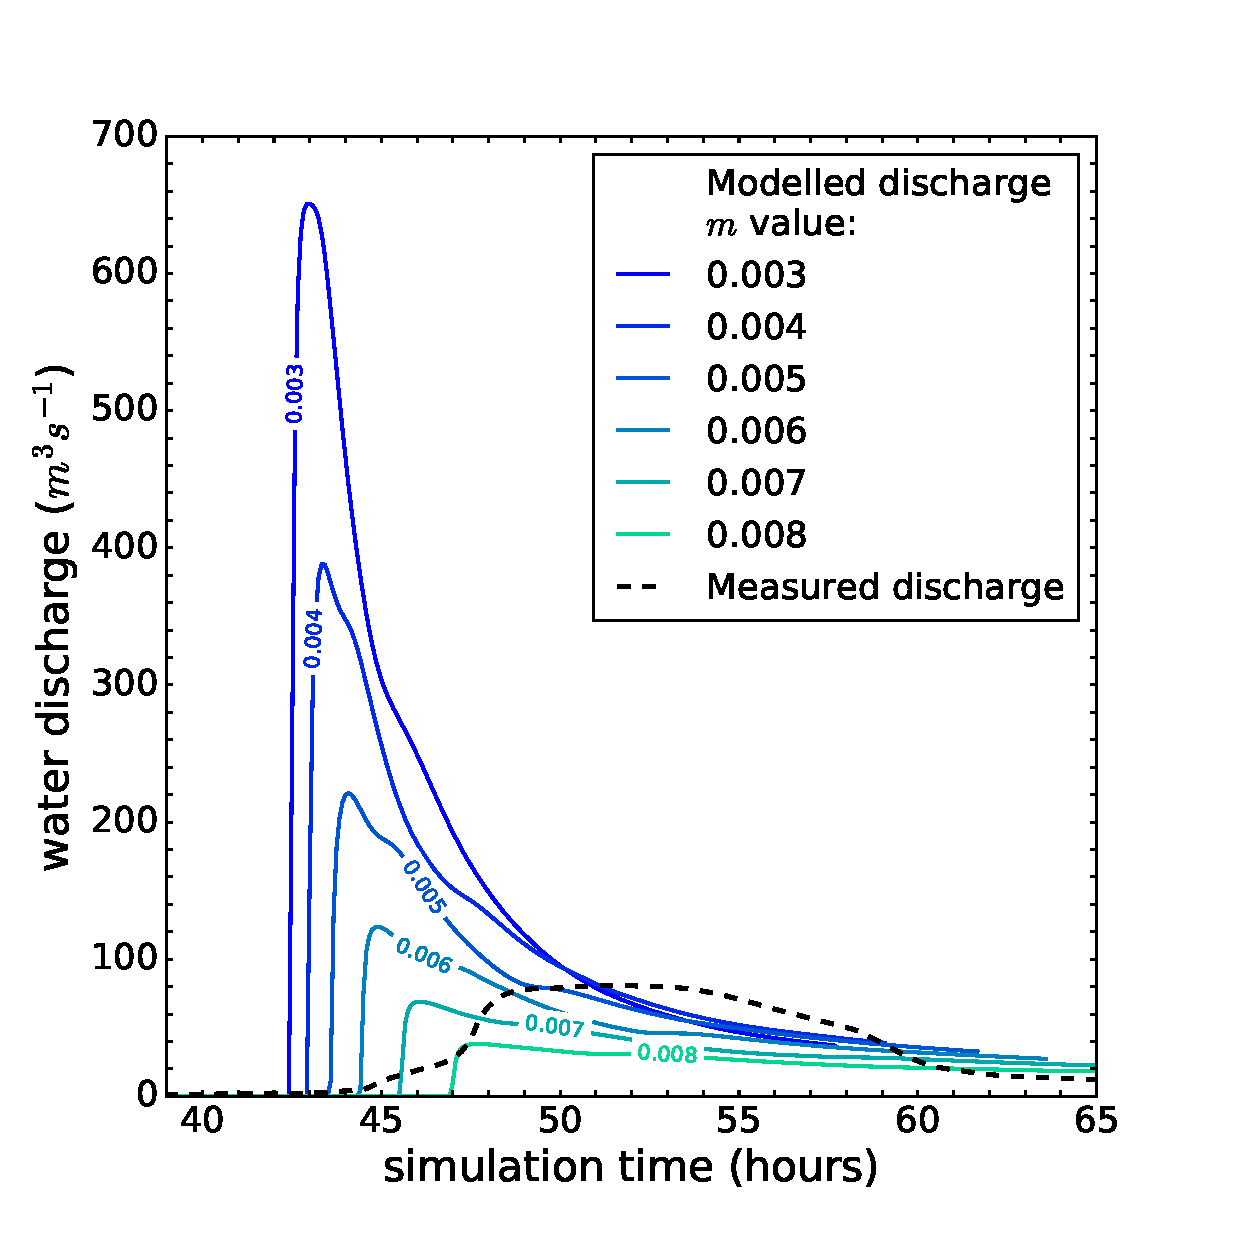
\includegraphics[width=11cm]{chp_flood_figs_scripts/fig_ryedale_hydro_m_sens_gridded.eps}
\caption{Hydrograph sensitivity to the \(m\) parameter under \textbf{gridded} rainfall inputs. Discharge over simulation time at the Ryedale catchment outlet for varying values of the \(m\) parameter. The measured discharge at the catchment gauging station is overlaid in dashed line. The results from the simulations with \(m\) \textgreater \ 0.008 are omitted for clarity due to the low discharges they produced.}
\label{fig_topmodel_m_ryedale_gridded}
\end{figure}

\subsection{Catchment hydrographs}
\label{sec_hydrographs_flood}
% AMMENDMENTS:
%Plot hyetograph (rainfall) oerlay on the hydrographs.
%For Ryedale, plot the measured observation as well from gauge. -done

%Comparisons with the actual hydrographs from the gauged basins?
\subsubsection{General observations}
At the catchment scale, hydrological response was sensitive to both the rainfall resolution and the choice of erosional model. For both catchments, higher resolution rainfall input data resulted in a greater maximum river discharge. In the Ryedale experiments, simulations using the gridded (spatially variable) rainfall input experienced a flashier hydrological response, reaching peak discharge several hours before the uniform rainfall input cases. This large difference in timing was not observed in any of the Boscastle simulations, with all simulations reaching peak discharge within 10 minutes of each other. Peak discharges and the timings of peak flow for each simulation are tabulated in Table \ref{table_discharges}.

The choice of erosion model also influenced the hydrological response. When catchment erosion was modelled using a transport-limited (\texttt{TLIM}) case, peak discharges were higher in all cases, but the timing of hydrograph peaks remained similar for each case. The difference in peak discharges was minimal when comparing the detachment-limited (\texttt{DLIM}) cases to the hydrology-only simulations.

\subsubsection{Boscastle}
The timing of peak discharge in the Boscastle catchment was similar for both the gridded and uniform rainfall simulations (Figure \ref{fig_boscastle_hydrograph_ensemble}). In gridded rainfall simulations the discharge peaked 40 hours after the start of the simulation (1600 UTC) and for the uniform rainfall input simulations at 40 hours 10 minutes into the simulation (1610 UTC). The choice of erosional parameterisation did not appear to affect the timing of the peak discharge. However, it did result in small changes in the discharge rate at peak flow, of up to 14\% difference in the uniform rainfall simulations, and 6\% increase in the gridded rainfall simulations. The primary control on the amount of discharge at peak flow appeared to be the type of rainfall inputs into the model, with the gridded simulations predicting peak discharges up to 28\% higher than their uniform counterparts. 

Comparison with measured discharge is not possible in the Boscastle case, as the basin is ungauged. However, a number of methods exist for predicting runoff and river flow in ungauged river basins \citep{sivapalan2003prediction,bloschl2013runoff}, and two estimations of discharge are presented here for comparison with the predictions from the HAIL-CAESAR model. Both estimations were derived in the \citet{wallingford2005flooding} report and the hydrographs are overlaid on the model outputs from this study in Figure \ref{fig_boscastle_hydrograph_ensemble}. The HR Wallingford report produced a simple hydrograph derived from eyewitness reports and water level marks, estimating a peak discharge of 180 m\(^3\)s\(^{-1}\) at 1600 UTC, the same as the timing of peak flow in the HAIL-CAESAR simulations. A second estimation of the hydrograph during the Boscastle event was made in the report using a one-dimensional hydraulic model, InfoWorks RS, which also predicted a peak flow of approximately 178 m\(^3\)s\(^{-1}\), but at the later time of 1700 UTC. The InfoWorks RS model uses a fixed representation of the river bed; in other words, it does not permit the topographic surface to change during the course of the model simulation. 

The estimated flow from observations and the 1D hydraulic model was higher than any of the model predictions made in this study -- a difference of 30--80 m\(^3\)s\(^{-1}\) was noted between the HAIL-CAESAR simulations and the two estimations from the HR Wallingford report. The rising and falling limbs of the hydrograph were also much shallower than the HAIL-CAESAR model predictions, which suggest a much more rapid rise and fall in water levels during the storm. 

\subsubsection{Ryedale}

The hydrological response of the Ryedale catchment was more sensitive to the choice of rainfall input type, with marked differences in the timing and magnitude of the peak discharge between the uniform and gridded rainfall sets of simulations (Table \ref{table_discharges}, Figure \ref{fig_ryedale_hydrograph_ensemble}). There is up to 83\% increase in discharge in the gridded rainfall simulations when compared to the corresponding uniform rainfall input simulations. The hydrograph was less sensitive to the type of erosional parameterisation, with up to 40\% difference observed in the uniform rainfall cases, and upto 25\% difference in the gridded rainfall simulations. 

The River Rye is gauged at several locations, and flow data was recorded during the 2005 flood, though the accuracy of gauging station data is uncertain during particularly high flow events \citep{shaw2010hydrology}. The gauge data is measured at the River Rye Ness gauging station\footnote{Environment Agency gauging station F2505 -- British National Grid reference SE 69439 79196}. The outlet of the modelled catchment domain was set up to coincide (as near as possible) with the location of the Ness gauging station on the River Rye. The observed flow data from the gauging station is overlaid in Figure \ref{fig_ryedale_hydrograph_ensemble}. The gauging station data most closely matches the hydrographs produced by the uniform rainfall inputs, though it is lower than all of the simulated hydrograph, peaking at approximately 81 m\(^3\)s\(^{-1}\). A further value of peak discharge during the Ryedale flood was reported by \citet{wass2008investigation} as 105 m \(^3\)s\(^{-1}\), derived from 1D flow modelling -- the timing of this estimated peak flow was not available due to the type of model used. The value of peak discharge reported by \citet{wass2008investigation} is similar to that of the Environment Agency gauge data and the peak flows predicted by the uniform rainfall input simulations in this study. 

The difference in timing of peak flow between the set of gridded rainfall input simulations and the uniform rainfall simulations is large; the gridded rainfall simulations predict the timing of peak flow being almost four hours earlier than the simulations using a uniform rainfall input. Observations reported in \citet{wass2008investigation} and the Environment Agency gauge support the predictions made by the uniform rainfall simulations in this case. However, this perhaps to be expected due to the fact the the TOPMODEL \(m\) value for Ryedale was calibrated using the uniform rainfall input data. The same value of \(m\) was then used with the gridded rainfall data (to ensure uniformity across  simulations) though it is likely to be mis-calibrated in this case. 

% Please add the following required packages to your document preamble:
% \usepackage{graphicx}
\begin{table}[!htbp]
\centering
\caption{Peak water discharges and corresponding times at peak flow for each of the simulation cases. Discharge is calculated at the outlet of the catchment model domain. Time is given in UTC on the day of the storm.}
\label{table_discharges}

\begin{tabular}{lcc}
\textbf{Simulation name} & \begin{tabular}[c]{@{}l@{}}\textbf{Peak discharge}\\ (m$^3$s$^{-1}$)\end{tabular} & \begin{tabular}[c]{@{}l@{}}\textbf{Time}\\ (UTC on storm day)\end{tabular} \\
\hline 
\multicolumn{3}{l}{Boscastle: 2004-08-16} \\
\hline
\texttt{GRIDDED\_HYDRO} & 151 & 1600 \\
\texttt{GRIDDED\_TLIM} & 148 & 1600 \\
\texttt{GRIDDED\_DLIM} & 143 & 1600 \\
\texttt{UNIFORM\_HYDRO} & 108 & 1610 \\
\texttt{UNIFORM\_TLIM} & 122 & 1610 \\
\texttt{UNIFORM\_DLIM} & 107 & 1610 \\
\hline
\multicolumn{3}{l}{Ryedale: 2005-06-19} \\
\hline
\texttt{GRIDDED\_HYDRO} & 221 & 2005 \\
\texttt{GRIDDED\_TLIM} & 277 & 1950 \\
\texttt{GRIDDED\_DLIM} & 232 & 2000 \\
\texttt{UNIFORM\_HYDRO} & 108 & 0050$^\dagger$ \\
\texttt{UNIFORM\_TLIM} & 151 & 2340 \\
\texttt{UNIFORM\_DLIM} & 114 & 0025$^\dagger$\\
\hline
\vspace{1em}
{\footnotesize $\dagger$ -- Time the following day}. & & \\

\end{tabular}%
\end{table}

% ENSEMBLE HYDROGRAPHS
\begin{figure}[!htbp]
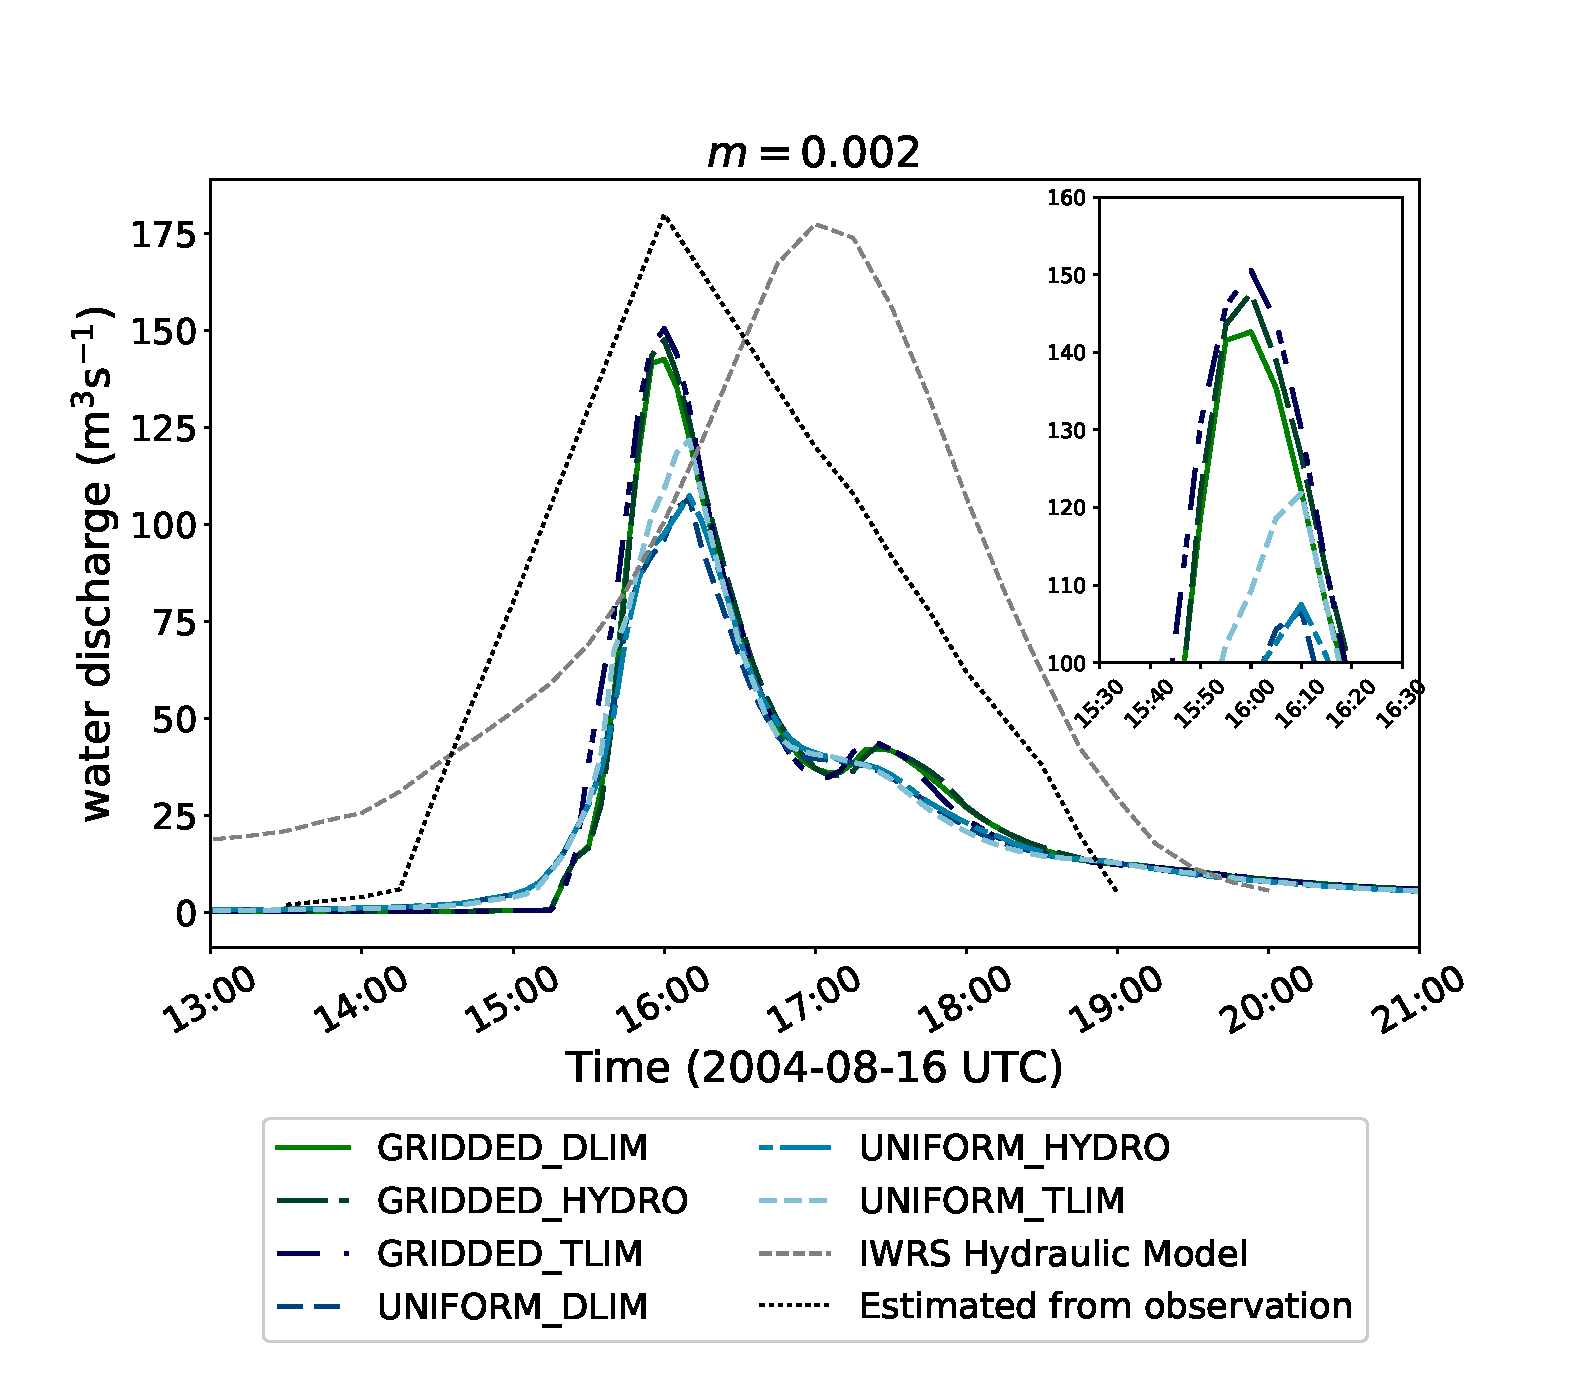
\includegraphics[width=14cm]{chp_flood_figs_scripts/fig_hydrographs_boscastle_new.eps}
\caption{Boscastle hydrographs (discharge over time at catchment outlet) for each simulation of the 2004 Boscastle event listed in Table \ref{table_ensemble_experiments}. Inset shows detail of main flood peaks around hour 40 of the simulation.}
\label{fig_boscastle_hydrograph_ensemble}
\end{figure}

\begin{figure}[!htbp]
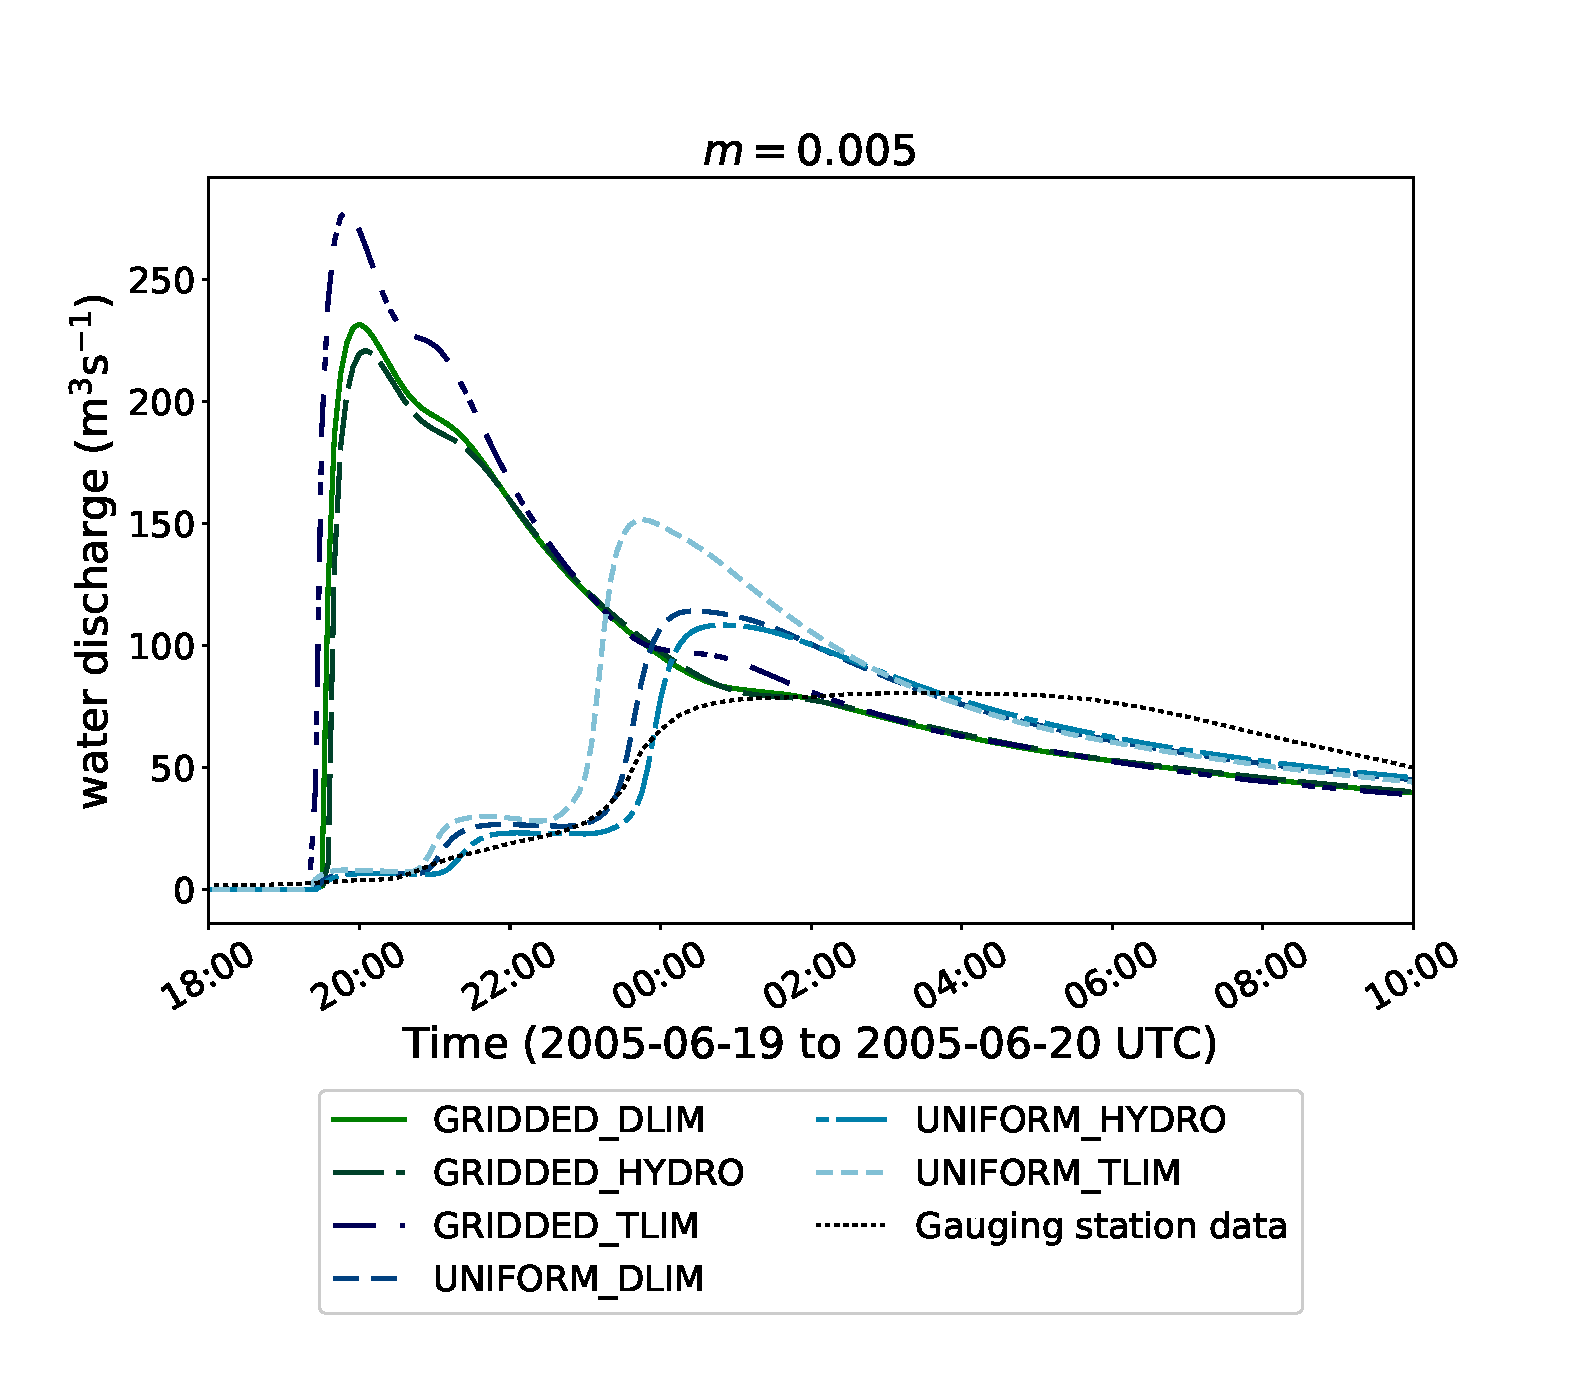
\includegraphics[width=14cm]{chp_flood_figs_scripts/fig_hydrographs_ryedale_new.eps}
\caption{Ryedale hydrographs (discharge over time at catchment outlet) for each simulation of the 2005 Ryedale event listed in Table \ref{table_ensemble_experiments}.}
\label{fig_ryedale_hydrograph_ensemble}
\end{figure}

\subsection{Flood inundation and river levels}
A series of flood inundation metrics are shown in Figures \ref{fig_inundation_area_ensemble}, \ref{fig_floodplain_depth_ensemble}, and \ref{fig_channel_depth_ensemble}, showing respectively:

\begin{enumerate}
\item Total area inundated by water
\item Mean water depth in the floodplain
\item Mean water depth in the main channel
\end{enumerate}

The floodplain area is defined for the purpose of this analysis using the \citet{clubbinpress} floodplain delineation algorithm, a method which searches for statistically significant variation in terrain relief to identify and delineate floodplains in a catchment. The `main channel' is herein defined as the mainstem channel with the highest stream order number \citep{strahler1957quantitative}, removing any tributary channels in the headwaters. The mainstem channel is delineated using a simple channel network identification algorithm based on a contributing drainage area threshold \citep{ocallaghan1984extraction,tarboton1991extraction}. The inundation metrics were derived from water depth output files created every two hours of simulated time during the model runs. As such, the absolute peak flood inundation may lie between two of the output file timesteps, but sufficient detail in spatial extents and dynamics of  the floodwaters are still captured in the analysis and the resulting figures. 

Generally, there is a tendency for the simulations with gridded rainfall input  running in hydrology-only mode (\texttt{GRIDDED\_HYDRO}) to predict the greatest extents of areal flood extent as well as floodwater depth across the floodplain and main river channel, behaviour observed in both case studies. Most simulations running in hydrology-only mode and uniform rainfall input (\texttt{UNIFORM\_HYDRO}) also predict greater flood inundation extents and peak water levels, but this tendency is less prevalent in the Ryedale simulations. In fact, the Ryedale simulations appear to be marginally more sensitive to the type of rainfall input, with both the \texttt{GRIDDED} simulations producing slightly higher peak inundation levels, regardless of whether erosion parameterisation is switched on in the model.

The starkest contrast observed was in the mean channel water depth of the Boscastle set of simulations; the difference in peak mean water depth was approximately 1 m between the hydrology-only and erosion-enabled simulations. In most of the other simulations, the differences in main channel mean water depth were smaller, on the order of tens of centimetres.

\subsubsection{Total inundation area}
Inundation area is defined here as the total area of the catchment grid cells that exceed the minimum discharge threshold at a given timestep. The minimum discharge threshold for all simulations was set as 0.03 m\(^3\)s\(^{-1}\). The inundation amounts for the Boscastle and Ryedale simulations are presented in Figure \ref{fig_inundation_area_ensemble}. For clarity, only results from one type of the erosion-enabled simulations is presented in each case (transport-limited -- \texttt{TLIM}). The predicted inundation areas for the detachment-limited erosion simulations were similar to the hydrology-only simulations, differing only by a few percentage points.

\paragraph{Boscastle}
Both of the hydrology-only simulations in the Boscastle case predicted the greatest peak in flood inundation area, with the gridded rainfall input simulations predicting slightly higher peak inundation areas. The highest predicted flood inundation area resulted from the \texttt{GRIDDED\_HYDRO} simulation, and the lowest peak from the \texttt{UNIFORM\_TLIM} simulation. The rise and fall in the areal extent of the inundated flood area is rapid, peaking within hour 40 of the simulation  (1600 UTC) and reducing by approximately 50\% by the next output time step, two hours later at 1800 UTC. 

\paragraph{Ryedale}
In the Ryedale simulations, predicted flood inundation area was again greatest in the \texttt{GRIDDED\_HYDRO} simulation and lowest in the \texttt{UNIFORM\_TLIM} simulation. In this set of simulations, both the gridded rainfall input experiments produce higher total inundation areas at the peak of the flood.

\subsubsection{Floodplain mean water depth}

Inundation area provides a general indication of the spatial extent of flooding within a catchment, but does not reveal as much about the distribution of water depths within the catchment, particularly the floodplain where many settlements are located in the Boscastle and Ryedale cases. Average floodplain water depths area presented in Figure \ref{fig_floodplain_depth_ensemble} showing how water depths rise and fall on the floodplain over the course of each storm. The average depth is calculated for each output time step (two-hourly), by averaging the water depth in each model grid cell, limited to area delineated by the floodplain-finding algorithm \citep{clubbinpress}. 

\paragraph{Boscastle}
Floodplain average water depths follow a similar pattern to that observed in the total inundation area timeseries: a sharp rise and peak corresponding to the time of maximum river discharge (1600 UTC), followed by a rapid drop-off by the time of the next model output timestep at 1800 UTC. Average water depths in the Boscastle floodplain peaked at just over 0.4 m for the \texttt{GRIDDED\_HYDRO} simulations. Average floodplain water depths for the other simulations were approximately 0.35 m, and showed little variation from this value between the different simulation parameters. %Overall there was little difference in average floodplain water depth (5 cm) predicted for the Boscastle event. 

\paragraph{Ryedale}
Water depths on the Ryedale floodplain were fast to reach their peak, but showed a more gradual recession after the flood peak than the Boscastle simulations. The highest mean floodplain water depths were predicted by the \texttt{GRIDDED\_HYDRO} simulations at 0.16 m, though the difference between other simulations was minimal -- the lowest predicted mean depths of 0.14 m were observed in the \texttt{UNIFORM\_TLIM} simulation, a difference of only 2 cm. The timings of peak water depth were slightly different between the gridded rainfall and uniform rainfall simulations, with uniform rainfall input simulations peaking 2--3 hours after the gridded rainfall input simulations, mirroring the pattern seen the Ryedale hydrographs (Figure \ref{fig_ryedale_hydrograph_ensemble}).

\subsubsection{River channel water depth}
Water depths in the river channel are determined by reporting the water depth along the channel midpoint, determined by a channel network extraction algorithm \citep{Braun2013}. Modification of the floodplain finding algorithm was considered to extract the entire channel footprint and average over the full channel width, but limitations in the algorithm's ability to delineate the channel in the 5 m digital elevation model prevented this and so the channel midpoint was used as a representative sampling point of water depth. The channel section over which the average depth was taken was defined as the highest order channel in the catchment, i.e. the main channel stem into which all the other catchment tributaries flow.

%Any level data for Rye?
\paragraph{Boscastle}
In the Boscastle catchment, (River Valency channel), peak mean channel water depths range from 2.4 m in the \texttt{GRIDDED\_HYDRO} simulation to 1.2 m in the \texttt{GRIDDED\_TLIM} simulations. There is a noticeable difference between the channel mean water depths at peak flow in the erosion-enabled simulations, which range between 1.2--1.4 m, and the mean depths in the hydrology-only simulations, both of which exceed 2 m. Modelling of river levels carried out by \citet[][figures 6.14, 6.15 in the report]{wallingford2005flooding} using a one-dimensional hydraulic model predicted water levels in the Valency river channel ranging between 1--3 metres at the peak of the flood, within a similar range to the river channel levels predicted the HAIL-CAESAR simulations presented here. 

\paragraph{Ryedale}
In the main channel of the River Rye, peak water depths range from approximately 1.2--1.5 m, a notably smaller range in depth than the Boscastle simulations. The highest mean water depths were predicted by the \texttt{GRIDDED\_HYDRO} simulations. The other simulations predicted very similar peak mean channel water depths, around 1.3 m. The lowest mean depths were predicted by the \texttt{UNIFORM\_TLIM} simulation.  

% ENSEMBLE INUNDATION AND DEPTHS
\begin{figure}[!htbp]
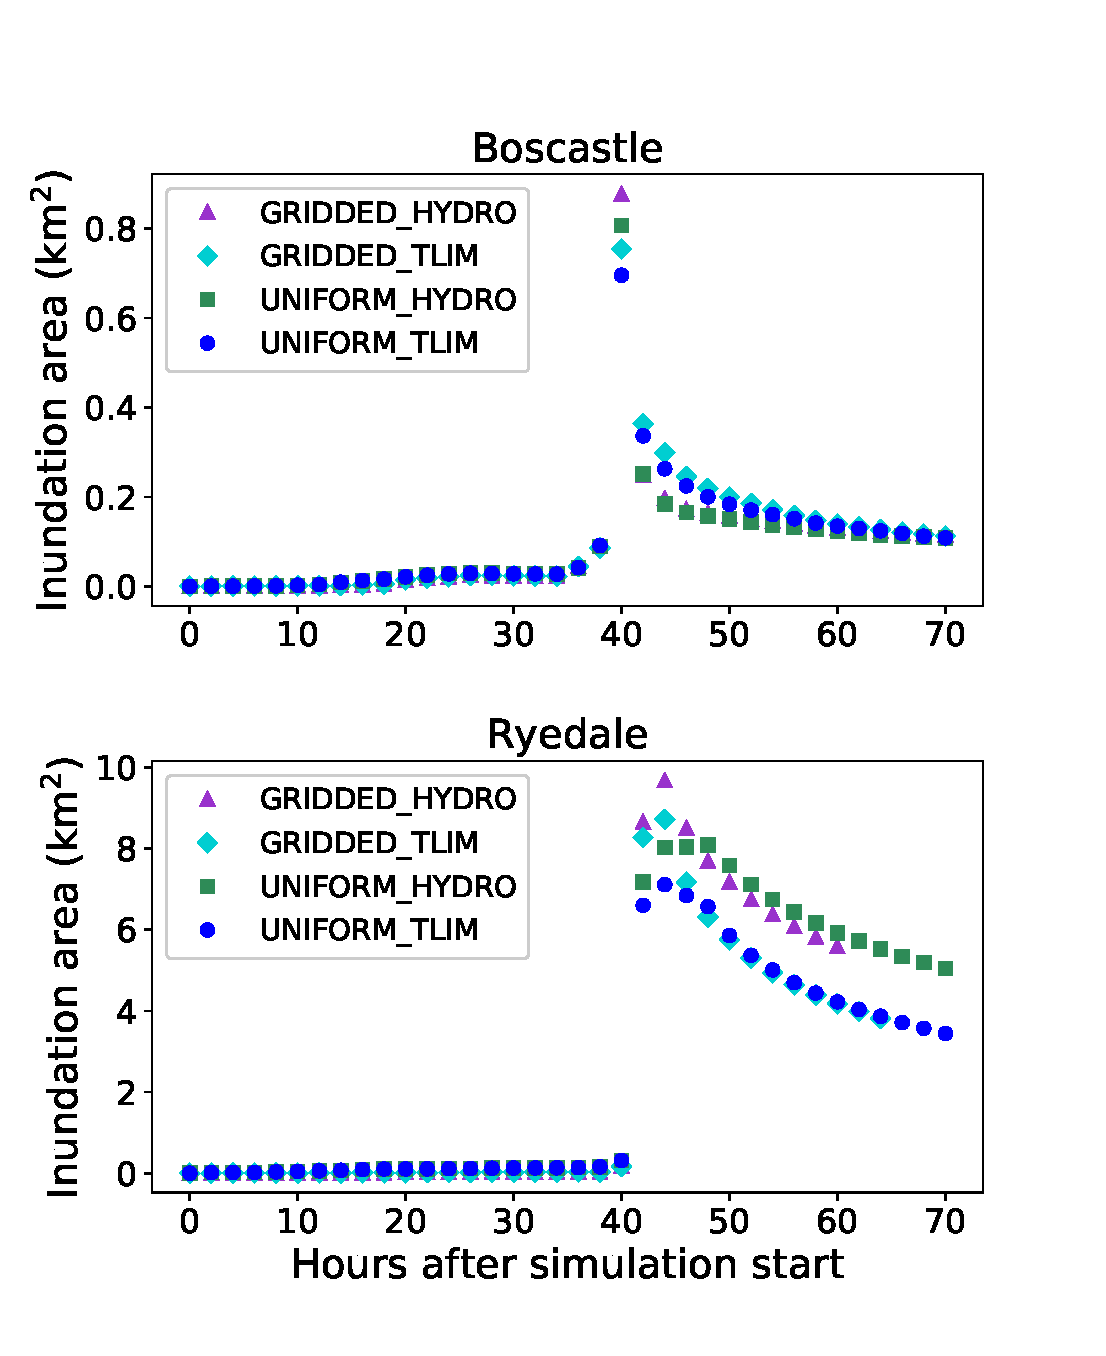
\includegraphics[width=12cm]{chp_flood_figs_scripts/inundation_area.eps}
\caption{Total inundation area (km$^2$) covered by floodwaters in the Boscastle (top) and Ryedale (bottom) catchments throughout the duration of the each storm. Inundation area is shown for each combination of flood-only, erosion-enabled, gridded rainfall input, and uniform rainfall input simulation. The erosion-enabled simulations use the transport-limited erosion law (\texttt{TLIM}). Detachment limited erosion cases were omitted for clarity.}
\label{fig_inundation_area_ensemble}
\end{figure}

\begin{figure}[!htbp]
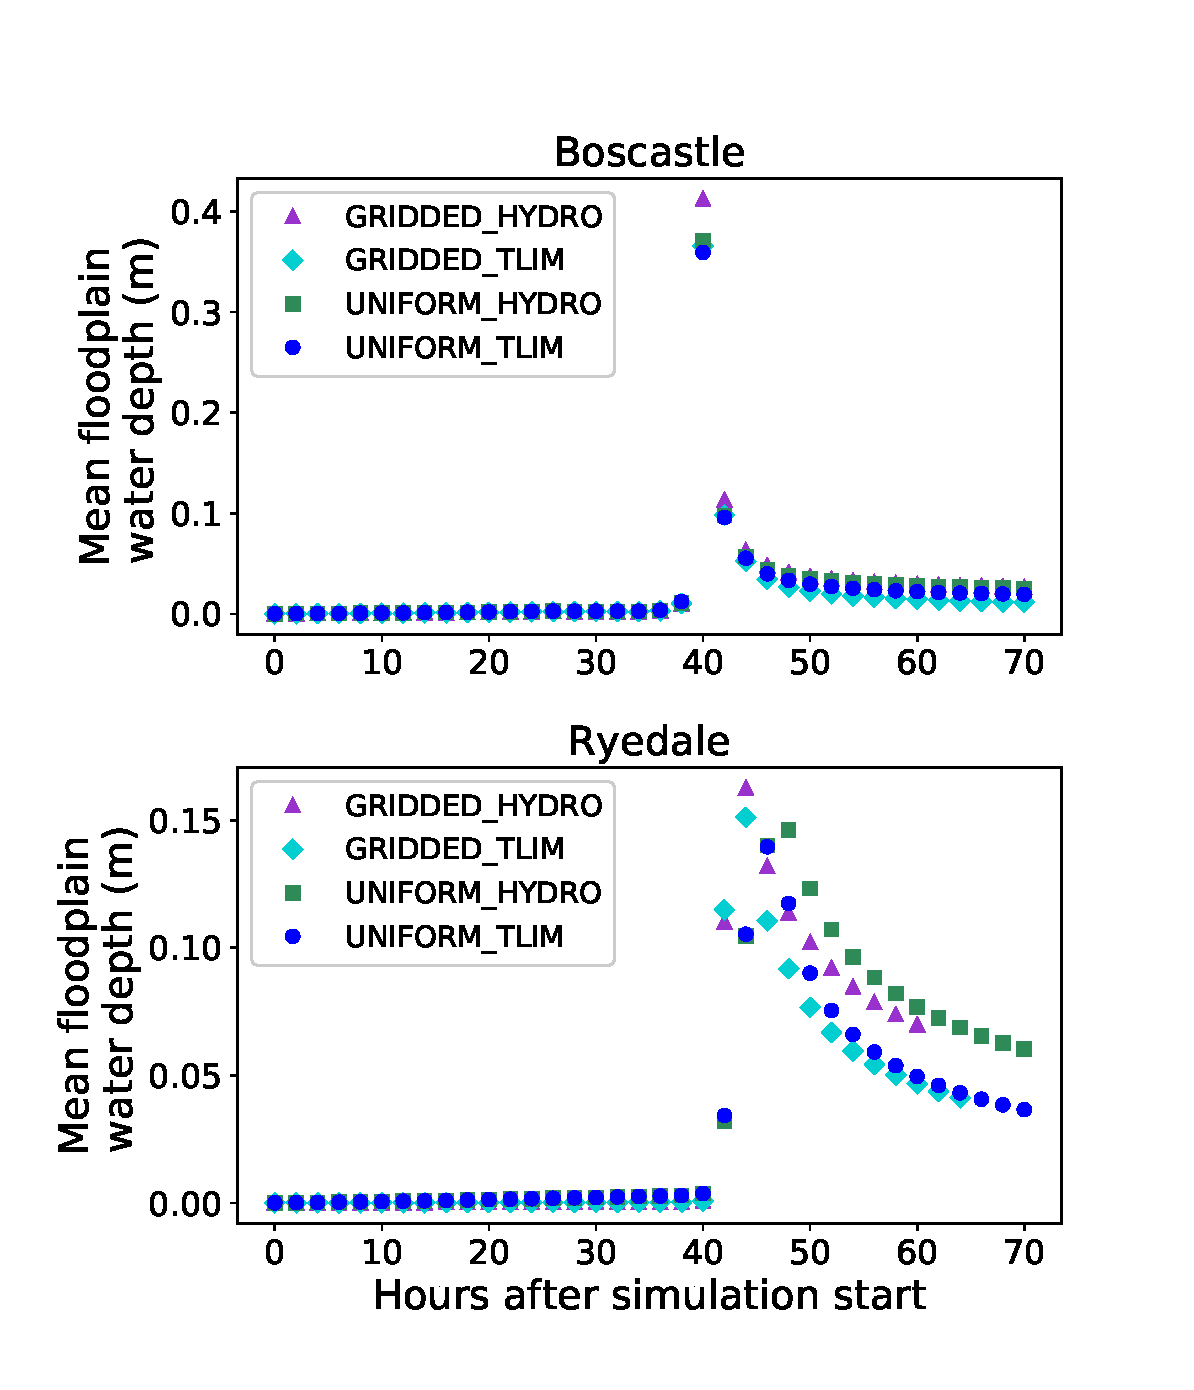
\includegraphics[width=12cm]{chp_flood_figs_scripts/floodplain_mean_depth.eps}
\caption{Mean floodplain water depth (metres) in the Boscastle (top) and Ryedale (bottom) catchments throughout the duration of the each storm. Floodplain is defined using the \citet{clubbinpress} floodplain delineation algorithm.) Water depth is shown for each combination of flood-only, erosion-enabled, gridded rainfall input, and uniform rainfall input simulation. The erosion-enabled simulations use the transport-limited erosion law (\texttt{TLIM}). Detachment limited erosion cases were omitted for clarity.}
\label{fig_floodplain_depth_ensemble}
\end{figure}

\begin{figure}[!htbp]
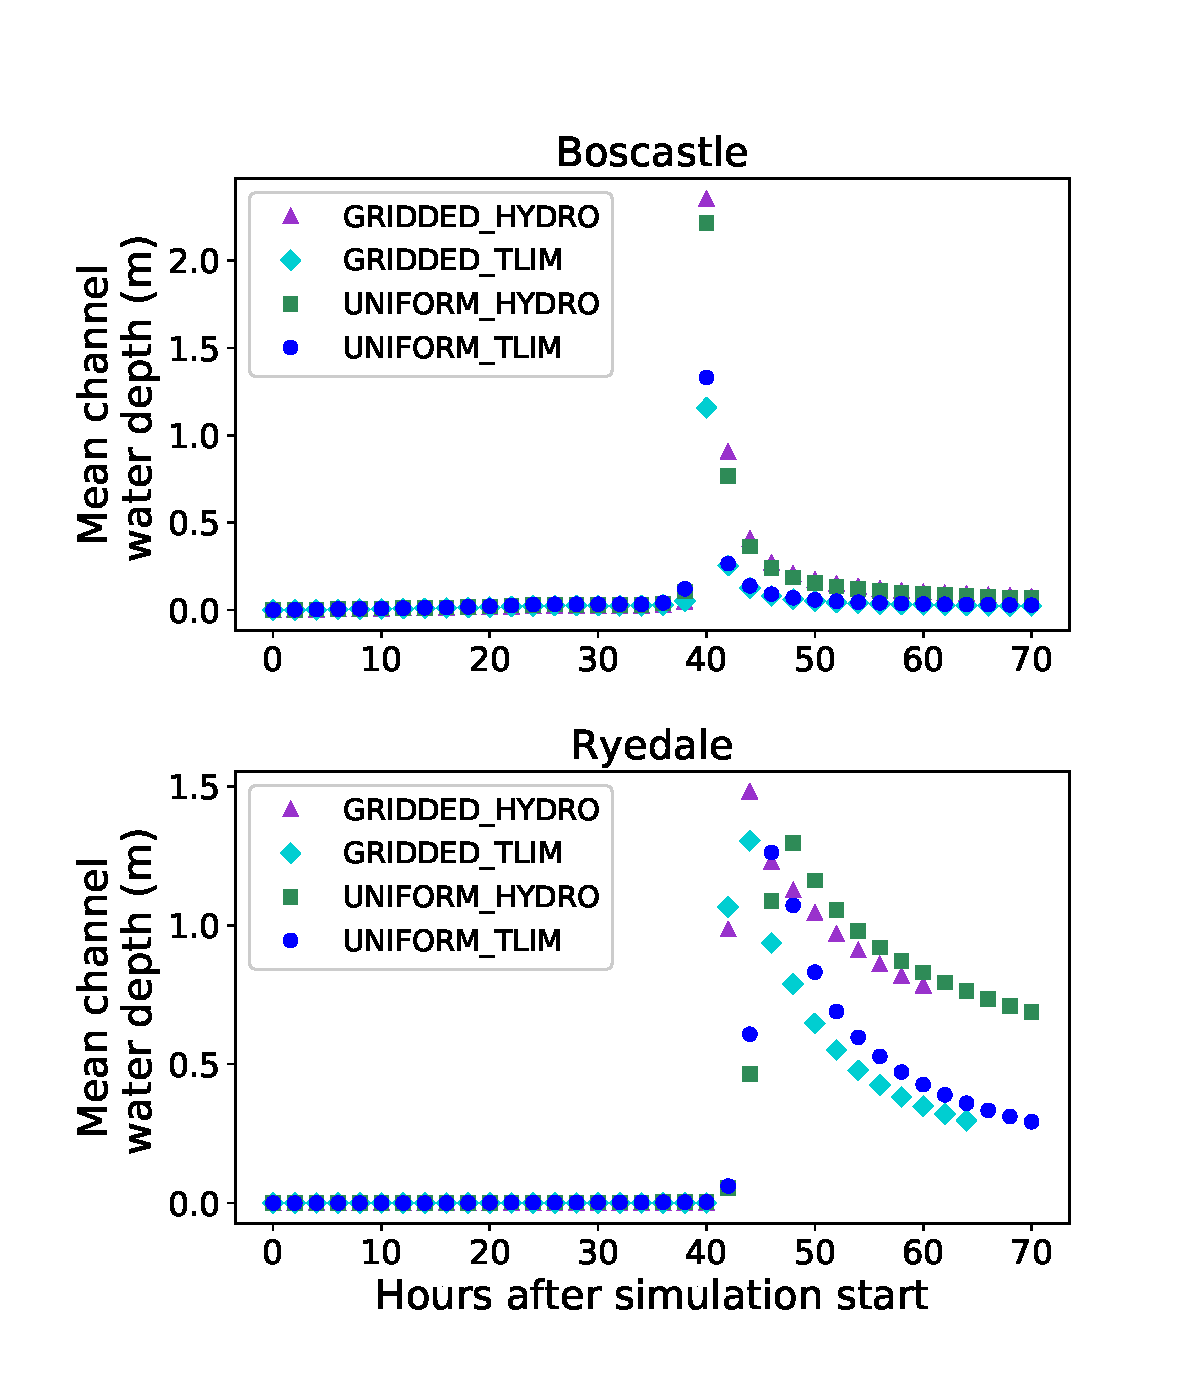
\includegraphics[width=12cm]{chp_flood_figs_scripts/channel_mean_depth.eps}
\caption{Main channel mean water depth (metres) in the Boscastle (top) and Ryedale (bottom) catchments throughout the duration of the each storm. The main channel is defined as the highest-order stream in each catchment \citep{strahler1957quantitative} and excludes all minor tributaries. Water depth is shown for each combination of flood-only, erosion-enabled, gridded rainfall input, and uniform rainfall input simulation. The erosion-enabled simulations use the transport-limited erosion law (\texttt{TLIM}). Detachment limited erosion cases were omitted for clarity.}
\label{fig_channel_depth_ensemble}
\end{figure}


\subsection{Spatial variation in flood inundation}
Thus far, the analysis of the model output has concerned catchment wide hydrological outputs and average water depths during flooding in the form of two-dimensional time series. The following section considers the spatial distribution of floodwaters across the catchments at the peak of each flood event. Comparisons between the spatial distribution of floodwaters under different model parameterisations are presented in Figures \ref{fig_boscastle_2dplan_flood_ensemble_town}, \ref{fig_boscastle_2dplan_flood_ensemble_confluence} (Boscastle), and Figures \ref{fig_ryedale_2dplan_flood_ensemble_floodplain}, \ref{fig_ryedale_2dplan_flood_ensemble_town}, \ref{fig_ryedale_2dplan_flood_ensemble_upstream} (Ryedale). An overview of the catchments and location of the main settlement in each is presented in Figure \ref{fig_boscastle_2dplan_inset_loc} and \ref{fig_ryedale_2dplan_location_insets}.

\subsubsection{Boscastle}
The Boscastle catchment simulations showed minimal variation in flood inundation extent. Simulations with gridded rainfall input did not result in substantially different predictions of floodwater inundation compared to those with uniform rainfall input. Both sets of simulations reflected the general extent of reported flood water extents \citep{wallingford2005flooding}. Simulations that allowed erosion to take place (\texttt{GRIDDED\_TLIM} and \texttt{UNIFORM\_TLIM}) showed a slight difference in the variation of floodwater depths in the floodplain area, particularly in the vicinity of Boscastle village, where Figure \ref{fig_boscastle_2dplan_flood_ensemble_town} is centred on. In hydrological-only simulations, the deepest water depths were predicted to occur in the confines of the river channel, whereas in erosion-enabled simulations, there appeared to be a `smoothing' effect of water depths between the channel and the adjacent floodplain, suggesting that the channel geometry had altered during the flood event either by infilling from sediment from upstream or collapse of the adjacent river banks -- this effect is particularly evident in Figure \ref{fig_boscastle_2dplan_flood_ensemble_confluence}. Post-event reports of the Boscastle flood noted that the river channel in the Boscastle village area had indeed been inundated with debris during the storm, which had potentially contributed to the extent of the flooding within the village. The debris blockage of the  river channel as it flowed under the road bridge in the centre of the village was also noted as a potential contributory factor to the pattern of flood inundation during the storm. Overall, the results from the Boscastle simulations indicate that although the general differences in flood extent are minimal, there are small localised variations in the distribution of flood water depths at key locations, which can be attributed to the parameterisation of erosional processes in the simulations (Figure \ref{fig_boscastle_2dplan_flood_ensemble_town} and \ref{fig_boscastle_2dplan_flood_ensemble_confluence}).

\subsubsection{Ryedale}
The Ryedale simulations showed less variation in flood extents between the gridded rainfall and uniform rainfall inputs. The flood extents were only slightly greater in the gridded rainfall input simulations, despite the much higher peak discharges predicted in these simulations (Figure \ref{fig_ryedale_hydrograph_ensemble}). The main areas where flood extents were greater were in the floodplain area south of Helmsley (Figure \ref{fig_ryedale_2dplan_flood_ensemble_floodplain}) and in certain places around the settlement of Helmsley (Figure \ref{fig_ryedale_2dplan_flood_ensemble_town}).  The variation in water depths appeared to be less sensitive in comparison to the Boscastle simulations. In the lower reaches of the catchment (Figure \ref{fig_ryedale_2dplan_flood_ensemble_town}), there appeared to be little indication that flood extents or water depths were sensitive to the erosion parameterisation, in contrast to the Boscastle simulations.

%LOCATION MAP BOS
\begin{figure}[!htbp]
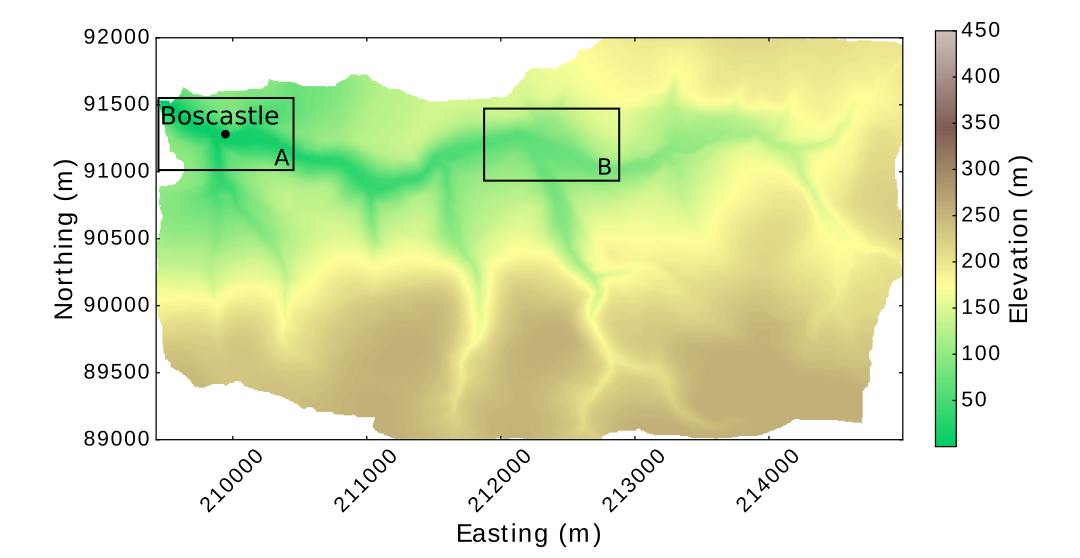
\includegraphics[width=14cm]{chp_flood_figs_scripts/fig_boscastle_catchment_insets.png}
\caption{Location map of the Boscastle catchment and Valency river valley, with the village of Boscastle shown. Location of the zoom-in images in Figures \ref{fig_boscastle_2dplan_flood_ensemble_town} (A) and \ref{fig_boscastle_2dplan_flood_ensemble_confluence} (B) shown in rectangular outlines.}
\label{fig_boscastle_2dplan_inset_loc}
\end{figure}

% Plan view flood maps BOSCASTLE
\begin{sidewaysfigure}[!htbp]
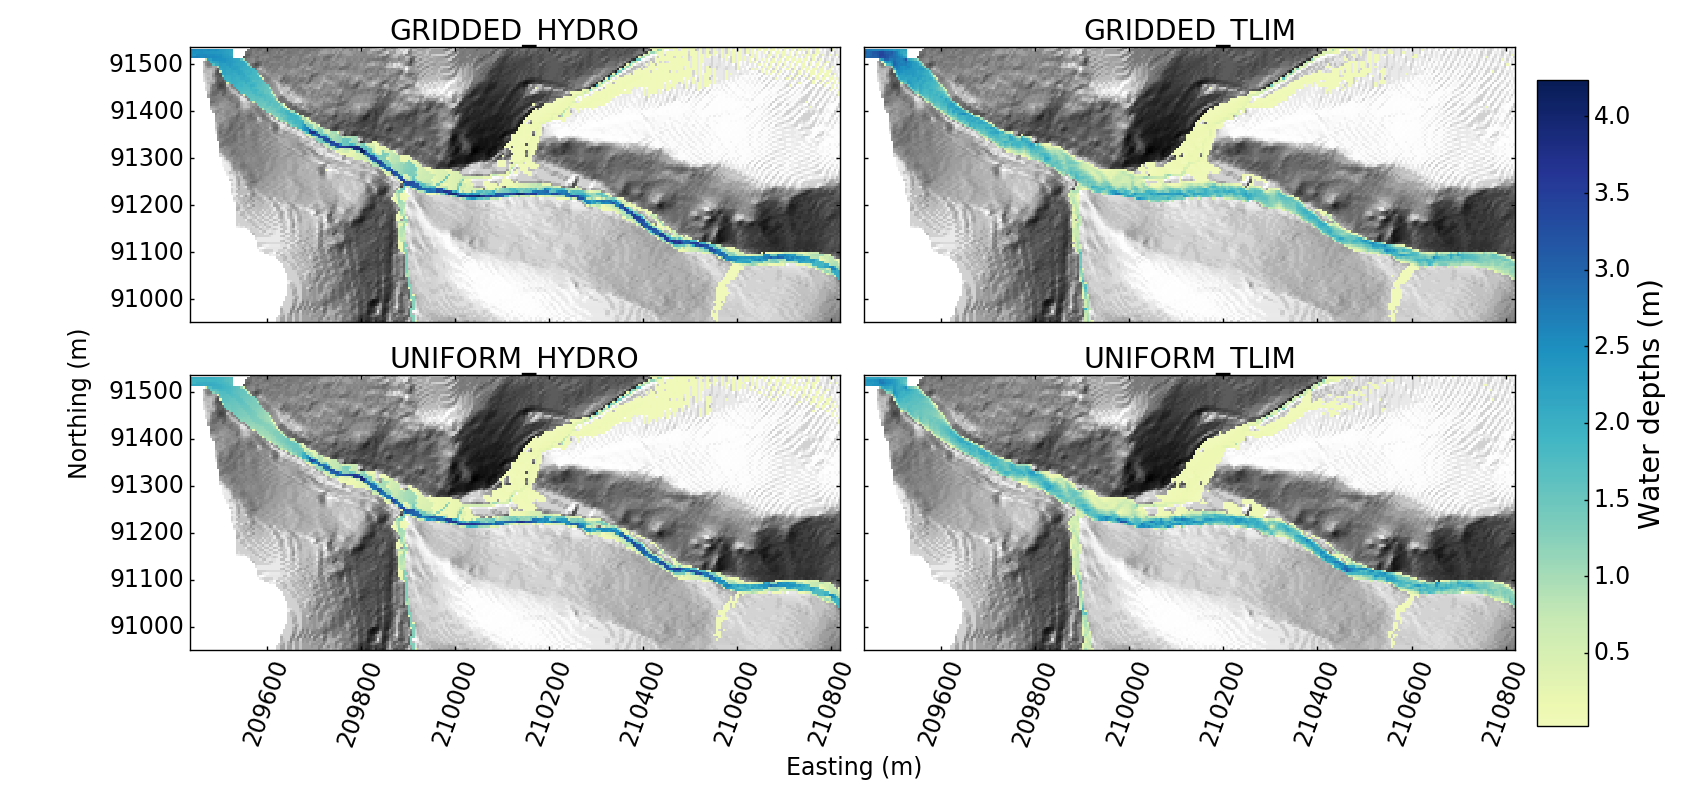
\includegraphics[width=24cm]{chp_flood_figs_scripts/fig_boscastle_flood_enseble_town.png}
\caption{Flood extents in the Boscastle catchment around the village area (location A on the overview map in Figure \ref{fig_boscastle_2dplan_inset_loc}) at the time of maximum river discharge for each simulation. }
\label{fig_boscastle_2dplan_flood_ensemble_town}
\end{sidewaysfigure}

\begin{sidewaysfigure}[!htbp]
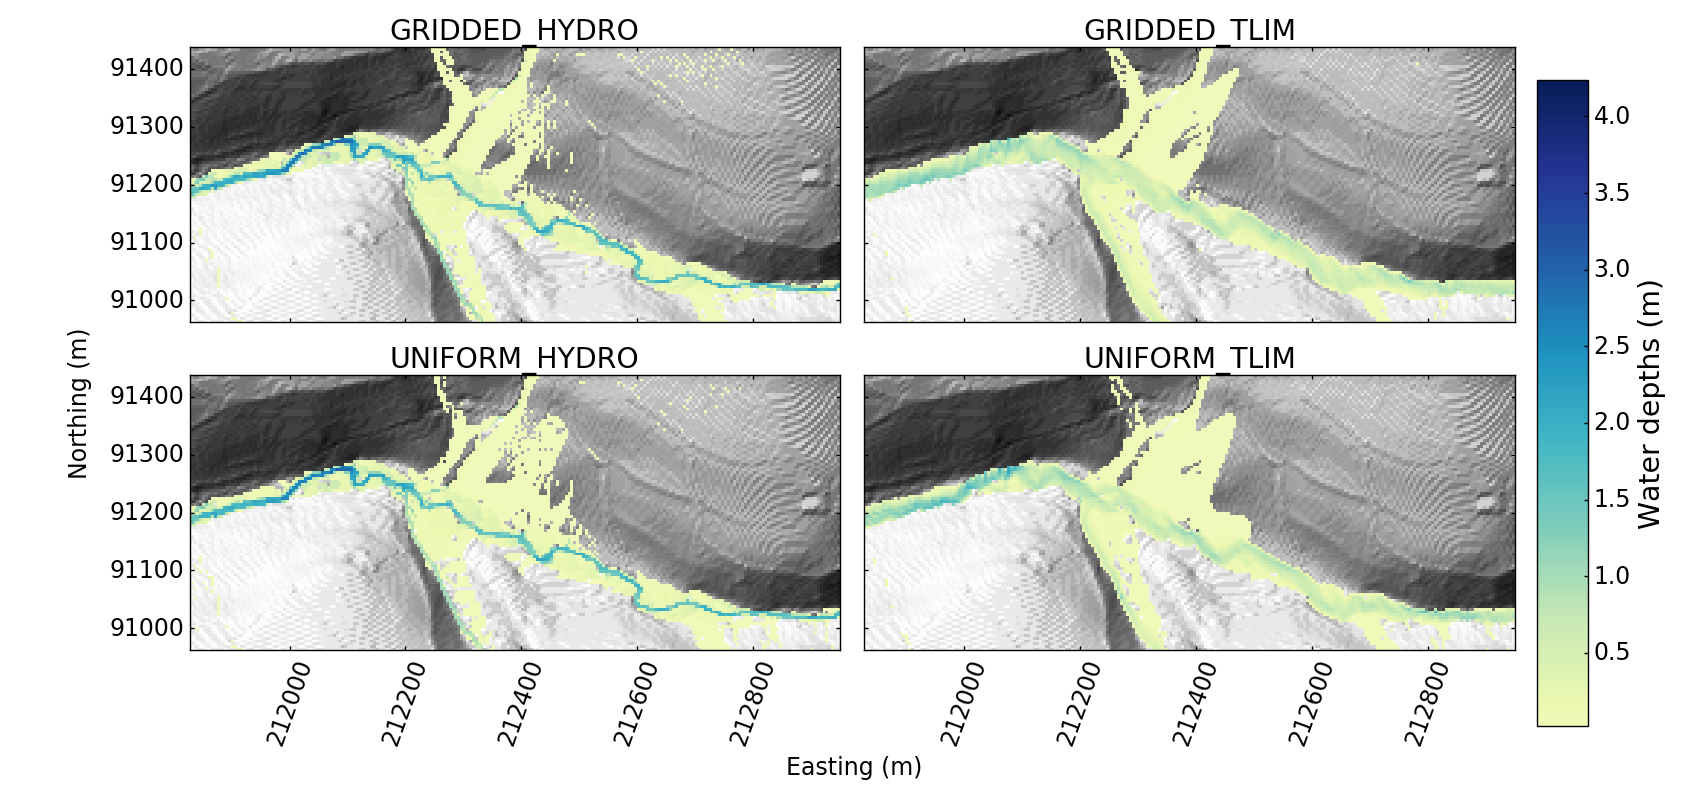
\includegraphics[width=24cm]{chp_flood_figs_scripts/fig_boscastle_flood_enseble_confluence.png}
\caption{Flood extents in the Boscastle catchment around the upstream confluence area (location B on the overview map in Figure \ref{fig_boscastle_2dplan_inset_loc}) at the time of maximum river discharge for each simulation.}
\label{fig_boscastle_2dplan_flood_ensemble_confluence}
\end{sidewaysfigure}

% Plan view flood  maps RYEDALE
\begin{figure}[!htbp]
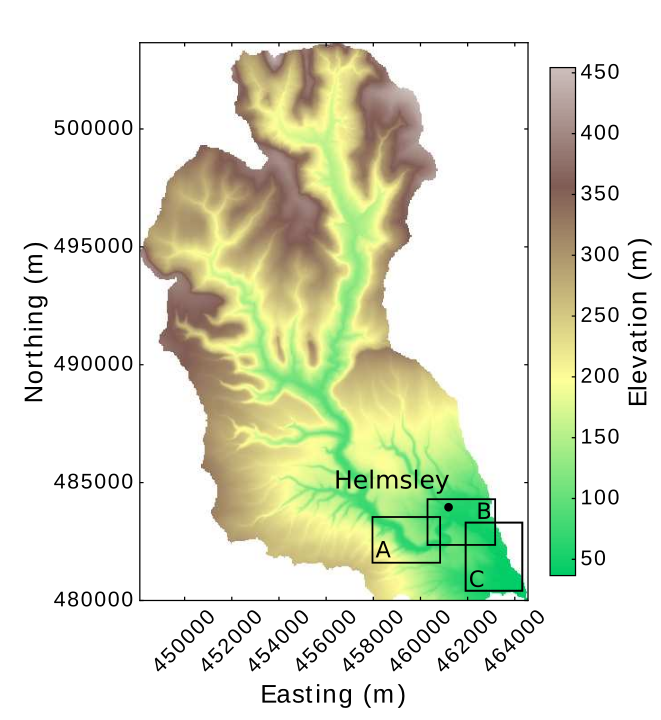
\includegraphics[width=12cm]{chp_flood_figs_scripts/fig_ryedale_catchment_location_insets.png}
\caption{Location map of the Ryedale catchment and Rye river valley, with the village of Helmsley shown. Location of the zoom-in images in Figures \ref{fig_ryedale_2dplan_flood_ensemble_floodplain} (A), \ref{fig_ryedale_2dplan_flood_ensemble_town} (B), and \ref{fig_ryedale_2dplan_flood_ensemble_upstream} (C) shown in rectangular outlines.}
\label{fig_ryedale_2dplan_location_insets}
\end{figure}

\begin{sidewaysfigure}[!htbp]
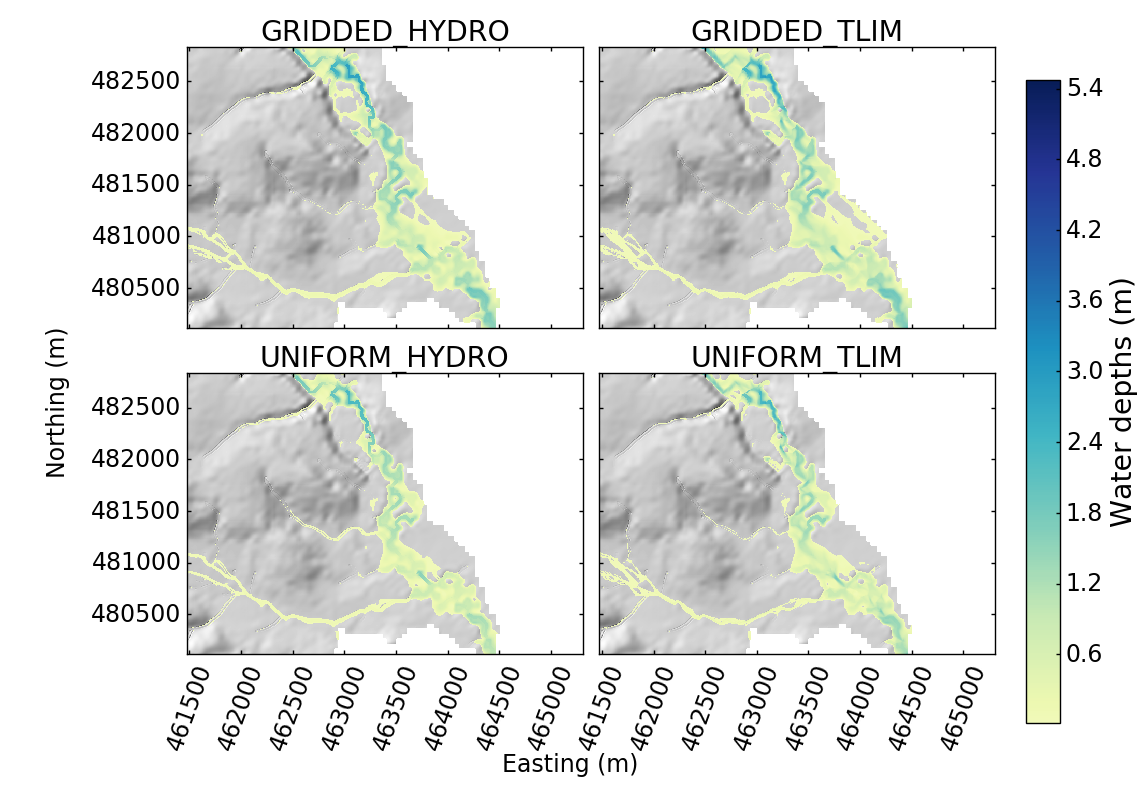
\includegraphics[width=20cm]{chp_flood_figs_scripts/fig_ryedale_flood_ensemble_floodplain.png}
\caption{Flood extents in the Ryedale catchment in the floodplain area south of Helmsley (location C on the overview map in Figure \ref{fig_ryedale_2dplan_location_insets}) at the time of maximum river discharge for each simulation.}
\label{fig_ryedale_2dplan_flood_ensemble_floodplain}
\end{sidewaysfigure}

\begin{sidewaysfigure}[!htbp]
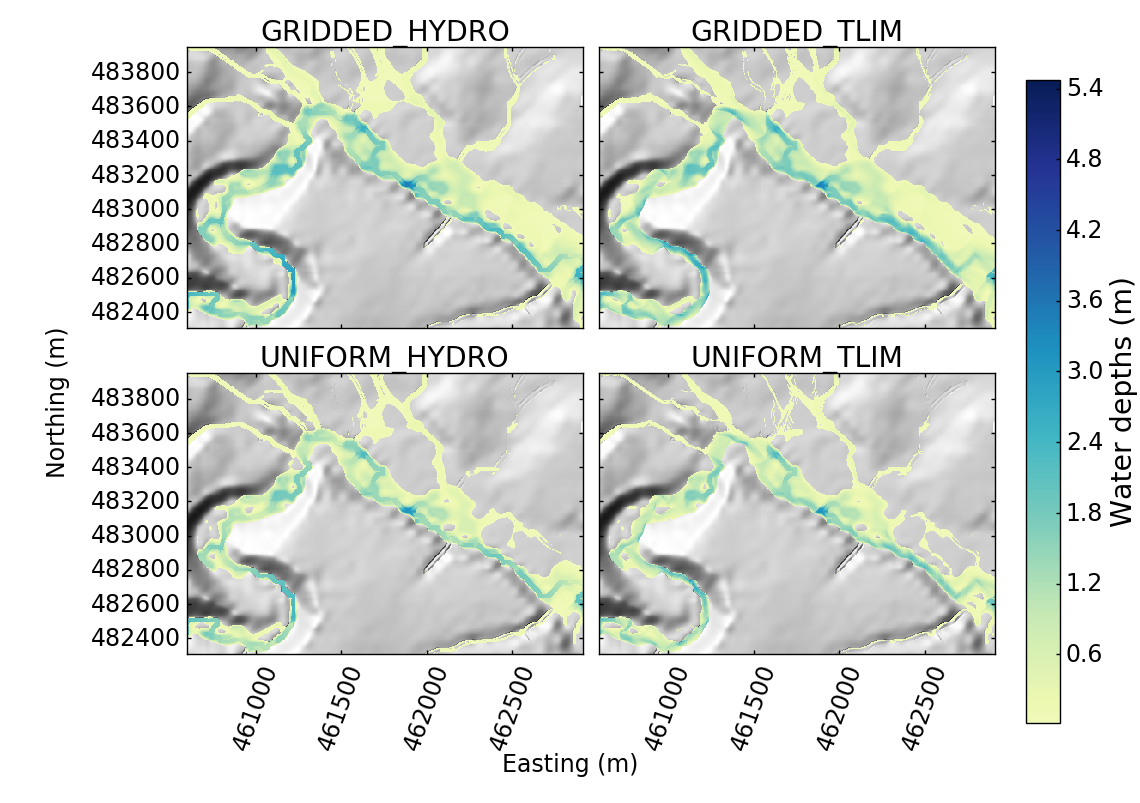
\includegraphics[width=20cm]{chp_flood_figs_scripts/fig_ryedale_flood_ensemble_helmsely.png}
\caption{Flood extents in the Ryedale catchment in the area surrounding Helmsley village (location B on the overview map in Figure \ref{fig_ryedale_2dplan_location_insets}) at the time of maximum river discharge for each simulation.}
\label{fig_ryedale_2dplan_flood_ensemble_town}
\end{sidewaysfigure}

\begin{sidewaysfigure}[!htbp]
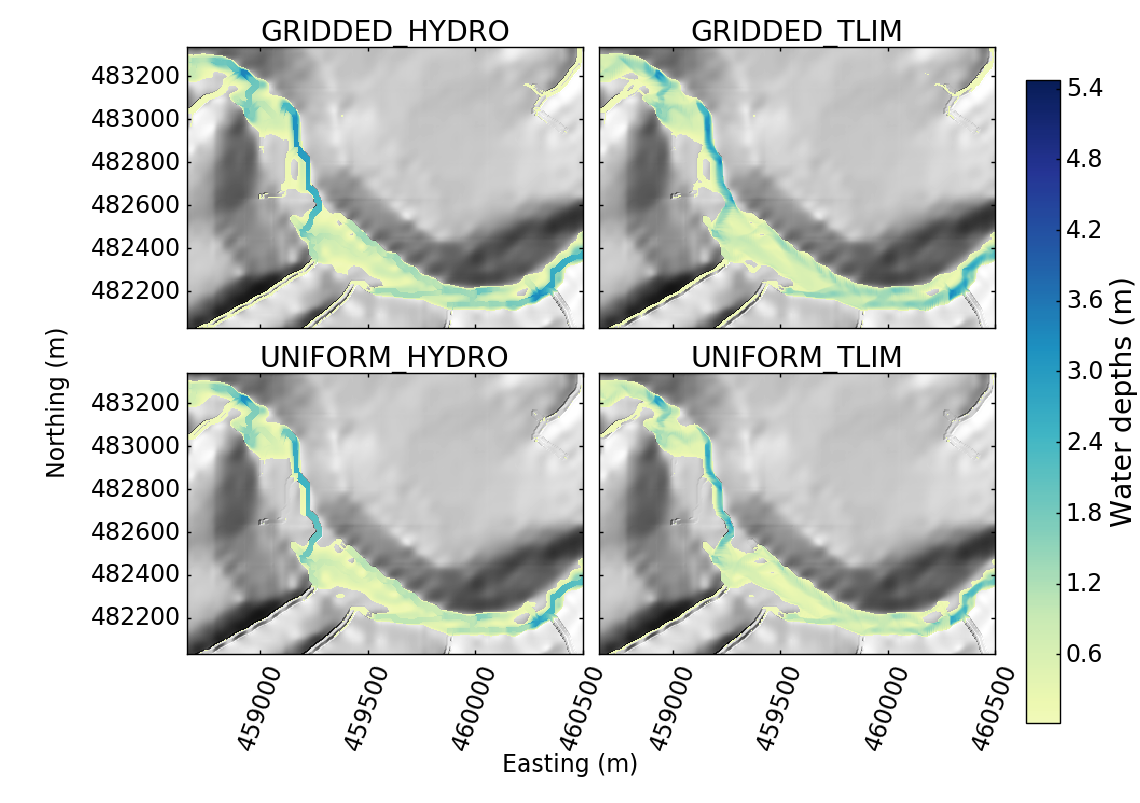
\includegraphics[width=20cm]{chp_flood_figs_scripts/fig_ryedale_flood_ensemble_upstream.png}
\caption{Flood extents in the Ryedale catchment in the gorge area west of Helmsley village (location A on the overview map in Figure \ref{fig_ryedale_2dplan_location_insets}) at the time of maximum river discharge for each simulation.}
\label{fig_ryedale_2dplan_flood_ensemble_upstream}
\end{sidewaysfigure}

\section{Discussion}

The aim of this chapter was to explore how modelled flood hydrology and flood inundation extents are sensitive to two external factors: the spatial resolution of precipitation inputs and the parameterisation of erosional processes. An ensemble simulation approach was taken using a cellular automaton landscape evolution and hydrological model to simulate two historic case studies of flash flooding events in the UK, varying the parameterisations of erosion and rainfall spatial resolution in each simulation. The results paint a complex picture of the competing controls of 1) spatial resolution of rainfall input and 2) erosional processes representation within the catchment.

\subsection{Rainfall spatial resolution}
In comparison to erosional parameterisation, the spatial resolution of rainfall input to the catchment exhibits a first-order control on its hydrological response during the flash flood event in both of the case studies presented here. Hydrographs from the Ryedale simulations were noticeably different in the prediction of the magnitude and timing of peak discharges, although in the smaller Boscastle catchment the differences in hydrological response were smaller, both in terms of the difference in timing of the peak flow and the peak water discharge rate. There are size differences between the two catchments studied -- the Ryedale catchment (270 km\(^2\)) is an order of magnitude larger in area than Boscastle (18 km\(^2\)) -- and such differences in catchment size have previously (although not conclusively) been argued to control the sensitivity of catchments to spatial variability in rainfall inputs \citep{krajewski1991monte,nicotina2008impact}. Although it has been argued that smaller catchments up to around 3500 km\(^2\) are largely insensitive to spatial variability in rainfall input due to a alack of heterogeneity in rainfall structures relative to the size of the catchment  \citep{nicotina2008impact}, the results in this study suggest catchments around 250 km\(^2\) in size are sensitive to the spatial variability in rainfall inputs during intense rainfall events. For each simulation using gridded rainfall input, the cell width of the rainfall grid is 1 km. The relative amount of increase in rainfall detail between uniform and gridded simulations is potentially much greater in the larger Ryedale catchment than the Boscastle catchment. By using a 1 km gridded rainfall product as input data, the Ryedale simulation potentially captures 15 times more rainfall heterogeneity compared to the respective Boscastle simulation, by virtue of it simply being a much larger catchment with a greater number of rainfall input cells. 

The results from this study support the general consensus that there is some degree of sensitivity in catchment hydrology to rainfall spatial inputs, but in contrast to other studies, this sensitivity may be observed in much smaller catchments than previously thought. Furthermore, the flood inundation model used in this study appears to be more sensitive to spatial heterogeneity in rainfall inputs than it is to erosional parameterisation within the model, which may extend to hydrological modelling and flood forecasting in general. Further studies with different numerical models and different rainfall events would be needed to confirm this. 

The findings here potentially offer some explanation to other other studies that have shown over longer timescales, hydrological outputs from catchments simulated with spatially variable rainfall input data can see significant increases in mean annual discharge \citep{coulthard2016sensitivity}. If individual events can show notable differences in hydrological outputs, over time this will lead to larger differences in mean annual discharges. The general idea of catchment-size sensitivity to rainfall inputs is not challenged, but there is still a lack of consensus at what spatial scale this becomes a dominating factor. These findings suggest that catchments smaller than previously thought are also sensitive to rainfall spatial heterogeneity.

A secondary aim of this study was to investigate whether spatially detailed rainfall data leads to more accurate hydrological predictions, not merely \textit{different} predictions. Where available, measurements of the timing, magnitude, and spatial distribution of flood inundation were compared with the predictions made by the numerical model. Both the Ryedale and Boscastle events were extensively studied and surveyed in their aftermath and comparisons with previous modelling studies of each event were made where these were available. With respect to the aim of improving the accuracy of flood inundation predictions with high-resolution rainfall data, the results were mixed. For the Boscastle case study, there was better agreement with the peak discharges published in the \citet{wallingford2005flooding} report when using the gridded rainfall input to drive the numerical model, though a limitation of this comparison is that the hydrographs published in the HR Wallingford report were themselves based on estimates from eyewitness observations, reconstructions from water-level marks, and one-dimensional hydraulic modelling. Nonetheless, the better agreement with other published findings is encouraging for the case of using high-resolution rainfall data in hydrological models.

In the Ryedale case study, using gridded rainfall input actually produced a less accurate prediction of the peak discharge during the flood, though the only comparison available was made with a single gauge station at the catchment outlet -- gauging station data can be unreliable during extreme flows and this may partly explain the discrepancy. In this case, the uniform rainfall data actually gave a better hydrological prediction in terms of matching the timing and rate of peak discharge during the flood. The reasons for this are discussed in the next section.

% More on the m value, equifinality, Welsh study 2009.
\subsection{Hydrograph calibration and choice of \(m\) parameter value}
The poorer performance of the Ryedale hydrograph forecast using the gridded rainfall data is likely due to the use of the uniform rainfall data to calibrate the Ryedale simulations and arrive at the best value of the \(m\) parameter. The same value of \(m = 0.005\) was then used in the Ryedale simulations using gridded rainfall input data, and this produces a less accurate prediction as a result (Figure \ref{fig_ryedale_hydrograph_ensemble}). In future work, it would appear necessary to calibrate the value of \(m\) for different input data sources of rainfall, rather than relying on a single value of \(m\) across all simulations of the same catchment. The simplicity of using a single \(m\) value in this study was deemed necessary to allow for easier isolation of which factors caused the most sensitivity out of rainfall spatial variability or erosion law parameterisation. The resulting limitation of this approach is that it is difficult to robustly assess the forecasting potential of the model without a further set of simulations with re-calibrated \(m\) values.

Subsequent analysis showed that a separate sensitivity analyses using the gridded rainfall input revealed a different `best-fit' value of \(m=0.0075\) when using the gridded rainfall input (Figure \ref{fig_topmodel_m_ryedale_gridded}), leading to better hydrological predictions from the gridded rainfall input simulations. This raises the issue that the model can be configured with different parameters and arrive at the same or similar predictions -- a concept referred to as equifinality and one which is often encountered in the hydrological modelling community \citep{beven1993prophecy,beven2001equifinality,ebel2006physics} -- which somewhat limits the conclusions that can be drawn from the experiments comparing uniform rainfall inputs with gridded rainfall input. In this particular case, both choices of \(m\) value are within reasonable ranges for the types of environment simulated \citep{beven1984testing}, but depending on the choice of \(m\) value, the case for using spatially variable rainfall inputs can be either strengthened or weakened. Does one choose to calibrate the model based on the type of rainfall spatial input as well, and if so, should it be calibrated further based on the type of erosional parameterisation enabled in the model? The size of the parameter space in the HAIL-CAESAR model is large, and a systematic exploration of every single combination of parameters would be time consuming if it were required for every case study to be simulated. Answering these questions of model calibration is beyond the scope of this study, but a recommendation can be made for future studies using the TOPMODEL-based runoff generation in models to assess the sensitivity to the \(m\) parameter, as hydrological outputs may be highly sensitive to its value.

% Discussion on erosional parameterisation.
\subsection{Erosional parameterisation}
The results of the numerical modelling simulations suggested that choice of erosional parameterisation exerts a secondary control on the hydrological response of a catchment when compared to the effects of the choice in rainfall resolution input. Consistently across simulations, the enabling of a transport-limited (\texttt{TLIM}) erosional parameterisation in the HAIL-CAESAR model resulted in higher predicted peak discharges, evident in both the gridded rainfall and uniform rainfall sets of simulations. Again, the size of the catchment appears to be a factor in determining the degree of sensitivity, with the differences in hydrological output greater in the larger Ryedale catchment when using erosion-enabled simulations. The differences in discharge, however, are relatively smaller in both cases and any change in discharge from varying the choice of erosion law is surpassed by using a gridded rainfall input source over a spatially uniform one.

The same limited sensitivity to erosional parameterisation is noted by \citep{wong2015sensitivity}, using a similar hydraulic model to investigate flood inundation sensitivity to channel morphological change during flood events. The hydraulic model used in the \citet{wong2015sensitivity} study is based on the same two-dimensional flood inundation model used in HAIL-CAESAR, coupled with a simple erosional model that allows the channel bed elevation to be eroded (but no sediment deposited) during the course of a flood. \citet{wong2015sensitivity} note that differences in hydrological response are minimal during erosion-enabled simulations, athough there is a small increase of up to 5\% in the simulated mean depth of floodwaters throughout the event they simulate. By contrast, the results presented here show that floodwater depths on average are lower in erosion-enabled simulations. The erosion-enabled simulations presented in this chapter address a limitation in the \citet{wong2015sensitivity} study in that they permit the redistribution of sediments within a catchment through depositional as well as erosional processes.  In theory, such a model could capture channel blockage from sediment build up or infill during a flood, although this behaviour is not immediately apparent from the simulations carried out for these case studies. However, considering the sets of gridded-and uniform-rainfall input simulations separately, the predicted mean water depths in the main channel of each catchment (Figure \ref{fig_channel_depth_ensemble}) are lower in the erosion-enabled simulations indicating that sediment infill of the channels has taken place and reduced water depths in the channels. In the Boscastle simulations, the mean water depths are as much as 1 m lower in the transport-limited erosion-enabled simulations than the corresponding hydrology-only simulations where the morphology of the channel bed and floodplain are effectively fixed. Average floodplain water depths are also lower in the erosion-enabled Boscastle simulations (Figure \ref{fig_floodplain_depth_ensemble}). An alternative explanation for the lower water depths seen in the erosion-enabled simulations is that the coarse model output time step (two-hourly) simply did not capture the exact timing of peak flood water extent, and so the recorded depths for the erosion-enabled simulations are near to, but not quite, at the peak of flood inundation.

In models that permit the channel to be lowered through erosional processes, but no sediment deposition to take place, the channel and floodplain capacity to store or transport water can only be increased during the flood \citep[e.g.][]{wong2015sensitivity}. The effect of this could either be to increase the rate of water transport downstream through the channels to the floodplains, or to increase the channel capacity to store water during the course of the flood. In \citet{wong2015sensitivity} the case seems to have been that water depths have increased on the floodplain when erosion was enabled in their model. In models that permit both channel erosion and sediment deposition,  the possibility arises that channel capacity is reduced during the flood through the deposition of sediments in the channel. However, detailed observational evidence recorded after the Boscastle event tends not to support this hypothesis as the amount of floodplain deposited sediments was on the order of centimetres, and most sections of the channel underwent net incision rather than deposition. In any case, a detailed analysis of the change in channel carrying capacity was beyond the scope of this study, but a change in channel capacity is a potential explanation for some of the differences seen between  \citet{wong2015sensitivity} and the results of this analysis. A further explanation for the general lack of hydrological sensitivity to morphological changes to the channel and floodplain during large floods is that the channel and floodplain act as a single channel unit \citep{bates2005numerical}, and so localised changes to one hydromorphic feature are compensated for by the other, in effect dampening any potential hydrological sensitivity to erosional processes.


%%%%%%%%%%%%%%%%%%%%%
\section{Conclusions}  %% \conclusions[modified heading if necessary]
%%%%%%%%%%%%%%%%%%%%%
Considering the competing factors of spatial variation in rainfall inputs and erosional parameterisation in hydrological models, two main conclusions can be drawn from this investigation:

\paragraph{Rainfall resolution}
In distributed models of catchment hydrology, rainfall input data that is spatially variable is likely to lead to greater hydrological outputs during severe rainfall events. The probable cause of increased water outputs is that localised peaks in rainfall rate are captured by the use of high-resolution rainfall data, such as meteorological radar, that would otherwise be smoothed-out by spatially uniform rainfall inputs or coarser resolution rainfall data. This conclusion, however, assumes that rainfall structures themselves are spatially heterogeneous relative to the size of the catchment being modelled. Catchment size itself may be a controlling factor determining how sensitive the hydrological response is to spatially detailed rainfall input data, but another possible explanation is that it is the ratio of rainfall detail captured in input data, relative to the size of the catchment. A further systematic study investigating hydrological sensitivity to a range of rainfall structures of varying structural complexity would be needed to assess this hypothesis. 

Higher-resolution rainfall input data has the potential to improve the accuracy of hydrological predictions, but it is not conclusive that this is always the case based on the results of this study. For high-resolution rainfall data to be of use to hydrological modellers, the other parameters within the model must be well constrained, either through field study (where parameters can be constrained through field measurement), detailed exploration of parameter sensitivity and calibration of the model, or a combination of both. 

\paragraph{Erosional parameterisation}
Hydrological simulations show some sensitivity to erosional parameterisation. The amount of change in hydrological outputs and spatial distribution of flood waters is small relative to the sensitivity to rainfall spatial heterogeneity. The conclusions in this respect are similar to that of \citet{wong2015sensitivity} in that getting an accurate representation of erosional process in hydrological models is likely to be of secondary importance compared to obtaining accurate inputs of rainfall intensity and distribution. Errors in the radar-derived rainfall rate and in the radar-derived spatial distribution of rainfall are more likely to have a larger impact on model performance compared to the nuances in flood dynamics predicted by erosion-enabled simulations. An often reported consequence of large flood events is that bridged channels and culverts can become blocked  with mobilised debris (other than sediment), leading to localised changes in flood dynamics. A limitation of the HAIL-CAESAR model, and others like it, is that they cannot account for closed-channel flow and blockages from debris, but future model enhancements may enable this kind of localised change in flood hydraulics to be investigated further.

\subsubsection{Summary}
Hydrological modelling shows measurable sensitivity to the spatial variation in rainfall inputs using gridded rainfall data derived from meteorological radar. Sensitivity is more pronounced in larger catchments, though it is also noticeable in smaller catchments during extreme flood events, contrary to previously published studies. Whether or not high-resolution  rainfall data can improve hydrological model performance depends on the constraint of other model parameters, notably the \(m\) parameter, that can lead to large amounts of uncertainty in the hydrological response of a catchment to intense rainfall. It is also evident that the choice of rainfall input data resolution may require the \(m\) parameter to be re-calibrated, otherwise higher resolution rainfall data may actually produce a poorer hydrograph forecast (as evident in Figure \ref{fig_ryedale_hydrograph_ensemble}). Erosional parameterisation within a hydrological model -- the ability to represent changes in channel and floodplain morphology during a flash flood event -- appears to be of only secondary importance in determining the hydrological response based on the studies carried out in this investigation. Nonetheless, both erosional parameterisation and spatial distribution of rainfall remain important factors to be considered in future models of flood inundation and catchment hydrology.




%\printbibliography
%\end{refsection}


% Chapter 7 describes a framework for integrating NWP model data with the 
% HAIL-CAEASAR model and a test study showing this.
\chapter{Hydrometeorological controls on landscape erosion and evolution}
\label{chapter_hydrogeomorph}
\chaptermark{Hydrometeorological controls on landscape erosion}

\section{Introduction}

Landscape evolution at the catchment scale is punctuated by intense erosive episodes driven by flood events \citep{Wolman1960,newson1980geomorphological,Costa1995} interspersed with periods of relative calm and little geomorphological change. It is these erosive events, driven by intense rainfall in temperate climates, separated by long periods of stasis, that cumulatively sculpt the landscape over geological time. 

The importance of these rare but formative events has been revisited by recent work such as \citet{Huang2006}, looking at the long term implications of different geomorphically effective event discharges on fluvial incision; \citep{gupta2007catastrophic,lamb2010rapid,baynes2015erosion} where the amount of bedrock erosion during a single large flood event was quantified. Still, our understanding of catchment scale landscape evolution is far from complete - the role of individual events is highly variable. It has been reported that rapid gorge formation can be driven primarily by small to moderate sized floods \citep{anton2015exceptional}, rather than floods of extreme magnitude. The relationship between flood magnitude and erosion rate is not always observed in case studies (Anton 2012), suggesting that the links between precipitation, hydrological response, and sediment transport are not fully understood. The behaviour of certain catchment processes also exhibits non-linearity in response to external forcings \citep{coulthard1998non,coulthard2007cellular}, which suggests why case studies do not always exhibit a clear scaling relationship between event magnitude and catchment response. The behaviour of streams and rivers within catchments can vary in response to the same magnitude of flood event -- some streams may erode during high flows, whereas others may deposit during high flows \citep{turowski2013large}. During small--medium flows their behaviour is reversed, with some rivers acting as agents of deposition during floods, rather than being primarily erosional.  Catchment-scale erosional dynamics are complex, and except in the simplest cases depend on other forcings other than the magnitude of single flood events alone.  The understanding of hydrogeomorphic processes during single storm events is not only important for the long-term evolution of landscapes, but also for prediction of how catchments will respond to changing hydro-meteorological conditions that may accompany climate change \citep{Kendon2014}.

 The assumption of uniform rainfall over a river catchment is argued to hold true for small catchments \citep{Solyom2004,Tucker2010}, but even over small areas, mesoscale rainfall features, such as localized convective storm cells, can result in spatially and temporally uneven input of precipitation into the catchment. In the case of intense convective precipitation, individual storm cells can be as small as 10km$^2$ in areal extent  \citep{weisman1986characteristics,vonhardenberg2003shape}. Over larger catchments, or those with steep topographic gradients, precipitation is almost certain to vary spatially, due to orographic enhancement of rainfall \citep{Roe2003}. As such, rainfall-runoff generation, local river and tributary flow, and erosion rates may vary considerably within individual drainage basins. 
 
As many geomorphic processes are threshold dependent \citep{schumm1979geomorphic}, such as fluvial incision into bedrock \citep{sklar2001sediment,snyder2003importance}, there is potential for the spatial distribution of rainfall to control local erosion rates within a catchment. Non-linearity in geomorphic process laws \citep{coulthard1998non,phillips2003sources,coulthard2007cellular} should dictate that catchments are also geomorphically sensitive to the spatial distribution of rainfall. 

Rainfall resolution has been demonstrated to exert a control over sediment yields over seasonal and decadal timescales \citep{coulthard2016sensitivity}. In a numerical modelling study of the River Swale catchment, Coulthard and Skinner show that local as well as catchment-wide sediment yields were predicted to increase by orders of magnitude as rainfall data resolution increases. The study looked at the effects of rainfall spatial data resolution as well the temporal resolution of data, showing both to demonstrate a control over sediment fluxes in a catchment. The study focused on landscape evolution time scales of decades to centuries, rather than individual storm events, and in this study this gap at the shorter end of the catchment evolution time scale will be filled. 



%The intermediate stage between rainfall episode and geomorphic process is the hydrological response of the landscape. This is determined by a range of factors, includng antecedent conditions, bedrock and soil properties, vegetative cover, catchment morphology and the distribution of the rainfall across the catchment. Again, in numerical models of long term landscape evolution, these processes are parameterised for computational efficiency, generally through the selection of an appropriate rainfall-runoff model for the catchment (Beven). Most models of longer term landscape evolution assume a hydrological steady-state during each erosive event, and erosion is calculated as a function of peak or total discharge during a storm. Notable exceptions include the work of Solyom and Tucker (2004), where a parameterised non-steady state rainfall-runoff model is proposed to explain landscape evolution under condtions of short storm duration realtive to runoff time. 
%Talk about some of the purely hydrologic studies that have used spatially varible dsitributed rainfall.

As explored in Chapter \ref{chapter_landscape_evol} numerical models of landscape evolution usually omit a realistic distribution of rainfall input in favour of uniform, homogenised precipitation across the landscape. When precipitation is `lumped', either spatially or temporally in a catchment, local minima and maxima of precipitation are lost, and with discharge being a function of rainfall rate, this uncertainty propagates through to local discharges and erosion rates. The uncertainty in erosion rates is potentially exacerbated by the non-linearity and threshold dependence of erosive processes. The variability of precipitation is considered in many cases to be as important as total precipitation amount in determining erosional effectiveness \citep{Tucker2000,Tucker2010}.

In numerical models of landscape evolution, resolving the precise temporal and spatial details of rain storms and the hydrological response is often computationally prohibitive, especially over long timescales, and as such modellers have taken to using simpler parametrisiations of storm characteristics, such as using simple stochastic models to generate rainfall inputs and rainfall timeseries \citep{Eagleson1978,Tucker2001}. In studies of long term landscape evolution, the sensitivity of landscapes to the spatial distribution of rainfall has been investigated to some extent -- particularly the imprint of orographic precipitation on landscapes \citep[e.g][]{Roe2002,Anders2008,Han2014}

What is currently lacking in landscape evolution modelling studies is a fuller understanding of how landscapes erode during individual storms, and in particular how erosional processes are sensitive to the details of precipitation across a catchment. The focus in this chapter is to quantify the sensitivity of catchment-scale erosional processes to the spatial distribution of rainfall during flood events, using the case studies outlined in Chapter \ref{chapter_events}.

The following questions are explored through the use of numerical modelling simulations:

\begin{itemize}
\item Are fluvial erosion and sediment transport processes sensitive to the details of precipitation distribution at the catchment scale during single storm events?
\item Does the choice of erosional model operating within the catchment influence sensitivity to rainfall patterns? 
\item What are the implications of this for longer term landscape evolution? 
\end{itemize}


To build on the work done in previous studies \citep[e.g.][]{coulthard2016sensitivity}, this chapter looks at the effects of individual severe rainfall events using a range of erosional end-member models. The study investigates the sensitivity of catchment-scale erosion to the spatial details of severe rain storms -- the agents of long term landscape evolution. Landscape response is investigated using a numerical landscape evolution model that incorporates a dynamic (non steady-state) water-routing component and a range of fluvial incision and sediment transport laws. A series of numerical simulations are presented to test how sensitive real landscapes are to the catchment-scale details of precipitation during intense rainfall events. The simulations are each based on selected severe storms in the UK occurring in the past decade, which left significant flooding, damage, and geomorphological change in their wake.

%\section{Experiment design}
%
%\begin{table}
%\begin{tabular}{lll}
%\\
%\textbf{Experiment name}   & \textbf{Rainfall input} & \textbf{Erosion law}  \\
%\hline
%UNIFORM\_DLIM      &  Spatially-averaged Radar   & Detachment-limited \\
%UNIFORM\_TLIM       &  Spatially-averaged Radar  & Transport-limited \\
%
%GRIDDED\_DLIM      &  1km Radar Gridded  & Detachment-limited \\
%GRIDDED\_TLIM       &  1km Radar Gridded  & Transport-limited \\
%\hline \\ 
%\end{tabular} 
%\caption{Summary of the subset of model simulations carried out for both the Ryedale and Boscastle case studies, simulating erosional processes within the catchment.}
%\label{table_ensemble_experiments_erosion}
%\end{table}

\section{Results}
\subsection{Catchment sediment flux}
% General description of all results.
In contrast to water fluxes (Chapter \ref{chapter_flood_model_sensitivity}), sediment flux from the catchments were most sensitive to the sediment erosion parameterisation, rather than the spatial detail of rainfall inputs.. For all catchments and events simulated, sediment flux from the catchment was higher in the simulations using higher resolution rainfall input data. The patterns of peak sediment discharge also mirrored that of water discharge, with sediment flux peaking earlier in the simulations with higher resolution rainfall inputs. 

\begin{figure}[t]
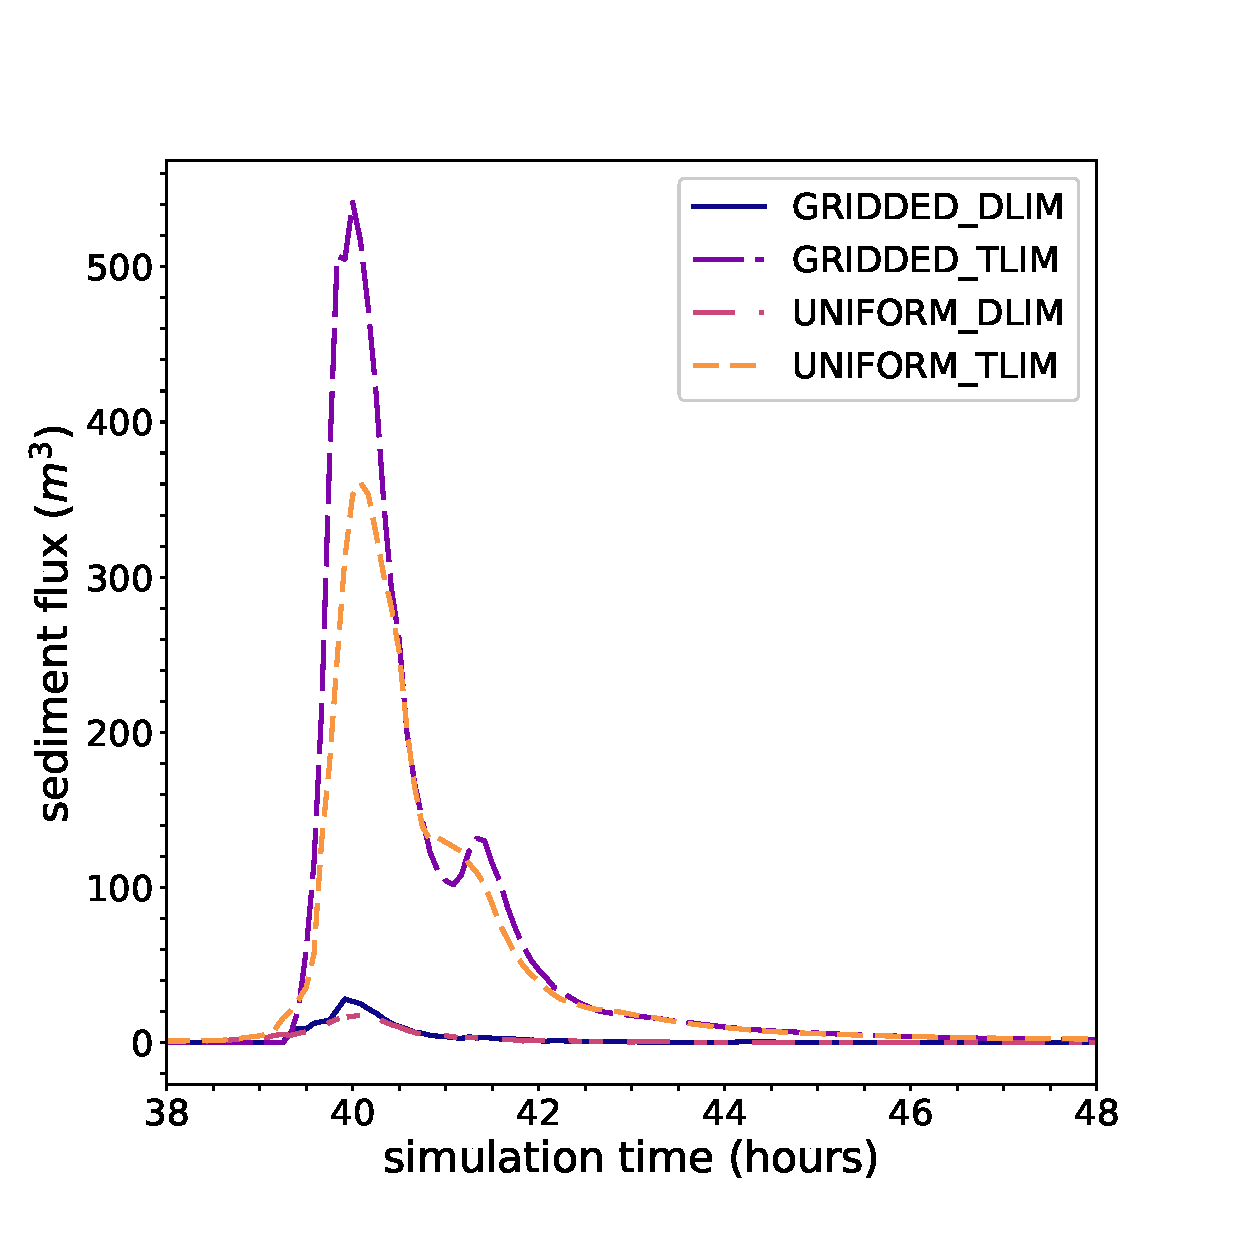
\includegraphics[width=14cm]{chp06_figures_scripts/figure_boscastle_sedigraph_ensemble.eps}
\caption{Boscastle sediment flux (total sediment volume output per hour at catchment outlet for each erosion-enabled simulation of the 2004 Boscastle event listed in Table \ref{table_ensemble_experiments}.}
\label{fig_boscastle_sedigraph_ensemble}
\end{figure}

\begin{figure}[t]
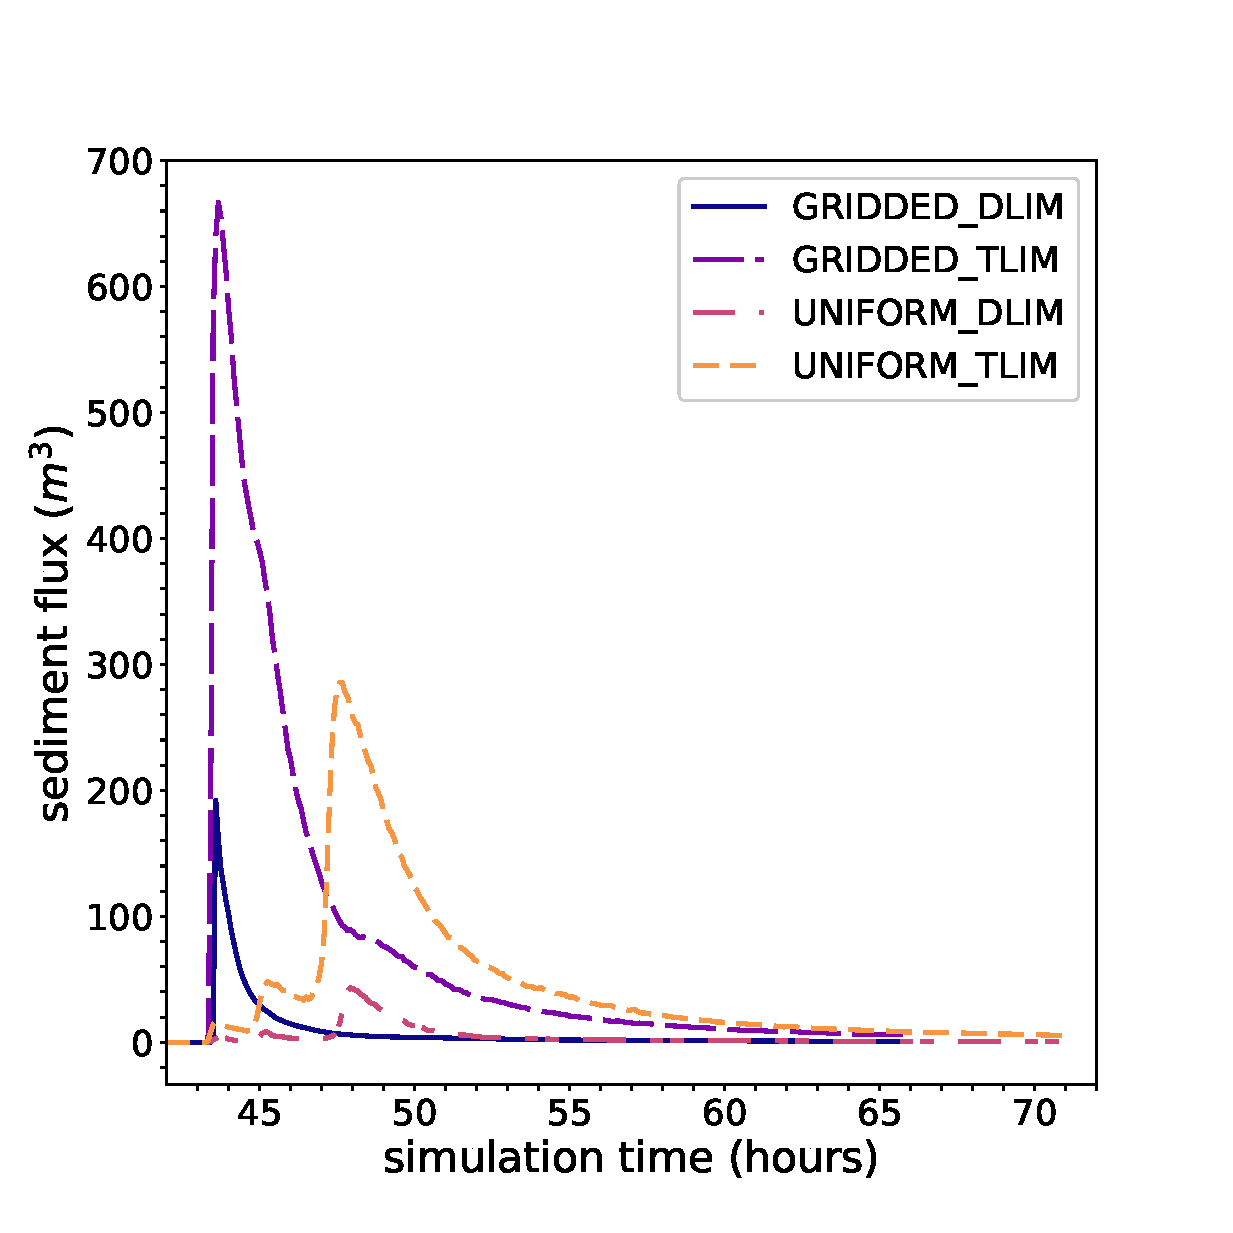
\includegraphics[width=14cm]{chp06_figures_scripts/figure_ryedale_sedigraph_ensemble.eps}
\caption{Ryedale sediment flux (Total sediment volume output per hour at catchment outlet) for each erosion-enabled simulation of the 2005 Ryedale event listed in Table \ref{table_ensemble_experiments}.}
\label{fig_ryedale_sedigraph_ensemble}
\end{figure}

% Describe planform variations in erosion and deposition
\subsection{Spatial variations in sediment and bedrock erosion}
The main spatial variation seen in sediment erosion is seen in river channels, where shear stresses require to initiate erosion and sediment transport are greatest due to the flow of water. The amount of erosion in each simulation was highly sensitive to parameterisation choice of the sediment erosion and transport law, with the choice of rainfall input data (gridded vs uniform) being only a secondary controlling factor on erosion amounts, all other factors being equal. This behaviour was seen on all simulations, in Figure \ref{fig_boscastle_2dplan_erosion_ensemble} and \ref{fig_ryedale_2dplan_erosion_ensemble}. 

To highlight the variation in erosion along the river channel, longitudinal profiles showing the average change in elevation after the storm are shown in Figures \ref{fig_boscastle_swath_tlim} and \ref{fig_ryedale_swath_tlim}. The longitudinal profile shows the variation in erosion along the main channel within each catchment, averaged along a 10 m wide swath centred on the midpoint of the channel. The swath profiling technique is adapted from \citep{hergarten2014extracting}. To reduce the number of points plotted along the swath profile, erosion is also averaged longitudinally, using bins spaced every 200m in the Ryedale catchment and every 50m in the Valency catchment.

% Swath profiles
% Boscastle TLIM
\begin{figure}[htb]
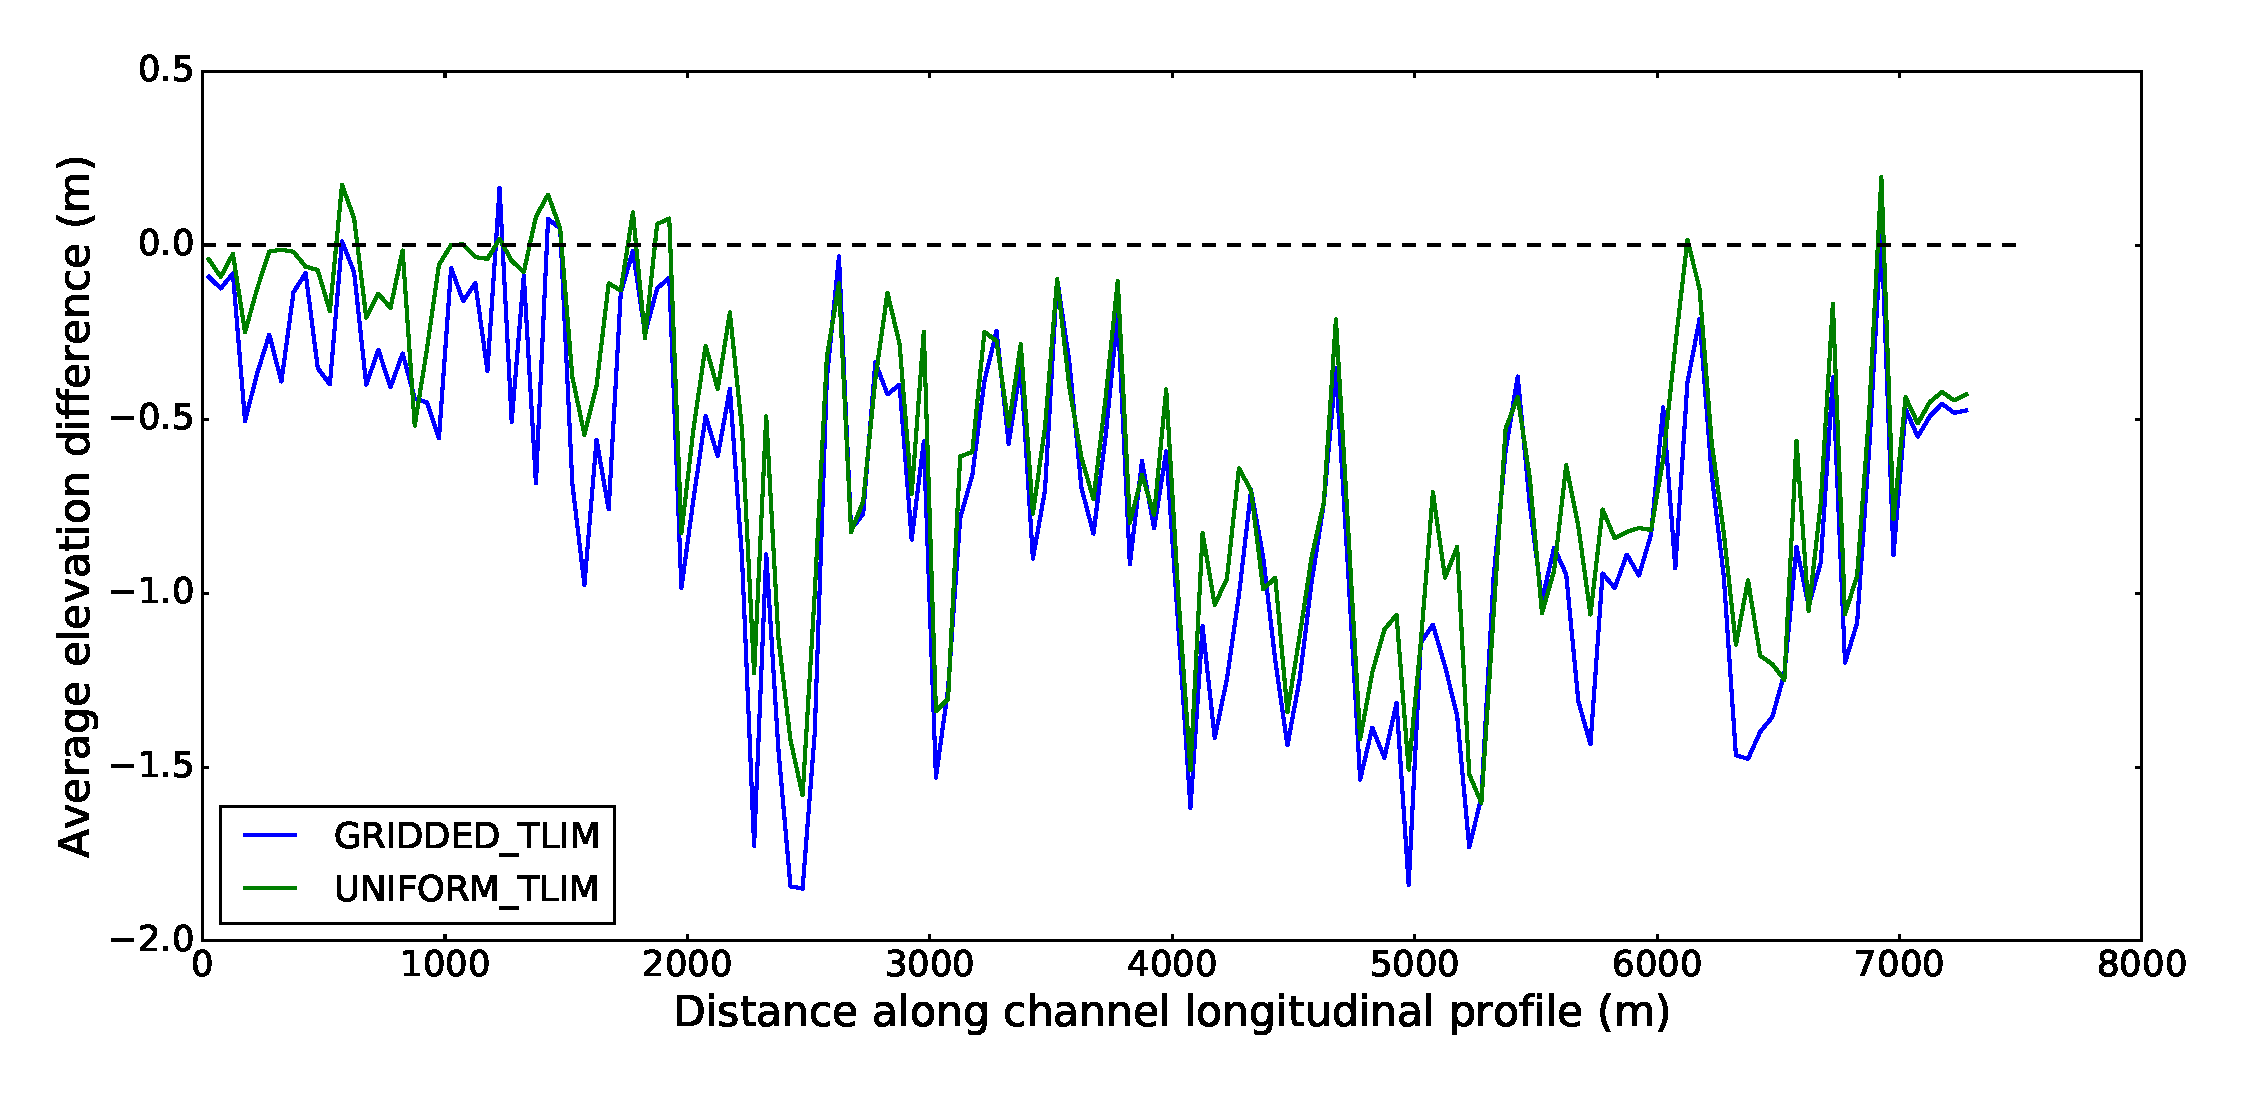
\includegraphics[width=14cm]{chp06_figures_scripts/fig_swath_profile_boscastle_erode_tlim.eps}
\caption{Channel averaged elevation difference along the main river channel in the Valency catchment. Simulation using the transport limited erosion parametrisation. Longitudinal profile is averaged over bins spaced every 50m. Transverse averaging (across the channel) is done over a 10m wide section centred on the channel midpoint. Results from the GRIDDED\_TLIM simulation shown in blue and the UNIFORM\_TLIM simulation shown in green.}
\label{fig_boscastle_swath_tlim}
\end{figure}

% Ryedale TLIM
\begin{figure}[htb]
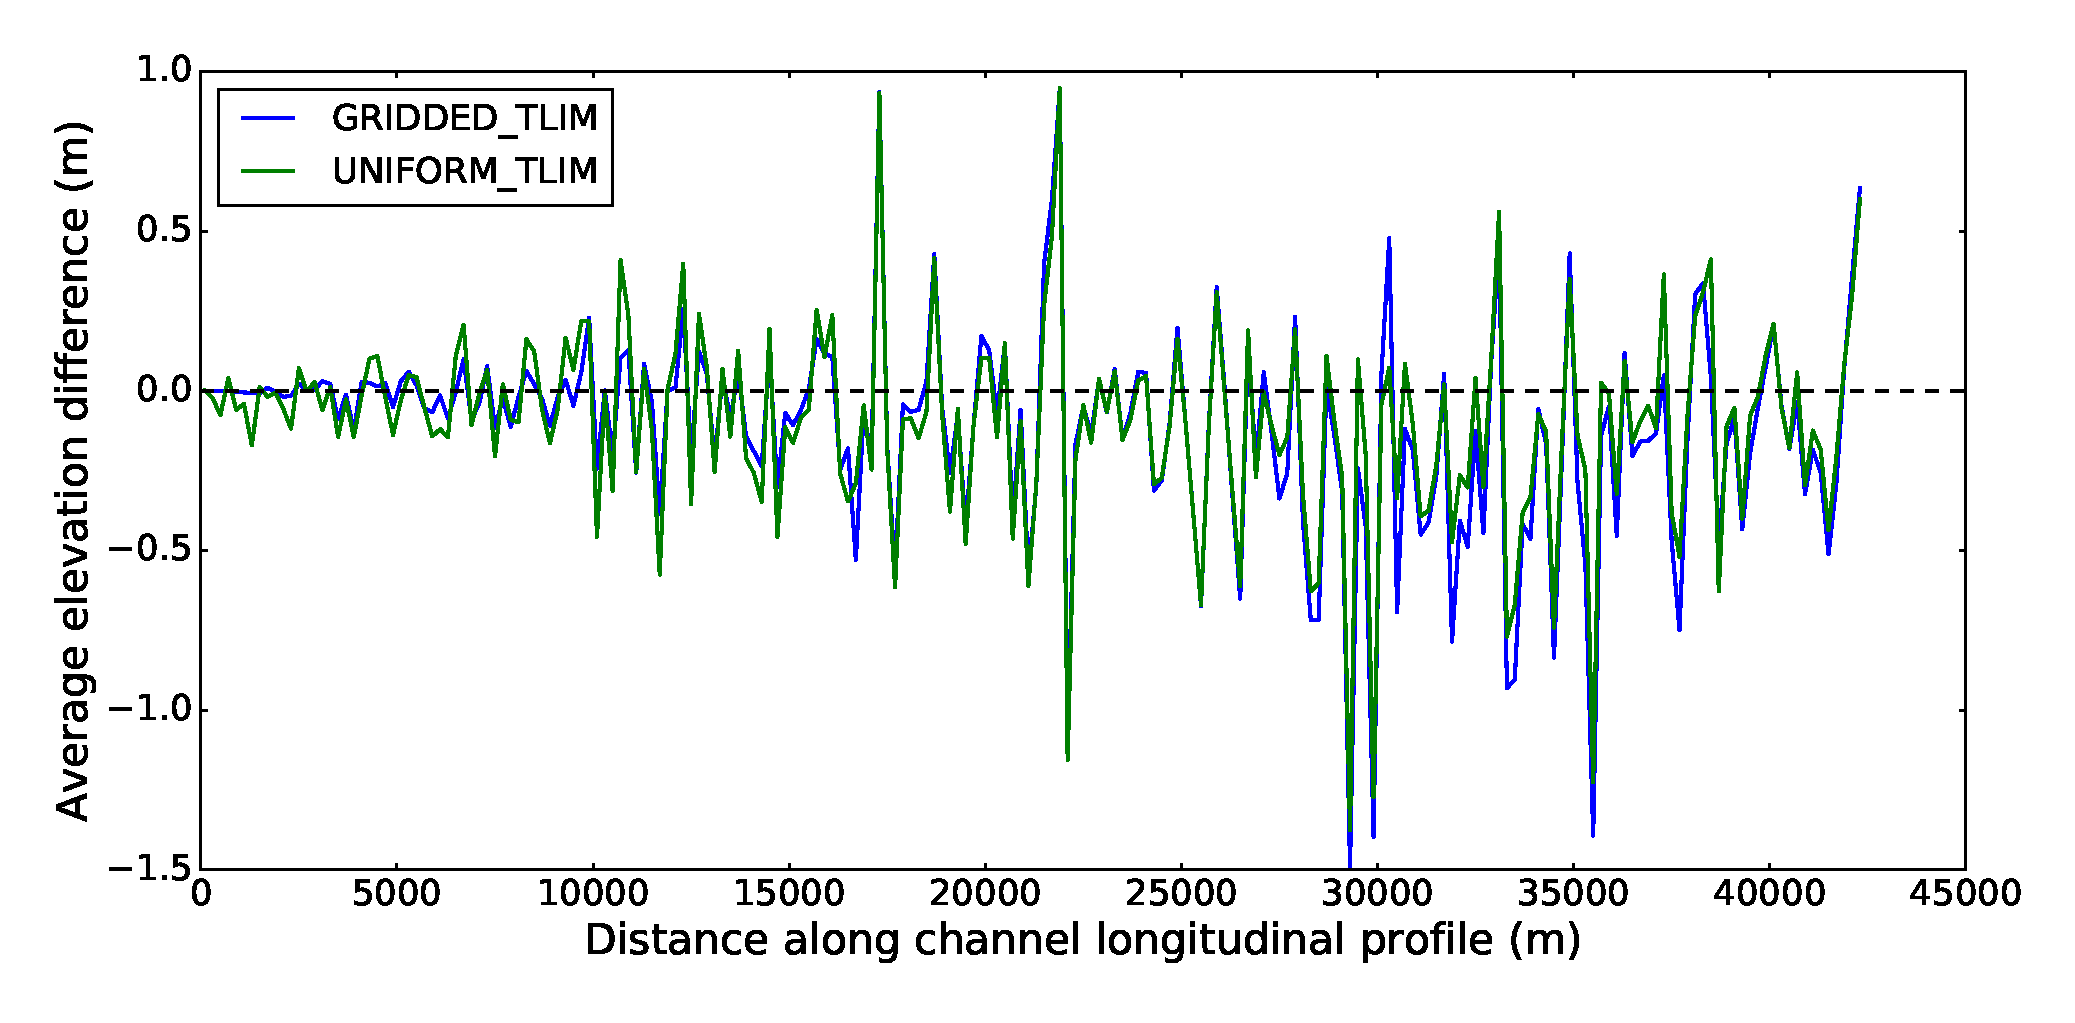
\includegraphics[width=14cm]{chp06_figures_scripts/fig_swath_profile_ryedale_erode_tlim.eps}
\caption{Channel averaged elevation difference along the main river channel in the Valency catchment. Simulation using the transport limited erosion parametrisation. Longitudinal profile is averaged over bins spaced every 50m. Transverse averaging (across the channel) is done over a 10m wide section centred on the channel midpoint. Results from the GRIDDED\_TLIM simulation shown in blue and the UNIFORM\_TLIM simulation shown in green.}
\label{fig_ryedale_swath_tlim}
\end{figure}

Swath profiling of the Valency river channel (Boscastle) shows overall a net incision in the channel area, under transport-limited erosion parameterisation, with only small sections of the channel showing net sediment deposition (elevation increase) on average. Most incision is predicted to occur in the mid to upper reaches of the channel, with relatively little incision in the lowest reach of the catchment. The difference between gridded and uniform rainfall inputs shows a minimal difference along the main profile, though there is a slight tendency for the incision seen in the gridded rainfall input simulation to be higher in most places than the simulation using uniform input, with the difference in incision amounts of the order of tens of centimetres at most.

The swath profiling of the Rye river channel within the Ryedale catchment shows a large variation in incision and deposition rates within the catchment, though there is still an overall tendency for net incision. The magnitude of both incision and deposition is higher in the mid to upper reaches of the Rye river channel, similar to the pattern observed in the Valency river. The differences in average elevation changes are not as clearly distinguishable between the gridded and uniform rainfall input parameterisations, magnitudes of erosional and depositional peaks are slightly higher in the lower reaches of the river channel, but in the mid to upper reaches the differences are more varied. 
 
% OTHER SWATH PROFILES? DLIM, WIDER SWATH HALF WIDTH PERHAPS FOR RYEDALE?????
%
%

% Plan view erosion diff maps
\begin{sidewaysfigure}[t]
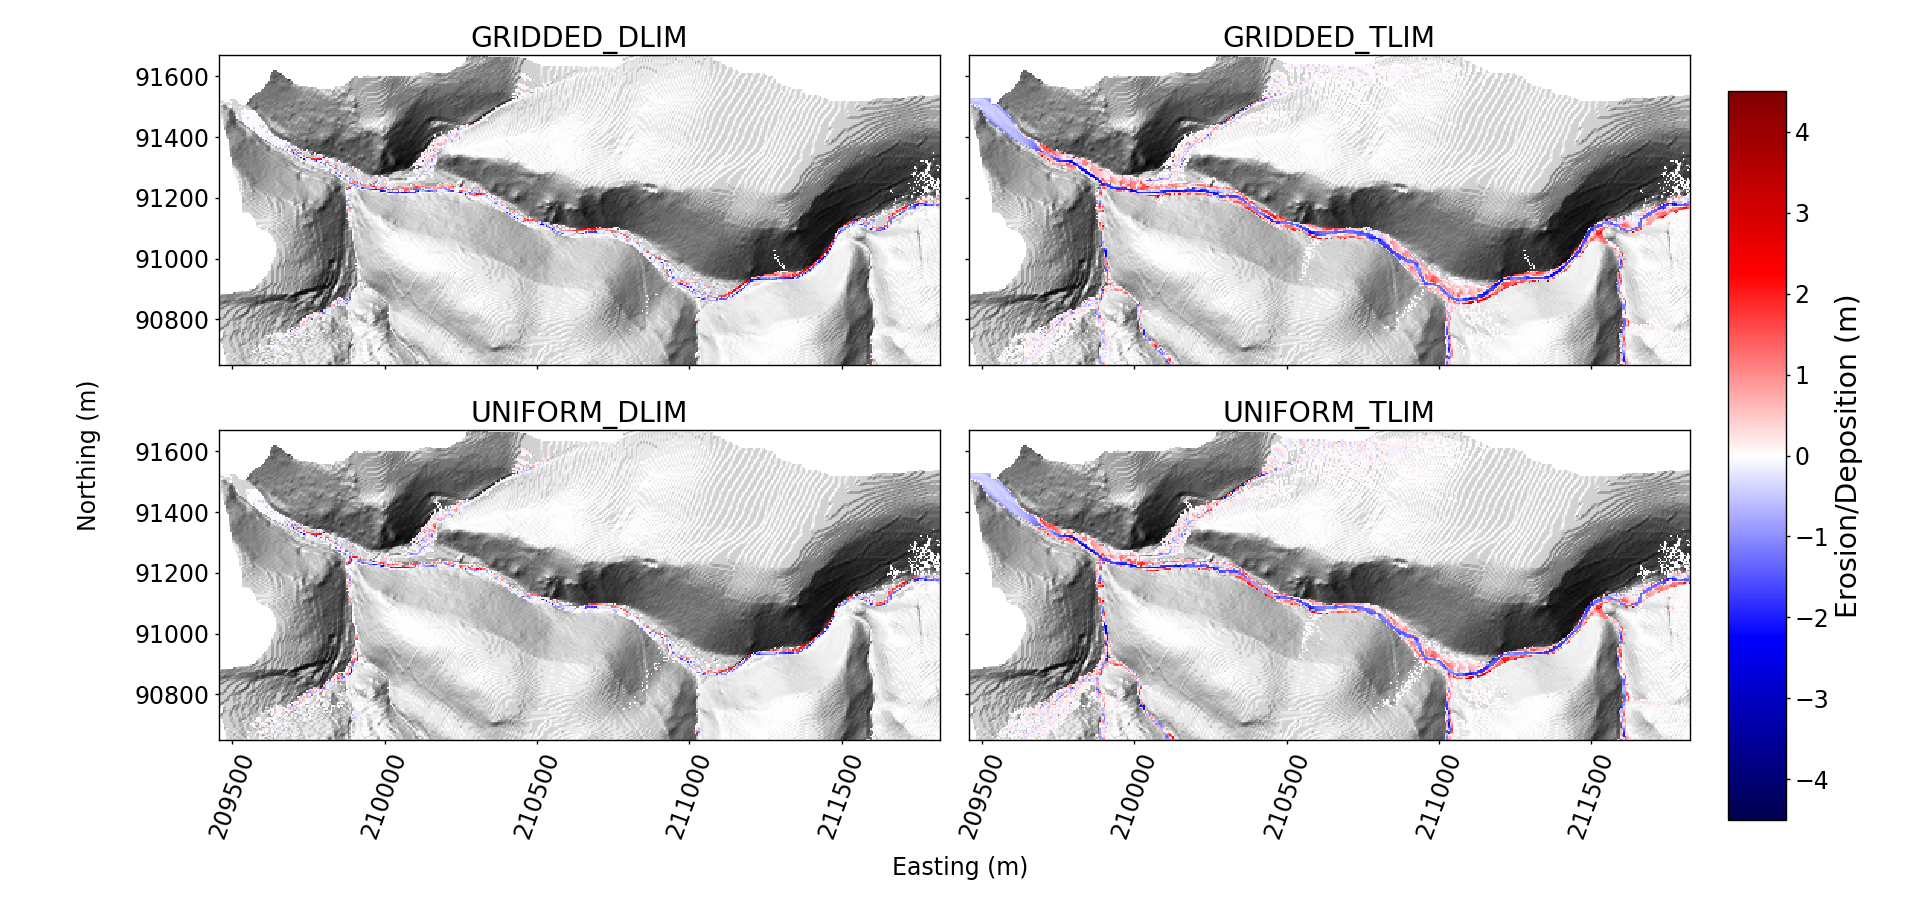
\includegraphics[width=25cm]{chp06_figures_scripts/figure_boscastle_erosion_diff_ensemble.png}
\caption{Boscastle. Erosion.}
\label{fig_boscastle_2dplan_erosion_ensemble}
\end{sidewaysfigure}

\begin{sidewaysfigure}[t]
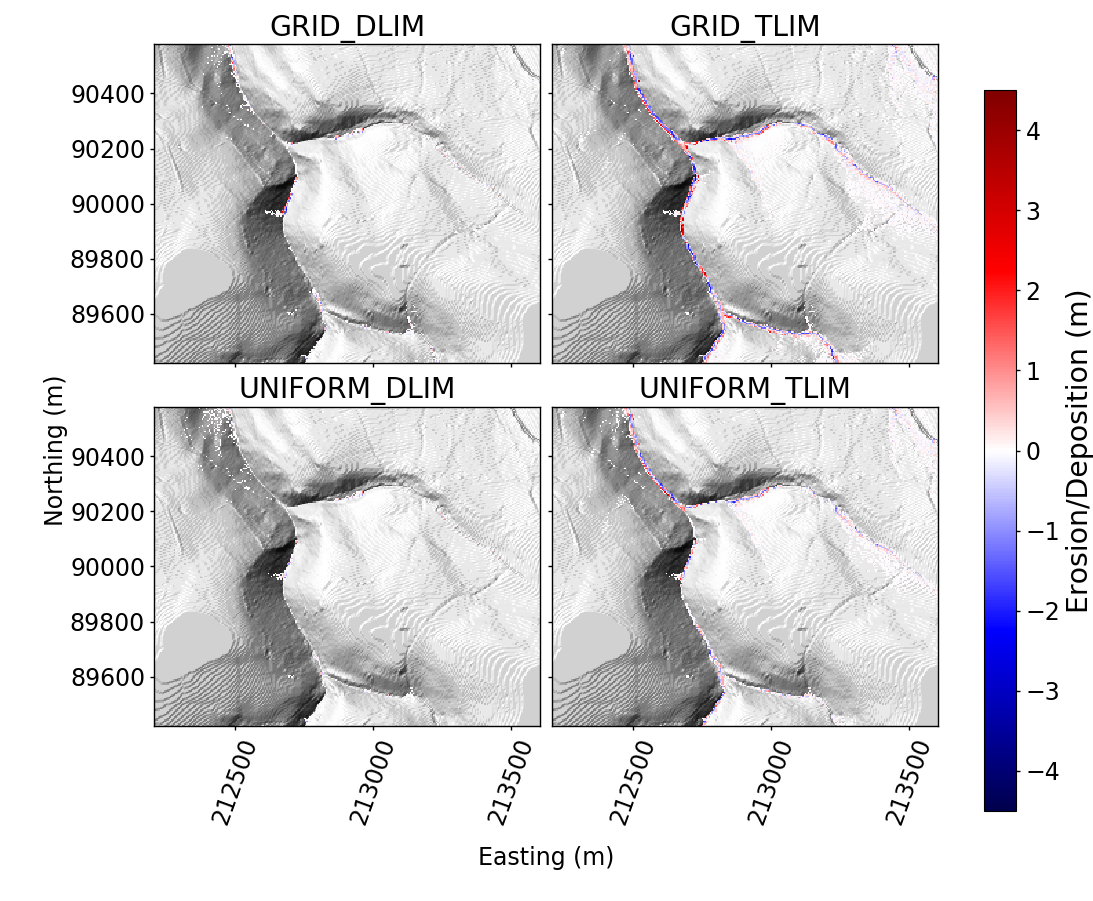
\includegraphics[width=18cm]{chp06_figures_scripts/figure_boscastle_erosion_diff_ensemble_SE.png}
\caption{Boscastle. Erosion. SE trib}
\label{fig_boscastle_2dplan_erosion_ensemble_SE}
\end{sidewaysfigure}

% Plan view erosion diff maps
\begin{sidewaysfigure}[t]
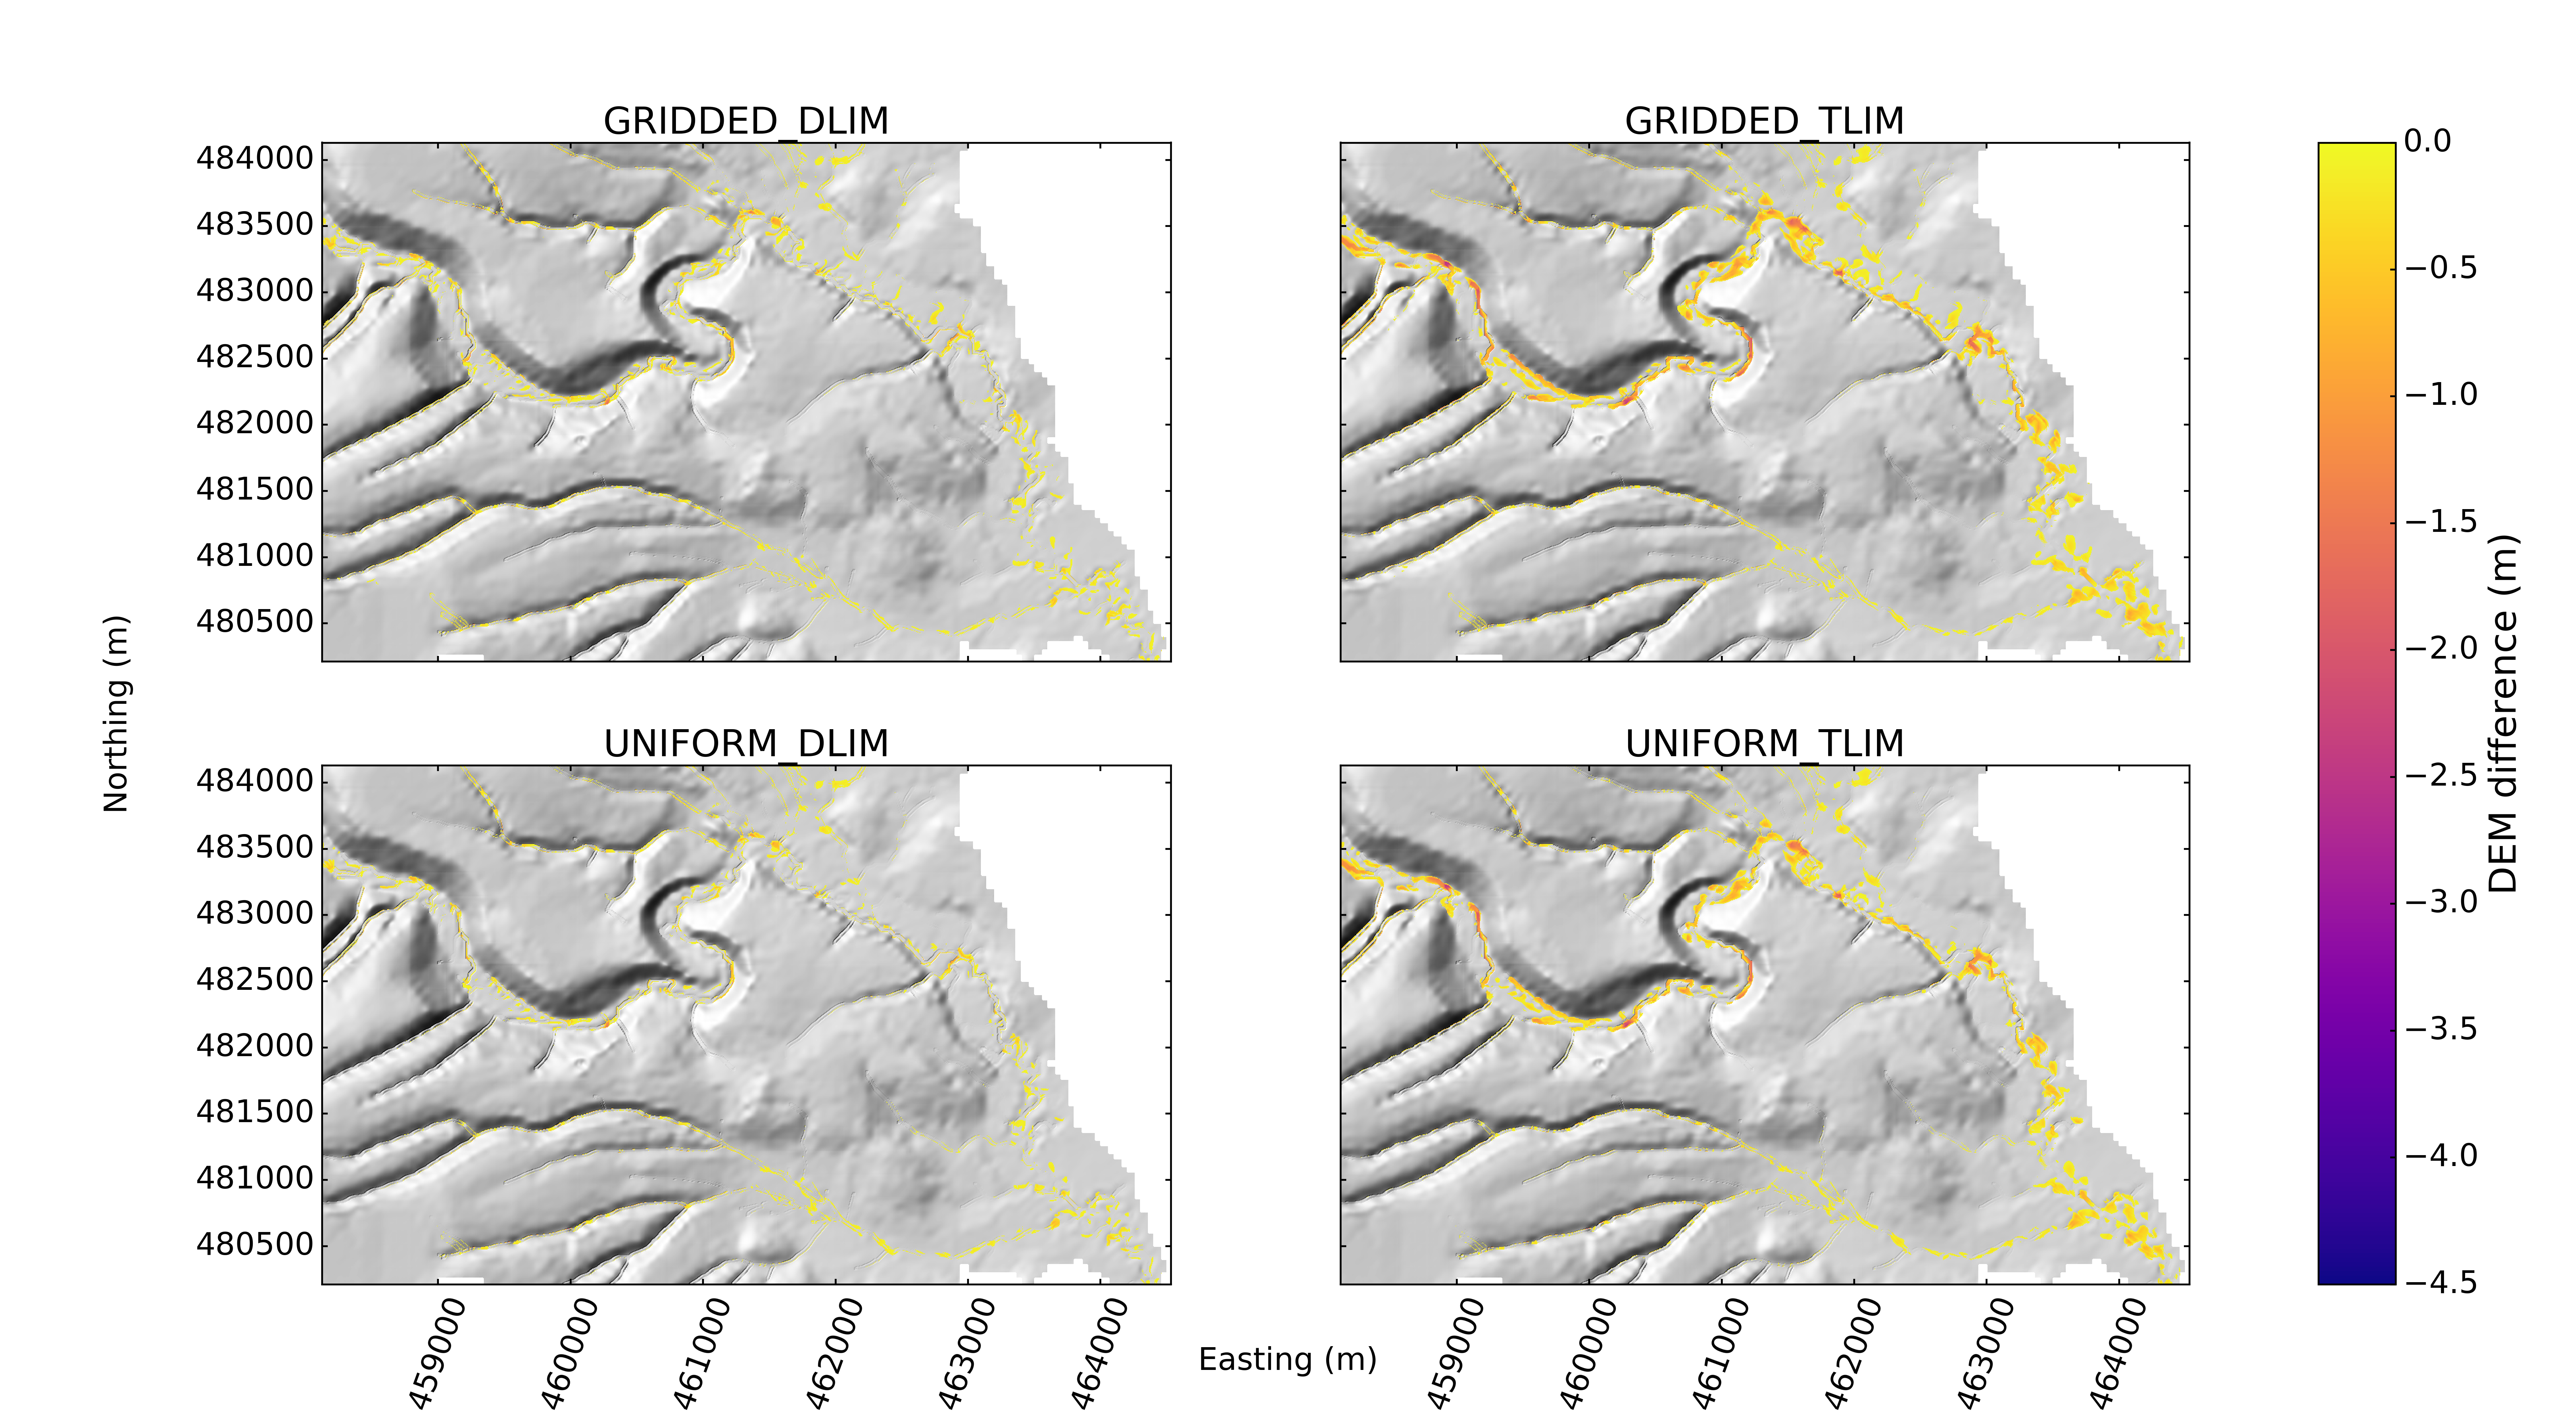
\includegraphics[width=25cm]{chp06_figures_scripts/figure_ryedale_erosion_diff_ensemble.png}
\caption{Ryedale. Erosion.}
\label{fig_ryedale_2dplan_erosion_ensemble}
\end{sidewaysfigure}

% Full extent erosion maps
\begin{sidewaysfigure}[t]
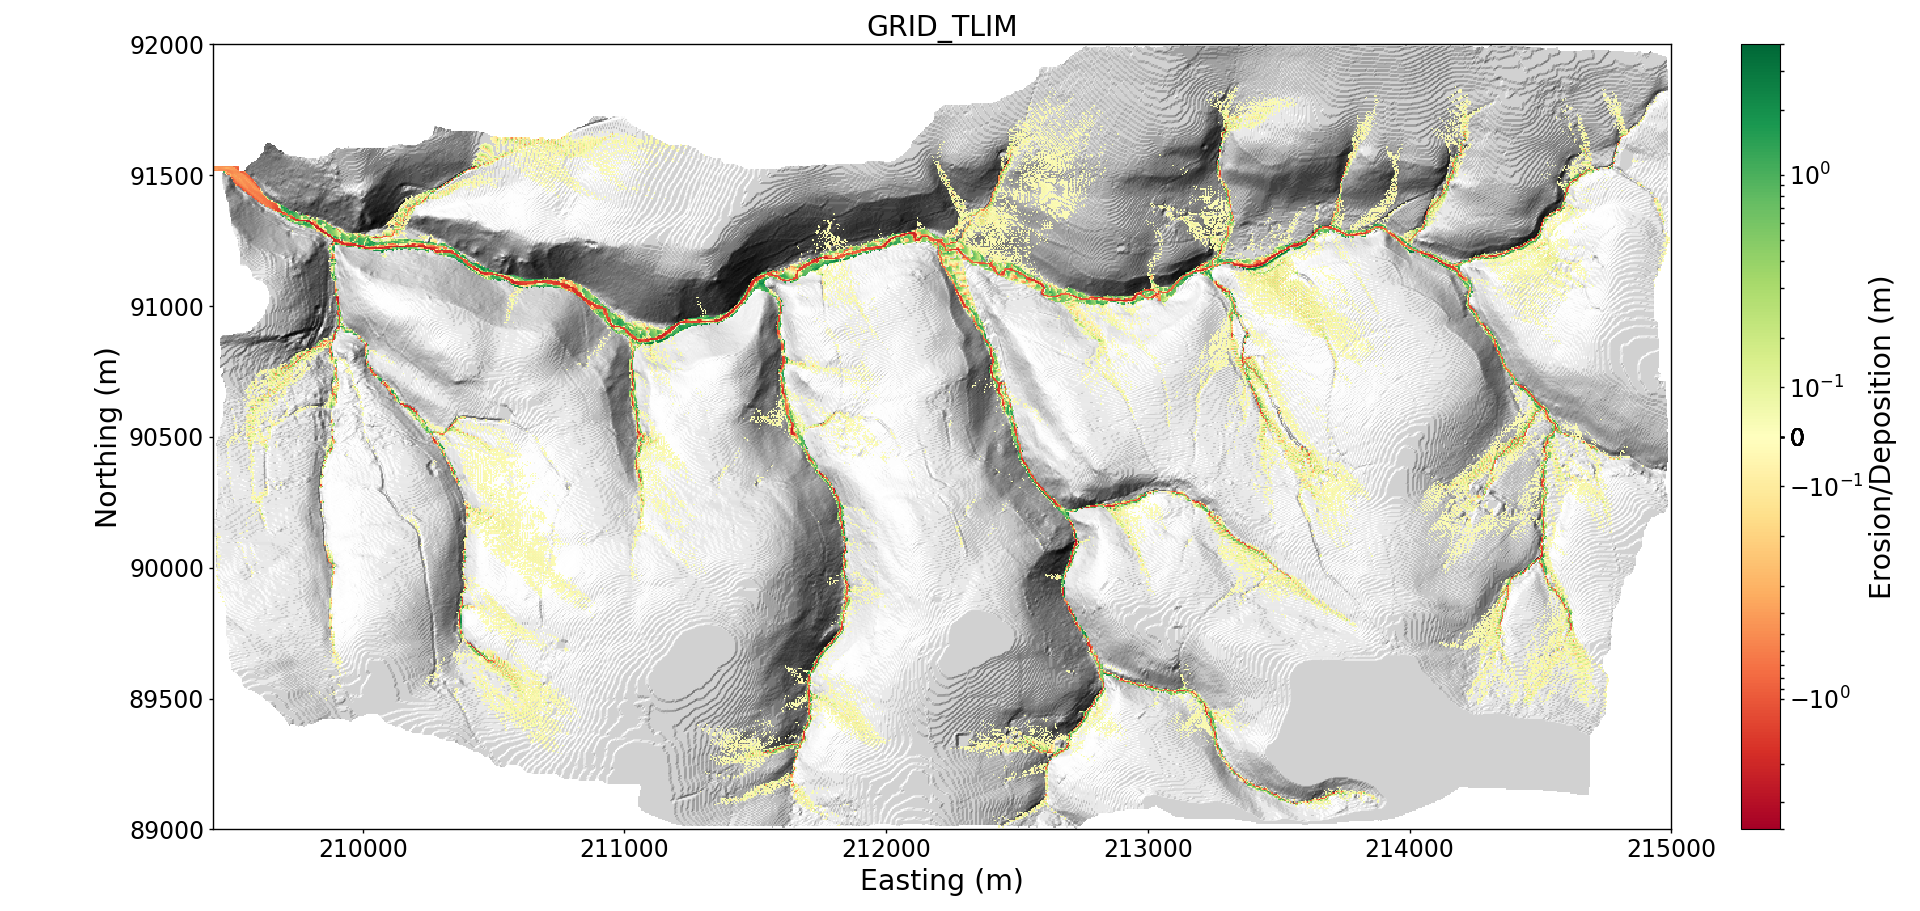
\includegraphics[width=25cm]{chp06_figures_scripts/boscastle_erodediff_grid_tlim.png}
\caption{Boscastle. Map of extent of catchment change in elevation greater than 0.02m. Change in elevation shown after 72 hours of model simulation using gridded rainfall and the transport limited erosion law. (GRID\_TLIM)}
\label{fig_boscastle_erodediff_grid_tlim}
\end{sidewaysfigure}

\begin{sidewaysfigure}[t]
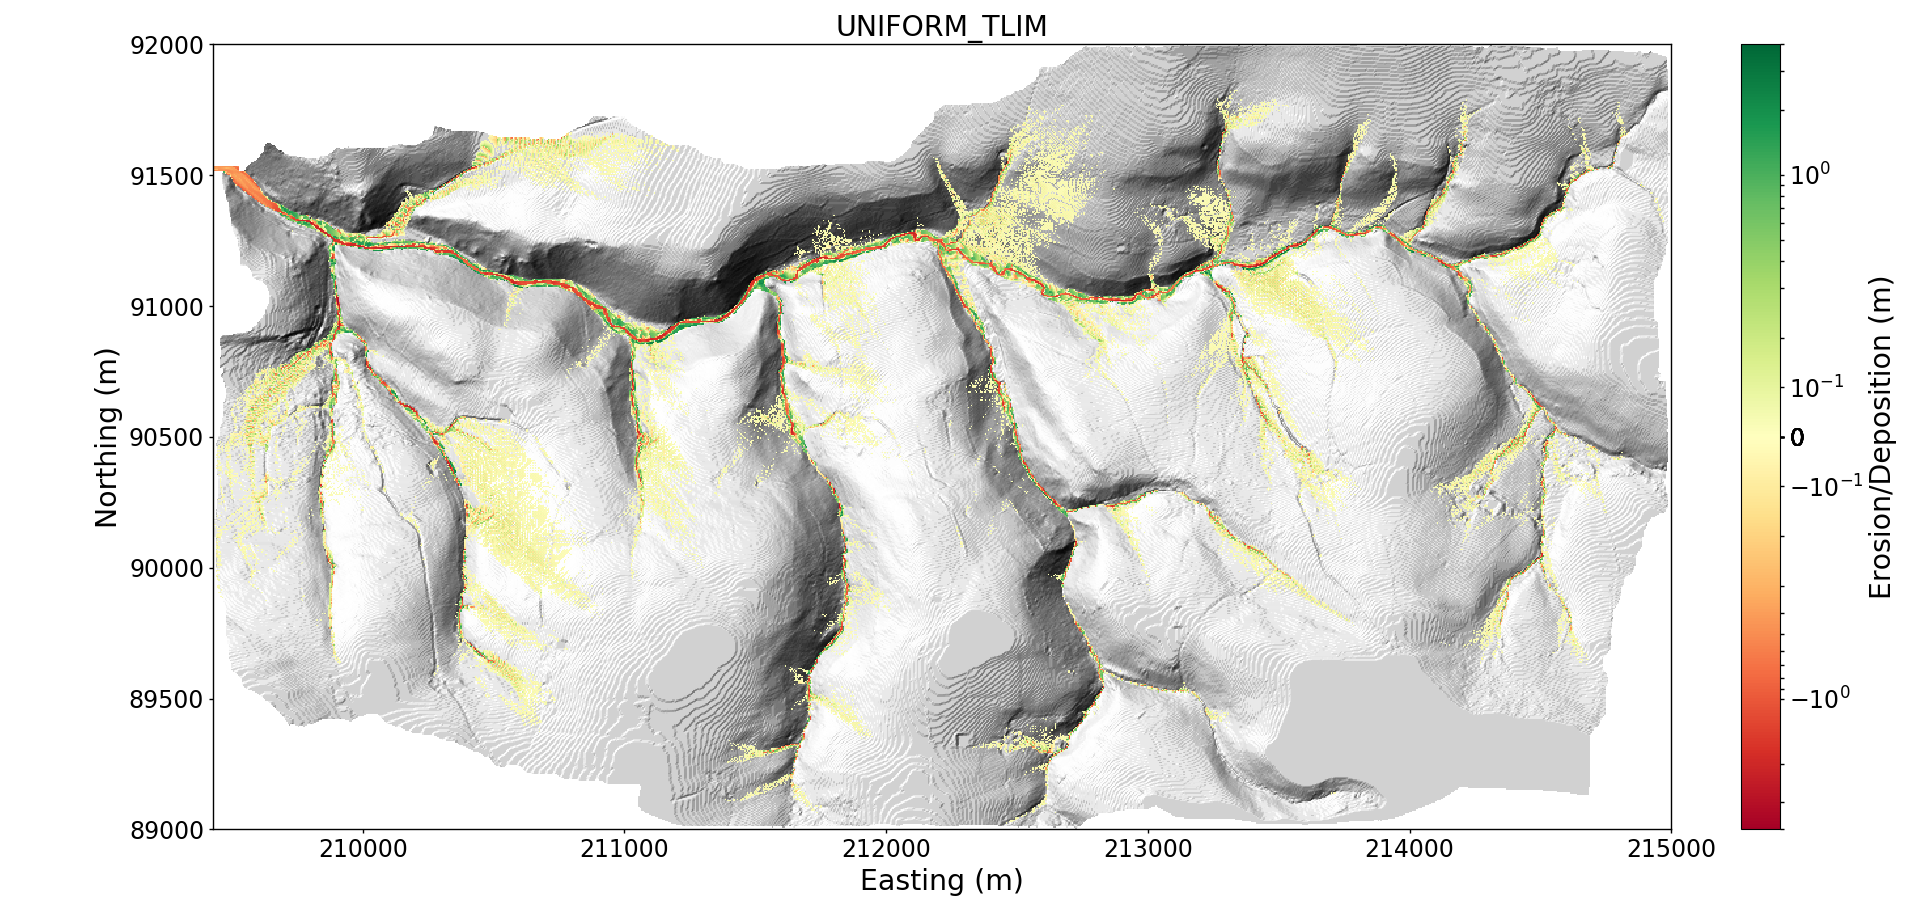
\includegraphics[width=25cm]{chp06_figures_scripts/boscastle_erodediff_uniform_tlim.png}
\caption{Boscastle. Map of extent of catchment change in elevation greater than 0.02m. Change in elevation shown after 72 hours of model simulation using uniform rainfall and the transport limited erosion law. (UNIFORM\_TLIM)}
\label{fig_boscastle_erodediff_uniform_tlim}
\end{sidewaysfigure}

% RYEDALE lower reaches
\begin{figure}[htb]
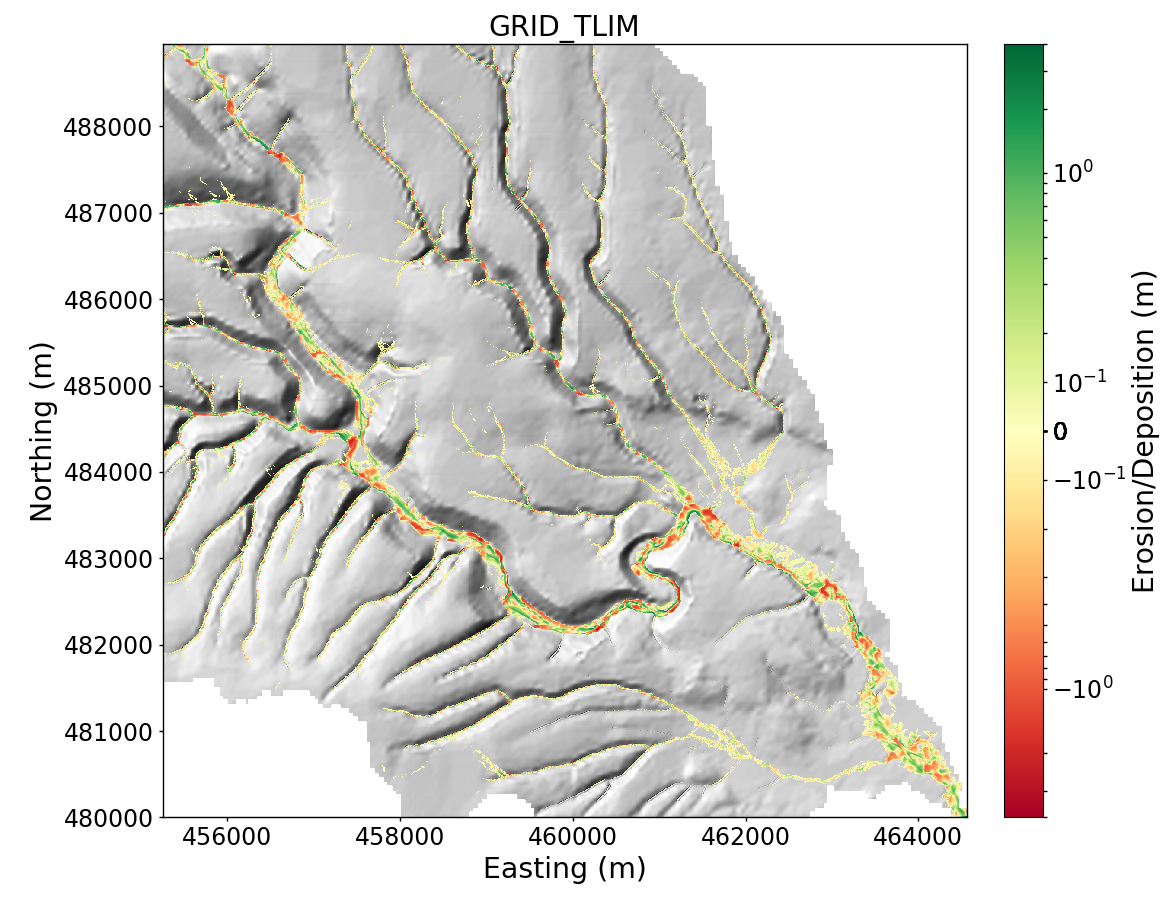
\includegraphics[width=16cm]{chp06_figures_scripts/fig_ryedale_lower_erodediff_grid_tlim.png}
\caption{Ryedale. Map of extent of catchment change in elevation greater than 0.02m. Change in elevation shown after 72 hours of model simulation using gridded rainfall and the transport limited erosion law. (GRIDDED\_TLIM)}
\label{fig_ryedale_erodediff_lower_grid_tlim}
\end{figure}

\begin{figure}[htb]
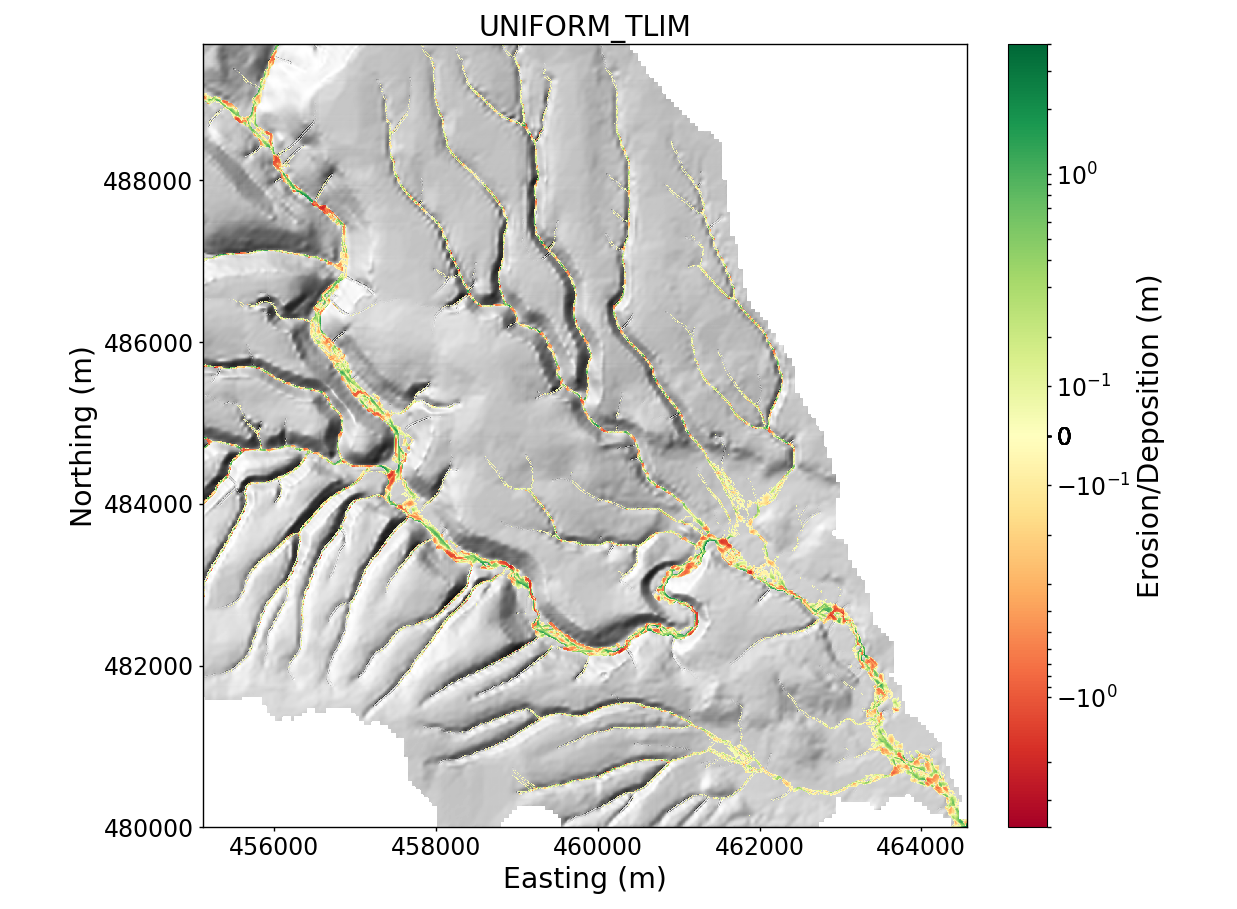
\includegraphics[width=16cm]{chp06_figures_scripts/fig_ryedale_lower_erodediff_uniform_tlim.png}
\caption{Ryedale. Map of extent of catchment change in elevation greater than 0.02m. Change in elevation shown after 72 hours of model simulation using uniform rainfall and the transport limited erosion law. (UNIFORM\_TLIM)}
\label{fig_ryedale_erodediff_lower_uniform_tlim}
\end{figure}

\section{Discussion}

As with hydrology and flood extent (Chapter \ref{chapter_flood_model_sensitivity}), sediment flux exhibits sensitivity to the input rainfall data resolution, but the more dominant sensitivity is to the sediment erosion parameterisation choice in the model. The set of erosion-enabled simulations in these experiments represented two end-members of sediment transport and erosion laws. The \textit{TLIM}-suffixed simulations representing a purely transport limited environment and the \textit{DLIM}-suffixed environment representing a purely detachment limited environment -- with the transport limited law simulations predicting much greater sediment flux and erosion than the detachment limited counterparts. In terms of sediment flux and erosion, the role of rainfall input data spatial resolution played only a secondary role in determining erosion amounts. The size of the catchment was less important in this respect, with even the smaller Boscastle catchment showing a marked sensitivity to the choice of erosion law.

\section{Conclusion}
Over long term landscape evolution, erosional processes in catchments are known to be sensitive to the spatial distribution of rainfall input.  This study has shown that catchment erosional processes are also sensitive to rainfall spatial distribution during the course of a single severe storm, and it is suggested that this is due to the spatial variation in shear stresses required brought on by heterogeneous rainfall inputs to the catchment system.  As sediment transport and erosional process are highly threshold dependent, this leads to erosional patterns that differ according to the pattern of rainfall input. In other words, in the simulation of landscape evolution processes at the catchment scale, the choice of whether to use a uniform value representing the rainfall input, or to use a spatially heterogeneous gridded rainfall data, can have a marked impact on the predicted sediment yields from the catchment. 
In terms of sediment yields, however, these experiments have shown that it is the choice of erosional parameterisation in the model, and not necessarily the resolution of rainfall input data, that has a first-order control on the total sediment yields from a catchment and the magnitude of river channel incision during a simulated event.

Stuff amount rarity of events. Catastrophism.

\subsection{Implications for longer-term landscape evolution}
The experiments presented in this chapter have focused on the hydrogeomorphic response to single severe storm events, events which produced floods with return periods of 1 in 330 years (Ryedale) and 1 in 1300 years (Boscastle). The amounts of river channel incision predicted as a result of these storms is comparable to that predicted by studies of landscape evolution on scales of 1000 years, for example a study of a similar upland river basin by \citep{coulthard2016sensitivity} predicted channel incision amounts of 0.5--5m over 1000 years. The experiments presented here, using the same sediment transport law, predicts comparable incision amounts of channel incision during a single storm. If the flood return periods are assumed to be broadly correct, these simulations suggest that the majority of sediment erosion occurs during rare but high magnitude flood events, rather than through gradual processes or more frequent but lower magnitude events.




%\chapter{Sensitivity of landscape evolution to the details of precipitation patterns using NWP model data}

%\chapter{A spatially-limited storm generation model for long-term landscape evolution modelling}
%\chaptermark{Storm morphology controls on topography}
%
%\section{Intro}
%In landscapes where fluvial processes are the dominant mechanism of sediment erosion and transport, several models of fluvial incision have been proposed that parameterise hydro-meteorological conditions -- the transfer of water from the lower atmosphere to the land surface. Such models include the representation of rainfall input as discrete storm events, e.g. the Poisson pulse model of rainfall input (Tucker and Bras, 2000), models that incorporate the role of limited storm duration relative to runoff-time across the catchment (Solyom and Tucker, 2004), and the nature of orographic precipitation gradients the rainfall-runoff-erosion process (e.g. Anders and Roe, 2006; Han and Gasparini 2015). 
%
%
%\section{Hypothesis (mathematical model)}
%
%\textbf{In short}: Rate of fluvial incision is dependent storm size, depth, and position of storm cell relative to the catchment. This applies to large catchments or small storm cells, where the ratio of storm coverage to total catchment size is less than one. 
%
%\subsection{Catchment hydrology with limited storm cell sizes}
%For large catchments, or for small storm cells, the area of rainfall input, here termed the catchment wetted area, will be less than the total catchment drainage area. (See figure 1). This is denoted by the ratio: \(A_w/A\), where \(A_w\) is the wetted area. 
%
%%\begin{figure}
%%\label{stormcellbasin}
%%%\includegraphics[width=\textwidth]{drawing.png}
%%\caption{Two scenarios in the limited area storm model, both with storm cell areal coverage less than the total basin area. Storm wetted area \(A_{wa} \approx A_{wb}\). a) Storm cell centred far from catchment outlet point, ratio of wetted flow runoff length to max basin length, \(L_w/L\), is near 1. b) Storm cell centred close to outlet point, \(L_w\) is short relative to basin total length. The implications on peak discharge, and thus erosion rates, are discussed within the text.}
%%\end{figure}
%
%Given a catchment with a smaller contributing storm cell, there can be variability in the positioning of the storm relative to the catchment outlet point. This spatial variation in storm cell positioning will influence the storm hydrograph for each storm event. The total storm hydrograph time, \(T_h\) can be given by:
%
%\begin{equation}
%T_h = T_r + T_t
%\end{equation}
%
%Where \(T_r\) is the storm duration time, and \(T_t\) is the total runoff travel time from the most distant wetted point in the catchment to the outlet. The total runoff travel time is given by:
%
%\begin{equation}
%T_t = L_w/U_f
%\end{equation}
%
%where \( L_w \) is the longest wetted flow routing path in the catchment, \(U_f\) is the flow routing velocity, assumed to be approximately spatially constant. 
%
%\subsection{Deriving an approximation for discharge in storm-size limited catchments} 
%Solyom and Tucker (2004) note that similar derivations for peak discharge approximation are needed for environments where storm size is limited relative to catchment area, so I use their equations as a starting point. 
%
%Starting with the simple case of Hortonian (infiltration excess) overland flow, the discharge at a point in the river channel can be given by:
%
%\begin{equation}
%Q = (R - I)A_w
%\end{equation}
%where R is rainfall rate, I is infiltration rate, and \(A_w\) is the upstream wetted drainage area. The total volume of water in a given storm is stated as:
%
%\begin{equation}
%V = (R - I)A_w T_r
%\end{equation}
%
%where \(T_r\) is the storm duration time. As per Solyom and Tucker (2004) the total flood hydrograph volume can be written as:
%
%\begin{equation}
%V = \int_{0}^{T_h} Q(t) dt
%\end{equation}
%
%The hydrograph can be non-dimensionalised by scaling with peak flow, \(Q_p\), and time can be normalised by the total flood hydrograph duration, \(T_h\) (after Willgose, 1989):
%
%\begin{equation}
%Q'(t') = Q(t)/Q_p
%\end{equation}
%where
%\begin{equation}
%t' = t/T_h
%\end{equation}
%
%Then the non-dimensionalised flood-hydrograph volume can be written as such:
%
%\begin{equation}
%V = Q_p T_h \int_{0}^{1} Q'(t') dt'
%\end{equation}
%
%Assuming constant rainfall, \(R\), and infiltration rates, \(I\), peak discharge can be written as a function of runoff rate, storm duration, storm wetted area, and wetted flow route length:
%
%
%%\begin{equation}
%\begin{align}
%\label{peakdischarge}
%Q_p &= \frac{V}{T_h \int_{0}^{1} Q'(t') dt'} \
%    &= \frac{1}{T_h} \frac{(R-I) A_w T_r}{F_{hs}} \
%    &= \frac{(R-I)A_w}{F_{hs}} \frac{T_r}{T_r + L_w/U_f} 
%\end{align}
%%\end{equation}
%
%where \(F_{hs}\) is a hydrograph `shape-factor' equal to the integral in equation (8). \(F_{hs}\) goes to one for steady state run off conditions (i.e. a flat or rectangular hydrograph)
% 
%According to equation \ref{peakdischarge}, peak discharge will vary according to the catchment wetted area to wetted flow runoff length ratio, \(A_w/L_w\), and the ratio of storm duration, \(T_r\), to the total hydrograph duration. Also note that \(A_w\) and \(L_w\) are not independent of each other, and increasing \(A_w\) can increase \(L_w\). (This is not true in the Solyom and Tucker (2004) application of this equation as rainfall is assumed to spatially uniform over the total catchment area.)
%
%\subsection{Assumptions}
%
%\begin{itemize}
%\item Storm cell is stationary (does not track across the basin for the duration of the storm)
%\item Storm cell is a single cell. (i.e. not multiple cells scattered across the basin)
%\item Flow routing velocity is uniform. (Not entirely true assumption, routing time is slower on hillslopes, but the effect can be ignored if drainage density is relatively uniform (Solyom and Tucker (2004)).
%\item Rainfall rate and infiltration rate constant for duration of storm.
%\item Simple infiltration-excess (Hortonian) hydrological state.
%
%\end{itemize}
%It may be possible to modify the model to account for one or more of these assumptions.
%
%
%\subsection{Fluvial erosion}
%(Deriving a similar expression for fluvial incision in a detachment-limited environment here, incorporating the above non-steady discharge approximations for limited storm-area cases) 

%The rate of incision at any given point in a fluvial, bedrock channel is typically given as a function of excess shear stress, that is to say a certain threshold of shear stress exerted by the fluid flow of a river must be exceeded to detach bedrock material (Howard and Kerby, xxxx):

%\begin{equation}
%\epsilon = K_e(\tau - {\tau}_c)^\gamma
%\end{equation}
%
%where shear stress, \({\tau}_c \) and critical shear stress, \( {\tau}_c \), are given by a function of the local discharge \(q\), channel gradient, \(S\) and a shear stress coefficient, \(K_t\).
%
%Traditional models of fluvial incision typically consider discharge at any given point on the landscape as a function of local channel gradient and upstream constributing drainage area, such as the simple stream power law equation for fluvial incision in bedrock channels;
%
%\begin{equation}
%E = 
%\end{equation}


%\chapter{Co-evolution of rainfall patterns and landscapes}
%
%\textit{It would be nice to look at this if there was time (there probably won't be though!) I had a rough framework sketched out and partially implemented for how this would be done using CHILD and WRF together. Maybe one for the future instead.
%}

\chapter{Conclusions}
\label{chapter_conclusion}
\chaptermark{Conclsuions}

The spatial resolution of rainfall input in a river catchment simulation has a demonstrable effect on both hydrological and sediment fluxes, which is seen in both catchment-wide fluxes (Figures \ref{fig_boscastle_hydrograph_ensemble}, \ref{fig_boscastle_sedigraph_ensemble}, \ref{fig_ryedale_hydrograph_ensemble}, \ref{fig_ryedale_sedigraph_ensemble}). Though the magnitude of the sensitivity varied between experiments, there was a general increase in water fluxes, and hence sediment flux, in simulations with gridded rainfall data used as the rainfall input, compared to simulations that used a single, uniform value for rainfall. Existing studies investigating landscape evolution model sensitivity to rainfall resolution \citep{coulthard2016sensitivity} have noted similar increases in water discharge and sediment yields when using spatially heterogeneous rainfall data. The results from the experiments presented in this chapter are broadly in agreement with the general findings of \citet{coulthard2016sensitivity} although the timescales involved in each study are of different magnitudes. The results presented here suggest that the effect of rainfall resolution sensitivity applies to hydrogeomorphic processes at the single-event time scale, as well as landscape evolution over periods of hundreds and thousands of years.

Increasing the resolution of rainfall input data may not be enough to observe sensitivity in smaller catchments, as rainfall features themselves may not exhibit the necessary heterogeneity in structure to benefit from being resolved at finer scale. Rain cells or bands equal to or greater in size than the catchment over which they rain upon, may well be homogeneous enough in spatial extent and rainfall rate that a `uniform' approximation of their rainfall rate is sufficiently precise enough to represent the rainfall rate at all points in the catchment. As seen in the Boscastle catchment simulations, using a detailed rainfall input data source did not notably alter the outcome of the hydrological predictions (Figures \ref{fig_boscastle_2dplan_flood_ensemble}, \ref{fig_ryedale_2dplan_flood_ensemble}). In the Ryedale catchment simulations, the hydrological predictions were notably different based on the choice of rainfall input data resolution, affecting both the time and magnitude of the resulting flood peak. 
%
Talk about size of convective cell features. What is typical storm cell size and heterogeneity (decay from centre?).


% If using biblatex package

\printbibliography

% If using natbib package
%\bibliographystyle{apalike}
%\bibliography{literature}

% Comment the following THREE lines if you do NOT have an Appendix
\appendix
%\chapter{Linking high-resolution NWP model output with a landscape evolution model}
\label{appendix_wrf_lem}
\section{Introduction}

An introduction to the need for better forecasting of flash fooding events. Societal impacts etc. References to recent events in the UK. Rapid geomorphological change can accompany such events, leading to unexpected hydrological outcomes as most models assume static terrain surface during flood-inundation prediction.

Weather forecast models allow high resolution simulations to forecast spatial details of precipitations. Potential forecasting capability when coupled to hydrodynamic landscape evolution model. Relate to summer convective events which tend to be much more spatially focused (mesoscale) and can hence rainfall inputs can vary significantly across a catchment. NWP offers greater lead times than radar `nowcasting'. 

Can cite Pitt review (2008).

Need to investigate better linking of environmental models. E.g. NWP to Land Surface Flooding and Erosion models.

This chapter presents a framework for driving a landscape evolution model with output from NWP simulations. The framework is based upon further enhancements made to the HAIL-CAESAR model, described initially in Chapter \ref{chapter_HAIL-CAESAR}. The enhancements are described in the following section and then tested by the application of the model framework to test cases from intense rainfall events in the UK, previously investigate in Chapter \ref{chapter_hydrogeomorph}.

The work investigates whether a one-way coupled model can provide better forecasting ability over a model driven with coarser resolution rainfall radar data.

\section{Modelling framework}


\section{Method}

Two WRF simulations.

\begin{itemize}
\item Boscastle (2004)
\item Ryedale (2005)
\item Both events triggered flash floods, and the flooding was exarcebated by the mobilisation of sediment during the flood, leading to blocked river channels/channels with reduced capacity.
\end{itemize}

Model set up:
\begin{itemize}
\item Four domains, with the innermost domain centred on the river catchment of interest with a horizontal grid spacing of 200m. Outer domains have reolutions of 25km, 5km, and 1km.
\item Initialised with ECMWF data. (ERA-20C).
\end{itemize}

\textbf{Figure: WRF domain set up}

\textbf{Table: WRF parameters for each simulation}

\subsection{Modifications to the CAESAR-Lisflood model}
Description of model modifications to enable ingestion of high resolution rainfall data. I.e. describe the new rainfall runoff generation model. How it differs from the standard sem-distributed model (TOPMODEL) found in CAESAR-Lisflood.

A f\textbf{figure} would probably be useful here to aid the description of the model component. 

\subsection{Landscape evolution model set up}

No need to repeat the general model description in Chapter 5, just refer back. List the parameters for each simulation in a table though.

\subsection{Modelling framework}

\textbf{Figure: flowchart showing the set up of the two models and their integration}. Brief description here.

\section{Results}

\subsection{NWP modelling results}

\textbf{Show a figure of the rainfall outputs over the inner domain and overlain over the river catchment(2 figures, one for each case)}

\subsection{Landscape evolution/hydrology modelling results.}

Similar figures as to previous chapter of flood inundation and erosion spatial distribution. 

\section{Discussion} 

Discus differences with the rainfall radar chapter previously. Does 200m NWP simulations produce any noticable differences with the 1km gridded radar inputs and the uniform rainfall inputs. 

%\chapter{Linking high-resolution NWP model output with a landscape evolution model}
\label{appendix_wrf_lem}
\section{Introduction}

An introduction to the need for better forecasting of flash fooding events. Societal impacts etc. References to recent events in the UK. Rapid geomorphological change can accompany such events, leading to unexpected hydrological outcomes as most models assume static terrain surface during flood-inundation prediction.

Weather forecast models allow high resolution simulations to forecast spatial details of precipitations. Potential forecasting capability when coupled to hydrodynamic landscape evolution model. Relate to summer convective events which tend to be much more spatially focused (mesoscale) and can hence rainfall inputs can vary significantly across a catchment. NWP offers greater lead times than radar `nowcasting'. 

Can cite Pitt review (2008).

Need to investigate better linking of environmental models. E.g. NWP to Land Surface Flooding and Erosion models.

This chapter presents a framework for driving a landscape evolution model with output from NWP simulations. The framework is based upon further enhancements made to the HAIL-CAESAR model, described initially in Chapter \ref{chapter_HAIL-CAESAR}. The enhancements are described in the following section and then tested by the application of the model framework to test cases from intense rainfall events in the UK, previously investigate in Chapter \ref{chapter_hydrogeomorph}.

The work investigates whether a one-way coupled model can provide better forecasting ability over a model driven with coarser resolution rainfall radar data.

\section{Modelling framework}


\section{Method}

Two WRF simulations.

\begin{itemize}
\item Boscastle (2004)
\item Ryedale (2005)
\item Both events triggered flash floods, and the flooding was exarcebated by the mobilisation of sediment during the flood, leading to blocked river channels/channels with reduced capacity.
\end{itemize}

Model set up:
\begin{itemize}
\item Four domains, with the innermost domain centred on the river catchment of interest with a horizontal grid spacing of 200m. Outer domains have reolutions of 25km, 5km, and 1km.
\item Initialised with ECMWF data. (ERA-20C).
\end{itemize}

\textbf{Figure: WRF domain set up}

\textbf{Table: WRF parameters for each simulation}

\subsection{Modifications to the CAESAR-Lisflood model}
Description of model modifications to enable ingestion of high resolution rainfall data. I.e. describe the new rainfall runoff generation model. How it differs from the standard sem-distributed model (TOPMODEL) found in CAESAR-Lisflood.

A f\textbf{figure} would probably be useful here to aid the description of the model component. 

\subsection{Landscape evolution model set up}

No need to repeat the general model description in Chapter 5, just refer back. List the parameters for each simulation in a table though.

\subsection{Modelling framework}

\textbf{Figure: flowchart showing the set up of the two models and their integration}. Brief description here.

\section{Results}

\subsection{NWP modelling results}

\textbf{Show a figure of the rainfall outputs over the inner domain and overlain over the river catchment(2 figures, one for each case)}

\subsection{Landscape evolution/hydrology modelling results.}

Similar figures as to previous chapter of flood inundation and erosion spatial distribution. 

\section{Discussion} 

Discus differences with the rainfall radar chapter previously. Does 200m NWP simulations produce any noticable differences with the 1km gridded radar inputs and the uniform rainfall inputs. 

\chapter{Code availability}

\chapter{Key code and algorithms for the cellular automaton LEM}

\chapter{Key components and algorithms for the additions to the CHILD model}

%\chapter{Modifications made to the Weather Research and Forecasting model (WRF)}

%\chapter{A one-way coupling framework for the WRF-CHILD model}

\chapter{Cluster computing simulations: set-up, compilation, and scaling}

\chapter{Paper off-prints may also be attached with a traditional-format thesis}


% If you need more than one appendix, then just use another \chapter command
%\chapter{Yet Another Appendix}

\end{document}
